
\documentclass[12pt,a4paper,twoside]{book}
\usepackage{subfigure}
\usepackage{amsmath}
\usepackage{mathrsfs}
\usepackage{wasysym}
\usepackage{lineno}
\usepackage{authblk}
\usepackage{rotating}
\usepackage{rotfloat}
%\usepackage{color}
\usepackage{multirow}
\usepackage{xspace}
\usepackage{rotating}
\usepackage{hyperref}
\usepackage{enumitem}
\usepackage{cite}
%\usepackage[margin=1.in]{geometry}
\usepackage{geometry}
%\usepackage[sorting=none]{biblatex}
\hypersetup{pdfborder = 0 0 0}
%\usepackage[titletoc]{appendix}
%\usepackage{graphicx}
%\usepackage{caption}
%\usepackage{subcaption}

% \usepackage{feynarts} 
\listfiles
%%%%%%%%%%%%%%%%%%%%%%%%%%%%%%%%%%%%%%%%%%%%%%%%%%%%%%%%%%%%%%%%%%%%%%%%%%%%%%%
% This is where the document really begins
%%%%%%%%%%%%%%%%%%%%%%%%%%%%%%%%%%%%%%%%%%%%%%%%%%%%%%%%%%%%%%%%%%%%%%%%%%%%%%%

% Shorthand for \phantom to use in tables
\newcommand{\pho}{\phantom{0}}
\newcommand{\bslash}{\ensuremath{\backslash}}
\newcommand{\BibTeX}{{\sc Bib\TeX}}

% Org def
\newcommand{\mT}{\ensuremath{m_{\mathrm{T}}}\xspace}
%\def\mT{\ensuremath{M_{\mathrm{T}}}}
\def\rqcd{\ensuremath{r_{\mathrm{QCD}}}\xspace}
\def\kqcd{\ensuremath{k_{\mathrm{QCD}}}}
\def\rwjets{\ensuremath{r_{W\mathrm{+jets}}}}
\def\kwjets{\ensuremath{k_{W\mathrm{+jets}}}}
\def\rztautau{\ensuremath{r_{Z\rightarrow\tau\tau}}}
\def\rother{\ensuremath{r_{\mathrm{other}}}}
\def\kztautau{\ensuremath{k_{Z\rightarrow\tau\tau}}}
\def\kother{\ensuremath{k_{\mathrm{other}}}\xspace}
\def\mVis{\ensuremath{M_{\tau\tau}^{\mathrm{visible}}}\xspace}
\def\nOSmVis{\ensuremath{n_{\mathrm{OS}}(m_{\mathrm{vis}})}}
\def\nOSqcd{\ensuremath{n_{\mathrm{OS}}^{\mathrm{QCD}}}}
\def\nOSwjets{\ensuremath{n_{\mathrm{OS}}^{W\mathrm{+jets}}}}
\def\nOSztautau{\ensuremath{n_{\mathrm{OS}}^{Z\rightarrow\tau\tau}}}
\def\nOSother{\ensuremath{n_{\mathrm{OS}}^{\mathrm{other}}}}
\def\nSSall{\ensuremath{n_{\mathrm{SS}}^{\mathrm{all}}}}
\def\nSSqcd{\ensuremath{n_{\mathrm{SS}}^{\mathrm{QCD}}}}
\def\nSSwjets{\ensuremath{n_{\mathrm{SS}}^{W\mathrm{+jets}}}}
\def\nSSztautau{\ensuremath{n_{\mathrm{SS}^{Z\rightarrow\tau\tau}}}}
\def\nSSother{\ensuremath{n_{\mathrm{SS}}^{\mathrm{other}}}}
\def\nSSallmVis{\ensuremath{n_{\mathrm{SS}}^{\mathrm{all}}(m_{\mathrm{vis}})}}
\def\nSSqcdmVis{\ensuremath{n_{\mathrm{SS}}^{\mathrm{QCD}}(m_{\mathrm{vis}})}}
\def\nSSwjetsmVis{\ensuremath{n_{\mathrm{SS}}^{W\mathrm{+jets}}(m_{\mathrm{vis}})}}
\def\nOSztautaumVis{\ensuremath{n_{\mathrm{OS}}^{Z\rightarrow\tau\tau}(m_{\mathrm{vis}})}}
\def\nSSztautaumVis{\ensuremath{n_{\mathrm{SS}}^{Z\rightarrow\tau\tau}(m_{\mathrm{vis}})}}
\def\nOSothermVis{\ensuremath{n_{\mathrm{OS}}^{\mathrm{other}}(m_{\mathrm{vis}})}}
\def\nSSothermVis{\ensuremath{n_{\mathrm{SS}}^{\mathrm{other}}(m_{\mathrm{vis}})}}
\def\ttbar{\ensuremath{t\bar{t}}\xspace}
\def\PT{\ensuremath{p_{T}}\xspace}
\def\pt{\ensuremath{p_{T}}\xspace}
\def\GeV{\ensuremath{\text{GeV}}\xspace}
\def\Zee{\ensuremath{Z\rightarrow ee}\xspace}
\def\Zmumu{\ensuremath{Z\rightarrow \mu\mu}\xspace}
\def\Ztautau{\ensuremath{Z/\gamma^*\rightarrow \tau\tau}\xspace}
\def\Ztt{\ensuremath{Z\rightarrow \tau\tau}\xspace}
\def\Wlnu{\ensuremath{W\rightarrow \ell \nu}\xspace}
\def\Zll{\ensuremath{Z\rightarrow \ell \ell}\xspace}
\def\nqcd{\ensuremath{n^{QCD}}\xspace}
\def\rqcd{\ensuremath{R_{QCD}}\xspace}
\def\ToTauTauLepHad{\ensuremath{\rightarrow\tau\tau\to \ell\tau_{had}}\xspace}
\def\ToTauTauLepLep{\ensuremath{\rightarrow\tau\tau\to \tau_{\ell}\tau_{\ell}}\xspace}
\def\MET{\ensuremath{E_{T}^{miss}}\xspace}
\def\met{\ensuremath{E_{T}^{miss}}\xspace}
\def\Ht{\ensuremath{H_{T}}\xspace}
\def\etcone{\ensuremath{E_{T}(\mathrm{cone})} }
\def\ptcone{\ensuremath{p_{T}(\mathrm{cone})} }
\def\SumLtMET{\ensuremath{p_{T\mu} + p_{Te}+\met} }
\def\mmc{\ensuremath{m_{\tau\tau}^{MMC}} }
\def\MMC{\ensuremath{MMC_{mass}} }
\def\mA{\ensuremath{M_{A}}}
\def\mh{\ensuremath{M_{h}}}
\def\mH{\ensuremath{M_{H}}}
\def\mHp{\ensuremath{M_{H^\pm}}}
\def\ifb{\ensuremath{fb^{-1}} }

\linespread{1.27}
\begin{document}
\tableofcontents

%\clearpage
%%%%%%%%%%%%%%%%%%%%%%%%%%%%%%%%%%%%%%%%%%%%%%%%%%%%%%%%%%%%%%%%%%%%%%%%%%%%%%%
%%									     %%		
%%			TRAMA DELLO PSYCHO-TRILLER			     %%
%%									     %%	
%%%%%%%%%%%%%%%%%%%%%%%%%%%%%%%%%%%%%%%%%%%%%%%%%%%%%%%%%%%%%%%%%%%%%%%%%%%%%%%
%%%%%%%%%%%%%%%%%%%%%%%%%%%%%%%%%%%%%%%%%%%%%%%%%%%%%%%%%%%%%%%%%%%%%%%%%%%%%%%
%%  Elementi importanti:                                                     
%%	Statistica ; Descrizione degli oggetti come ele, mu ecc..	     
%%	Data MC sample ; Embedding  ; MMC ;  Corrections	
%%
%%  Struttura Analisi part:
%%	*) motivazioni ; 											| Sezione riguardante quello che ti proponi di fare
%%	*) Strategia: Quale e' la nostra Hypotesis 0, vogliamo fare un test di ipotesi (prima parte Stat).. 	|
%%	   punti chiave che differenziano MSSM higgs da SM e la strategia per sfruttarne i vantaggi (b-tag veto)|
%%	   Selezioni spiegando bene le motivazioni di ciascuna	(full preselections in appendice)		|
%%         MMC													|
%%
%%	*) Background Modeling: Impatto con la realta' delle cose (data driven bkg estimation del quale non ci sarebbe bisogno se tutto fosse perfetto)   | come lo
%%	   quindi si presenta un Problema e ne si da' la soluzione (bkg estimation)									  | Fai
%%	   Data MC sample, Embedding 															  |
%%	*) determinazione sys, che pero' possono essere splittate in due ---> una in tesi l'altra in appendix (che non ce ne frega una sega dei dettagli) |
%%	
%%	*) Risultati:  parte aggiuntiva su stat. e limiti.
%%
%%	
%%
%%  Struttura resto:	
%%	*) Theory   
%%	*) Atlas detector + descrizione degli oggetti + performance + corrections
%%	*) Trackjets
%%
%%  Try to not suicide...	
%%
%%
%%
%%
%%
%%
%%
%%
%%
%%
%%

\chapter{Introduction}

 
The Standard Model of particle physics is a theory that describes at quantum level the interacion 
between matter and radiation. It is a very predictive and succesfull theoretical framework
which has been largely confirmed by experimets.  The recent discovery of a new boson of mass
$\sim 126$~GeV by the ATLAS and CMS experiments~\cite{AHiggsO,CHiggsO} at Large Hadron Collider 
in agreement with the SM prediction is another success of this theory.
The most recent measurements \cite{ASpin0,ACouplings,CFermions,CWidth} of its
properties shows this new boson to be, within experimental uncertainties, fully
compatible with the SM Higgs boson. However, it remains an open question
whether this new particle is the only missing piece of the electroweak symmetry breaking
sector or whether it is one of several Higgs bosons predicted in  theories 
that go beyond the SM. Among all of them, Supersymmetry  is a theoretically favoured scenario
as the most predictive framework beyond the Standard Model. Chapter~\ref{chap:theory} of this thesis 
is devoed to introduce the Minimal Supersymmetric extension of the Standard Model, focusing 
in particular on its Higgs sector, with a description of the expected neutral MSSM Higgs bosons
phenomenology.

The search presented in this thesis is based on 20.3 $\text{fb}^{-1}$ of proton-proton collision data at 
a centre-of-mass energy of $\sqrt{s} = 8$~TeV recordered by the ATLAS experimet at the LHC during 2012.
An overview of the ATLAS experiment and of the Large Hadron Collider complex is given in Chapter~\ref{chap:detector}. 
The data recordered by the ATLAS experiment need to undergo several steps of offline reconstruction 
before being ready for analysis, the physics object reconstruction and quality criteria used are described in 
Chapter~\ref{chap:obj}.

The main topic of this thesis is the search for the neutral MSSM Higgs bosons decaying into pairs of tau leptons,
each subsequently decaying into an electron or muon and two neutrinos.
This final state correspond to 6\% of the total branching fraction of a di-tau leptons system decays, even limited by the BR
this final state has a competitive sensitivity with the other channels at low mass.
The search is performed for the two most significant production modes, gluon fusion and in association with
b-quarks. The search is performed in two complementary event catergory, either with or without reconstructed b-jet
and are optimized separately. Chapter~\ref{chap:anal}.

In general the Higgs bosons produced in association with b-quark is carachterized by the presence of relatively low-transverse momentum
jets (originating from b-quarks), the reconstruction and calibration of calorimeter jets suffers strongly for such a low transverse
momentum, which is one of the main reason for sensitivity loss in the category that requires a tagged jet.
An alternative approach would be to 

Chapter~\ref{chap:trackjet}.



%Theory
\newgeometry{left=4.5cm, right=4.5cm,bottom=4cm, top=4cm}

\chapter{The Higgs Bosons and the MSSM} \label{chap:theory}

 \vspace{2cm}

This chapter is devoted to introduce the theoretical background to the experimental search presented in this thesis.
A brief overview of the Standard Model of particle physics is given in Section~\ref{sec:SM} based on Reference~\cite{Altarelli}. 
Among all the extension of the Standard Model, the Minimal Supersymmetric 
extension of the Standard Model (MSSM) is a theoretically favoured scenario as one of the most predictive
framework beyond the Standard Model. The MSSM is introduced in Section~\ref{sec:MSSM} with focus on its Higgs sector, based on 
References~\cite{SusyPrimer,Djuadi}.
Finally, a review of the MSSM Higgs bosons phenomenological aspects which are relevant to the presented search is given 
in Section~\ref{sec:pheno}, based on Reference~\cite{LHCxsec}.
%In section... introduction is given based on~\cite{Altarelli}, 
%This chapter is devoted to introduce the the Minimal Supersymmetric 
%extension of the Standard Model (MSSM) whit focus on  its Higgs sector.
%In section... introduction is given based on~\cite{Altarelli}, 

\restoregeometry

\clearpage

\section{The Standard Model of Particle Physics} \label{sec:SM}
\subsection{Introduction}
A detailed description of the Standard Model of particle physics may be found in Reference~\cite{Peskin}, only a brief overview is
given in what follows.

The Standard Model (SM) of particle physics is a theory aimed to describe and quantitatively predict
the phenomenology of fundamental interactions. At ``microscopic''  level the spectrum of all interactions between matter and 
radiation can be understood in terms of three classes of fundamental forces: the strong, the electromagnetic
and the weak forces. These interactions are described by a local relativistic quantum field theory, where to each particle
is associated a field with suitable transformation properties under the Lorentz group.
The theory is based on the principle of gauge invariance, which means invariance under  a symmetry  transformations    
that operates on basic internal degrees of freedom and depends on the space-time coordinate.
The gravitational force is negligible in atomic and nuclear physics, in fact,
quantum effects of gravity are expected at energies corresponding to the Planck mass $E \sim M_{planck} c^2 \sim 10^{19}$~GeV.

The SM is a gauge field theory based on the symmetry group $SU(3)_c \otimes SU(2)_L \otimes U(1)_Y$. The group has $8+3+1=12$
generators with a non trivial commutator algebra. The electromagnetic and weak interactions~\cite{EW1,EW2,EW3}  are described  by the 
$SU(2)_L \otimes U(1)_Y$ symmetry group, while the $ SU(3)_c$ is the colour group of the theory of strong interactions (QCD)~\cite{qcd1}.
To each generator of the symmetry group is associated a vector boson which act as mediator of the corresponding interactions.
Eight gluons are associated to the $ SU(3)_c$ colour generators, while  four gauge bosons $W^{\pm}$,
$Z^0$ and $\gamma$ are associated to the generators of $SU(2)_L \otimes U(1)_Y$. 
Only the gluons and the photon are massless since the symmetry induced by the other three generators is
spontaneously broken. In the SM the spontaneous symmetry breaking is realised by the Higgs mechanism~\cite{ENGLERT,HIGGS,HIGGS2,HIGGS3,kibble}.
The Higgs boson acts as mediator of a new class of interactions that, at tree level, are coupled in proportion to the particle masses.
An Higgs boson with properties that resemble the one of the SM 
has recently been discovered at the LHC with $m_H \sim 126$~GeV \cite{AHiggsO,CHiggsO}. %and represents one of the major milestone of particle physics.

The fermionic matter fields of the SM are quarks and leptons. 
Quarks  are subject to all SM interactions, each type of quark is a colour triplet and carries 
electroweak charges, in particular electric charges $+2/3$ for up-type quarks and $-1/3$
for down-type quarks.  Leptons are colourless
but have electroweak charges, in particular electric charge $-1$ for charged leptons $e$, $\mu$ and $\tau$ (opposite sign charge 
is intended for respective anti-particle)  and charge 0 for neutrinos $\nu_e$, $\nu_{\mu}$ and $\nu_{\tau}$.
Qarks and leptons are grouped in three  ``generations'' with equal quantum numbers but different masses.


\subsection{Precision Test and Limitation of the SM}

The Standard Model has been successfully tested in a vast number of experiments over a wide range of energies during the last few decades.
Precision tests of the electroweak theory performed at LEP, SLC and the Tevatron~\cite{smtest}, 
has confirmed that the couplings of quark and leptons to the weak gauge bosons $W^{\pm}$  and $Z$ are indeed
precisely those prescribed by the gauge symmetry. The accuracy of a few per-mille for these
tests implies that, not only the tree level, but also the structure of quantum corrections has
been verified. Several other experimental results~\cite{pdg}
including rare decays of hadrons provides low-energies test of the Standard Model. 
The recent discovery of a Higgs boson  is also another success of the SM, its mass, spin and couplings 
are in agreement with expected values from a global fit of electroweak constraints~\cite{gfitter}.

Among all the parameters of the Standard Model only few of them presents tension with experimental data, 
the most significant discrepancies are slightly above three standard deviations and are given by: the anomalous magnetic moment 
of the muon~\cite{gminus2}, $a_{\mu}$  and the forward-backward asymmetry of top quarks~\cite{FBasymmetry}, $A_{FB}^{\ttbar}$.   


In spite of this success, the Standard Model is conceptually unsatisfactory for quite few deficiencies and is
widely believed to be an effective theory valid only at the present accessible energies. Beside the fact that 
it does not  include  gravitational force, it does not explain the pattern of fermion masses and in its simplest 
version does not include neutrino masses, it has at least other three conceptual problems which indicates the need 
for physics Beyond the Standard Model (BSM):
%\begin{itemize}
%\item
\paragraph{Hierarchy Problem} Calculating the radiative correction to the Higgs boson mass, quadratic divergences occur of the order  
	of the cut-off scale $\Lambda$, where  $\Lambda$ defines  the energy
	beyond which the theory ceases to be valid and new physics should appear~\cite{Lambda}. If the cut-off is chosen 
	to be $\sim M_{Planck}$, then a fine tuning  with an unnaturally high precision , $\mathcal{O}(10^{-30})$, should occur to cancel these divergences 
	leaving the Higgs boson with a mass of the order of the electroweak breaking scale, $M_{EW}$.
	A question that has no satisfactory answer in the SM is how these cancellations can occur and why $\Lambda >> M_{EW}$, these problems are
	called the fine-tuning and hierarchy problem~\cite{Hierarchy1,Hierarchy2,Hierarchy3}.
	%Supersymmetry was first introduced to answer this question, indeed, the new symmetry prevents the Higgs boson mass to acquire very large 
	%radiative corrections, the quadratic divergent loop of the SM particles are exactly cancelled by the loop contribution 
	%of the corresponding partners, solving in this way the hierarchy problem~\cite{Djuadi5}.

%\item
\paragraph{Dark Matter}   The SM does not have a candidate which can explain the large contribution 
	of non-barionic, non-luminous matter to the density of the Universe~\cite{darkmatter1,darkmatter2,darkmatter3}. To be a Dark Matter candidate a particle should be
	stable, massive and should interact only via very weak interactions. 
	%Supersymmetry models,  provided with R-parity conservation,
	%provides a natural candidate for Dark Matter, which would be then the lightest SUSY particle which cannot further decay.

%\item 
\paragraph{Unification Problem}	Another unsatisfactory aspect of the SM is that does not provide the unification of the electroweak and strong interactions,
	their couplings do not meet at high energies. Considering the successful unification of electromagnetic and weak
	interaction, the existence of Grand Unified Theory (GUT) has been 
	suggested~\cite{GUT1,GUT2}, which predicts the unification of all the three gauge coupling strength at the GUT energy scale,
	$\Lambda_{GUT} \simeq 10^{16}$~GeV and describes the three forces within a single gauge group with just one coupling constant.
	%The particle spectrum in SUSY, instead, contributes to the renormalisation group evolution of the three gauge couplings constants and 
	%favours them to meet at energies around $10^{16}$ GeV~\cite{djuadi4}. 

%\end{itemize}
\vspace{0.5cm}
Among all the extension of the SM, Supersymmetry is a theoretically favoured scenario as the most predictive framework beyond the Standard Model.
As discussed in Section~\ref{sec:MSSM}, it gives a natural answer to the hierarchy problem, provides a suitable candidate for Dark Matter
and predicts unification of the three gauge couplings at GUT energy scale.


% the conceptual situation with the
%standard model is unsatisfactory for quite a few deficiencies:
%– the smallness of the electroweak scale v ∼ 246GeV << MPl (the ‘hierarchy problem’);
%– the large number of free parameters (gauge couplings,
%vacuum expectation value, MH, fermion masses,
%CKM matrix elements), which are not predicted but have
%to be taken from experiments;
%– the pattern that occurs in the arrangement of the
%fermion masses;
%– the missing way to connect to gravity.
%
%-Dark matter
%
%-neutrino masses

 
\section{The Minimal Supersymmetric Standard Model}\label{sec:MSSM}
\subsection{Introduction to the MSSM}
Supersymmetry (SUSY)~\cite{Susy1,Susy2,Susy3} was first introduced as a natural way to solve the hierarchy problem.
In Supersymmetry a new symmetry that relates bosons to fermions is introduced.
The SUSY generators $\mathcal{Q}$ transforms fermion into bosons and vice versa:
\begin{equation}
\mathcal{Q}|\text{Fermion}\rangle = |\text{Boson}\rangle, ~ ~ ~ \mathcal{Q}|\text{Boson}\rangle = |\text{Fermion}\rangle
\end{equation}
In a supersymmetric extension of the SM  each of the known fundamental particles 
is in either a chiral or gauge \emph{supermultiplet} and must have a superpartner with spin differing by 1/2 unit.
SUSY naturally solve the hierarchy problem since the quadratic divergent loop contribution to the Higgs mass of the SM 
particles are cancelled by the loop contribution of the corresponding superpartners. 
The name of the superpartner of the quarks and leptons are made by adding an ``s'' to the SM name, standing for scalar.
Accordingly, the gauge bosons related to the generator of the group $SU(3)_c \otimes SU(2)_L \otimes U(1)_Y$ should also have a spin 1/2 partner,
whose name will be made by adding a ``ino'' at the end of the SM name. The symbol of superpartners is defined by adding a ($\tilde{ ~ }$) to the SM symbol.
The SUSY particles share the same couplings with their SM partner, since the left-handed and right-handed components of fermions 
transform differently under gauge transformations also their superpartner present this feature.

The  Minimal Supersymmetric extension of the Standard Model  (MSSM)~\cite{MSSM1,MSSM2,MSSM3,MSSM4,MSSM5,MSSM6}, 
is defined by requiring the minimal gauge group (i.e., the SM one)
and the minimal particle content: three generation of fermions (without right-handed neutrinos), gauge bosons and two Higgs doublet, 
each with its own superpartner. Tables~\ref{tab:chiralsup} and~\ref{tab:gaugesup} summarise chiral and gauge supermultiplets in the MSSM.
Among the gauge eigenstates summarised in these tables, the superpartner of the Higgs bosons, the \emph{higgsinos} mix with the \emph{wino}
and \emph{bino} to give the ``ino'' mass eigenstates: two charginos $\chi_{1,2}^\pm$ and four neutralinos $\chi_{1,2,3,4}^0$.
\begin{table}
\begin{center}
\renewcommand{\arraystretch}{1.5}
\begin{tabular}{c|ccc}
\hline%\noalign{\smallskip}
Names 			&Supermultiplets	&	Spin 1/2  		& Spin 0 \\%[0.1cm]
\hline%\noalign{\smallskip}		
quark, squarks		& $Q$ 			&	$(u_L ~ d_L)$		& $( \tilde{u}_L ~ \tilde{d}_L)$ \\%[0.1cm]
($\times$ 3 families)	& $\bar{u}$		& 	$u_R^{\dagger}$ 	& $\tilde{u}_R^*$ \\%[0.1cm]
			& $\bar{d}$		& 	$d_R^{\dagger}$ 	& $\tilde{d}_R^*$ \\%[0.1cm]
\hline%\noalign{\smallskip}
leptons, sleptons	& $L$			&   	$(\nu ~ e_L)$ 		&  $( \tilde{\nu} ~ \tilde{e}_L)$\\%[0.1cm]
($\times$ 3 families)	& $\bar{e}$		&	$e_R^{\dagger}$         & $\tilde{e}_R^*$ \\%[0.1cm]
\hline%\noalign{\smallskip}
higgsinos, Higgs	& $H_1$			&	$( \tilde{H}_1^0 ~ \tilde{H}_1^-)$  &	$( H_1^0 ~ H_1^-)$ \\%[0.1cm]	 
			& $H_1$			&	$( \tilde{H}_2^+ ~ \tilde{H}_2^0)$  &	$( H_2^+ ~ H_2^0)$ \\%[0.1cm]	 
\hline
\end{tabular}
\caption{This table is based on Reference~\cite{SusyPrimer} and summarise the chiral supermultiplets in the Minimal Supersymmetric Standard Model. The spin-0 fields are complex scalars
	and the spin-1/2 are left-handed two-component Weyl fermions.}
\label{tab:chiralsup}
\end{center}
\end{table}

\begin{table}
\begin{center}
\renewcommand{\arraystretch}{1.5}
\begin{tabular}{c|ccc}
Names			&Supermultiplets& Spin 1 		&	Spin 1/2 \\
\hline
gluons, gluinos		&$G_a$ (a =1,...,8)	& $g$			& $\tilde{g}$	\\
W bosons, winos		& $W_a$ (a=1,...,3)	& $W^{\pm}$ $W^0$	& $\tilde{W}^{\pm}$ $\tilde{W}^0$ \\
B boson, bino		&$B$			& $B^0$			& $\tilde{B}^0$ \\
\hline
\end{tabular}
\caption{This table is based on Reference~\cite{SusyPrimer} and summarise the gauge supermultiplets in the Minimal Supersymmetric Standard Model.}
\label{tab:gaugesup}
\end{center}
\end{table}

\subsubsection{$R$-parity conservation}
The MSSM requires a discrete and multiplicative symmetry called $R$-parity~\cite{Susy3}, this symmetry assures barion and lepton number 
conservation and it is defined as follows:
\begin{equation}
R_p = (-1)^{2s+3B=L}
\end{equation}
where $L$ and $B$ are lepton and barion numbers and $s$ stands for the spin quantum number. The R-parity quantum number has value $+1$ for ordinary
SM particles and $-1$ for their superpartners. This symmetry was first introduced as a simple way to overcome the problem of instability of the proton.
Lepton and barion number violation leads, in many cases, 
to unstable proton with life-time shorter than the experimental lower limit. The conservation of $R$-parity has also other important 
phenomenological consequences: SUSY particles are always produced in pairs and decays always in an odd number of SUSY particles.
Furthermore, the lightest SUSY particle, often chosen as one of the neutralinos, is stable and provides a suitable 
candidate for dark matter.


\subsubsection{The Soft SUSY Breaking}
In case  Supersymmetry is an exact symmetry of nature, the SM particles and their relative superpartners should have the same mass 
and quantum numbers except for the spin. However, the particle spectrum of SUSY has not yet been observed, suggesting that,
if  these particles exist, they  should have an higher mass than their SM superpartners. 
To achieve SUSY-breaking in a way which does not reintroduce the quadratic divergences to the Higgs mass squared, a so called ``soft-SUSY-breaking''
term is introduced to the SUSY Lagrangian~\cite{softerm1,softerm2}. This term explicitly break SUSY introducing the mass terms for Higgs, gauginos and
sfermions, as well as  trilinear coupling terms between sfermions and Higgs bosons. In general, if intergenerational mixing and 
complex phases are allowed, the soft-SUSY-breaking terms will introduce a huge number of unknown parameters $\mathcal{O}(100)$~\cite{softerm3}.
However, in absence of phases and  mixing, and if the soft terms obey  a set of boundary conditions~\cite{softerm1,softerm2}, 
only few new parameters are introduced $\mathcal{O}(10)$.




\subsection{The Higgs Sector in the MSSM }\label{sec:hsector}
In the MSSM two doublets of complex scalar field of opposite hypercharge are required to break the electroweak symmetry, 
this requirement is necessary to generate masses separately for isospin up-type fermion and down-type fermions~\cite{Susy2,Higgsm1,Higgsm2}
and to cancel chiral anomalies that otherwise would spoil the renormalizability of the theory~\cite{Higgsm3}. The two Higgs doublet  are:
\begin{equation}
H_1 = \binom{H_1^0}{H_1^-} ~ ~ \text{with } Y_{H_1} = -1, \quad \quad H_2 = \binom{H_2^+}{H_2^0} ~ ~ \text{with } Y_{H_2} = +1  
\end{equation}
In analogy with the SM, a similar Higgs mechanism is employed in the MSSM~\cite{MSSM1,Higgsm4}  requiring that the minimum 
of the Higgs potential breaks $SU(2)_L \otimes U(1)_Y$ group while preserving the electromagnetic symmetry $U(1)_Q$.
The neutral components of the 
two Higgs field acquire vacuum expectation values:
\begin{equation}
\langle H_1^0 \rangle = \frac{v_1}{\sqrt{2}}, \quad \quad \quad  \langle H_2^0 \rangle = \frac{v_2}{\sqrt{2}}
\end{equation}
Three of the original eight degrees of freedom of the scalar fields are absorbed by the $W^{\pm}$ and $Z$ bosons, which acquire
their longitudinal polarisations and masses. The remaining degrees of freedom correspond to five scalar Higgs bosons: two CP-even and neutral $h$ and $H$, 
a neutral CP-odd boson $A$ and a pair of charged bosons $H^{\pm}$. Six parameters describes the MSSM Higgs sector: $M_h$, $M_H$, $M_A$, $M_{H^\pm}$,
$\beta$ and $\alpha$, where the latter represents the mixing angle in the neutral CP-even sector, while $\tan \beta $ is equal to the 
ratio between the two vacuum expectation values $\tan \beta = v_1/v_2$.
At tree level,  only two of these parameters  are actually independent, a common choice is to keep $\tan \beta$ and $M_A$ as free the parameters of the Higgs sector. 
At tree level, the supersymmetric structure of the theory impose a strong hierarchical structure on the Higgs bosons mass spectrum: 
the $h$ boson is the lightest with  $M_h < M_Z$, while $M_A < M_H$ and $M_{H^\pm}^2 = M_A^2 M_W^2$. Furthermore, the 
following relation holds between the mixing angles:
\begin{equation}\label{eq:mixing}
\cos^2(\beta - \alpha) = \frac{M_h^2 (M_Z^2 - M_h^2)}{M_A^2 (M_H^2 - M_h^2)}
\end{equation}
These relations are broken by large radiative corrections to the Higgs bosons 
masses~\cite{Higgsm5}, which cause the constraint on the mass of $h$ to move from the tree level value of $M_Z$ to $\mh \apprle 140$ GeV.
Another restriction, coming from GUT assumptions gives $1 \apprle \tan \beta \apprle m_t/m_b$ ~\cite{Higgsm6}.


\section{Neutral Higgs Bosons Phenomenology in the MSSM}\label{sec:pheno}

\subsection{MSSM Higgs Couplings with SM Particles}\label{sec:couplings}
The phenomenology of the MSSM Higgs bosons depends on their couplings with standard model and supersymmetric particles, 
a short overview of the former, based on the Reference~\cite{Djuadi}, is given in this section.

%The Feynman diagram for 
The possible couplings between MSSM Higgs bosons and vector bosons 
%are shown in Figure~\ref{fig:couplings}, where is possible to identify 
are: the three-linear couplings $V_{\mu}V_{\nu}H_i$ among one Higgs boson and two gauge bosons and $V_{\mu}H_{i}H_j$ among one gauge boson and two Higgs bosons,
as well as the couplings between two Higgs bosons and two gauge bosons $V_{\mu}V_{\nu}H_iH_j$. Figure~\ref{fig:couplings} shows the Feynman diagram 
relative to these couplings.
\begin{figure}[tp]
     \begin{center}
     \subfigure[]{		
            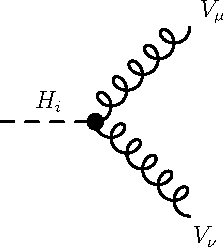
\includegraphics[height=3cm]{feyn_diagrams/diagrams/couplingHVV.pdf}
     }	\hspace{0.5cm}
     \subfigure[]{		
            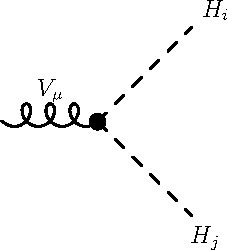
\includegraphics[height=3cm]{feyn_diagrams/diagrams/couplingVHH.pdf}
     }	\hspace{0.5cm}
     \subfigure[]{		
            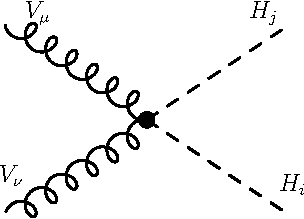
\includegraphics[height=3cm]{feyn_diagrams/diagrams/couplingVVHH.pdf}
     }
     \end{center}
   \label{fig:couplings}
    \caption{Feynman diagrams for the couplings between one Higgs boson and two gauge bosons (a), two Higgs bosons and one gauge boson (b)
		and two Higgs bosons and two gauge bosons (c). Based on~\cite{Djuadi}. }
\end{figure}
Among all of them, the most relevant for MSSM Higgs phenomenology are the trilinear couplings between two gauge bosons and one Higgs boson $V_{\mu}V_{\nu}H_i$.
For this case, since the photon is massless, there are no Higgs-$\gamma\gamma$ and Higgs-$Z\gamma$ couplings at tree level. CP-invariance also forbids $WWA$, $ZZA$
and $WZH^{\pm}$ couplings. Then, for the $V_{\mu}V_{\nu}H_i$ couplings, only the following possibilities remains:
\begin{align} 
Z_{\mu}Z_{\nu} h ~ :  ~ & ig_z M_Z \sin(\beta -\alpha) g_{\mu\nu},  &  Z_{\mu}Z_{\nu} H ~ : ~  ~    & ig_z M_Z \cos(\beta -\alpha) g_{\mu\nu} \\
W_{\mu}^+W_{\nu}^- h ~: ~&  ig_w M_W \sin(\beta -\alpha) g_{\mu\nu},  &  W_{\mu}^+W_{\nu}^- H ~ : ~ ~ & ig_w M_W \cos(\beta -\alpha) g_{\mu\nu} \label{eq:couplings} 
\end{align}
The couplings of the neutral CP-even Higgs bosons $h$ and $H$ with pair of vector bosons are proportional to $ \sin(\beta -\alpha)$ and $\cos(\beta -\alpha)$
respectively, where $\cos(\beta -\alpha)$ is fixed at tree level following equation~\eqref{eq:mixing}. An interesting phenomenological consequence is
that, calling $G_{VVh}$ and $G_{VVH}$ the coupling between two generic vector bosons and one of the neutral CP-even Higgs bosons the following equation holds:
\begin{equation}\label{eq:couplingSM}
G^2_{VVh} +G^2_{VVH} = g^2_{VVH_{SM}}
\end{equation}
The equations~\eqref{eq:couplings} and~\eqref{eq:couplingSM} leads to the fact that the couplings with vector bosons for $h$ ($H$) 
increase (decrease) with $\tan\beta$. For relatively large value of $\tan\beta$, $h$ has SM-like couplings with vector bosons while
 $H$  decouple from them. For an overview of all the other
couplings between vector bosons and Higgs bosons, charged Higgs, trilinear and quartic coupling between Higgs bosons and couplings 
to SUSY particles refer to Reference~\cite{Djuadi}.

The MSSM Higgs bosons couplings with isospin up-type $u$, and down-type $d$ fermions also depend on $\tan\beta$ and may be written
as follows:
\begin{small}
\begin{align*}
G_{huu} ~\propto ~ & m_u [\sin(\beta - \alpha)  + \cot\beta \cos(\beta - \alpha)], & G_{hdd} ~\propto ~ & m_u [\sin(\beta - \alpha)  - \tan\beta \cos(\beta - \alpha)]\\
G_{Huu} ~\propto ~& m_u [\cos(\beta - \alpha)  - \cot\beta \sin(\beta - \alpha)], & G_{Hdd} ~\propto~  & m_d [\cos(\beta - \alpha)  + \tan\beta \sin(\beta - \alpha)]\\
G_{Auu} ~ \propto ~ & m_u  \cot\beta, & G_{Add} ~ \propto ~ & m_d \tan\beta 
\end{align*} 
\end{small}
The couplings with down-type (up-type) fermions of either the $h$ or $H$ boson is enhanced (suppressed) by a factor $\tan\beta$, depending
on the magnitude of $\cos(\beta - \alpha)$ or $\sin(\beta - \alpha)$, while the coupling of $A$ boson with down-type (up-type) fermions are directly 
enhanced (suppressed) by $\tan\beta$.


\subsection{MSSM Higgs Benchmark Scenarios} \label{sec:benchmark}
At tree level, the MSSM  Higgs bosons masses, decay branching fraction and production cross section are all determined by two parameters,
by convention chosen to be $M_A$ and $\tan\beta$. As it has been pointed out in Section~\ref{sec:hsector}, radiative corrections
contribute significantly to the MSSM Higgs bosons masses and the prediction of physics observables becomes 
dependent on several MSSM parameters~\cite{Higgsm5}.
The main corrections arises from the top-stop (s)quark sector and for large $\tan\beta$ also the bottom-sbottom (s)quark sector becomes increasingly 
important. Furthermore, these corrections are dependent on the SUSY-breaking scale $M_{SUSY}$, the trilinear Higgs-stop, 
Higgs-sbottom Yukawa couplings, the electroweak gaugino and gluino mass parameters.

Due to the large number of free parameters, a complete scan of the MSSM parameter space is impractical in experimental analysis and phenomenological
studies. To cope with this difficulty several benchmark scenarios has been proposed~\cite{LHCxsec,mhmax2}, where the SUSY parameters
 entering via radiative corrections 
are fixed to particular benchmark values which exhibit interesting features of the MSSM Higgs phenomenology, while the parameters 
$M_A$ and $\tan\beta$ are left free to vary. Usually results are presented in a $M_A-\tan\beta$ plane.

The $m_h^{max}$ benchmark scenario~\cite{MSSMmhmax} was  used in the past searches for neutral MSSM Higgs bosons performed
at LEP, Tevatron and LHC~\cite{LEPLimits,TevatronLimits1,CMSLimit,ATLASLimit}. 
In this benchmark scenario the parameters that contributes to 
radiative corrections are fixed such that the mass of the light CP-even Higgs boson, 
$M_h$, is maximal under the variation of $M_A$ and $\tan\beta$. The $m_h^{max}$ scenario allows to set conservative 
lower bounds on $M_A$, $M_H^{\pm}$ and $\tan\beta$~\cite{mhmax2}. However, given the recent discovery of a Higgs
boson with mass $\sim 126$ GeV, this scenario
tend to predict a too high mass for $M_h$, resulting to be, for large regions of the MSSM parameter space, 
inconsistent with this observation. This scenario is still currently used in the presented analysis since it offer the possibility to
compare results with past experiments. 

Recently, several benchmark scenarios has been updated~\cite{LHCxsec} to  
accommodate the experimental constraints on past neutral MSSM Higgs searches and the observation of a SM-like Higgs boson.
An interesting updated benchmark scenario is the $m_h^{mod}$ scenario, which has the feature to predict $M_h \simeq 125.5 \pm 3 $ GeV 
for large region of MSSM parameter space.  The $m_h^{mod}$ scenario configuration is obtained by reducing the amount 
of mixing in the stop sector with respect to  the  $m_h^{max}$ scenario. This can be done for both signs of the MSSM parameter that 
regulate the stop mixing $X_t$, giving rise to two complementary scenarios $m_h^{mod+}$ and $m_h^{mod-}$.
The difference between these two scenarios is found to be negligible for experimental searches, the $m_h^{mod+}$ 
benchmark scenario has been used throughout this thesis as reference scenario.

Other interesting benchmark scenario are the light stop scenario and the light stau scenario.
The first may lead to relevant modification of the gluon fusion production cross section, while the second leads
to modification of the di-photon decay branching fraction of the light CP-even MSSM Higgs boson.
For an overview of other relevant  benchmark scenarios refer to Reference~\cite{LHCxsec}. 



 


\subsection{Neutral MSSM Higgs Bosons Production and Decay at LHC}
For large region of the MSSM parameter space a SM-like Higgs boson is expected, 
this role is commonly played by the lightest CP-even Higgs boson, $h$. 
Given the Higgs bosons couplings discussed in Section~\ref{sec:couplings} turns out that the MSSM Higgs bosons $H$ and $A$
tend to be degenerate in mass and decouple from gauge bosons. Furthermore the coupling of the latter
two Higgs bosons with down (up) type fermions are enhanced (suppressed) by $\tan\beta$, therefore, for large $\tan\beta$
bottom-quark and $\tau$ lepton will play an important role for 
the Higgs bosons production and its decays.  

The production of the neutral $CP$-even MSSM Higgs bosons at hadron
colliders proceeds via the same processes as for the SM Higgs
production. The pseudoscalar $A$, instead, cannot be produced
in association with gauge bosons or in vector boson fusion (VBF) processes at
tree-level, as this coupling is forbidden due to $CP$-invariance.  At
the LHC one of the most relevant production mechanisms for the MSSM
Higgs bosons is gluon fusion, $gg\rightarrow A/H/h$. In
addition, the production in association with $b$-quarks becomes
important for large value of $\tan\beta$. These are the only two production mechanism
that are considered in the presented analysis. Figure~\ref{fig:prod} shows the Feynman-diagram
for these processes, while Figure~\ref{fig:xsec} shows the production cross section of the neutral 
MSSM Higgs bosons via these two processes in the $m_h^{max}$ scenario.


The decays of the neutral
MSSM Higgs bosons (in the assumption that all supersymmetric particle
are heavy enough) are the same as for the SM one with the already
cited exception of $A$. Figure~\ref{fig:xsec} shows the decay branching fractions in the $m_h^{mod+}$ scenario
for $h$, $H$ and $A$ as a function of the mass of $A$ for two values of $\tan \beta$. The decay into tau lepton 
pairs is the most important after $b\bar{b}$ and the one used in this thesis. 

\begin{figure}[tp]
     \begin{center}
     \subfigure[]{		
            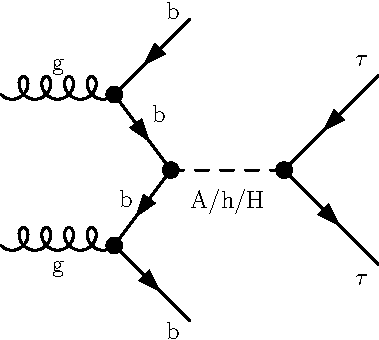
\includegraphics[height=3.5cm]{feyn_diagrams/diagrams/bbA.pdf}
     }\hspace{0.2cm}	
     \subfigure[]{		
            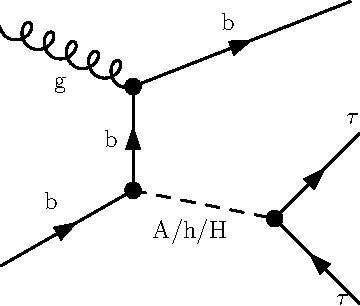
\includegraphics[height=3.5cm]{feyn_diagrams/diagrams/bbA2.pdf}
     }	\hspace{0.2cm}	
     \subfigure[]{		
            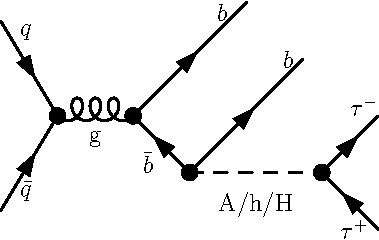
\includegraphics[height=3cm]{feyn_diagrams/diagrams/bbA3.pdf}
     }
     \subfigure[]{	
            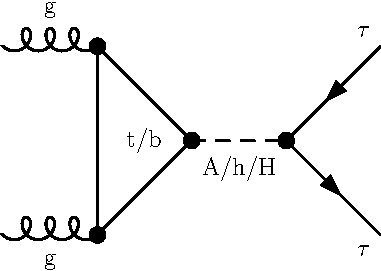
\includegraphics[height=3cm]{feyn_diagrams/diagrams/ggH.pdf}
	}	
     \end{center}
    \caption{Feynman diagram for the production of the neutral MSSM Higgs bosons in association with  $b$-quarks (a,b,c) and via gluon fusion (d) 
	processes, subsequent decay in tau lepton pairs is considered.}
   \label{fig:prod}
\end{figure}

\begin{figure}[tp]
     \begin{center}

     \subfigure[]{		
            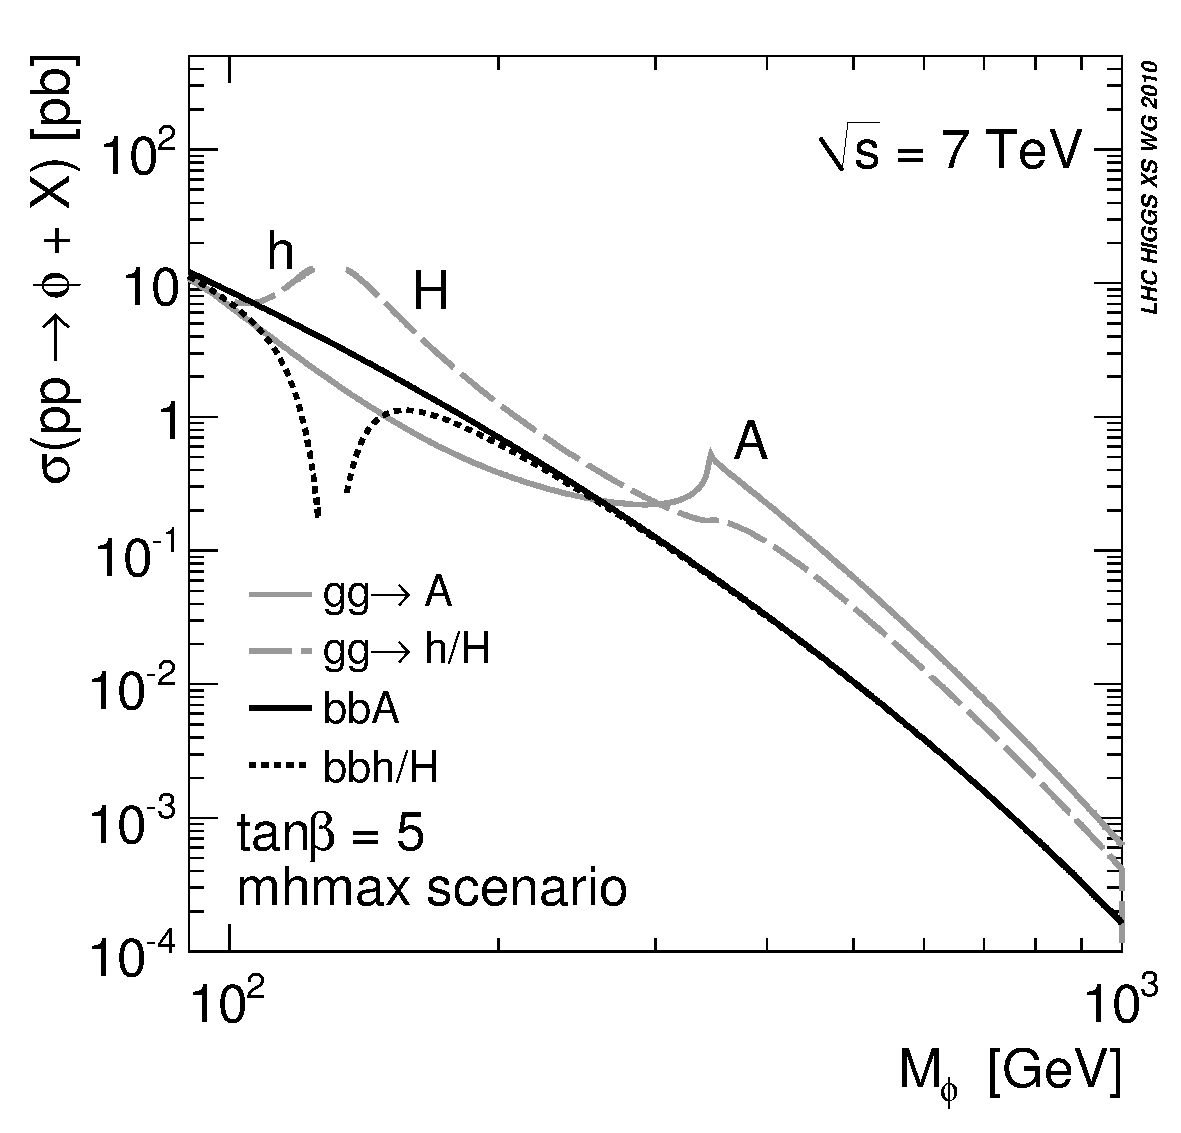
\includegraphics[width=0.6\textwidth]{figure/Xsec/YRHXS_MSSM_neutral_fig6a.pdf}
	}
     \subfigure[]{		
            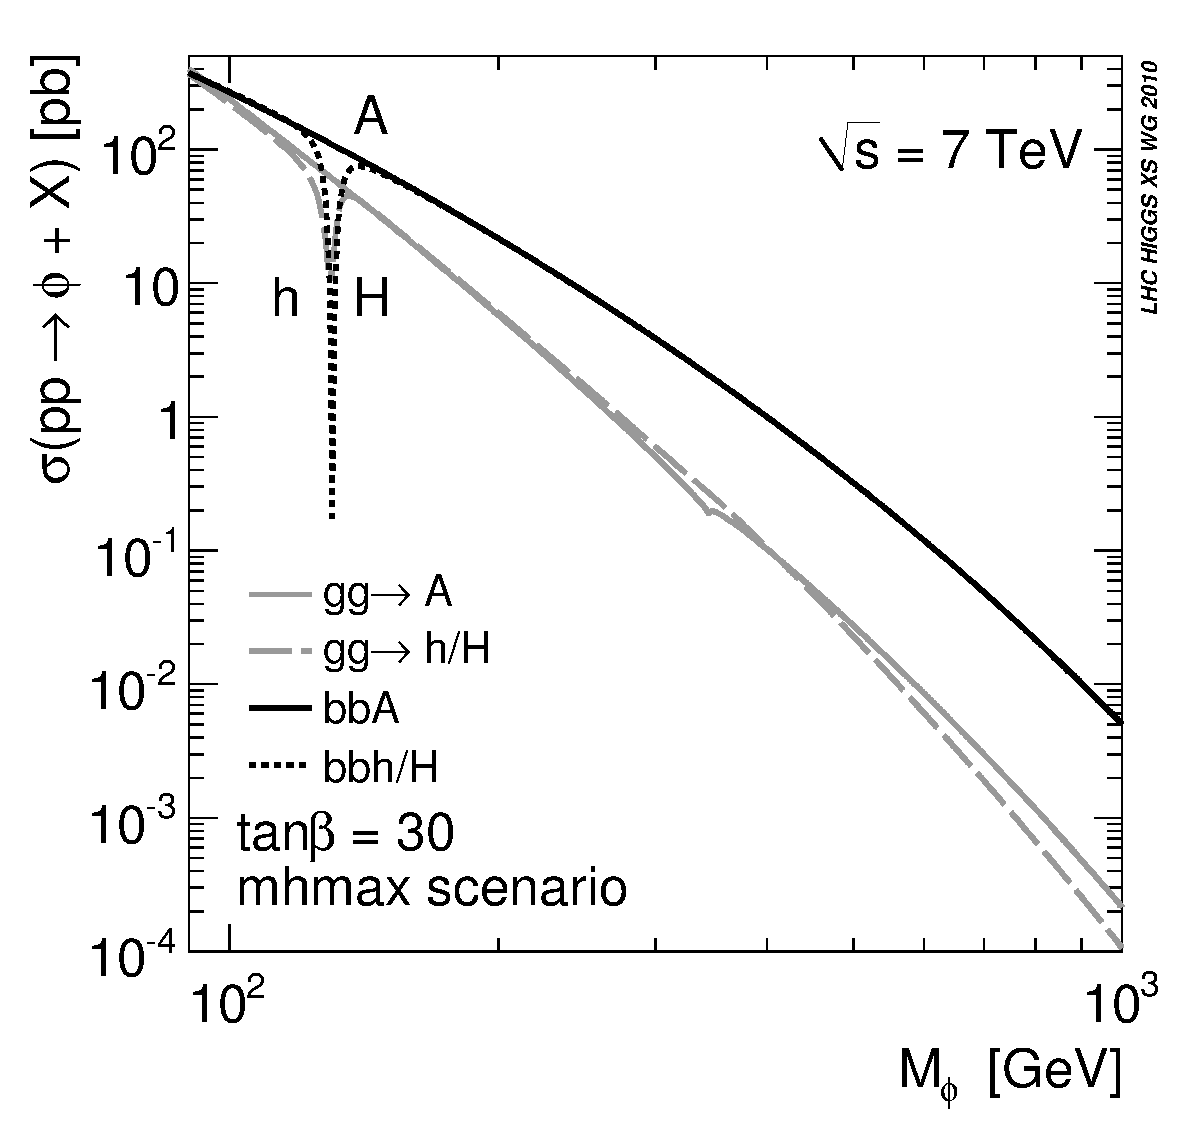
\includegraphics[width=0.6\textwidth]{figure/Xsec/YRHXS_MSSM_neutral_fig6b.pdf}
	}
    \end{center}
    \caption{Central predictions for the total MSSM Higgs bosons production cross sections via gluon fusion and Higgs radiation off
	bottom quarks  for $\sqrt{s} = 7$ TeV using NNLO and NLO MSTW2008 PDFs $m_h^{max}$ scenario; (a) $\tan\beta  = 5$, (b) $\tan\beta  = 30$.
	Reference~\cite{LHCxsec1}. }

   \label{fig:xsec}
\end{figure}


\begin{figure}[tp]
     \begin{center}

            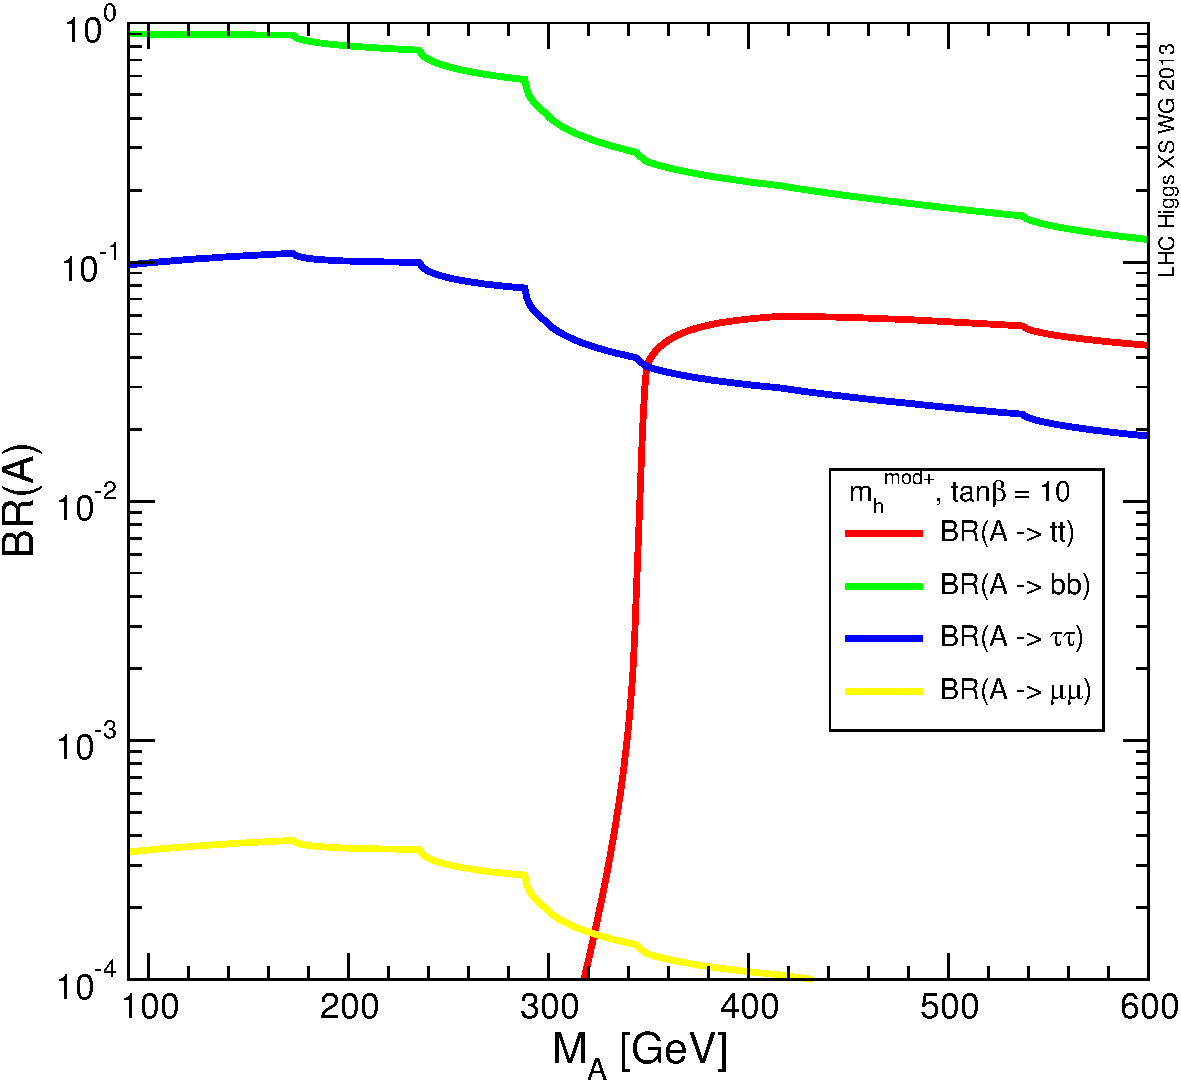
\includegraphics[width=0.47\textwidth]{figure/BR_higgs/YRHXS3_BR_fig31.pdf}
            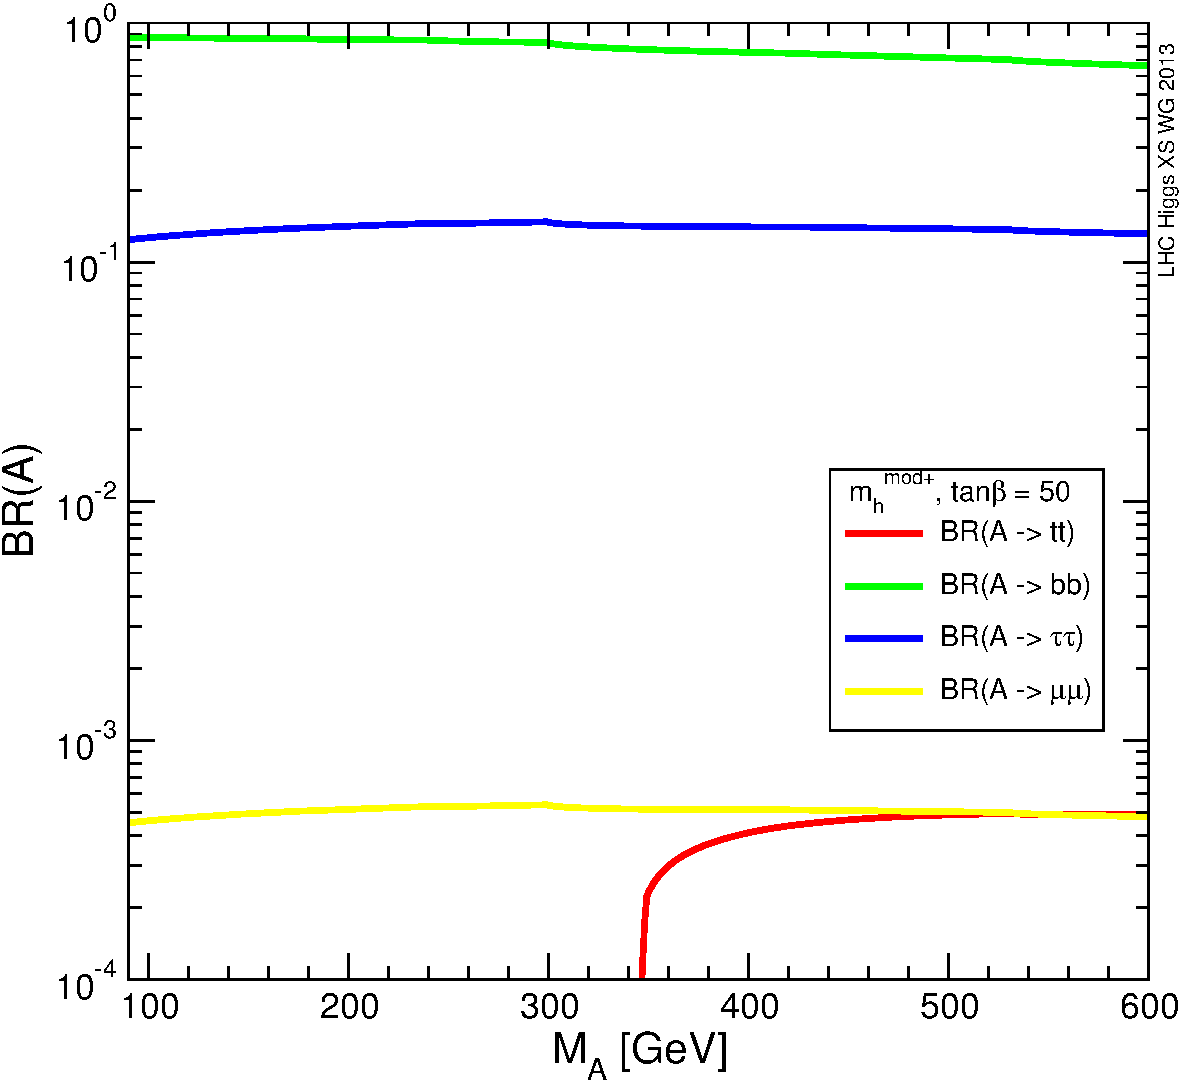
\includegraphics[width=0.47\textwidth]{figure/BR_higgs/YRHXS3_BR_fig32.pdf}
            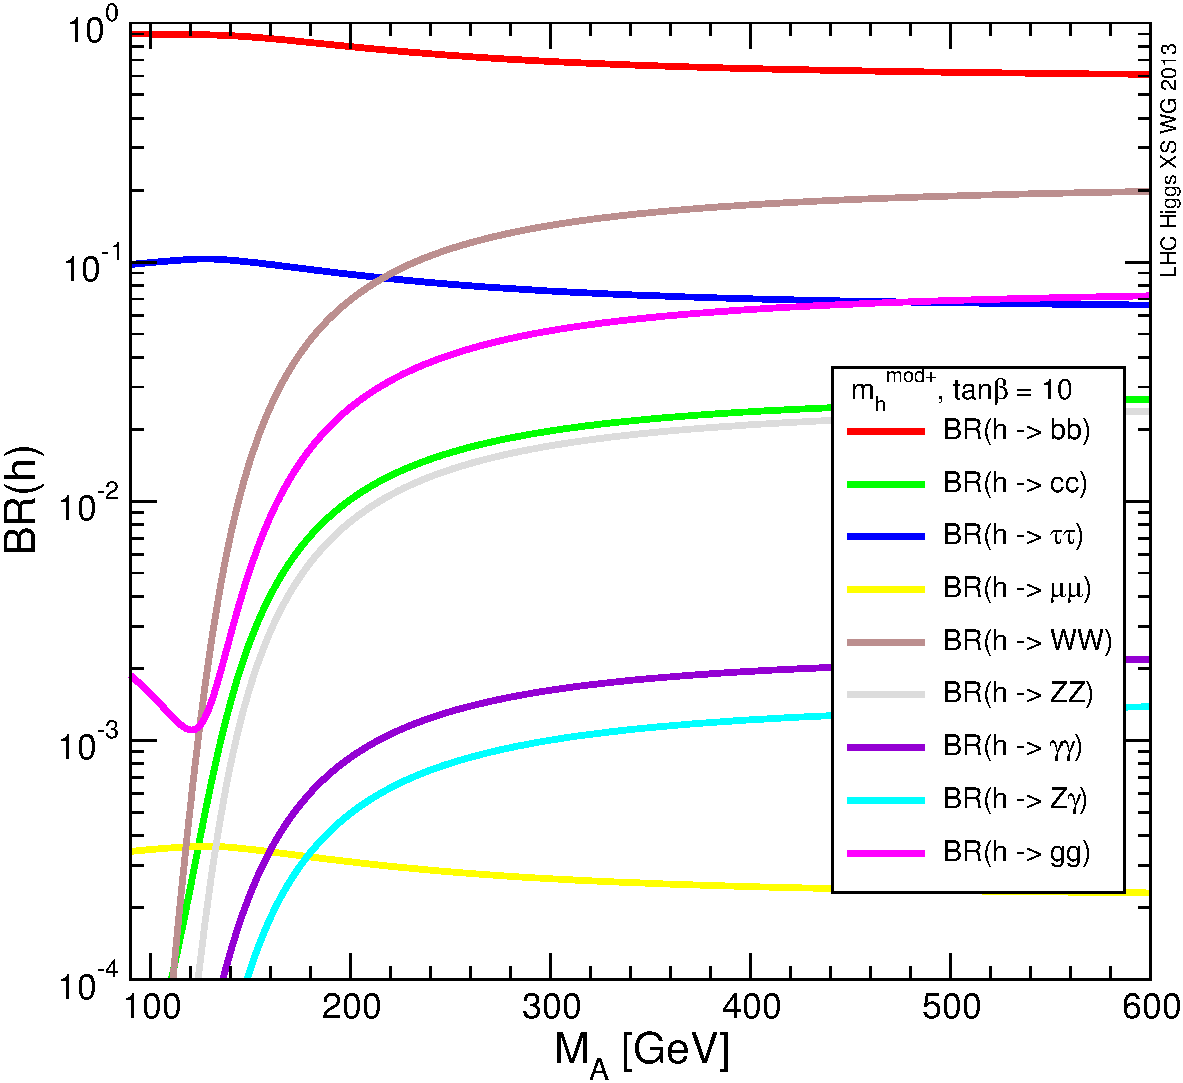
\includegraphics[width=0.47\textwidth]{figure/BR_higgs/YRHXS3_BR_fig35.pdf}
            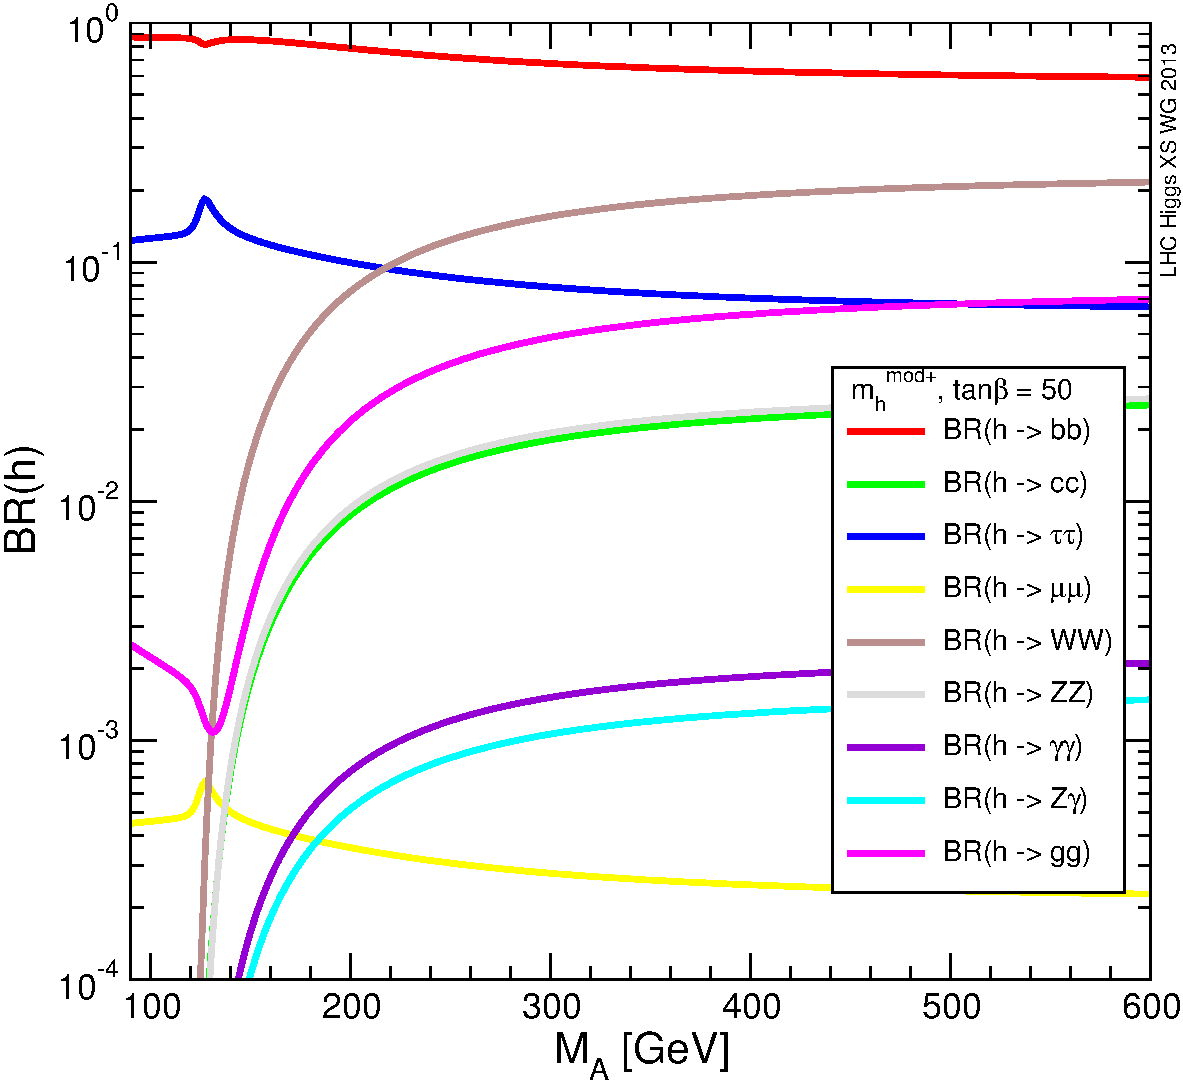
\includegraphics[width=0.47\textwidth]{figure/BR_higgs/YRHXS3_BR_fig36.pdf}
            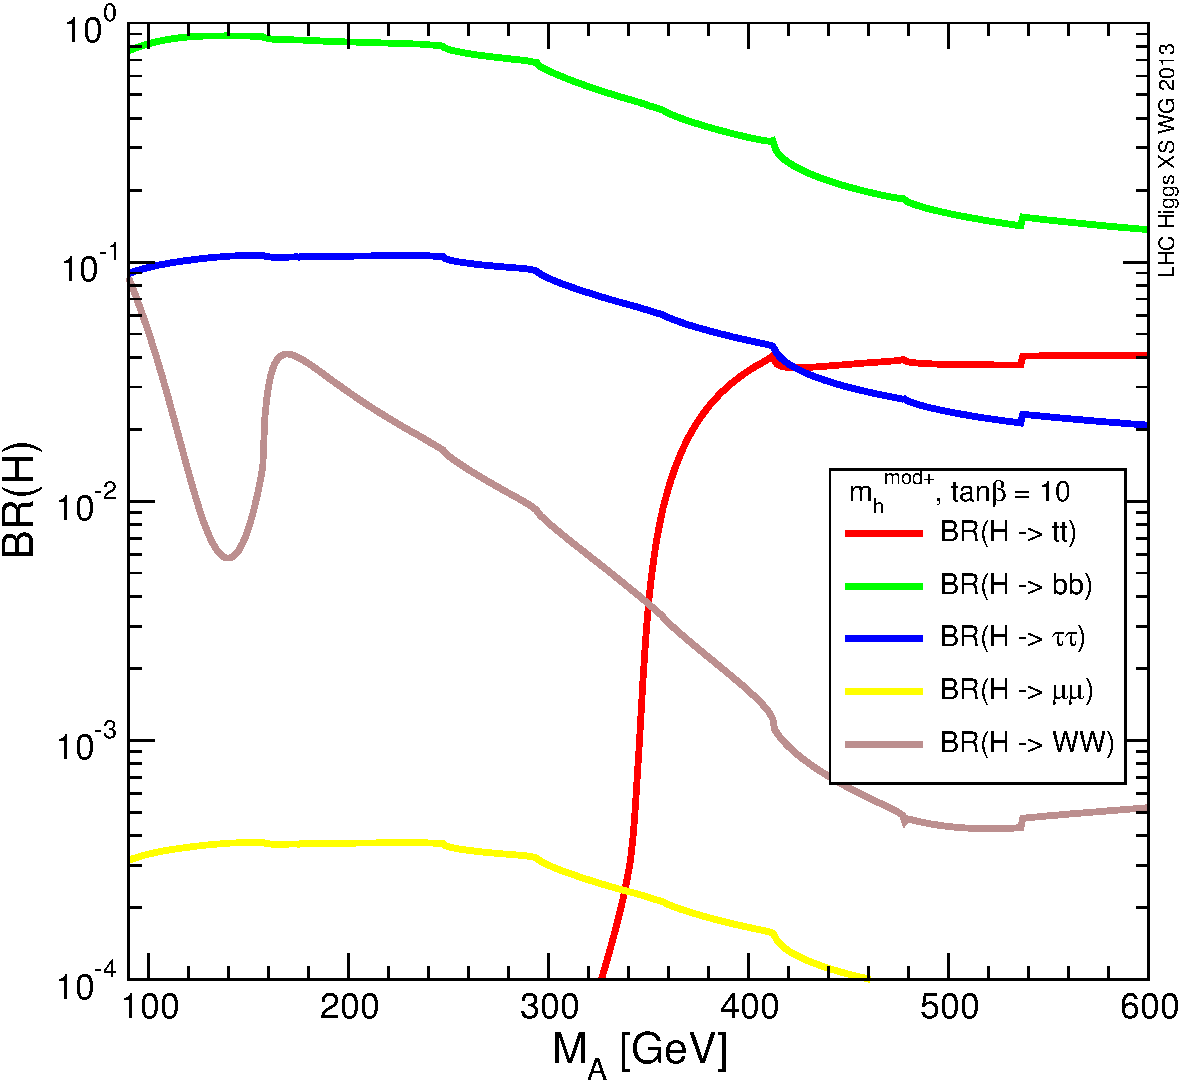
\includegraphics[width=0.47\textwidth]{figure/BR_higgs/YRHXS3_BR_fig37.pdf}
            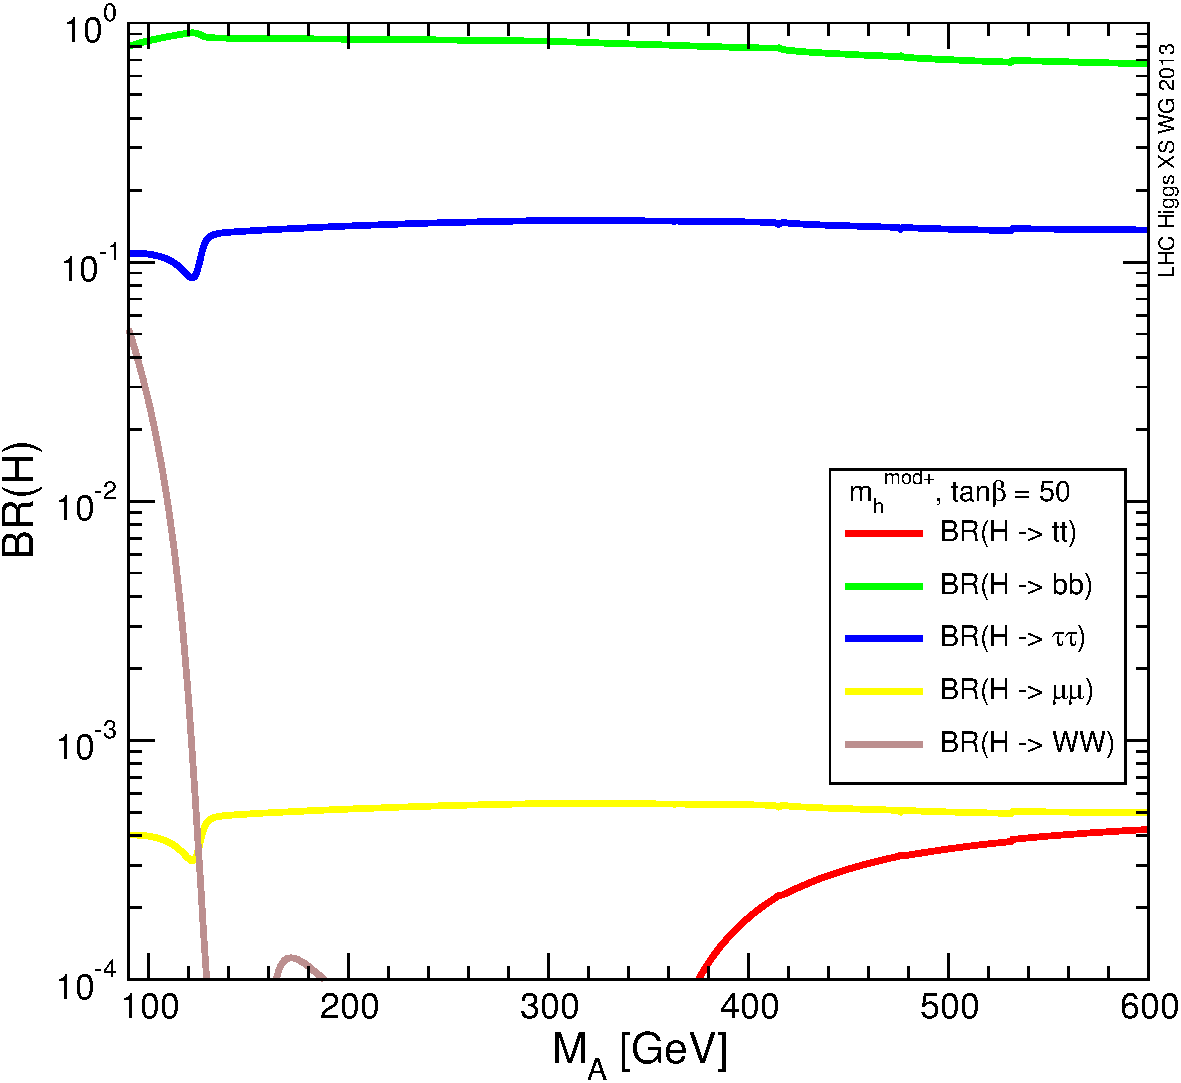
\includegraphics[width=0.47\textwidth]{figure/BR_higgs/YRHXS3_BR_fig38.pdf}

    \end{center}
    \caption{Branching fraction for the MSSM neutral Higgs bosons, $h/H/A$, in the $m_h^{mod+}$ scenario for $\tan\beta=10$ and
	$\tan\beta=50$. Reference~\cite{LHCxsec}.}
   \label{fig:br}

\end{figure}



\subsection{Current Status of the Search for Neutral MSSM Higgs Bosons}

The measure of the couplings of the observed SM-like Higgs boson can shed light on the Higgs sector and determine if this boson
is fully responsible for the generation of all the SM particles masses. 
%In fact, the couplings are sensitive to new physics,
%given the unitarity property of scattering amplitudes for longitudinal vectors and fermions, 
There are two approaches to explore the Higgs sector: one, is to use the measured Higgs couplings with SM particles to 
set constraint on new physics, while the other is to directly search for additional Higgs bosons in a well defined model.

In case the SM-like Higgs boson is interpreted as the light CP-even Higgs boson of the MSSM, the couplings of the Higgs boson 
to vector bosons ($k_V$), up-type fermions ($k_u$) and down-type fermions ($k_d$), can be expressed as a function of  $m_A $ and $\tan\beta$ 
and this allow to set exclusion limits in the $m_A - \tan\beta$ plane~\cite{AtlasConstraint}. Figure~\ref{fig:ex1} shows the exclusion limits in a 
``simplified MSSM'' model~\cite{sympleMSSM1,sympleMSSM2} via fits to the measured rates of Higgs boson production and decay.

 
\begin{figure}[tp]
     \begin{center}

            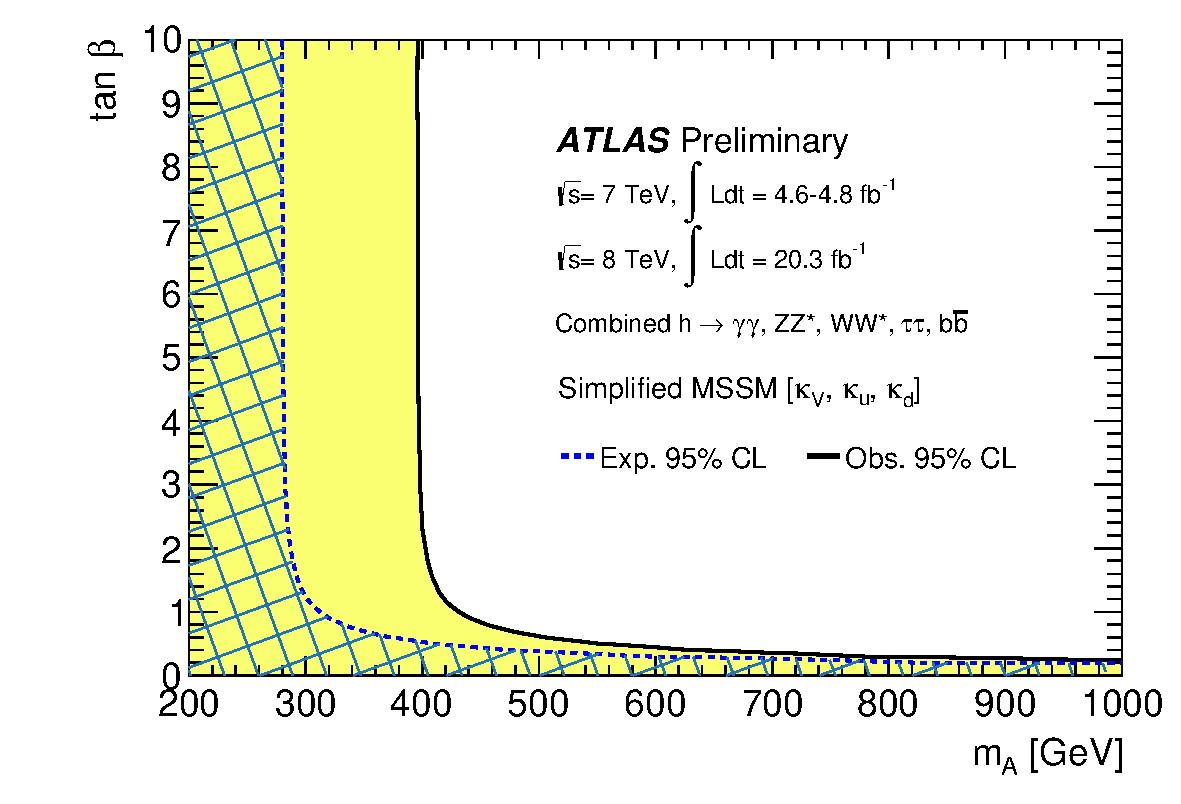
\includegraphics[width=0.8\textwidth]{figure/limits/constraintAtlas.pdf}

    \end{center}
    \caption{Regions of the  $m_A - \tan\beta$ plane excluded in a simplified MSSM model via fits to the measured
rates of Higgs boson production and decays. The likelihood contours where $−2 \ln \Lambda = 6.0$, corresponding
approximately to 95\% CL ($2\sigma$), are indicated for the data and expectation assuming the SM Higgs sector.
The light shaded and hashed regions indicate the observed and expected exclusions, respectively. The
SM decoupling limit is $m_A \rightarrow \infty$. See Reference~\cite{AtlasConstraint}.}

   \label{fig:ex1}
\end{figure}


The current latest constraint on $m_A - \tan\beta$  by direct search of neutral MSSM Higgs bosons~\cite{} are  shown in Figure~\ref{fig:ex2}
and are part of the work of this thesis.



 
\begin{figure}[tp]
     \begin{center}

            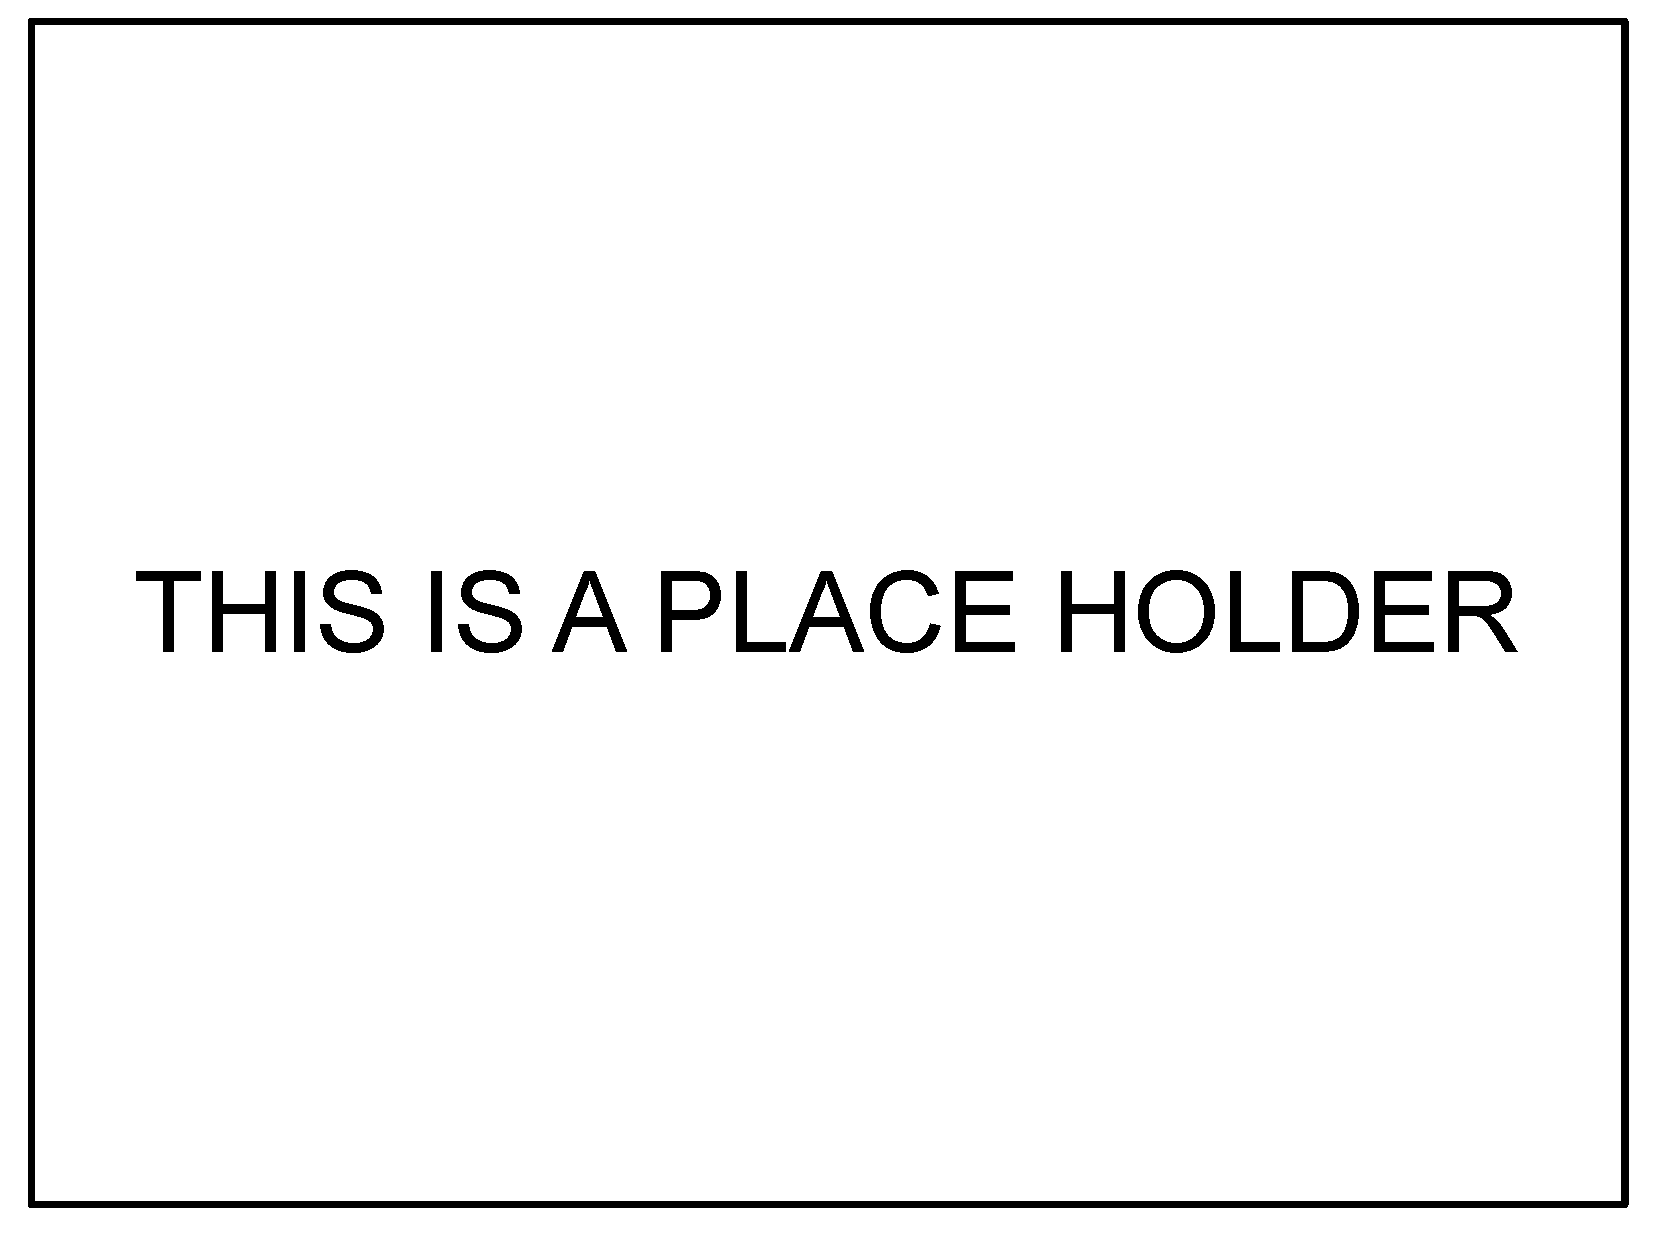
\includegraphics[width=0.8\textwidth]{figure/blank.pdf}

    \end{center}
    \caption{Limit CMS or ATLAS depending if we manage to publish in time}


   \label{fig:ex2}
\end{figure}





















%\chapter{Theory}
\section{Higgs Phenomenology}

The Higgs sector of the Minimal Supersymmetric Standard Model (MSSM) consists of two SU (2) dou-
blets, H1 and H2 , whose relative contribution to electroweak symmetry breaking is determined by the
ratio of vacuum expectation values of their neutral components, tan β ≡ v2 /v1 . The spectrum of phys-
ical Higgs bosons is richer than in the SM, consisting of two neutral scalars h and H, one neutral pseu-
doscalar, A, and two charged scalars, H±. At the tree level, the mass matrix for the neutral scalars can be
expressed in terms of the parameters MZ , MA and tan β, and the mass of the lightest scalar h is bounded
from above by MZ . However, radiative corrections – especially those involving top and bottom quarks
and their supersymmetric partners, the stop and sbottom squarks – can significantly alter the tree-level
predictions for the Higgs-boson masses, and bring along a dependence on a large number of free pa-
rameters of the MSSM. While the CP symmetry is conserved at tree level in the MSSM Higgs sector,
radiative corrections can also introduce CP-violating phases, and induce mixing among all three neutral
states. In this report, however, we will focus on the CP-conserving case, by considering only real values
for the parameters in the soft SUSY-breaking Lagrangian and for the Higgs mass μ in the superpotential.
In general, the couplings of the MSSM Higgs bosons to gauge bosons and matter fermions dif-
fer from those of the SM Higgs. However, in large regions of the MSSM parameter space one of the
scalars has SM-like couplings, while the other Higgs bosons are decoupled from the gauge bosons, and
their couplings to down-type (up-type) fermions are enhanced (suppressed) by tan β. As in the SM,
gluon fusion is one of the most important production mechanisms for the neutral Higgs bosons, whose
couplings to the gluons are mediated by the top and bottom quarks and their superpartners. However,
for intermediate to large values of tan β the associated production with bottom quarks can become the
dominant production mechanism for the neutral Higgs bosons that have enhanced couplings to down-
type fermions. The production of the charged Higgs H±, on the other hand, proceeds mainly through
its coupling to a top-bottom pair. A sufficiently light H± is produced in the decay of a top quark, and it
decays dominantly in a tau-neutrino pair. A heavy H± is produced in association with a top quark and it
decays dominantly in a top-bottom pair.
The discovery by ATLAS and CMS of what appears to be a neutral scalar with mass around
125.5 GeV [1, 2] puts the studies of the Higgs sector of the MSSM in an entirely new perspective. In
order to remain viable, a point in the MSSM parameter space must now not only pass all the (ever
stricter) experimental bounds on superparticle masses, but also lead to the prediction of a scalar with
mass, production cross section and decay rates compatible with those measured at the LHC. In particular,
the relatively large mass of the roughly-SM-like scalar discovered at the LHC implies either very heavy
stops, of the order of 3 TeV, or a large value of the left-right stop mixing term (see, e.g., Refs. [648,649]).
The “benchmark scenarios” routinely considered in MSSM studies had been devised when the Higgs
sector was constrained only by the LEP searches, and many of them, such as the so-called “no-mixing”
scenario, are now ruled out because they predict a too-light SM-like scalar. Others, such as the so-called
mmax scenario, are constrained for the opposite reason, i.e. they can predict a too-heavy SM-like scalar.
h
To address the need for new benchmark scenarios to be used in future studies of the MSSM Higgs sector,
in Section 14.2 we will define scenarios that are compatible both with the properties of the Higgs boson
discovered at the LHC and with the current bounds on superparticle masses.
The fact that information on the Higgs boson mass, production and decays has now become avail-
able also puts new emphasis on the need for accurate theoretical predictions of those quantities. In the
studies presented in this report, the masses and mixing of the MSSM Higgs bosons are computed with
the public code F EYN H IGGS [24–27], which implements the full one-loop radiative corrections together
with the dominant two-loop effects. The theoretical accuracy of the prediction of F EYN H IGGS for the

lightest-scalar mass was estimated to be of the order of 3 GeV [26, 650, 651], i.e., already comparable
to the accuracy of the mass measurement at the LHC. Improving the accuracy of the theoretical predic-
tion for the MSSM Higgs masses will require the inclusion in public computer codes of the remaining
two-loop effects [652–654] and at least the dominant three-loop effects [655–657].
The production and decay rates of a SM-like Higgs boson in the MSSM are sensitive to contri-
butions from virtual SUSY particles, and their measurement at the LHC – combined with the searches
for additional Higgs bosons – can be used to constrain the MSSM parameter space. To this effect, the
theoretical predictions for cross section and decays must include precise computations of the SUSY con-
tributions. In Section 14.3 we use the public code S US H I [641] and the POWHEG implementation of
Ref. [77] to compute the total and differential cross sections for neutral Higgs-boson production in gluon
fusion, including a NLO-QCD calculation of quark and squark contributions plus higher-order quark
contributions adapted from the SM calculation. We show that the SUSY contributions can be sizeable in
regions of the MSSM parameter space where the third-generation squarks are relatively light, and discuss
the theoretical uncertainty of the predictions for the cross sections.
Finally, we study and update the exclusion limits on light charged MSSM Higgs bosons in the
(MH± , tan β)-plane in various benchmark scenarios in Section 14.4. Particular emphasis is placed on
the dependence of the limits on the variation of SUSY parameters. We also provide improved NLO-
QCD cross section predictions for heavy charged Higgs production in the so-called four and five-flavor
schemes in Section 14.5. The five-flavor scheme cross section is calculated with a new scheme for setting
the factorization scale and takes into account the theoretical uncertainty from scale variation and the PDF,
αs and bottom-mass error. We observe good agreement between the 4FS and 5FS NLO-calculations and
provide a combined prediction following the Santander matching.
14.2
New MSSM benchmark scenarios
Within the MSSM an obvious possibility is to interpret the new state at about 125.5 GeV as the light
CP-even Higgs boson [334, 338, 648, 649, 658–662]. At the same time, the search for the other Higgs
bosons has continued. The non-observation of any additional state in the other Higgs search channels
puts by now stringent constraints on the MSSM parameter space, in particular on the values of the tree-
level parameters MA (or MH± ) and tan β. Similarly, the non-observation of supersymmetric (SUSY)
particles puts relevant constraints on the masses of the first and second generation scalar quarks and the
gluino, and to lesser degree on the stop and sbottom masses (see Refs. [663, 664] for a recent summary).
Due to the large number of free parameters, a complete scan of the MSSM parameter space is
impractical in experimental analyses and phenomenological studies. Therefore, the Higgs search results
at LEP were interpreted [458] in several benchmark scenarios [16, 665]. In these scenarios only the two
parameters that enter the Higgs sector tree-level predictions, MA and tan β, are varied (and the results are
usually displayed in the MA − tan β plane), whereas the other SUSY parameters, entering via radiative
corrections, are fixed to particular benchmark values which are chosen to exhibit certain features of the
MSSM Higgs phenomenology. These scenarios were also employed for the MSSM Higgs searches at
the Tevatron and at the LHC.
By now, most of the parameter space of the original benchmark scenarios [16, 665] has been
ruled out by the requirement that one of the CP-even Higgs boson masses should be around 125.5 GeV.
Consequently, new scenarios have been proposed [31], which are defined such that over large parts of
their available parameter space the observed signal at about 125.5 GeV can be interpreted in terms of
one of the (neutral) Higgs bosons, while the scenarios exhibit interesting phenomenology for the MSSM
Higgs sector. The benchmark scenarios are all specified using low-energy MSSM parameters, i.e. no
particular soft SUSY-breaking scenario was assumed. Constraints from direct searches for Higgs bosons
are taken into account, whereas indirect constraints from requiring the correct cold dark matter density,
BR(b → sγ), BR(Bs → μ+ μ− ) or (g−2)μ are neglected. However interesting, those constraints de

\begin{figure}[tp]
     \begin{center}

            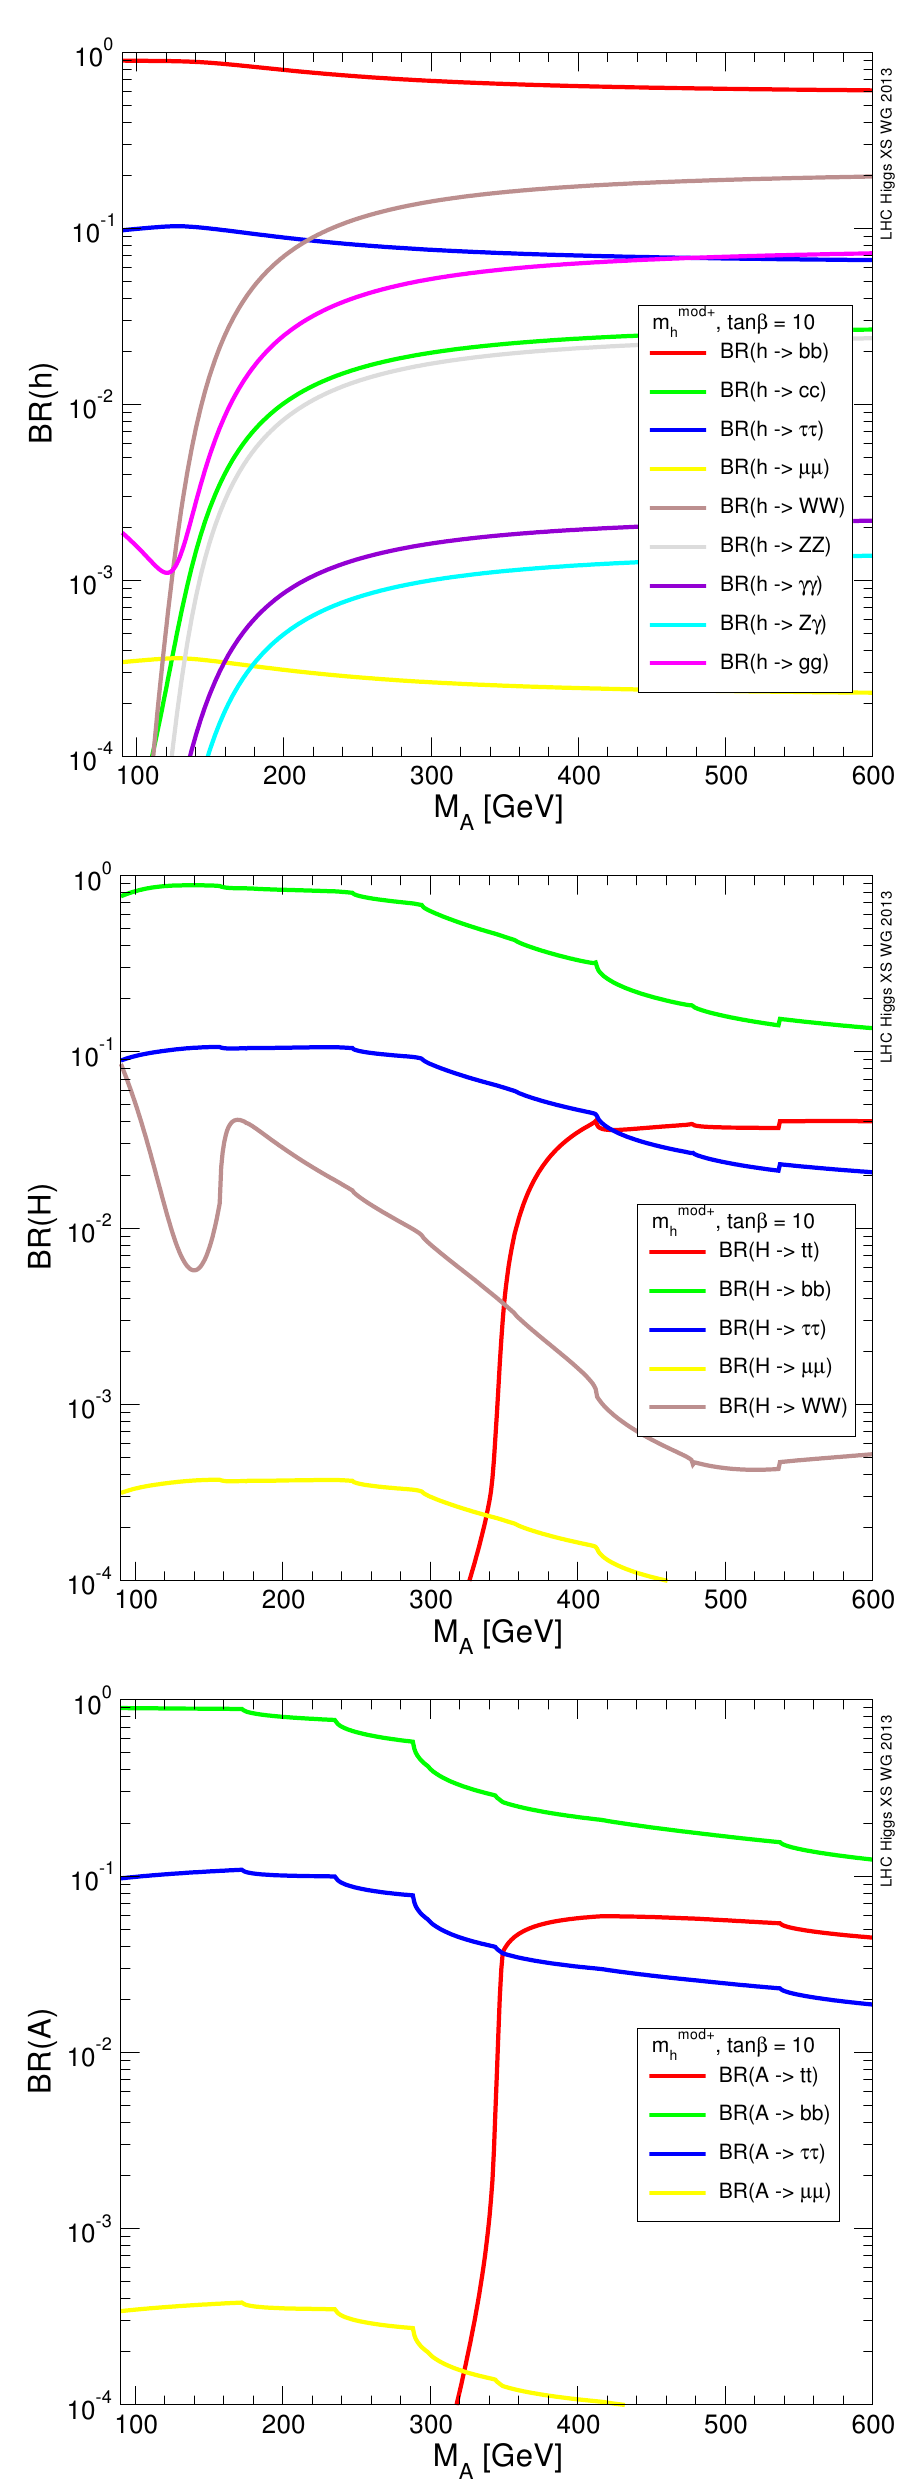
\includegraphics[width=0.5\textwidth]{figure/br.png}

    \end{center}
    \caption{Branching fraction for the MSSM neutral higgses $h/H/A$ in the $m_h^{mod+}$ scenario.}
   \label{fig:br}

\end{figure}



\chapter{LHC and The ATLAS Detector}
%%%%%%%%%%%%%%%%%%%%  questa parte va nel detector chapter %%%%%%%%%%%%%%%%%%%%%%%%
%This problematic has two sources:
%- The ATLAS calorimeter is not a sampling calorimeter, this means that responses differently 
%for Hadrons and for leptons, has different responses to electromagnetic and hadronic shower.
%The Calorimeter cells are calibrated in energy using response to electromagnetic showers, to 
%know the energy of the original parton that initiated the jet there are different procedure 
%to calibrate the Jets offline which are called in short Jet Energy Scale (JES) corrections \cite{}, 
%which make use of MC simulation.
%%%%%%%%%%%%%%%%%%%%%%%%%%%%%%%%%%%%%%%%%%%%%%%%%%%%%%%%%%%%%%%%%%%%%%%%%%%%%%%%%%%%

\chapter{Reconstruction of Physics Object}\label{chap:obj}
\vspace{3cm}
To allow the use of all the information enclosed in a bunch crossing, the collection
of all ATLAS detector signals needs to be translated in more user friendly object, 
the reconstruction of the event is carryed out by the ATLAS event reconstruction 
software framework ATHENA~\cite{Athena}. 

Physical particle like electron, muons, hadronic jets, ecc, are all described by means 
of off line software reconstructed object. In section~\ref{} the electron reconstuction 
algorithm is briefly described,
for more details on reconstructed object and their performance see~\cite{AtlasCSCBook}

%In this section the preselection and reconstruction criteria for the
%objects used in this analysis are presented.  For each object and
%selection criteria all corrections that have been applied to data and
%MC are also described.  A summary of the preselection on physics
%objects used in this analysis is reported in Table~\ref{tab:presel}.
\clearpage

\section{Tracks and Vertex Reconstruction}
The reconstruction of charged particles tracks and interaction vertex is based on Inner Detector
information, charged particle bends in the transverse plane due to the magnetic field of the Inner Detector and
this allow to measure their transverse momentum, they can only be reconstructed whithin $|\eta| < 2.5$.
To fully carachterize a track other parameters need to be measured
and those are: the $\phi$ and $\theta$ angles to define its direction, the impact parameter is the 
distance of clostest approach o the track to the beam axis calculated with respect to the origin of coordinate, $d_0$ 
is the impact parameter in the $x-y$ plane,  while $z_0$  is along the $z$ axis.
The transverse impact parameter $d_0$ is the distance of closest approach of the track to the primary vertex
point in the $r-\phi$ projection. The $z$ coordinate of the track at this point of closest approach is referred to $z_0$

\paragraph{Track Reconstruction}
Tracks are reconstructed  by the Inner Detector track reconstruction software~\cite{IDtracking}.
First raw data from the pixel and SCT detectors are transformed in three dimensional space points 
which are called ``hits'', while the  TRT detector information is translated into drift circles. 
Thn, track seeds are formed from a combination of space-points in the three pixel layers and the first SCT layer, these
seeds are then extended throughout the SCT to form track candidates. The tracks candidate are fitted 
using a \emph{Kalman filter} algorothm~\cite{Kalman}, ambiguities in the cluster-to-track association are resolved
and fake tracks are rejected. The selected tracks are then extended to the TRT and finally refitted with the full information of all three
detectors. To help improve tracking efficiency for secondary tracks coming from photon conversion or decays of long-lived 
particles (like kaons), a complementary algorithm searches foir unused track segments in the TRT, which will be then extended
towards the SCT and the pixel in a very similar way as described for the default algorithm.
All tracks found with $\pt > 100$ MeV are written to the database.

%Next, these candidates are
%fitted, “outlier” clusters are removed, ambiguities in the cluster-to-track association are resolved,
%and fake tracks are rejected. 
%
%Silicon pixel, stripes ecc.. responds to te passage of charged particle with a signal,
%those signal are interpreted on a boolean bases and are called ``hits'', 
%The inner detector track reconstruction software [5] follows a modular and flexible software design,
%%which includes features covering the requirements of both the inner detector and muon spectrometer [2]
%%reconstruction. These features comprise a common event data model [6] and detector description [7],
%%which allow for standardised interfaces to all reconstruction tools, such as track extrapolation, track fitting
%%including material corrections and vertex fitting. The extrapolation package combines propagation
%%tools with an accurate and optimised description of the active and passive material of the full detector [8]
%%to allow for material corrections in the reconstruction process. The suite of track-fitting tools includes
%%global-c2 and Kalman-filter techniques, and also more specialised fitters such as dynamic noise adjustment
%%(DNA) [9], Gaussian-sum filters (GSF) [10] and deterministic annealing filters [11]. Optimisation
%%of these tools continues and their performance will need to be evaluated on real data. The tools intended
%%to cope with electron bremsstrahlung (DNA and GSF – see Section 5.1) will be run after the track reconstruction,
%%as part of the electron-photon identification. Other common tracking tools are provided,
%%including those to apply calibration corrections at later stages of the pattern recognition, to correct for
%%module deformations or to resolve hit-association ambiguities.
%Track reconstruction in the inner detector is logically sub-divided into three stages:
%1. A pre-processing stage, in which the raw data from the pixel and SCT detectors are converted
%into clusters and the TRT raw timing information is translated into calibrated drift circles. The
%SCT clusters are transformed into space-points, using a combination of the cluster information
%from opposite sides of a SCT module.
%2. A track-finding stage, in which different tracking strategies [5, 12], optimised to cover different
%applications, are implemented. (The results of studies of the various algorithms are reported else-
%where [13].) 
%
%The default tracking exploits the high granularity of the pixel and SCT detectors to
%find prompt tracks originating from the vicinity of the interaction region. First, track seeds are
%formed from a combination of space-points in the three pixel layers and the first SCT layer. These
%seeds are then extended throughout the SCT to form track candidates. Next, these candidates are
%fitted, “outlier” clusters are removed, ambiguities in the cluster-to-track association are resolved,
%and fake tracks are rejected. This is achieved by applying quality cuts. For example, a cut is made
%on the number of associated clusters, with explicit limits set on the number of clusters shared between
%several tracks and the number of holes per track (a hole is defined as a silicon sensor crossed
%by a track without generating any associated cluster). The selected tracks are then extended into
%the TRT to associate drift-circle information in a road around the extrapolation and to resolve the
%left-right ambiguities. Finally, the extended tracks are refitted with the full information of all three
%detectors. The quality of the refitted tracks is compared to the silicon-only track candidates and
%hits on track extensions resulting in bad fits are labelled as outliers (they are kept as part of the
%track but are not included in the fit).
%A complementary track-finding strategy, called back-tracking, searches for unused track segments
%in the TRT. Such segments are extended into the SCT and pixel detectors to improve the tracking
%efficiency for secondary tracks from conversions or decays of long-lived particles.
%3. A post-processing stage, in which a dedicated vertex finder is used to reconstruct primary vertices.
%This is followed by algorithms dedicated to the reconstruction of photon conversions and of
%secondary vertices.

\paragraph{Vertex Reconstruction}
The vertex recostruction algorithm and its performance are described in full detail in~\cite{AtlasCSCBook,VertexPerf} and
only briefly summarized here.
%say good tracks
The vertex finding is perfomed as follows:  a set of well reconstructed tracks are selected,
a vertex is seeded according to the global maximum of the selected tracks $z$ coordinate distribution, the tracks $z$ coordinate 
is computed with respect the expected averange collision point. 
An adaptive vertex fitting algorithm~\cite{Vertex} determines the vertex position taking as input the vertex seed position and the 
tracks around it. Tracks that are incompatible with the found vertex by more than seven standard deviation
are used to seed the next vertex. The iteration continues untill no tracks are left or no additional vertex can be found.
The procedure depends  on the expected position of the averange interaction point, which is monitored 
during LHC data taking and is computed every few minutes with the method described in~\cite{beamspot}.

The vertex with the larger sum of tracks $\pt$ associated is identified as the \emph{primary vertex} (PV), 
i.e. the interaction point related to the hard scattering of the event. All the other vertices are assumed to result from
minimum bias interaction and are called \emph{pile-up} vertices.
In data recorded during 2012, an averange of 21 multiple interaction are occurred per bunch crossing,
such a high vertex multiplicity strongly affects the ambient energy density in the event, 
a correct pile-up description is then crucial for MC simulation. The ATLAS MC production assures that events 
are simulated with various pile-up conditions, simulated events are then weighted according to the averange interaction
per bunch crossing recorded in data.


\section{Jets Reconstruction and Energy Calibration}
Jets are reconstructed in ATLAS by means of the FastJet package~\cite{fastjet}, 
which provides a broad range of jet finding algorithms and analysis tools. 
In the following jet reconstruction methods relevant for the
analysis presented in this theses are brifly described, for more detail see~\cite{AtlasCSCBook}.

In general, jets may be reconstructed out of any set of four vector objects, 
however in ATLAS, the most important detectors for jet reconstruction are the ATLAS calorimeters.
Calorimeter cells are grouped togheter by a clustering algorithm forming what are called \emph{topological clusters}~\cite{TopoClusterAlgo},
those are three-dimensional cluster representing the energy deposition of the shower.
the clustering starts with seed cells with a signal-to-noise ratio greather that a certain threshold, 
all nearby cells are grouped to the seed cells if they passes a second, lower, signal-to-noise ratio treshould.

Topological clusters are then fed to an \emph{anti-$k_t$} algorithm~\cite{antikt}. The algorithm defines a metric
to assess distances between the clusters $i$ and $j$, the metric is defined as follows:
\begin{align}
d_{ij} &= \text{min}(\frac{1}{k_{t,i}^2}, \frac{1}{k_{t,j}^2}) \cdot \frac{\Delta R_{ij}^2}{R^2}  \\
d_i   &= \frac{1}{k_{t,i}^2} 
\end{align}
where $k_{t,i}$ is the $\pt$ of the cluster $i$ and $\Delta R_{ij}^2 = \sqrt{\Delta\phi_{ij}^2 + \Delta\eta_{ij}^2}$, for
this analysis $R=0.4$ is chosen.
If the distance between two cluster $d_{ij}$ is smaller that $d_i$ the clusters are grouped togheter and their four momentum
summed, otherwise their are kept as single entity. The clustering procedure is iterated until is not possible to merge object
anymore. The metric is designed in a way that high $\pt$ jet will accumulate the soft activity surrounding them leading to conical
jet shapes. 

Given the high pile-up environment of LHC  is important to distinguish jets coming from the hard scattering process and those
related to pile-up interaction, for this purpose a techique, called \emph{jet vertex fraction} (JVF), is implemented in the 
ATLAS jet reconstruction software.
The JVF relies on Inner Detector informations, it is defined as the $\pt$ weighted fraction of tracks pointing
to to the primary vertex associated to the jet:
\begin{equation}
\text{JVF} = \frac{\sum\limits_{PV-tracks}\pt}{\sum\limits_{tracks}\pt}
\end{equation} 
the jet vertex fraction  is only available within Inner Detector coverage $|\eta| < 2.5$,
while calorimeter jet reconstruction is possible up to $|\eta| < 4.5$.

\paragraph{Calorimeter Jet Energy Calibration}
The ATLAS calorimeters were calibrated using test beam electrons~\cite{EMcalibration}, however  the response
to electromagnetic shower  is different from the one to hadronic shower, a dedicated jet energy scale
(JES) calibration is then performed by means of MC simulation~\cite{jesinsitu}: 
jet energy is corrected to correspond, as a mean value, to the simulated energy 
of the hadronizing parton origin of the jet. The direction of the jet is also corrected to constraint it to point
to the primary vertex instead to the center of the ATLAS detector. A set of corrections are then evaluated to take into account
effect of pile-up~\cite{jespileup, jesarea}. Jet resolution is also corrected in MC to better describe the data~\cite{jer}. 
Finally, several jet energy scale correction are applied for a better agreement between 
data and simulation, those corrections are evaluated based on 2011 ATLAS data compared to MC simulation and 
exploits several techniques, JES systematic uncertainty due not perfect MC modeling are also evaluated,
a full description of JES "in-situ" methodology corrections and related systematics uncertainties are 
described in~\cite{jesinsitu, JES}. %all the correction are combined toghether obtaining the final JES


\section{Jet b-Tagging}
Typical decay lenght of b-hadron at ATLAS is of the order of few millimeter, exploiting the high precision of the
Inner Detector tracker is possible to identify jet originatig from b-quarks with respect to other flavors, 
those jets are called \emph{b-jets} and the identification technique used \emph{b-tagging}.

Several algorithm has been developed in ATLAS for jet b-tagging, the relevant b-tagging algorithm
to this thesis are briefly described in what follows, for more detailed description see~\cite{AtlasCSCBook}.
The first step of jet b-tagging is to associate tracks to jets based on a $\Delta R$ cone matching, those tracks 
should satisfy strict selection criteria aimed to assure good quality 
and to reject tracks likely to come from strange hadron decays or photon conversion. 
For the discrimination between b-jet or light-jet (and in some cases also c-jet) 
algorithms uses the MC prediction of the distribution of some discriminating variable 
for the two hypotesis.
Given the relatively high mass of b-hadrons, the tracks
associated with b-jet will have spreaded impact parameters, this feature is used by the IP3D b-jet tagging 
algorithm, in which is implemented a discriminatig variable based on the sum of the impact parameter significances of all the tracks
associated to the jet. An alternative approach, used by the $SV1$ algorithm, is instead  to searches for inclusive 
secondary vertex formed by the decay products of the b-hadron,  the search includes also 
the subsequent charm hadron decays. Another algorithm, called JetFitter~\cite{jetfitter}, uses instead the direction of the jet
to fully reconstruct the decay chain of b-hadron, the assuption made is that the decayed particles will lie along the
jet axis. Finally, the three algorithm just described are combined togheter using an
artificial neural network to maximize the discriminating power, the output of this neural network is referred
as $MV1$ and is used in the search presented in this thesis. 

\begin{figure}[tp]
     \begin{center}

            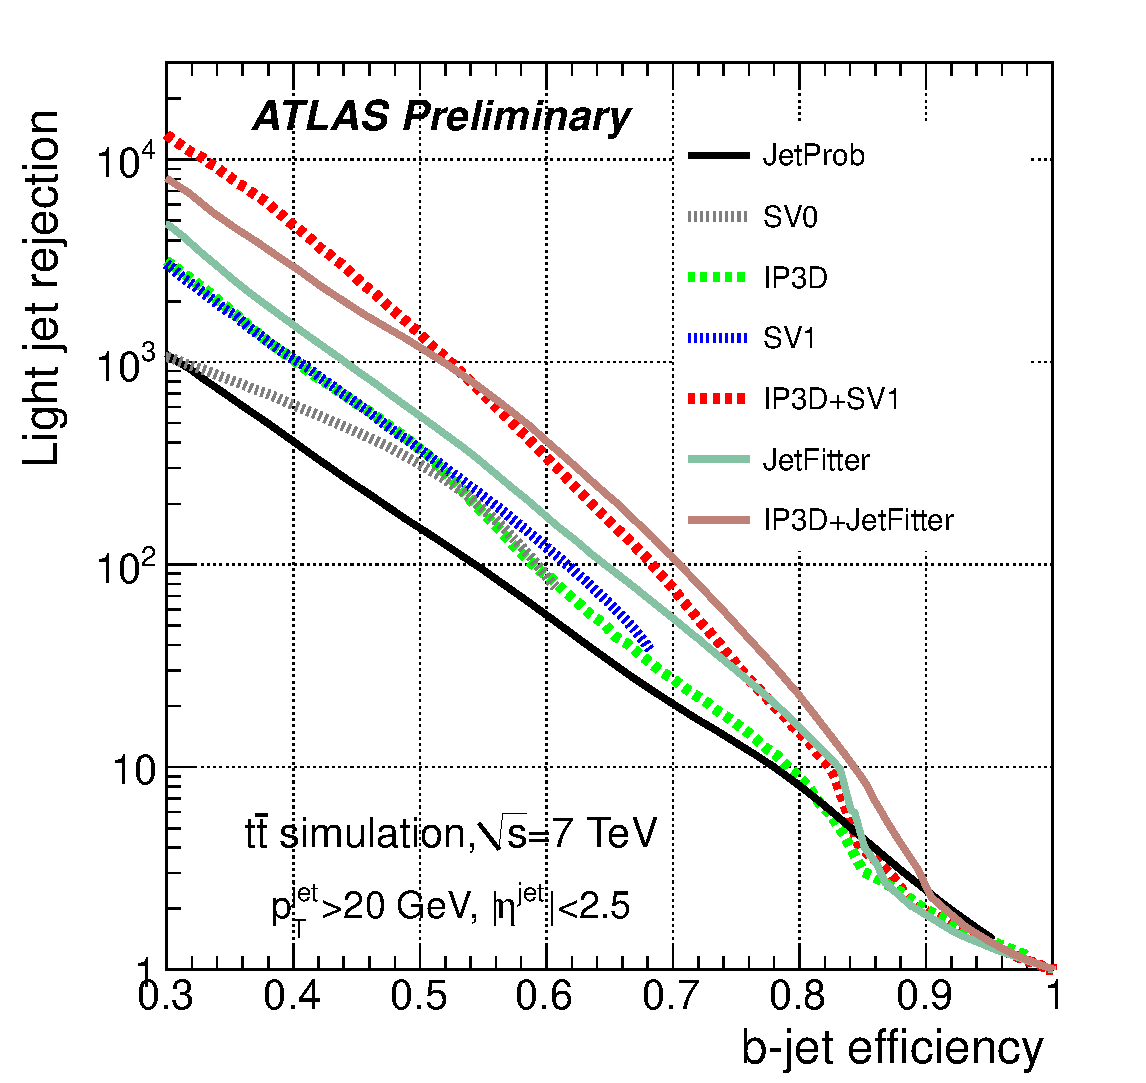
\includegraphics[width=0.6\textwidth]{figure/obj/btag_perf.pdf}

    \end{center}
    \caption{Light-jet rejection as a function of the b-jet tagging efficiency for different tagging algorithms~\cite{btagPerf}.
	    Rejection here is defined as the inverse of mistagging rate, and the distributions are referred to a 
		$\ttbar$ sample.}
   \label{fig:beff}
\end{figure}

The perfomance of the mentioned algorithms are evaluated in data  and compared to simulation in~\cite{btagPerf}.
B-hadron tagging efficiency and mistagging rate are the most common feature that describes the performance of a
b-tagging algorithm, Figure~\ref{fig:beff} shows the b-tagging efficiency as a fuction of the inverse of the mistagging rate
for different b-tagging algorithm, the tagging efficiency $\epsilon_b^{\ttbar}$ is usually referred to b-hadron in $\ttbar$ events
and totally specify a b-tagging selection point.
Correction due to non perfect modeling of b-tagging performance are evaluated by means of several methods
for 2012 data in~\cite{BtaggingScaleFactors, BtaggingScaleFactorsNew} and used as event weights in MC simulation.



\section{Electrons Reconstruction} \label{sec:elec}
Electron are reconstructed combining calorimeter and Inner Detector information,
an electron dedicated reconstruction algorithm is presented in~\cite{electronAlgo} is based on clusters reconstructed in the electromagnetic
calorimeter, which then are associated to tracks of charged particles reconstructed in the Inner Detector.


This analysis uses electrons found by the standard electron
identification algorithms ~\cite{AtlasCSCBook} that pass the {\tt Medium++}
criteria. A preselection is applied to the electrons to ensure that
the electron cluster has a transverse energy of $E_T > 15\GeV$, is
within the pseudorapidity range $|\eta|<2.47$, but is outside of the region
$1.37<|\eta|<1.52$. The first requirement ensures that the selected
electrons are within a range of $E_T$ where the electron reconstruction
and trigger efficiencies are well understood. The further requirements
ensure that the electron is reconstructed within the acceptance of
the ATLAS tracking, but outside of the transition region between the
barrel and end-cap calorimeters. 
In addition, the author is required to be either one or three, to ensure that the electron was 
reconstructed with either the standard electron algorithm or both the
standard and soft electron algorithms, respectively.
Finally, to ensure that the electron is not reconstructed within a region of the
calorimeter with readout problems, dead or non-nominal high voltage
conditions or suffering from high noise, the electron is rejected if
the cluster $\eta$ and $\phi$ position match a flagged region in the
Object Quality maps (OQ maps) provided by the egamma
performance group~\cite{EGammaRecomendations}.

For the electrons used in this analysis, the four-vector of the
particle is defined using the energy of the electron calorimeter
cluster and the direction of the electron track. Selections that
involve the electron position in the calorimeter, in this analysis the
$\eta$ and the OQ map selections, are however made using a four-vector built
entirely from the electron cluster properties. Both the energy scale
and resolution of the electrons used in this analysis are corrected,
following the recommendations of the EGamma performance group, by
using the {\tt egammaAnalysiUtils}
package\cite{EGammaRecomendations}. Energy scale corrections are
applied to electrons in data, whereas an additional smearing is
applied to the electron energy in MC.

In addition to the preselection defined above, isolation criteria are
defined to select electrons with little or no activity around
them. The calorimetric isolation, \etcone, is calculated as the sum of
the transverse energy of the additional topological clusters in the
electromagnetic and hadronic calorimeters in a cone of $\Delta R <
0.2$ around an electron\footnote{The $\Delta R$ variable is defined by
$\Delta R=\sqrt{(\Delta\eta)^2+(\Delta\phi)^2}$, where $\Delta \eta$
and $\Delta \phi$ correspond to the difference between
the pseudorapidities and azimuthal angles of the objects considered, respectively.}. 
The summed transverse energy is corrected, as a function of the
number of primary vertices in the event, to reduce the dependence on
pileup. In addition, the track isolation, \ptcone, is defined as the
scalar sum of the $\pt$ of all additional tracks with $\pt>1\GeV$ in a
cone of radius $\Delta R<0.4$ around an electron. In this analysis, an
electron with $\etcone/\pt<0.08$ and $\ptcone/\pt<0.06$ is considered isolated.


\subsection{Muons}
\label{sec:presel:muon}

Muons reconstructed by the STACO algorithm \cite{AtlasCSCBook} are
used in this analysis - those passing the STACO Loose quality criteria
are considered at the preselection stage, whereas the more stringent
STACO Combined quality criteria are required for the final muon
selection. Muons with a transverse momentum $\pt > 10\GeV$ and
within the pseudorapidity range $|\eta| < 2.5$ are selected. The
difference between the $z$ position of the muon track extrapolated to
the beam line and the primary vertex $z$ position must be less than 10
mm. 

Further quality criteria, as recomended by the Muon Combined Performance Group,
 are placed on the Inner Detector track of
the muon candidate to ensure that it is well reconstructed and to
reduce the fake rate due to decays of hadrons in flight. These
requirements ensure that multiple hits are found on the track in the
various layers of the ID, but take into account that dead or
uninstrumented regions may be crossed by the muon. Firstly, if the
muon passes through a section of the b layer of the Pixel detector
that is instrumented and not suffering from detector problems, there
should be one or more b layer hits on the track. The sum of the number
of hits on the track in the Pixel detector and the number of crossed
dead Pixel detector layers should be at least one. The sum of the
number of hits within the SCT detector and the number of dead SCT
modules crossed should be five or greater. The total number of crossed
dead Pixel detector and SCT detector layers should be less than three.
When within the angular region $|\eta|<1.9$, the sum of the TRT hits
and outliers on the track must be greater than five and the ratio of
TRT outlier hits to the total number of TRT hits must be less than
0.9. When the muon track is in the region $|\eta|\ge1.9$, the ratio of
TRT outlier hits to the total number of TRT hits must be less than 0.9
only if the sum of the TRT hits and outliers on the track is be
greater than five.

The momentum scale and resolution of the muons in this analysis are
corrected in MC following the recommendations of the Muon Combined
Performance group. The momentum corrections were measured by comparing
the di-muon mass peak position and resolution between data and MC at
the Z resonance. Smearings are applied in a coherent manner to
the ID, MS extrapolated and combined momenta of the transverse
momentum of the muon. In addition, a scale correction is applied to
the combined momentum momentum.

As for the electrons used in this analysis, both calorimeteric and
track based isolation are used to require little or no activity around a muon
in addition to the preselection above. The muon \etcone and \ptcone
variables are defined as for the electron case and are calculated
in cones of $\Delta R<0.2$ and $\Delta R<0.4$ around the muon, respectively. 
Once more \etcone is corrected as a function of the number of primary vertices in the
event, to reduce the dependence on pileup. In this analysis, a muon with
$\etcone/\pt<0.04$ and $\ptcone/\pt<0.06$ is considered isolated.



\subsection{b-Tagging}
\label{sec:presel:btag}

The tagging of jets due to the hadronisation of b-quarks is performed
using the MV1 b-tagging algorithm \cite{mv1}. This neural network based
algorithm uses the output weights of the JetFitter+IP3D, IP3D and
SV1 b-taggers as inputs. The working point that gives a nominal
b-tagging efficiency of 70\% on \ttbar samples is used.

\subsection{Taus}
\label{sec:presel:tau}

Hadronically decaying tau candidates are reconstructed using clusters
in both the electromagnetic and hadronic calorimeters. A preselection
is applied to the candidates that requires the reconstructed $\tau$
candidates to have a transverse momentum of $\pt>20 \GeV$ and to have
a reconstructed pseudorapidity of $|\eta| < 2.5$. Furthermore, it is
required that the candidates have either one or three tracks within a
cone of $\Delta R < 0.2$ associated to them and have a charge of $\pm
1$. Finally, the preselected tau candidates should pass the BDT-Medium
multivariant tau identification selection as well as the dedicated
electron and muon vetoes for hadronically decaying tau candidates.


\subsection{Overlap Removal}
\label{sec:presel:olr}

After the preselection of the physics objects needed for this
analysis, an overlap removal between the different objects is then
applied to avoid double-counting.  The distance between two objects in
rapidity $\Delta\eta$ and polar angle $\Delta\phi$ is defined as
$\Delta R=\sqrt{(\Delta\eta)^2+(\Delta\phi)^2}$. Overlap removal is
then applied in the following order:

\begin{itemize}
\item preselected electrons are removed if they overlap with a preselected muon  within $\Delta R < 0.2$,
\item preselected taus are removed if they overlap with a preselected muon or electron within $\Delta R < 0.2$,
\item preselected jets are removed  if they overlap with a preselected
  muon, electron or tau within \linebreak $\Delta R<0.2$.
\end{itemize}

\subsection{Missing Transverse Energy}
\label{sec:presel:met}

The missing transverse energy, \met, is calculated using the
RefFinal method, which takes the energy
deposited in the calorimeter, the muons reconstructed in the muon
spectrometer and tracks reconstructed in the inner detector as inputs. 
For this, the energy deposits are calibrated based
upon the high-$pt$~ physics object they are associated to, with an order
of preference of electrons, photons, hadronically decaying taus, jets
and finally muons. Any unassociated energy deposits are combined into
the so-called ``soft-term''. To reduce the effect of pileup on the
\met calculation, corrections are applied to both the jets in an event
and to the soft-term. Firstly, any jet with a pseudorapidity of $|\eta|<2.4$
that enters the \met calculation is weighted by it's JVF. Similarly,
the soft-term is weighted by the soft-term-vertex-fraction (STVF) of
the event - the ratio given by
\begin{equation}
STVF = \frac{\sum_{track, PV}\pt}{\sum_{track}\pt}
\end{equation}
where $\sum_{track, PV}\pt$ is the sum of the transverse momentum of
all tracks in the event associated to the primary vertex, but unmatched to physics
objects, and $\sum_{track}\pt$ is the sum of
the transverse momentum of all tracks in the event unmatched to
physics objects. Any calibration applied
to the energy or direction of the physics objects in the final
analysis is also propagated to the \met.


\subsection{Vertices} 
\label{sec:presel:vertices}
In this analysis vertices are selected that have a minimum of three
associated tracks: this helps to ensure that the selected vertices
come from beam-beam interactions rather than, for instance, cosmic
muons.

\subsection{Event Cleaning}
\label{sec:presel:celaning}

In addition to the data quality requirements described in section
\ref{sec:samples:dq}, further selections are applied to veto events
where bad jets are identified as arising from detector effects
(coherent noise in the EM and Tile calorimeters or spikes in the HEC
calorimeter), cosmics or beam based background. To reject events, the
recommendations of the JetEtMiss performance group \cite{TWIKI_JETMET}
are followed: Events are rejected if at least one AntiKt4LCTopo jet
with $p_T>20\GeV$, that passes the overlap removal with electrons,
muons and taus described in section \ref{sec:presel:olr}, fails the {\tt
BadLooseMinus} selection or points towards the hot Tile Calorimeter
cells identified in data taking periods B1 and B2 \cite{hottile}.

\begin{table}
  \begin{center}
    \begin{tabular}{cc}
      \hline \hline
      Physics Object & Preselection \\
      \hline
      Electrons & $\pt>15 \GeV$ \\
      & $|\eta|<1.37$ or $1.52<|\eta|<2.47$ \\
      & {\tt Medium++} \\
      & Author = 1 or 3 \\
      & Pass Object Quality Flag \\
      \hline
      Muons & $\pt>10 \GeV$ \\	
      & $|\eta|<2.5$ \\
      & isLoose STACO muon \\
      & Inner Detector track quality requirements \\
      & Inner Detector track $|z_0^{PV}|<10\mathrm{mm}$ \\
      \hline
      Jets & $\pt>30\GeV$ \\
      & $|\eta|<4.5$ \\
      & $|JVF|>0.5$ for jets with $|\eta|<2.4$ and $\pt<50\GeV$ \\
      \hline
      Jets (taggable) & $\pt>20\GeV$ \\
      & $|\eta|<2.5$ \\
      & $|JVF|>0.5$ for jets with $|\eta|<2.4$ and $\pt<50\GeV$ \\
      \hline
      Taus & $\pt>20 \GeV$ \\	
      & $|\eta| < 2.5$ \\
      & BDT Medium \\
      & $N_{tracks} =~ $1 or 3 \\
      & Author = 1 or 3 \\
      & Muon and Electron Veto \\
      \hline
      \met & RefFinal with STVF correction\\	
      \hline
      Vertices & $N_{tracks} \ge 3$ \\	
      \hline \hline
    \end{tabular}
    \caption{Summary of the preselections used for physics objects in this analysis}
    \label{tab:presel}
  \end{center}
\end{table}


\subsection{Monte Carlo Corrections}
\label{sec:presel:MCCorr}

The MC samples used on this analysis are corrected to account for differences
between the simulation and data in the trigger, lepton reconstruction and
identification and b-tagging efficiencies. Furthermore, the MC is
reweighted so that the vertex multiplicity distribution agrees with
that in the data.

\subsubsection{Trigger Efficiency corrections}
\label{sec:presel:TriggerCorr}

Correction factors are applied to the simulated trigger efficiency for
both the single electron, \linebreak \verb=EF_e24vhi_medium1=, and combined
electron-muon, \verb=EF_e12Tvh_medium1_mu8=, triggers used in this
analysis. The trigger efficiency for the \verb=EF_e24vhi_medium1= has
been measured with respect to offline electrons using a tag and probe
method in \Zee events \cite{TWIKI_EgammaWG_Eff_SF}. Scale factors are derived from the ratio of the
trigger efficiency measured in data and MC, measured as a
function of electron $\pt$ and $\eta$.

For the \verb=EF_e12Tvh_medium1_mu8= trigger, correction factors are
measured separately for the two individual legs of the trigger,
\verb=EF_e12Tvh_medium1= and \verb=EF_mu8= \cite{TriggerEfficiency}. The product of the two
correction factors is then used as the overall scaling factor. The
trigger efficiency for the \verb=EF_e12Tvh_medium1= leg has been
measured with respect to offline electrons using a tag and probe
method for \Zee events in both data and MC. Likewise, the
\verb=EF_mu8= trigger efficiency scale factors are derived using a tag
and probe measurement with \Zmumu events. Oncemore, scale factors are derived
from the ratio of the trigger efficiency measured in data and MC, measured as a
function of electron $\pt$  and $\eta$.

\subsubsection{Lepton Reconstruction Efficiency Corrections}
\label{sec:presel:LepEffCorr}

Further correction factors are applied to the MC samples to account
for differences in the lepton reconstruction and identification
efficiencies between data and simulation. Scale factors for the electron
identification and reconstruction efficiencies are measured separately
using a combination of $\Zee$ and $J/\psi \rightarrow ee$ tag and probe
measurements \cite{EGammaRecomendations}. 
Both sets of scale factors are measured as a function of the electron $E_T$ and $\eta$. 

Similarly, muon reconstruction efficiency scale factors
have been measured, using a \Zmumu tag and probe analysis, 
as a function of the muon $\pt$, $\eta$, $\phi$ and charge \cite{MuonReconstruction}.

\subsubsection{b-tagging Efficiency Corrections}
\label{sec:presel:BTagEffCorr}

Corrections are applied to the b-tagging efficiency and mistag rate in
MC, using a combination of the System8 and likelihood scale
factor measurements \cite{BtaggingScaleFactors}. Separate scale factors are applied, 
as a function of the jet \pt and $\eta$, 
based on the origin of the jet at truth level - ie. depending on if the jet originates from a $b$ quark, a $c$ quark, a $\tau$ lepton 
or a light quark.

\subsubsection{Pileup Reweighting}
\label{sec:presel:PileupCorr}

Differences between the distribution of the average number of
interactions per bunch crossing, $<\mu>$, in MC and data are
corrected by reweighting the MC $<\mu>$ distribution to that in the
full considered dataset. An additional scaling of $1.1 \times <\mu>$
is applied to the MC, which has been shown to improve the description
of the number of primary vertices distribution of the data.



%analysis
\newgeometry{left=3.7cm, right=3.7cm,bottom=4cm ,top=2cm}
\chapter[Neutral MSSM Higgs Bosons Search]{Search for neutral MSSM Higgs Bosons in  
$A/h/H \rightarrow \tau^{+}\tau^{-} \rightarrow e \mu + 4\nu$ decays} \label{chap:anal}


%
 \vspace{0.5cm}

%A search for neutral MSSM Higgs bosons with the ATLAS detector at the
%LHC is presented.  This analysis is based on an integrated luminosity of $20.3 ~fb^{-1}$
%of proton-proton collisions at a centre-of-mass energy of 8 TeV. 
%
%The analysis focusses on the decay of neutral Higgs bosons into a pair of tau
%leptons, which subsequently decay to an electron, a muon and four
%neutrinos. Furthermore, 
%
In the light of the recent discovery of a Higgs 
boson with mass of about 125~GeV at the LHC~\cite{AHiggsO,CHiggsO}, it remains an open question
whether this new particle is the only missing piece of the electroweak symmetry breaking
sector of the Standard Model or whether it is one of several Higgs bosons predicted in  theories 
that go beyond the SM. The most recent measurements \cite{ASpin0,ACouplings,CFermions,CWidth} of 
properties of the new boson show that they are fully compatible with the ones of the SM Higgs boson. 
Nevertheless, such a new particle can still be accommodated within theories beyond the 
standard model (BSM). Among  them, supersymmetric extensions of the Standard Model are theoretically favoured,
in particular the minimal supersymmetric extension (MSSM) which predicts five Higgs bosons, three of them electrically neutral.

In this chapter  the search  with the ATLAS detector for the neutral MSSM Higgs bosons decaying into pairs of tau leptons
in the fully leptonic final state is discussed. 
The result have been published in ref.~\cite{yuppy} as a part of the ATLAS search for the neutral
MSSM Higgs bosons in all final states of the tau lepton decays. 
The search is based on 20.3 $\text{fb}^{-1}$ of  data at a centre-of-mass energy of $\sqrt{s} = 8$~TeV
recorded by the ATLAS experiment during 2012.
This chapter is organised as follows: a brief summary of the MSSM Higgs sector 
and an introduction to the analysis strategy are given in Section~\ref{sec:intro},
while the event selection and categorisation are described in Section~\ref{sec:selection}. 
Section~\ref{sec:BackgroundEstimation} describes the estimation of the backgrounds and
in Section~\ref{sec:Systematics} methods for the evaluation of the  systematic uncertainties are discussed. Finally, 
in Section~\ref{sec:result} the result of the search are presented together with an overview of the statistical methods employed.


%There are two approach to explore the Higgs sector:
%one can study the coupling of the Higgs boson with vector
%bosons and fermions, those measure in fact are sensitive to new physics and can determine
%%given the unitarily property of scattering
%%amplitudes for longitudinal vectors and fermions, one can understand 
%if this particle is  fully responsible for
%the generation of all the SM particles masses. 
%Another approach is to directly search for %model dependent
%for additional Higgs es in a well defined model, which is the approach followed in this
%thesis where new neutral bosons are sought within the MSSM (see chapter \ref{}). 
%
%
%%Discovering the mechanism responsible for electroweak
%%symmetry-breaking and the origin of mass for elementary particles has been
%%one of the major goals of the physics program at the Large Hadron
%%Collider~(LHC)~\cite{LHC}.  In the Standard Model (SM) this mechanism
%%requires the existence of a single scalar particle, the Higgs
%%boson~\cite{ENGLERT,HIGGS,HIGGS2,HIGGS3,Guralnik:1964eu}.
%
%%This chapter is divided in three sections:
%%in section~\ref{sec:strategy} an introduction to experimental searches and to the strategy
%of this particular analysis is given, in section~\ref{sec:bkg} is described the core of this thesis
%work, i.e. the detail of the background modelling for this analysis, while in section~\ref{sec:result}
%the result of the search are presented.


\restoregeometry
\clearpage
\newpage

\section{Introduction } \label{sec:intro}

\subsection{The Higgs Sector in the MSSM}

\begin{figure}[tp]
     \begin{center}

            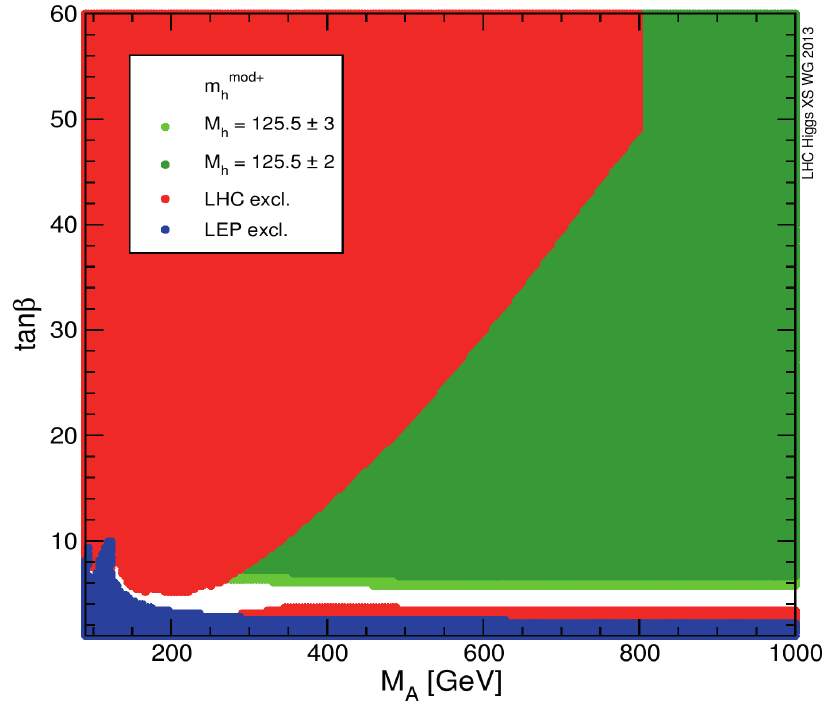
\includegraphics[width=0.7\textwidth]{figure/mh_mod.png}

    \end{center}
    \caption{Excluded and allowed regions of the MSSM  $m_{A} - \text{tan}\beta$ parameter space in the $m_{h}^{mod+}$ 
	benchmark scenario~\cite{LHCxsec}, based on direct Higgs boson searches at LEP 
	(blue) and LHC (red). The two green regions are compatible with the assumption that 
	the lightest MSSM Higgs boson, \emph{h}, has a mass of 125.5~GeV with an uncertainty of 2~GeV (dark green) 
	or 3~GeV (light green). }
   \label{fig:mhmod}
\end{figure}


In the minimal supersymmetric extension of the Standard Model
(MSSM)~\cite{MSSM1, MSSM2}, the Higgs sector is composed of two electroweak Higgs
doublets of opposite hyper-charge resulting in five observable Higgs
bosons, where two of them are neutral and $CP$-even
($h$,$H$), one is neutral and $CP$-odd ($A$) and two are charged
($H^\pm$).  At tree level, their properties such as masses, widths and
branching ratios are predicted depending on  only two parameters,
often chosen to be the mass of the $CP$-odd Higgs boson $m_A$ and
the ratio of the vacuum expectation values of the two Higgs doublets
$\tan\beta$ (for more details see chapter~\ref{chap:theory}).  
The MSSM predicts the existence of a Higgs boson with properties that  
resemble those of the SM Higgs boson in large regions of its parameter space. 
This is usually the case for the lightest Higgs boson, \emph{h}, while the other two, $H$ and $A$, 
tend to be degenerate in mass and decouple from gauge bosons.
%Production and decay mode 
%with vector bosons are forbidden for the CP-odd, $A$ and are suppressed for 
%the CP-even, $H$, Higgs bosons. 
On the other hand, the couplings of the latter two Higgs bosons to down (up) type fermions are enhanced
(suppressed) depending on the value of $\tan\beta$, such that for large $\tan\beta$
bottom-quarks and $\tau$ leptons  play an important role for Higgs bosons production and decay. 
 
The two dominant neutral MSSM Higgs boson production mechanisms 
at the LHC are gluon fusion, $gg\rightarrow A/H/h$, and 
the production in association with $b$-quarks, $pp \rightarrow b(b)A/h/H$, the latter becoming increasingly 
important for large values of $\tan\beta$. These  are the only production mechanisms
considered in this analysis. 
Assuming there are no decays into supersymmetric particles  (since they are too heavy)
and assuming that the lightest neutral CP-even Higgs boson $h$ is identified with the observed Higgs boson
of mass $\sim 125$~GeV, the dominant decay mode for the neutral MSSM CP-odd $A$ and CP-even $H$ Higgs bosons
 is the decay into a  $b$ and anti-$b$ quark pair, % $A/h/H \rightarrow b\bar{b}$, 
followed by the decay into $\tau$ leptons pairs. Since it is very difficult to distinguish the former decay 
from the large $b\bar{b}$ background, the decay mode 
$A/h/H \rightarrow \tau^+ \tau^-$  provides the highest sensitivity in the search for neutral MSSM Higgs bosons.

Searches for neutral MSSM Higgs bosons have been performed at
LEP~\cite{LEPLimits}, the
Tevatron~\cite{TevatronLimits1} and the LHC~\cite{CMSLimit, ATLASLimit}. 
In the following, the search for the neutral MSSM Higgs bosons  in the final state 
$A/h/H \rightarrow \tau^+ \tau^- \rightarrow e \mu +4\nu$ is presented. 
This search is complementary to the searches in other $\tau^+\tau^-$ final states
characterised by the presence of one or two hadronically decaying $\tau$ leptons. For low $m_A$ values
the $\tau^+ \tau^- \rightarrow e \mu +4\nu$ search channel provides a sensitivity to the signal comparable to the 
other final states, in spite of the fact that the $\tau\tau$ branching ratio to $e \mu +4\nu$ is only 6\%. 
This is mainly due to the high transverse momentum threshold at the trigger level for  hadronically decaying $\tau$ leptons,
which is necessary to keep the jet contamination rate at an acceptable level.

As it is virtually impossible to explore the full parameter space of the MSSM, 
which has a large number of free parameters, several benchmark scenarios have been  
introduced  fixing all parameters except $m_A$ and $\tan\beta$  to typical values for the most interesting 
physics cases.
With the recent Higgs boson discovery, benchmark scenarios of the MSSM have been updated to 
accommodate the  new experimental constraints. 
As an example, Figure~\ref{fig:mhmod} shows the currently excluded and allowed regions of the MSSM $m_{A} - \text{tan}\beta$ 
parameter space for the updated  $m_{h}^{mod+}$ benchmark scenario (see Section~\ref{sec:benchmark}). 
In this scenario, a large region of the $m_{A} - \text{tan}\beta$
parameter space is compatible with the assumption that the observed Higgs boson is in fact the 
neutral CP-even  Higgs boson $h$. A relatively large part of this parameter space is still experimentally unexplored,
which is a strong motivation to pursue the search for additional neutral MSSM Higgs bosons.


\subsection{Signal and Background Processes}

\begin{figure}[tp]
     \begin{center}
     \subfigure[]{		
            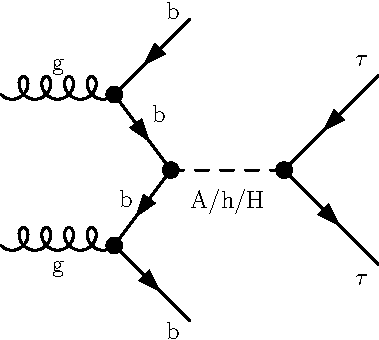
\includegraphics[height=3.4cm]{feyn_diagrams/diagrams/bbA.pdf}
     }\hspace{0.2cm}	
     \subfigure[]{		
            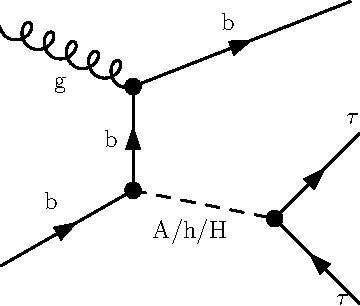
\includegraphics[height=3.4cm]{feyn_diagrams/diagrams/bbA2.pdf}
     }	\hspace{0.2cm}\\	
     \subfigure[]{		
            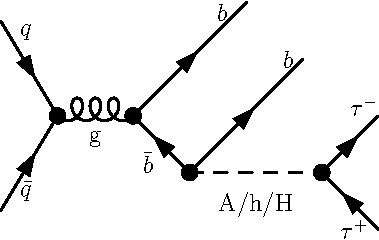
\includegraphics[height=2.9cm]{feyn_diagrams/diagrams/bbA3.pdf}
     }
     \subfigure[]{	
            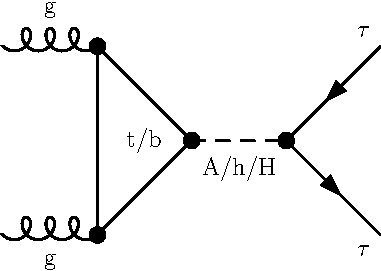
\includegraphics[height=2.9cm]{feyn_diagrams/diagrams/ggH.pdf}
	}	
     \end{center}
    \caption{Feynman diagrams for the production of the neutral MSSM Higgs bosons in association with  $b$-quarks (a,b,c) and via gluon fusion (d) 
	with subsequent decay into tau lepton pairs.}
   \label{fig:feyndiagSignal}
\end{figure}

Signal events in which the neutral MSSM Higgs bosons decay through 
$A/h/H \rightarrow \tau^+ \tau^- \rightarrow e \mu +4\nu$  are characterised 
by the presence of one electron and one muon of opposite charge. These two leptons are isolated and have 
relatively high transverse momenta. In addition, four neutrinos generate high missing transverse energy in the event. 
Figure~\ref{fig:feyndiagSignal} shows leading order Feynman diagrams for the two signal production modes considered,
gluon fusion and  associated production  with $b$-quarks.
The presence (absence) of a b-jet in the final state serves as  main characteristic for the categorisation
in the latter (former) events as described below.


The described signal topology  is common to several other  SM background  processes which in general  
have higher cross sections than the sought signal.
The dominant background processes are  $Z/\gamma^* \rightarrow \tau^+ \tau^- $ production
either via the  Drell-Yan process or in association with jets and  top quark production ($t\bar{t}$ and single top quark production ). 
Additional significant background contributions arise from  dibosons production 
($WW$, $WZ$, $ZZ$) and QCD multi-jet events with non-prompt leptons  from hadron decays.
Vector boson production ($\Wlnu$ or $\Zll$, where $\ell \equiv e,\mu$)  in association with jets 
is also considered, but has small impact on the total background contamination. Examples of 
leading order Feynman diagrams for the dominant background processes are shown in Figure~\ref{fig:feyndiagBack}.
The production cross sections times the branching fractions for signal and background processes are summarised in
Table~\ref{tab:MCxsec}. 
%The $W/Z$ and $b\bar{b}A/H/h$ production cross sections 
%are calculated to NNLO. The one for $\ttbar$, single top and dibosons cross sections are calculated at NLO.
%Finally, the direct $gg\rightarrow A/H/h$ signal cross sections 
%are calculated at NNLO and NLO for the top loop and the bottom loop respectively.
%

\begin{figure}[tp]
     \begin{center}
     \subfigure[]{		
            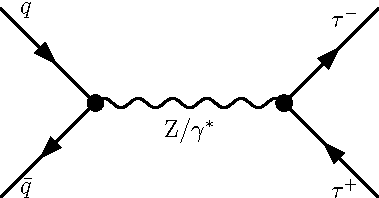
\includegraphics[height=3cm]{feyn_diagrams/diagrams/Ztautau.pdf}
     }\hspace{0.2cm}	
     \subfigure[]{		
            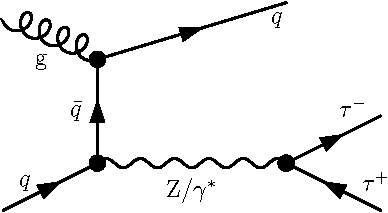
\includegraphics[height=3cm]{feyn_diagrams/diagrams/Z_plus_jet.pdf}
     }	
     \subfigure[]{		
            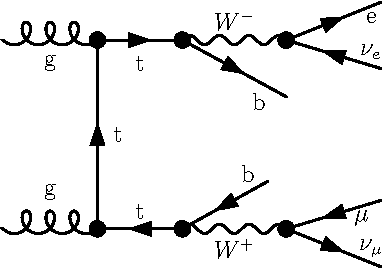
\includegraphics[height=3.5cm]{feyn_diagrams/diagrams/top.pdf}
     }\hspace{0.2cm}	
     \subfigure[]{	
            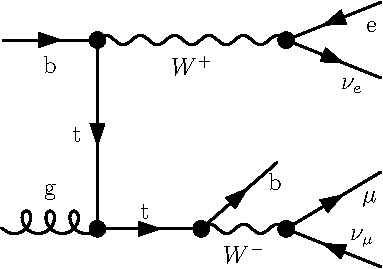
\includegraphics[height=3.5cm]{feyn_diagrams/diagrams/singletop.pdf}
	}	
     \subfigure[]{	
            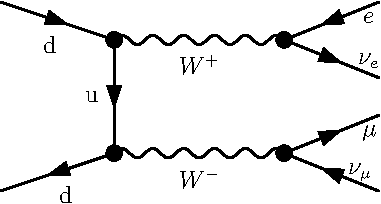
\includegraphics[height=3.2cm]{feyn_diagrams/diagrams/diboson.pdf}
	}\hspace{0.2cm}		
     \subfigure[]{	
            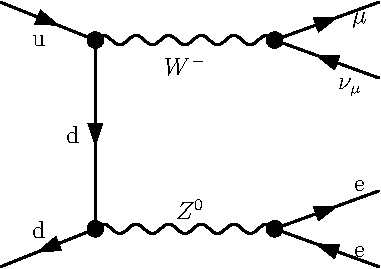
\includegraphics[height=3.2cm]{feyn_diagrams/diagrams/diboson2.pdf}
	}	
     \end{center}
    \caption{Examples of tree level Feynman diagrams for  the most important background processes. The production of 
	 $Z/\gamma^* \rightarrow \tau^+ \tau^- $, either via the Drell-Yan process or in association with jets,  is shown in (a) and (b)
	respectively, top quark pair and single top quark production in (c) and (d), while $WW$ and $WZ$ production in (e) and (f).
	}
   \label{fig:feyndiagBack}
\end{figure}


%The values of the steering parameters used for the HERWIG, JIMMY and PYTHIA
%generators are described in Ref.~\cite{ATLASMC09Tune}.

\begin{table}[!tp]
\begin{center}
\caption{The cross sections times by the relevant branching ratios~(BR) for signal and the considered
background processes, with $\ell= (e, \mu, \tau)$. 
Signal cross sections are calculated for the $m_{h}^{mod}$ scenario assuming
 $m_A=150$~GeV and $\tan\beta=20$. The masses of the other two neutral MSSM Higgs bosons are 
	in this case  $m_H=151$~GeV and $m_h=125$~GeV.} 
\vspace{2mm}
%\begin{footnotesize}
\begin{small}
\begin{tabular}{lr}
\hline \hline
Process                                                                 & Cross-section~$\times$ BR (pb) \\ [1pt]
\hline
\multicolumn{2}{c}{Signal ($m_A=150$~GeV, $\tan\beta=20$, $m_{h}^{mod}$ scenario) }  \\ [1pt]

$gg\rightarrow A/h/H \rightarrow\tau\tau \rightarrow e\mu+ 4\nu$                 &  $0.24 /0.20 / 0.95 $ \\
$pp \rightarrow b\bar{b}A/h/H \rightarrow \tau\tau \rightarrow e\mu + 4\nu$       & $0.53 /0.05 / 0.49   $ \\[1pt]
\hline
\multicolumn{2}{c}{Backgrounds} \\[1pt]
$W\rightarrow \ell \nu$+jets                           & 12.22$\times 10^3$ \\
$Z/\gamma^{*}\rightarrow \ell\ell$+jets       & 5.5$\times 10^3$ \\
$t\bar{t} \rightarrow \ell \ell + X$                                                              & 137.3 \\
Single top quark ($t-$, $s-$ and $Wt-$channels) $\rightarrow \ell + X$               & 28.4, 1.8, 22.4 \\
Dibosons (WW, WZ and ZZ ) $\rightarrow \ell \ell+ X$                                          & 20.6, 6.8, 1.55 \\ [1pt]
\hline 
\hline
\end{tabular}
\end{small}
 \label{tab:MCxsec}

\end{center}
\end{table}


\subsection{Analysis Strategy} \label{sec:strategy}


In this thesis, a search for the neutral MSSM Higgs boson decays
$A/h/H \rightarrow \tau^+ \tau^- \rightarrow e \mu +4\nu$ is presented. The $ee +4\nu$ and $\mu\mu +4\nu$ final states 
are not considered since  large background contributions are expected  from $\Zee$ and $\Zmumu$ decays,  respectively, 
such that the sensitivity of the search in these final
state is significantly reduced.

Candidate events are selected based on the topological properties of Higgs boson production
and decay. The  presence of exactly one electron and one muon is required in each event. The electron and the muon are required to be 
 isolated and of opposite electrical charge.
The  events are categorised into two orthogonal categories. In the so called  \emph{b-vetoed} event category,
the absence of b-tagged jets is required, 
thus searching mainly for the signal production via gluon fusion. The main background 
process in  this category is $\Ztautau$. 
In contrast, the presence of exactly one  b-tagged jet is required in the so called \emph{b-tagged} event category, 
in which predominantly the signal production in association with b-quark is searched for. The requirement of a b-jet 
in the final state suppresses the $\Ztautau$ background, consequently, $\ttbar$ and single top quark  production
are the main background processes in this event category. Further selection criteria are introduced in both event categories
optimised to enhance the signal with respect to the background.

The  search is performed within the MSSM $m_h^{mod}$ benchmark scenario
scanning the $m_A - \tan\beta$ plane in the range $90 \leq m_A \leq 300$ GeV and $5 < \tan\beta < 60$.
The signal event yields and kinematical distributions are predicted by simulation.
The contribution of the dominant $\Ztautau$ background process is measured in a dedicated  signal-depleted control data sample
in order to reduce the systematic uncertainties of the simulation. Similarly, the QCD multi-jet background contribution 
is also estimated from a dedicated data control sample since this background process is hard to model. The
%the large cross section puts high demands on the number of simulated events.
contributions of  all  other background processes  are estimated by simulation.
The modelling of the background processes is  validated using different signal-depleted validation data samples where
good agreement is found.

Systematic uncertainties  on cross section calculations and the modelling of the detector response for 
simulated signal and background processes are taken into account. For background processes  determined from  data,
the uncertainties of the measurement methods are evaluated.

The statistical interpretation of the data is based on the 
comparison of the observed $\tau\tau$ invariant mass distributions with the predictions of the  background-only and signal-plus-background
hypotheses. Exclusion limits on the signal production are set by means of a binned profiled likelihood ratio
test statistic within the MSSM $m_{h}^{mod}$ scenario as constraints in the 
 $m_A - \tan\beta$ plane. Furthermore, the data are interpreted in a less model-dependent
way in terms of  upper limits on the cross section for the production of a generic Higgs boson $\phi$ with   mass  $m_\phi$ 
via the  processes $pp \rightarrow b\bar{b}\phi$ and $gg \rightarrow \phi$.


 

%neutral MSSM Higgs bosons with the ATLAS experiment at CERN is
%presented, using proton-proton collisions at centre-of-mass energy of
%8~TeV, with a recorded integrated luminosity of
%$20.3 \ifb$.



\subsection{Data and Simulated Event Samples}
\label{sec:sample}
\subsubsection{Data Sample}

The  presented results  are based on proton-proton collision data
recorded by the ATLAS experiment during 2012 at a centre-of-mass energy of $\sqrt{s}=8$~TeV
corresponding to an integrated luminosity of 20.3 fb$^{-1}$.
The events used in this analysis are recorded using a combination of a
single electron trigger  and combined electron-muon triggers. Only events 
recorded with  all  relevant components of the ATLAS detector 
fully operational are considered.
Additional data quality requirements are applied according to~\cite{ATLASCLEANING} rejecting 
events %with data corruption due to the LAr and Tile calorimeters and
with jet activity in known noisy calorimeter regions. 




\subsubsection{Signal Samples}
%Both the signal and background process modelled by Monte Carlo (MC)
%simulation were produced within the ATLAS MC12a production campaign.
%The generators used for the different processes are described below.
Signal production via the gluon fusion process $gg\rightarrow A/H/h$
was simulated with POWHEG~\cite{POWHEG} and the associated
$b\bar{b}A/H/h$ production with SHERPA~\cite{SHERPA}.  The
pseudo-scalar Higgs boson samples were generated in the mass range from
90~GeV to 300~GeV assuming $\tan\beta = 20$. Re-weighting of the production cross sections is applied 
to simulate other $\tan\beta$ values. All three  neutral Higgs bosons $A,h,H$ are assumed to decay 
with the same kinematical properties. The $m_h^{\mathrm{mod}}$ MSSM benchmark scenario is assumed
for the prediction of the mass and cross sections of the three neutral Higgs bosons for  given $m_A$ and $\tan\beta$ values.


\subsubsection{Background Samples}
The production of $W$ and $Z/\gamma^*$ bosons in association with jets
was simulated with the ALPGEN~\cite{Alpgen} generator. 
%This employs
%the MLM matching scheme~\cite{MLM} between the hard process,
%calculated with leading-order matrix elements for up to five jets, and
%the parton shower.  
The $t\bar{t}$ process was generated using the POWHEG program. Single top quark 
production via the  s-channel and via the   $Wt$ process was
 generated using MC@NLO~\cite{MCatNLO}, while single top quark production via 
t-channel  was generated with the AcerMC~\cite{AcerMC}.  Diboson processes ($WW$, $WZ$, $ZZ$) were generated with
 HERWIG~\cite{Herwig}.  For all ALPGEN  
and MC@NLO event samples described
above, the parton shower and hadronization were simulated with the  HERWIG
and the underlying event activity with the JIMMY~\cite{JIMMY} programme.
%The loop-induced $gg\rightarrow WW$ processes were generated using gg2WW~\cite{GG2WW}.  We are not using it Xsec very small
Different sets of parton density functions (PDFs)  are used depending on
the generator: CTEQ6L1~\cite{CTEQ6} is used with the ALPGEN and AcerMC while
CT10~\cite{CT10} is used with SHERPA, POWHEG and MC@NLO. 

TAUOLA~\cite{TAUOLA} and PHOTOS~\cite{PHOTOS} are used to model the
tau lepton decay and additional photon radiation from final state charged leptons
in the leading-log approximation, respectively.

The ATLAS detector response is simulated for all generated samples using the GEANT4~\cite{Geant4,ATLASSIM} package.
The reconstruction of physics objects, described in chapter~\ref{chap:obj}, is performed with the same software as used for 
the data.
The effects of simultaneous recording of additional proton collisions from the
same or neighbouring bunch crossings (pile-up) are taken into account in the detector
simulation. 



\section{Event Selection and Categorisation}\label{sec:selection}


\subsection{The Common Selection Criteria}\label{sec:presel}

According to the kinematical properties of signal events, each event in data and simulation have to satisfy
the selection criteria described in the following. Since these are shared by both the b-tagged and the b-vetoed event category,
they are referred to as common selection criteria:


\begin{enumerate}[label=(\roman*)]
\item The trigger selection requires the presence of a single electron with $\pt > 24$~GeV or, alternatively,
	an electron with  $\pt > 12$~GeV togheter with a muon with  $\pt > 8$~GeV. 

\item At least one reconstructed vertex with more that three associated tracks in order to 
	reject background from cosmic muons.

\item Exactly one reconstructed ``Tight'' electron with $|\eta| < 1.37 $ or $1.52 < |\eta| < 2.47$ and
	 $\pt > $ 15 or 25~GeV, depending on the trigger that selected the event. 

\item Exactly one ``Combined'' muon with $|\eta| < 2.5$ and  $\pt > $ 10~GeV.

\item The electron have to be isolated with $E_T^{cone}/ \pt < 0.08$ and $P_T^{cone}/ \pt < 0.06\,.$ 

\item The muon have to be isolated with  $E_T^{cone}/ \pt < 0.04$ and $P_T^{cone}/ \pt <  0.06\,.$ 

\item Muon and electron have to be of opposite charge.

\item Removal of overlap between reconstructed electron, muon, $\tau$-jets and jets is performed.

\item The event is rejected if at least one hadronic $\tau$ lepton decay is found with  $\tau$-jet transverse 
	momentum  $\pt > $ 15 GeV. $\tau$-jets candidate are required to be associated to one or three charged tracks,
	for the identification a ``Medium'' BDT working point is chosen, additionally, a BDT-based electron veto is 
	applied. 

\item To reduce QCD multi-jet background contamination, the invariant mass of electron and muon has to be 
	greater than 30 GeV.

\end{enumerate}
Details on  the definition of physics objects and the applied quality criteria  can be found in  chapter~\ref{chap:obj}.

Events accepted by the common selection criteria are divided into \emph{b-tagged} and \emph{b-vetoed}  categories by requiring the presence 
or the absence, respectively, of exactly one b-tagged jet  in the event. A jet is tagged  as a b-jet if  it has 
$\pt > 20$ GeV, $|\eta| < 2.5$, $\text{JVF} > 0.5$ and if it passes  the $MV1$ b-tagging criteria corresponding to 
70\% of b-quark efficiency $\epsilon_b^{\ttbar}$ in $\ttbar$ events. Further selection criteria
are applied to each category and optimized separately as described in the following.

\subsection{b-Vetoed Event Category}\label{sec:veto}
%\subsection{Selections}

%The final state of Higgs decaying into tau pair coincide with the one from  
A veto on the presence of b-tagged jets in the final state allows for the selection of signal events
produced predominantly via gluon fusion. In this event category, the 
$\Ztautau$  process is an irreducible background due to the same topology of the Higgs and $Z$ boson decay.
Other background processes can  be discriminated from the signal due to their kinematical properties.
The $\tau$ leptons from the Higgs boson decay are highly boosted and so are their decay products, resulting
in significantly different lepton kinematics in the Higgs decays with respect to  diboson or $\ttbar$ background processes. 
Firstly, the electron and muon from Higgs boson decay are predominantly 
emitted back-to-back as illustrated in Figure~\ref{dphi} which shows
the angular distance $\Delta\phi_{e,\mu} = |\phi_{e} - \phi_{\mu}|$  between the two leptons in the transverse plane 
for the signal and background processes. Secondly, the neutrinos from Higgs boson decay  are predominantly
collinear with the charged leptons. Thus, the angular correlation between the direction of the missing transverse energy 
and the two charged leptons in the transverse plane, 
%re can be mathematically seen as the sum of scalar product between missing energy and the leptons four-vectors in the
%transverse plane, if the vectors are normalised to unit versors then what remains is a relation only between angles:
$$ \hat{E}_{T}^{miss} \cdot ( \hat{P}_{T}^{\mu} + \hat{P}_{T}^{e} ) = cos(\Delta\phi_{E_{T},\mu}) 
+ cos(\Delta\phi_{E_{T},e}) = \sum_\ell cos(\Delta\phi_{E_{T},\ell}) \,,$$
tends to zero as shown in Figure~\ref{sumcosphi}. 
These two features are used to discriminate between  signal and the W boson, top quark and  dibosons background processes.
%ck-to-back and the neutrinos not collinear with them.
%In b-vetoed category these two variables are sufficient to suppress contribution from dibosons,
No further selection criteria are applied in the b-vetoed category, since  no significant improvement
in signal sensitivity could be achieved.
The described selection criteria are listed in Table~\ref{tab:sel}, while in Table~\ref{tab:eventsel:bveto}
the predicted numbers of signal and background events after each selection stage  are shown.


\begin{table}[!t]
  \begin{center}
   %\begin{footnotesize}	
    \caption{Summary of the event selection criteria in the b-tagged and b-vetoed event categories applied after the common 
	event selection has been performed.}
	\vspace{2mm}
    \begin{tabular}{p{4cm}c}
      \hline \hline
      Category & Selection \\ [3pt]
      \hline
%      Common Selection 	&  Trigger \\
%	&	At least one reconstructed vertex with $> 3 $ tracks \\
%	& 	Exactly one tight isolated electron with $\pt > 15 $ or 25 GeV  \\
%	&	Exactly one Combined isolated muon with  $\pt > 10$ GeV \\
%	& 	Opposite charge between electron and muon \\ 
%	&	Overlap removal\\
%	&	Tau Veto \\
%	&	$M_{e-\mu} > 30$ GeV \\
%      \hline
      b-vetoed &  No b-tagged jets \\	
      & $\Delta\phi_{e,\mu}>1.6$ \\
      & $\sum\cos\Delta\phi_{E_{T},\ell} > -0.4$ \\[5pt]
      \hline
      b-tagged & Exactly one b-tagged  jet \\
      & $\Delta\phi{e,\mu}>2$ \\
      & $\sum\cos\Delta\phi_{E_{T},\ell} > -0.2$ \\
      & $ H_T < 100$ GeV \\
      & $P_{T\mu} + P_{Te} + \met < 100$ GeV \\[3pt]
      \hline \hline
    \end{tabular}
    \label{tab:sel}
  %\end{footnotesize}
  \end{center}
\end{table}

\begin{figure}[p]
     \begin{center}
     \subfigure[]{		
            \includegraphics[page=16,width=0.45\textwidth]{figure/final_plots/presel_total_final.pdf}
            %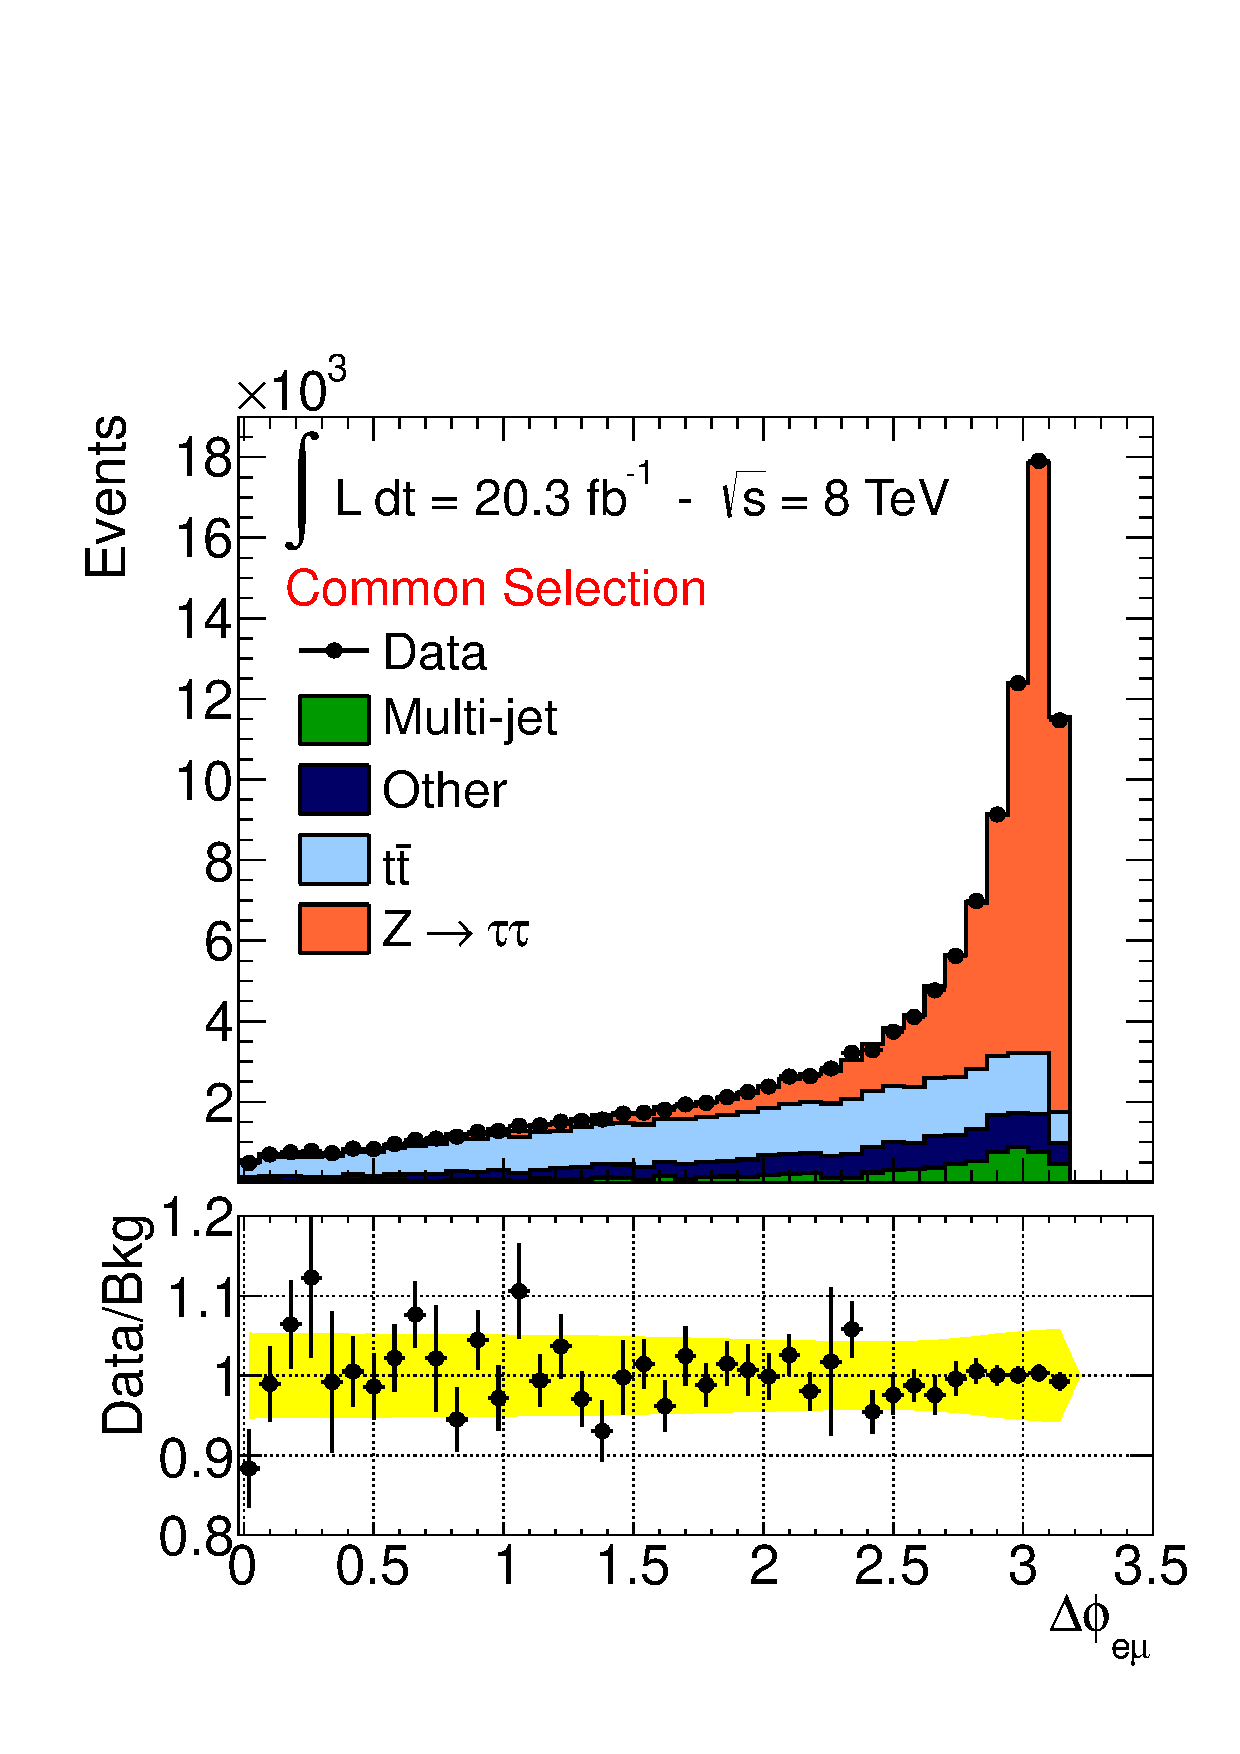
\includegraphics[width=0.47\textwidth]{figure/final_plots/std_presel_deltaPhi.pdf}
	    \label{dphi}	
    }	
     \subfigure[]{		
            \includegraphics[page=20,width=0.45\textwidth]{figure/final_plots/presel_total_final.pdf}
            %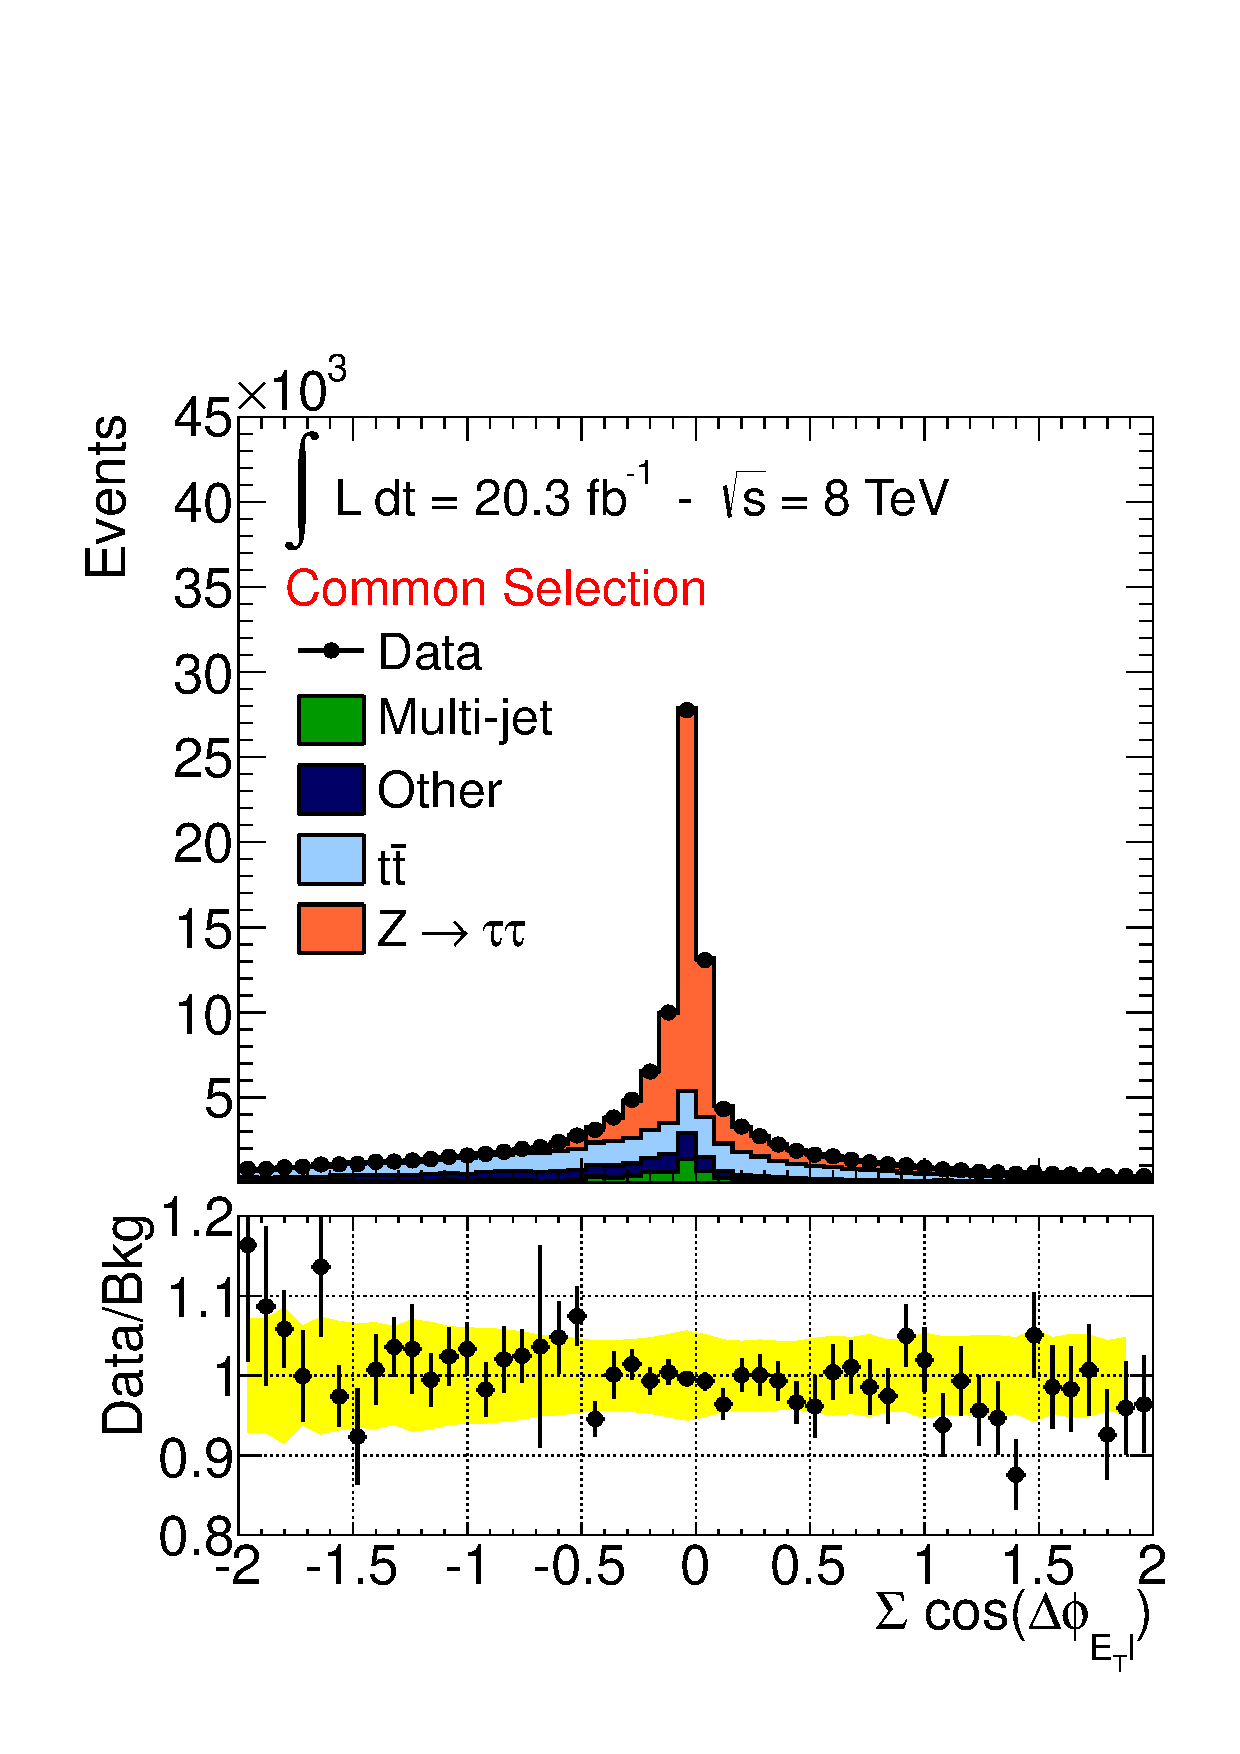
\includegraphics[width=0.47\textwidth]{figure/final_plots/std_presel_sum_cos_deltaPhi.pdf}
	    \label{sumcosphi}	
     }	
    \subfigure[]{		
            \includegraphics[page=19,width=0.45\textwidth]{figure/final_plots/presel_total_final.pdf}
            %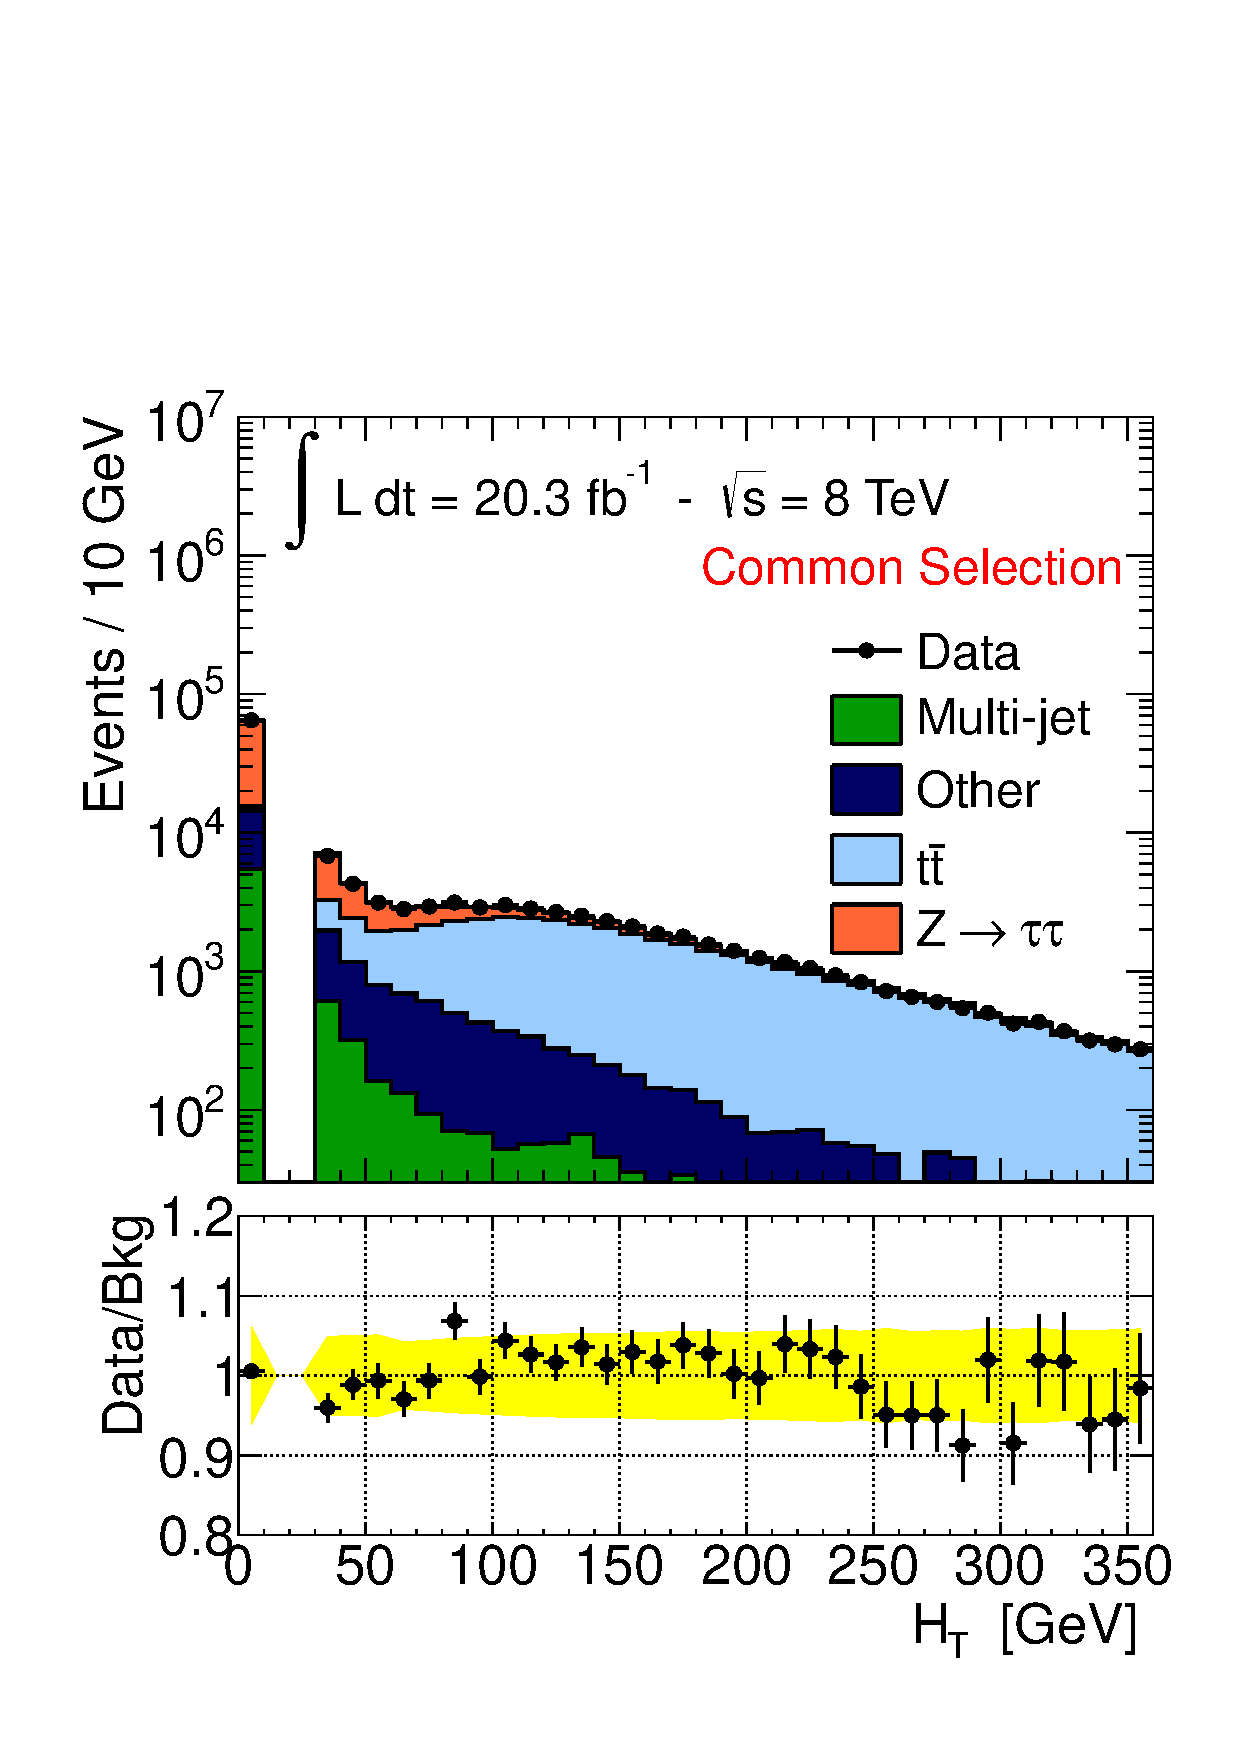
\includegraphics[width=0.47\textwidth]{figure/final_plots/std_presel_Ht.pdf}
	    \label{Ht}	
     }	
     \subfigure[]{		
            \includegraphics[page=12,width=0.45\textwidth]{figure/final_plots/presel_total_final.pdf}
            %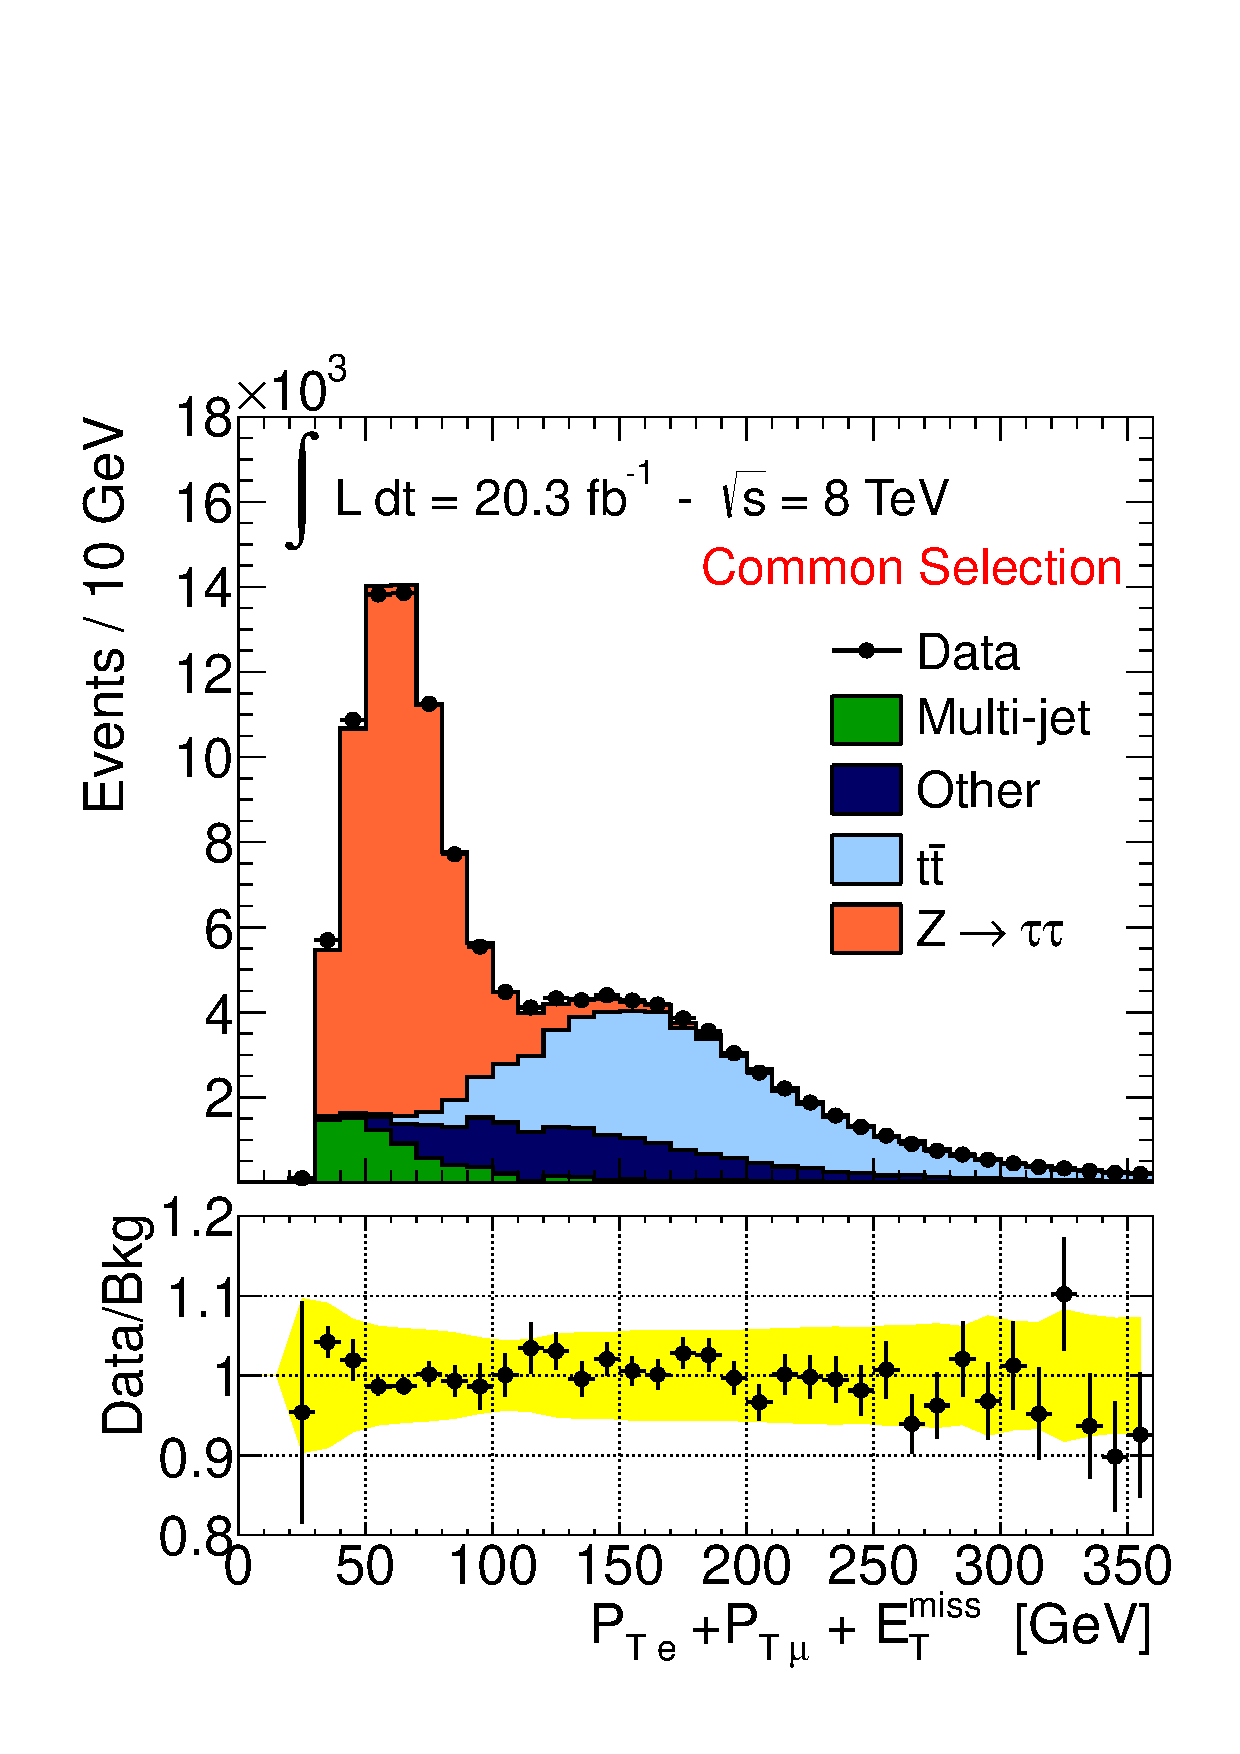
\includegraphics[width=0.47\textwidth]{figure/final_plots/std_presel_Et_plus_leptonPt.pdf}
	    \label{sumlepPt}	
     }	

    \end{center}
    %\caption{Distributions of discriminating variables electron-muon angular separation
%	$\Delta\phi{e,\mu}$ (a), the angular correlation between charged lepton and $\met$ $\sum\cos\Delta\phi_{E_{T},\ell}$ (b),
%	the total sum of jet $\pt$ (c), the sum of charge lepton $\pt$ and $\met$ (d), after the common selection has been applied.
% 	The notation ``Other'' stands 	for the electroweak processes $\Wlnu$, $\Zll$, Diboson and single top quark production.
%	The prediction for the background contributions is determined as described in 	Section~\ref{sec:BackgroundEstimation}.
%	The superimposed signal is obtained assuming the $m_h^{mod}$ scenario for $m_A=150$~GeV and $\tan\beta=20$ and it is scaled
%	by a factor ten. The error bars on the ratio of observed and predicted events represent the statistical uncertainty on data,
%	whereas the yellow and red band indicates the systematic and statistical uncertainty on the background prediction (see Section~\ref{sec:Systematics}),
%	respectively.}
    \caption{Distributions of discriminating variables (see text) after the common selection has been applied.
 	The notation ``Other'' stands 	for $\Wlnu$, $\Zll$, diboson and single top quark processes.
	The prediction for the background contributions is determined as described in 	Section~\ref{sec:BackgroundEstimation}.
	For the signal the $m_h^{mod}$ scenario is assumed with  $m_A=150$~GeV and $\tan\beta=20$ and it is scaled
	by a factor ten. The yellow and red band indicates the systematic and statistical uncertainty on the background prediction, respectively.}
   \label{fig:selections}
\end{figure}

\subsection{b-Tagged Event Category}\label{sec:tag}
The requirement of exactly one b-tagged jet in the b-tagged event category predominantly selects signal events 
where the Higgs bosons are produced in  association with b-quarks.
Background processes with b-jets, as the $\ttbar$ and single top quark production, are enhanced compared to the $\Ztautau$ background.
Also in this category requirements on $\Delta\phi_{e,\mu}$ and $\sum\cos\Delta\phi$  are imposed to reduce the top quark and diboson background contributions
as described for the b-vetoed event category. Further selection criteria specific for the b-tagged category
are employed  as described below.

\begin{table}[!t]
  \caption{Number of observed and predicted signal and background events, after each selection stage in the b-vetoed event category.}
	\vspace{1mm}
  \centering
   \begin{footnotesize}	
  \begin{tabular}{ccccc}
    \hline\hline
	&	Common Selections			&	n(b-jet)=0	&	$\Delta\phi(e-\mu)>1.6$	&	$\sum\cos\Delta\phi > -0.4$ 		\\	
    \hline
Multi-jet	&	6693	$\pm$	456	&	6357	$\pm$	461	&	5322	$\pm$	438	&	4180	$\pm$	230	\\
\Zll 		&	569	$\pm$	48	&	564	$\pm$	48	&	516	$\pm$	47	&	432	$\pm$	44		\\
\Wlnu		&	1625	$\pm$	155	&	1604	$\pm$	155	&	1145	$\pm$	125	&	660	$\pm$	100		\\
Dibosons	&	9338	$\pm$	48	&	9235	$\pm$	48	&	7358	$\pm$	43	&	2921	$\pm$	27		\\
\ttbar		&	40632	$\pm$	106	&	7707	$\pm$	46	&	5044	$\pm$	37	&	2228	$\pm$	25		\\
Single Top	&	4449	$\pm$	44	&	1664	$\pm$	27	&	1124	$\pm$	22	&	443	$\pm$	14	\\
\Ztautau	&	61503	$\pm$	68	&	60440	$\pm$	67	&	58078	$\pm$	65	&	54680	$\pm$	60	\\
    \hline
Total		&	124800 $\pm$ 	500	& 	87600 $\pm$ 400		&	78600 $\pm$	400	&	65540 $\pm$	260 \\
\hline
Data	&	125886			&	89155			&	79729			&	65917		\\
   \hline
   \hline
  \end{tabular}
  \label{tab:eventsel:bveto}
   \end{footnotesize}	
\end{table}

\begin{table}[tp]
  \caption{Numbers of observed and predicted signal and background events after each selection stage in the b-tagged event category.}
	\vspace{1mm}
  \centering
   \begin{footnotesize}	
  \begin{tabular}{cccccccc}
    \hline\hline
	& 	n(b-jet)=1			&	$\Delta\phi$&	$\sum\cos\Delta\phi$			&	$P_{T\mu} + P_{Te} + \met$&	$ H_T$	\\
   \hline
Multi-jet	330	$\pm$	40	&	208	$\pm$	27	&	135	$\pm$	22	&	114	$\pm$	17	&	101	$\pm$	15	\\
\Zll 	&	5.2	$\pm$	1.8	&	2.3	$\pm$	1.1	&	2.3	$\pm$	1.1	&	1.7	$\pm$	1.0	&	1.3	$\pm$	1.1		\\
\Wlnu	&	20	$\pm$	6	&	15	$\pm$	6	&	13	$\pm$	6	&	10	$\pm$	6	&	10	$\pm$	6		\\
Dibosons	&	99	$\pm$	5	&	63	$\pm$	4	&	36.4	$\pm$	3.0	&	14.8	$\pm$	1.8	&	14.4	$\pm$	1.9		\\
\ttbar	&	19810	$\pm$	70	&	9680	$\pm$	50	&	6450	$\pm$	50	&	808	$\pm$	15	&	330	$\pm$	10		\\
Single Top &	2456	$\pm$	33	&	1223	$\pm$	23	&	784	$\pm$	18	&	122	$\pm$	7	&	90	$\pm$	7		\\
\Ztautau &	952	$\pm$	9	&	625	$\pm$	7	&	540	$\pm$	7	&	482	$\pm$	6	&	418	$\pm$	6		\\
   \hline
Total 	&	23570  $\pm$ 90		&	11750  $\pm$ 60		&	7960  $\pm$ 60		&	1552  $\pm$ 25 		&     	963  $\pm$ 21 \\
   \hline
Data	&	23352			&	11490			&	7568			&	1528			&	904						\\
%Signal		&				&	-			&	-			&	-			&	-						\\
    \hline
    \hline
  \end{tabular}
  \label{tab:eventsel:btag}
   \end{footnotesize}	
\end{table}  

Signal events in this event category can be discriminated from  top quark given their relatively low jet activity. 
The $\ttbar$ events are likely to have two or more highly enegetic reconstructed jets, unlike the signal
b-jets which have relatively low energy. Low jet activity is ensured by requesting the sum of the jet transverse momenta $H_T$ to be small.
The $H_T$ distribution is shown in Figure~\ref{Ht}. The jets used for the calculation of $H_T$  have 
to fullfill $\pt > 30 $ GeV, $|\eta| < 4.5$  and $\text{JVF} > 0.5 $ (if $|\eta| < 2.5$).

Another feature that discriminates top quark  pair production from the Higgs boson signal is the higher invariant mass 
of the decay products of the former as the highest Higgs mass considered in this  search is 300 GeV.
The sum of the electron and muon transverse momenta and of  \met is  used as 
discriminating variable and is shown in Figure~\ref{sumlepPt}$\,.$

The optimized selection criteria for the b-tagged event category are shown in Table~\ref{tab:sel}.
In Table~\ref{tab:eventsel:btag} the predicted numbers of signal and background events after each selection stage are given in 
 the b-tagged event category.





\subsection{Mass Reconstruction with the MMC Technique}\label{sec:mmc}

Acurate invariant mass reconstruction of a di-$\tau$ resonance is a challenging task due to the undetected neutrinos. 
In this analysis there are a total of four neutrinos in the final state, two from  each 
of the $\tau$ lepton decays.
% In case of leptonic decay of the $\tau$ leptons
%a total of four neutrinos are involved in the final state. 
The invariant mass depends on eight unknown which are the components of the total neutrino four-momenta 
in each of the $\tau$ lepton decays. These unknowns are  constrained by the two measured component of the 
 missing transverse energy $\vec{E}_T^{miss}$ and by  the $\tau$ lepton mass $M_{\tau}$ via the following four equations:
% 
%In case of leptonic decay of both $\tau$ leptons a pair of neutrinos for each
%of them are involved in the final state,  the system presents then eight unknowns, which corresponds to the four-momentum of the neutrinos pairs.
%Four additional kinematic constraint are set by the following equations:
%There are four additional constraint 
%which come from the measurement of \MET and from the fact that each single decay should have invariant mass equal to the tau mass:
\begin{equation} \label{eq:MMC}
\begin{split}
%\begin{align}
%\begin{gather*}  
&\vec{E}_T^{miss} = \vec{P}_{T}^{mis_{1}} +  \vec{P}_{T}^{mis_2} \,,\\
&M_{\tau_{i}}^2 = m^2_{mis_{i}} + m^2_{vis_{i}} + 2 \mathbf{P}_{vis_i} \cdot \mathbf{P}_{mis_i} \,, \\
%\end{align}
%\end{gather*}
\end{split}
\end{equation}
where \emph{i}=1,2 distinguish the two $\tau$ leptons.
$\vec{P}_{T}^{mis_{i}}$, $m_{mis_{i}}$ and $\mathbf{P}_{mis_{i}}$ are the transverse momentum vector, the invariant mass and 
the four momentum of the neutrino pair originating from the decay of the $i$-th  $\tau$ 
lepton. $\mathbf{P}_{vis_i}$ and $m_{vis_{i}}$ are the known four momenta and mass of the charged lepton from the $i$-th $\tau$ lepton decay.
The remaining four degrees of freedom can be 
further constrained, assuming for example that the neutrinos are collinear with the electron or muon from the same 
$\tau$ lepton decay. This so-called collinear approximation, however, leads to  rather limited  mass resolution.


In this analysis, the so-called "Missing Mass Calculator" (MMC) algorithm
is used to determine the most likely  invariant mass of the di-$\tau$ system for a given event topology. %event kinematics
The implementation of the MMC method in this search is based on~\cite{MMC}. 
The MMC algorithm solves the equations~\ref{eq:MMC} for a set of grid points in a 
%assigning values to the yet undetermined variables, performing a ``scan'' over a 
four-dimensional parameter space. The four independent  variables are chosen 
to be $ m^2_{mis_{i}}$ and $cos\theta^*_i$. Where $\theta^*_i$ is 
the angle between the $\tau$ lepton and the charged lepton originating from its decay.
The di-$\tau$ invariant mass in each  event is   calculated for each grid point of the parameter space.
Each solution is weighted by the probability for that parameter configuration determined by Monte Carlo 
simulation using the PYTHIA generator supplemented by the TAUOLA package. 
The invariant mass \mmc of the di-$\tau$  system is then estimated  as the maximum of the weighted invariant 
mass distribution from all grid points.

\begin{figure}[p]
     \begin{center}
     \subfigure[]{		
            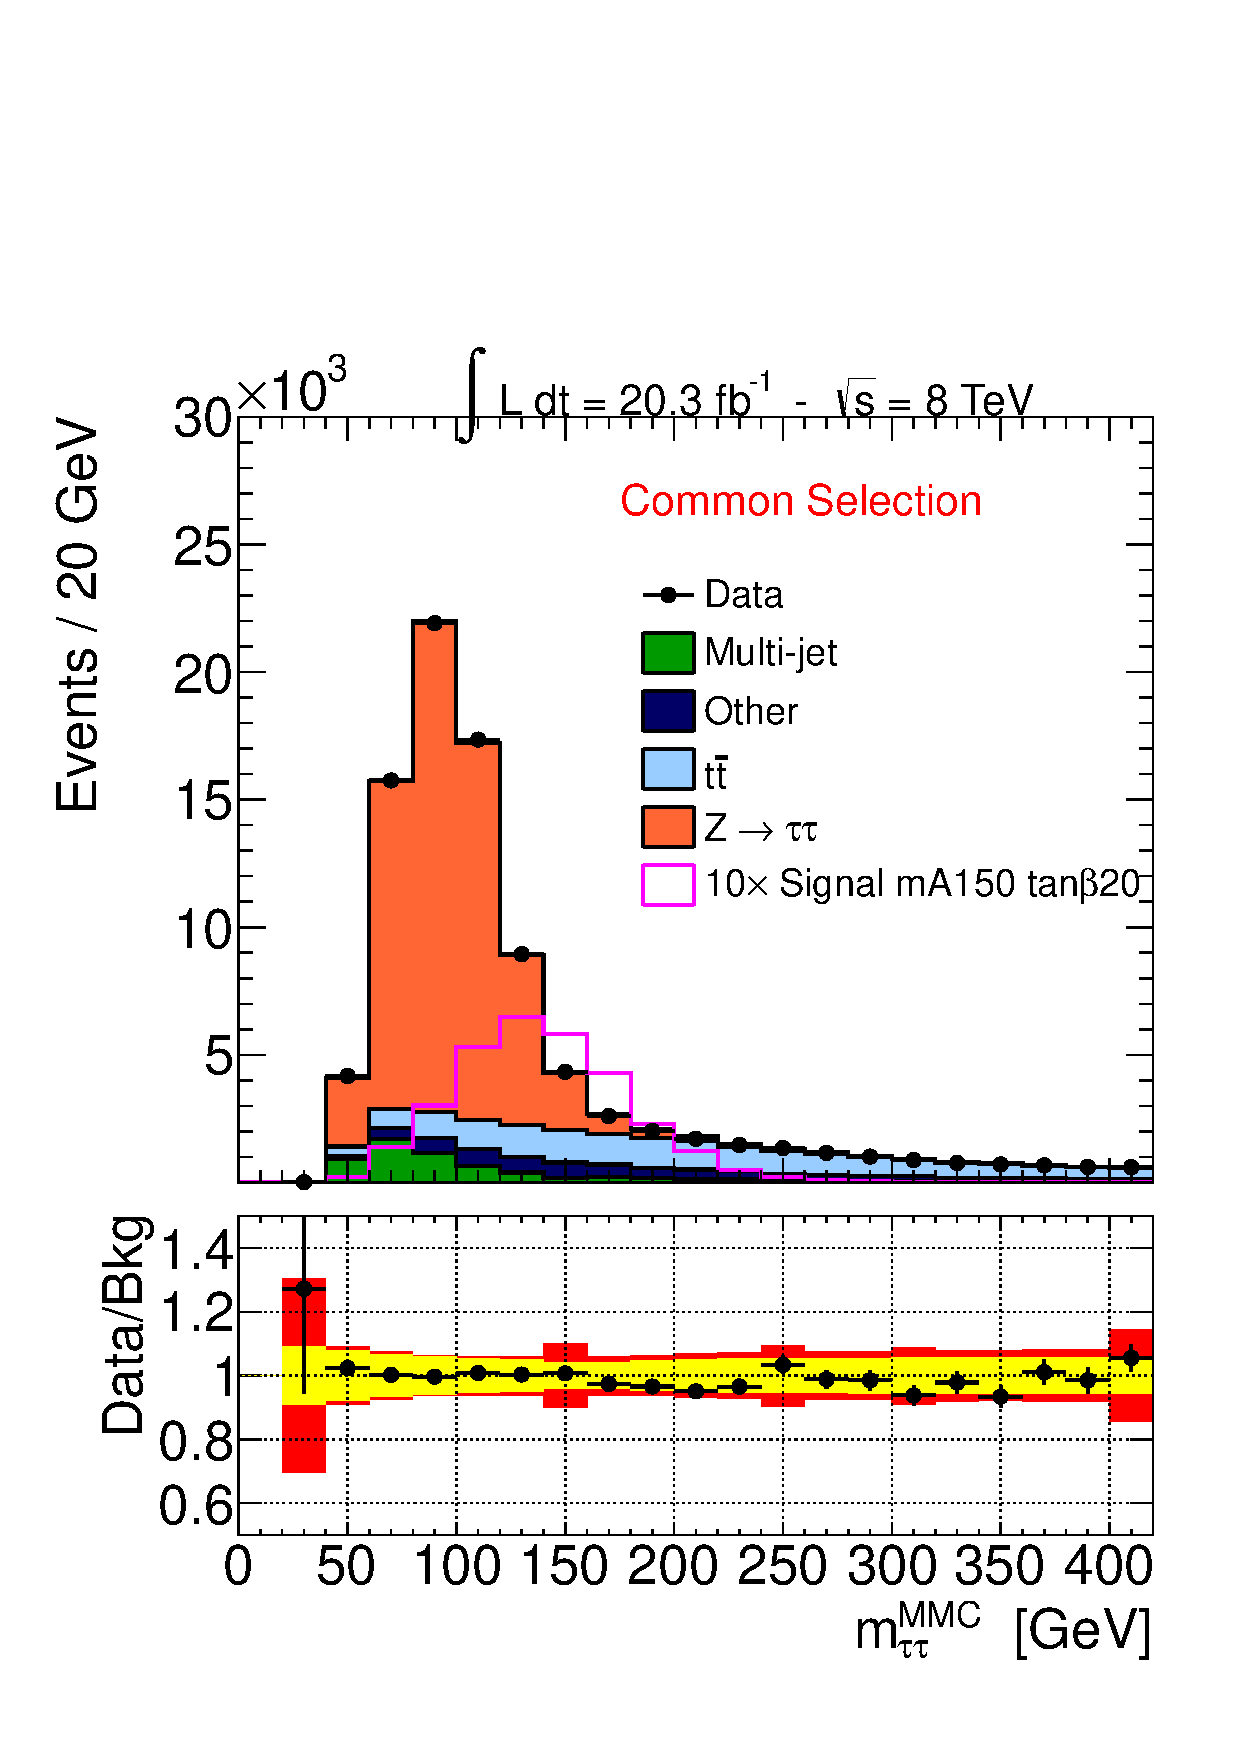
\includegraphics[page=1,width=0.47\textwidth]{figure/final_plots/presel_total_final.pdf}
            %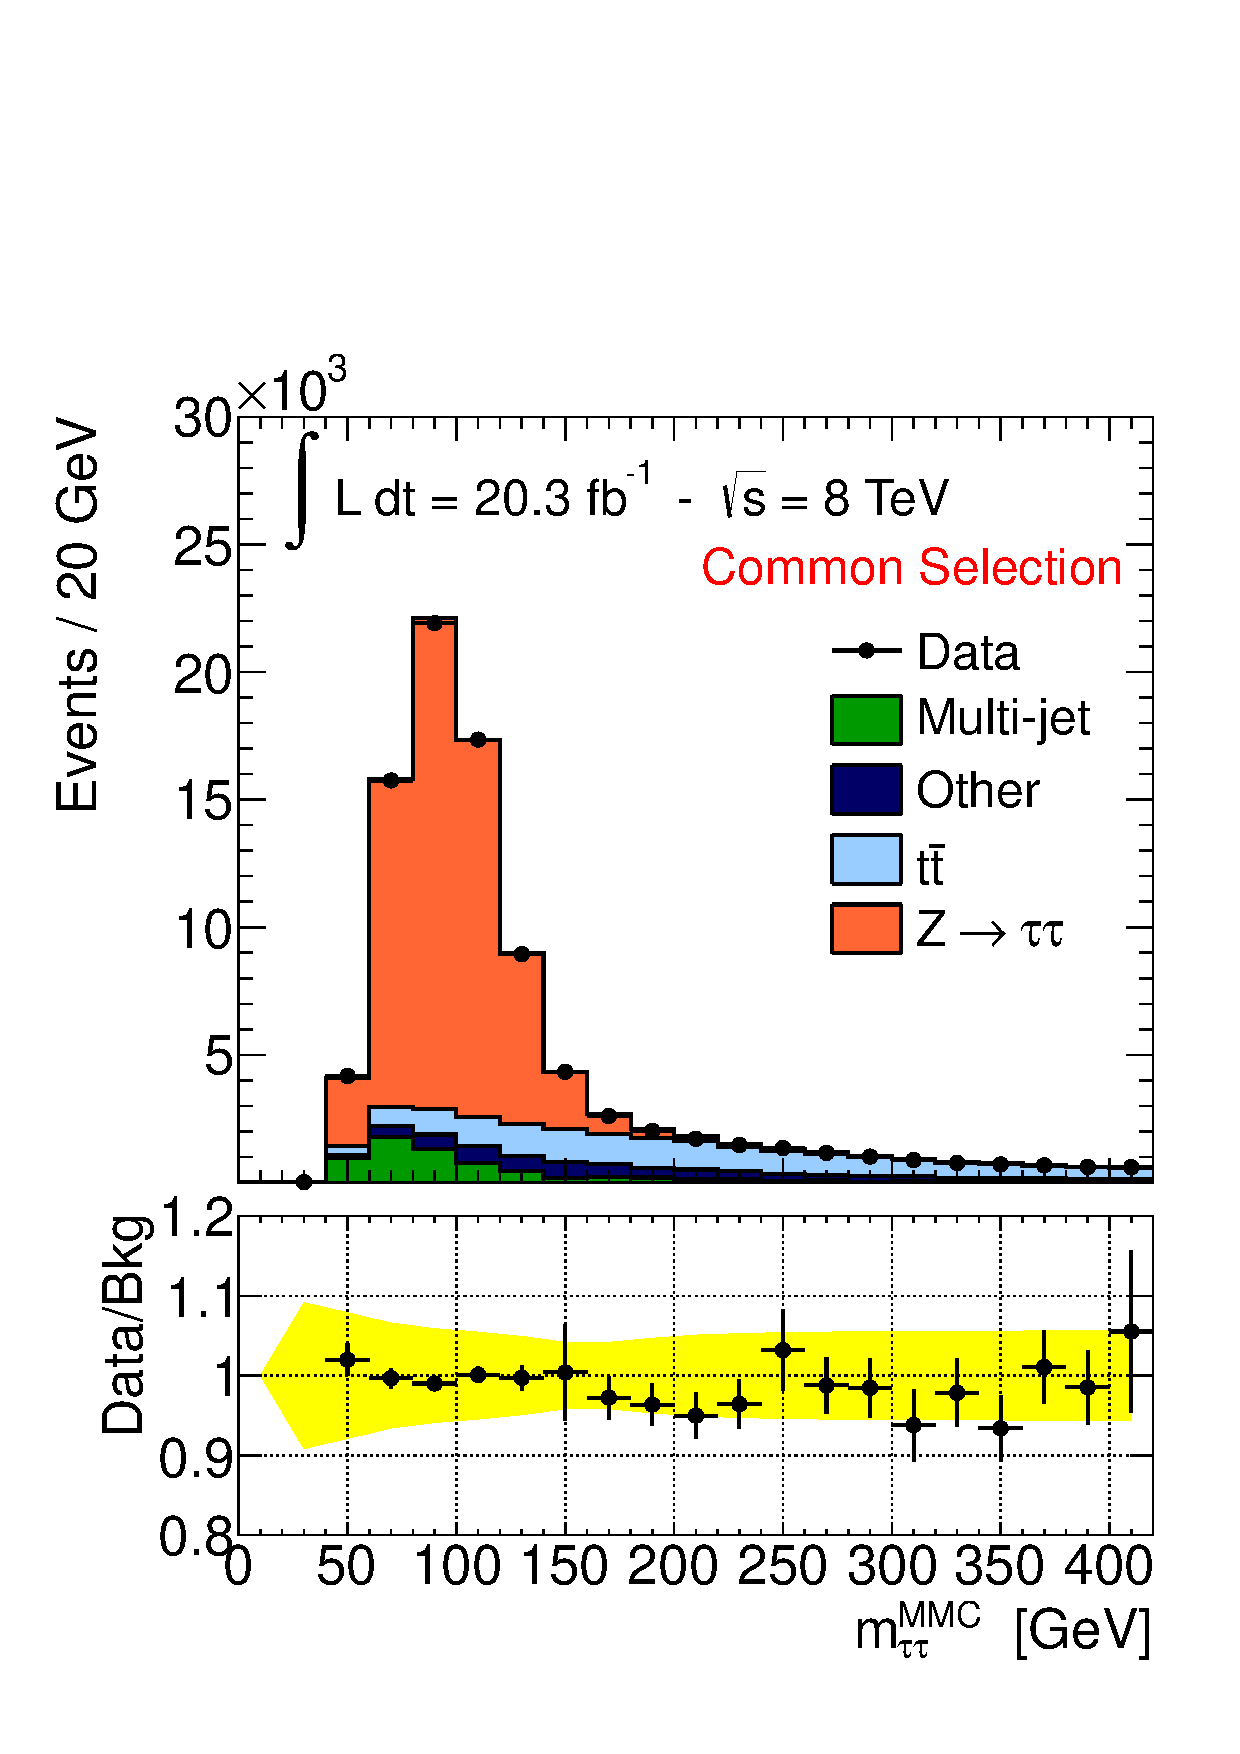
\includegraphics[width=0.47\textwidth]{figure/final_plots/std_presel_mmc_mass.pdf}
     }	
     \subfigure[]{		
            \includegraphics[page=17,width=0.47\textwidth]{figure/final_plots/presel_total_final.pdf}
            %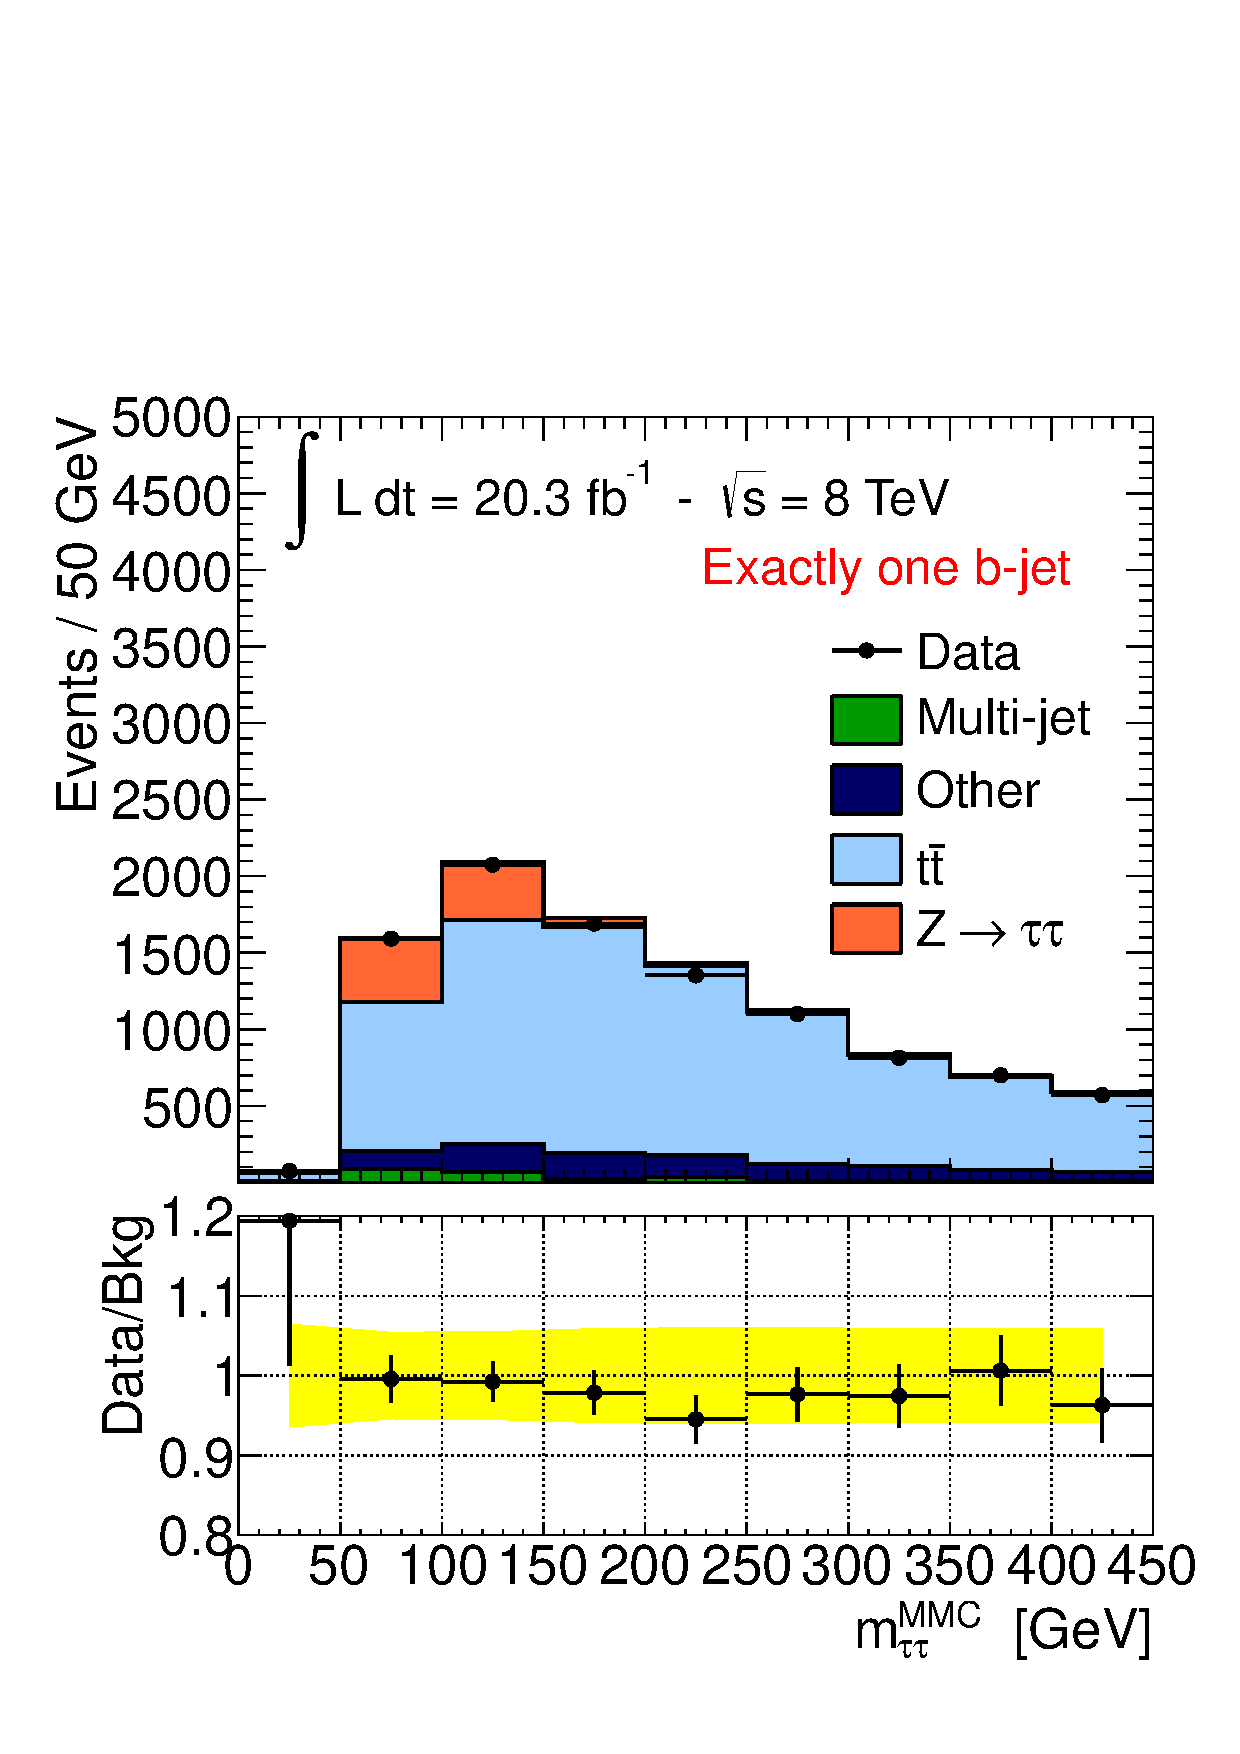
\includegraphics[width=0.47\textwidth]{figure/final_plots/std_presel_Btag_mmc_mass.pdf}
     }	
     \subfigure[]{		
            \includegraphics[page=2,width=0.47\textwidth]{figure/final_plots/presel_total_final.pdf}
            %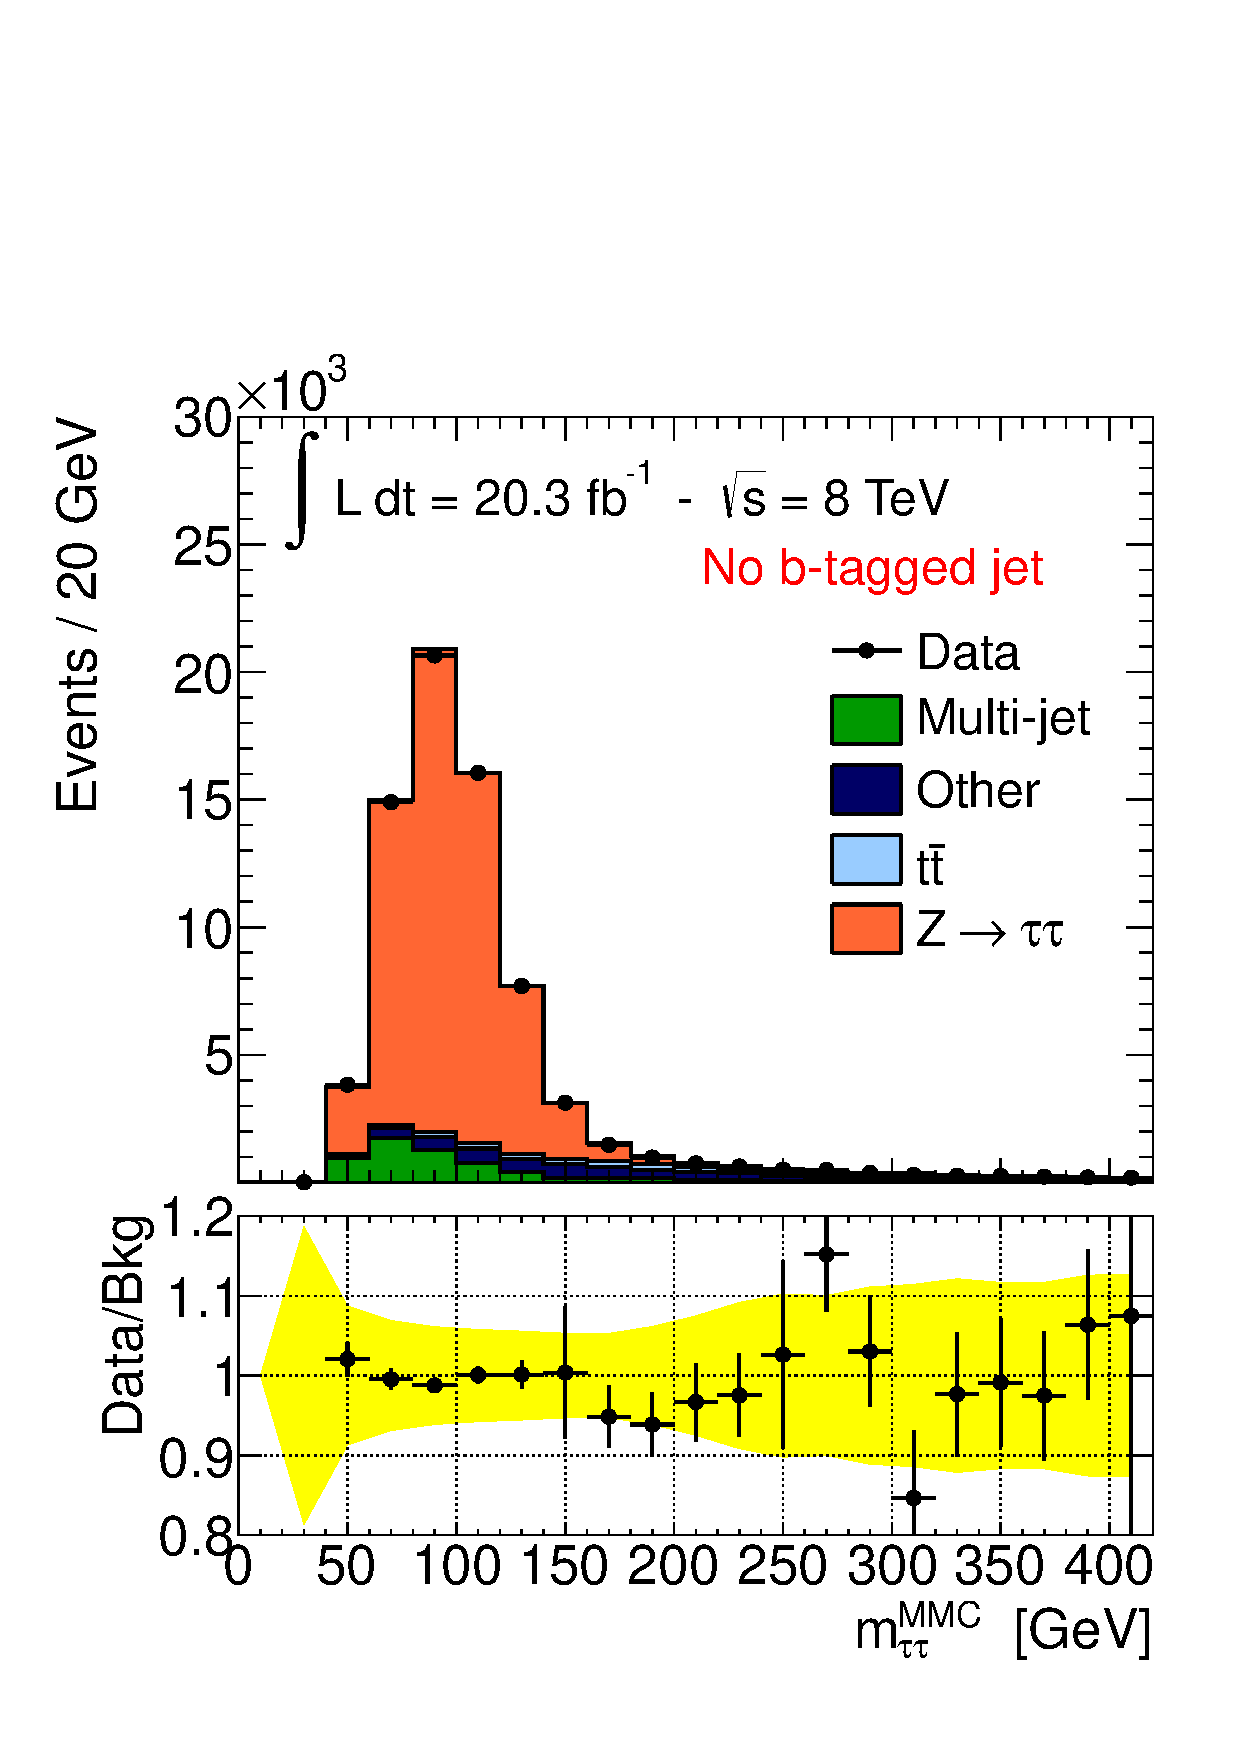
\includegraphics[width=0.47\textwidth]{figure/final_plots/std_presel_NoBtag_mmc_mass.pdf}
     }	
%     \subfigure[]{		
%            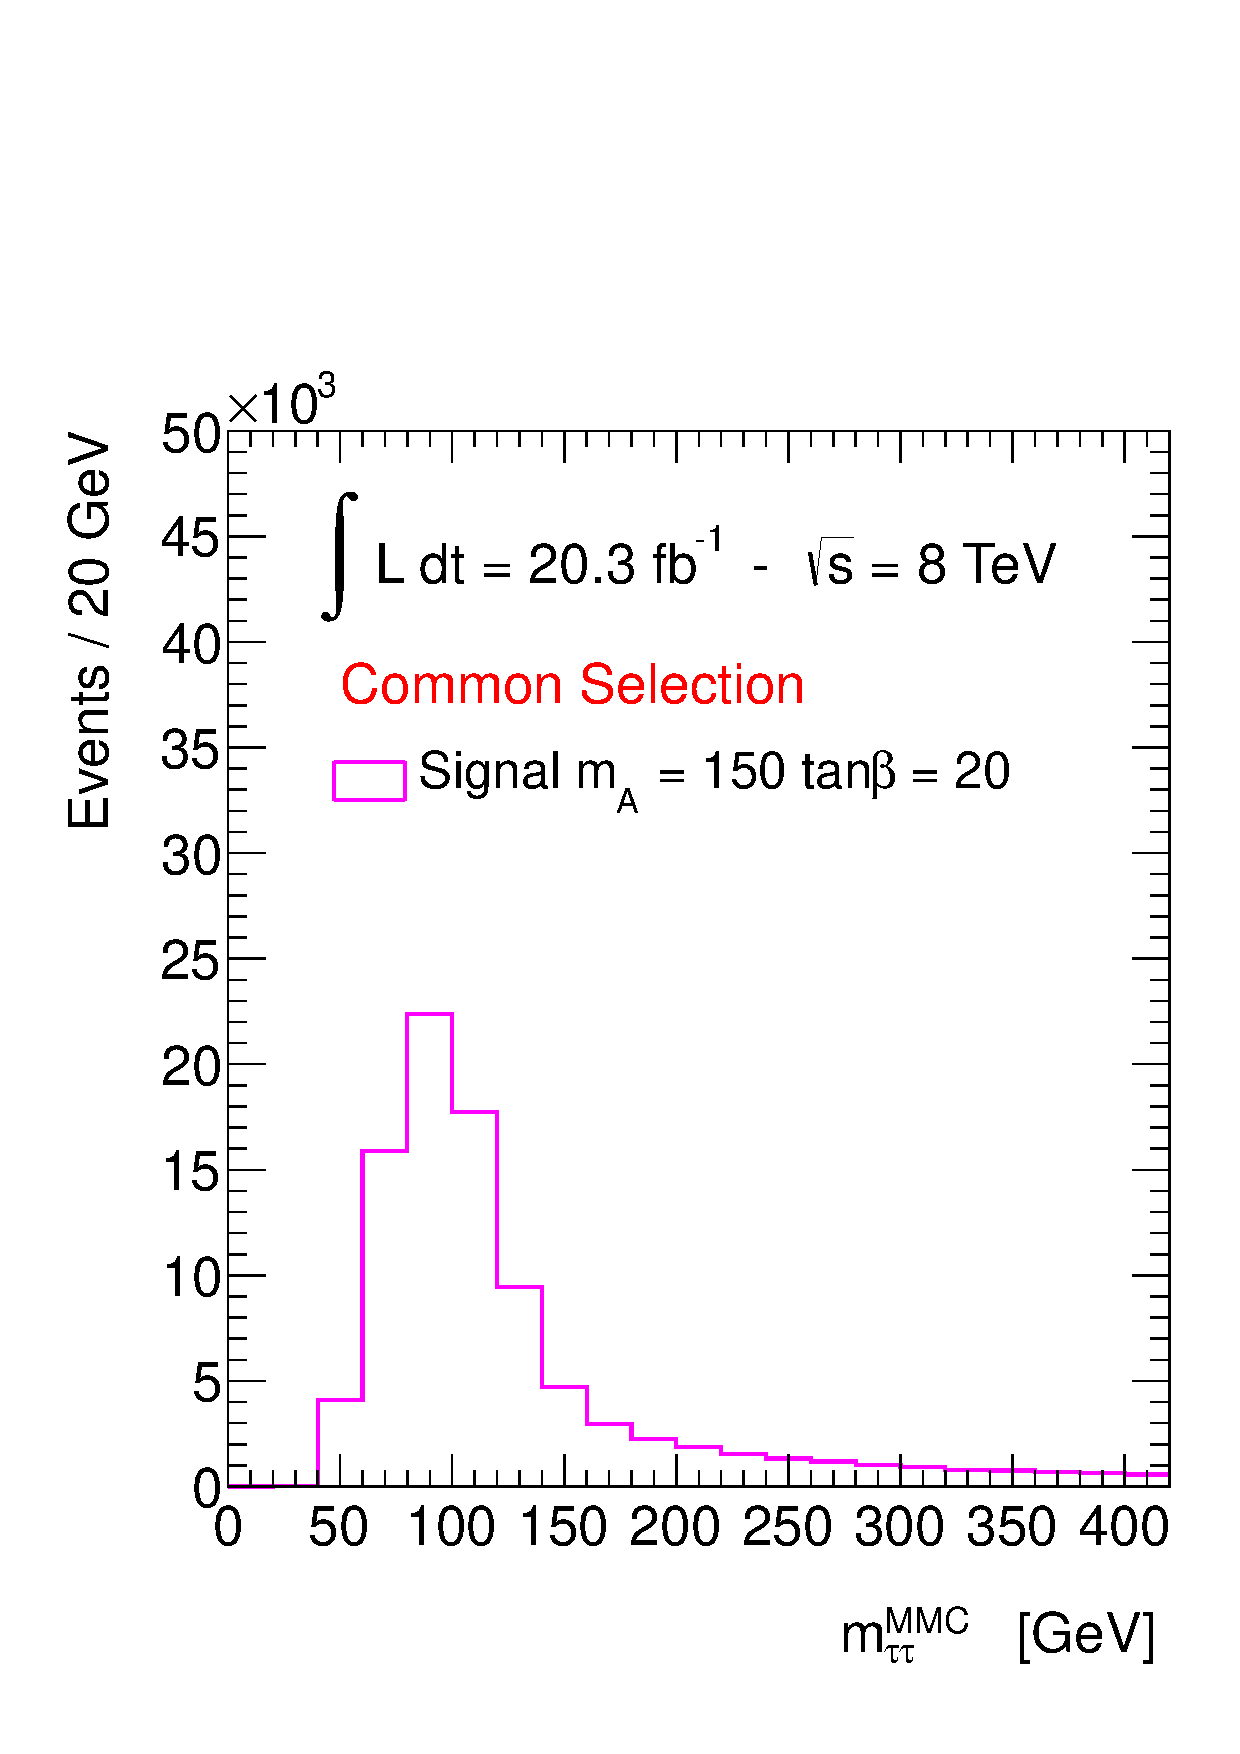
\includegraphics[width=0.47\textwidth]{figure/final_plots/signal_presel.pdf}
%     }	

    \end{center}
     	

    \caption{Observed and expected distribution of the 	invariant di-$\tau$ mass estimate \mmc at
	 different stage of the analysis: (a) after the common selection,
	(b) after requiring exactly one b-tagged jet and (c) for the b-vetoed sample.	The predictions 
	of the  background model is compared to  the data (as in Figure~\ref{fig:selections}).}
   \label{fig:mass}
\end{figure}


The accuracy of the  invariant mass obtained with the \mmc method depends strongly on the 
resolution of the missing transverse energy measurement.
To improve the $\met$ resolution, a scan of a six-dimensional parameter space is performed 
in a similar manner as described above. For this purpose, the absolute value of $\vec{E}_T^{miss}$ is also considered unknown and a scan 
is performed over all possible values constrained by the measured $\met$ and its corresponding uncertainty.
%on it assigning values  according to its uncertainty. 
%The probability of each solution is calculated and the final missing transverse
%energy is given by the weighted mean of the scanned points. 
%
%The final procedure consist in obtaining first an estimate for $\met$ by means of a six dimensional scan over the solution of equations~\ref{eq:MMC},
%successively a four dimensional scan is performed fixing $\met$ to the updated value and calculating the most likely invariant mass 
%of the di-$\tau$ system.

Figure~\ref{fig:mass} shows the  \mmc invariant mass distribution after the common selection and after the 
event categorisation.

 
%Accurate invariant mass reconstruction of a di-tau system is a challenging task due to the escaping neutrinos.
%In this analysis, with four neutrinos in the final state, the number of unknown largely exceed the number of constraints,
%several approximation are possible to further constraint the neutrinos, for example assuming them collinear to the 
%other leptons from tau decay, however those approximation suffers of limitations. 

%In this analysis we use the so called missing mass calculator (MMC)~\cite{MMC}
%technique for the calculation of the di-tau system invariant mass. This technique employs additional 
%information from the well known tau decay to constraint the system, this is achieved by minimising a likelihood function 
%defined in the kinematically allowed phase space region, the result is a more precise measurement of the di-tau 
%system invariant mass and a considerable improvement in resolution. The invariant mass distribution 
%calculated with the MMC technique is referred in the following as $\mmc$ and is used as discriminating 
%variable in the limits setting.


\section{Background Modeling and Validation}
\label{sec:BackgroundEstimation}

In this section we make use of analysis tools and object definition
(like electrons, jet or muon) described in chapter~\ref{c:detector}.
Monte Carlo (MC) Simulation of the background and signal processes is extensively
used that are used to model the backgrounds are described in section~\ref{}.
Monte Carlo simulations of any process are usually prone to systematics
uncertainties due to non-perfect descriptions of pileup effects,
underlying event and detector performance, when possible, data-driven 
techniques are employed to estimate backgrounds from data. In particular for the following cases:
\begin{itemize}
  \item[$\bullet$] The $Z \rightarrow \tau\tau \rightarrow ll ~ + ~  4\nu$ is estimated from data using the embedding technique described in Section~\ref{sec:data_mc}.
  \item[$\bullet$] The multi-jet background is estimated completely from data using the so-called ABCD method.   
\end{itemize}
Other background processes, such as \ttbar, single top, dibosons, $Z
\rightarrow ll$ + jets (where $l = e,\mu$) and W + jets, are estimated
using MC predictions and are validated in control regions where possible. Systematic uncertainties on such predictions 
are detailed in Section~\ref{sec:Systematics}.

\subsection{Simulated Event Samples}
\label{sec:SimSamples}

Both the signal and background process modelled by Monte Carlo (MC)
simulation were produced within the ATLAS MC12a production campaign.
The generators used for the different processes are described below.

Signal production via the gluon fusion process, $gg\rightarrow A/H/h$,
was simulated with POWHEG~\cite{POWHEG} and the associated
$b\bar{b}A/H/h$ production with SHERPA~\cite{SHERPA}.  The
pseudoscalar Higgs boson samples were generated in the mass range from
90~GeV to 400~GeV and 90~GeV to 300~GeV for $ggH$ and $b\bar{b}A$
production, respectively, and at $\tan\beta = 20$. The same kinematics
are assumed for $A/h/H$ Higgs bosons decay products and at other
$\tan\beta$ values. Appropriate reweighting is applied according to the
different cross-sections. The $m_h^{\mathrm{max}}$ MSSM benchmark
scenario~\cite{MSSMmhmax} is assumed.

The production of $W$ and $Z/\gamma^*$ bosons in association with jets
was simulated with the ALPGEN~\cite{Alpgen} generator. This employs
the MLM matching scheme~\cite{MLM} between the hard process,
calculated with leading-order matrix elements for up to five jets, and
the parton shower.  The $t\bar{t}$ process was generated using the POWHEG generator. The single-top (s-channel, $Wt$)
processes were generated using MC@NLO~\cite{MCatNLO}, while single-top
(t-channel) processes were generated with AcerMC~\cite{AcerMC}.  The
production of diboson~($WW$, $WZ$, $ZZ$) were generated with
HERWIG~\cite{Herwig}.  For all ALPGEN and MC@NLO samples described
above, the parton shower and hadronisation were simulated with HERWIG
and the activity of the underlying event with JIMMY~\cite{JIMMY}.
%The loop-induced $gg\rightarrow WW$ processes were generated using gg2WW~\cite{GG2WW}.  We are not using it Xsec very small
Different parton density functions (PDFs) sets are used depending on
the generator - CTEQ6L1~\cite{CTEQ6} is used by ALPGEN and AcerMC while
CT10~\cite{CT10} is used by SHERPA, POWHEG and MC@NLO. 

The cross-sections of
the MC event samples used in this note are summarised in
Table~\ref{tab:MCxsec}. The $W/Z$+jets and $b\bar{b}A/H/h\rightarrow \tau\tau$ cross sections are calculated to NNLO. Those for $\ttbar$ are calculated at NLO with resumation of NNLL soft gluon terms. The single top and diboson cross sections are calculated at NLO for single top and dibosons. Finally, the direct $gg\rightarrow A/H/h\rightarrow \tau\tau$ signal cross sections 
are calculated at NNLO and NLO for the top loop and the bottom loop and top/bottom loops interference, respectively.

The values of the steering parameters used for the HERWIG, JIMMY and PYTHIA
generators are described in Ref.~\cite{ATLASMC09Tune}.
TAUOLA~\cite{TAUOLA} and PHOTOS~\cite{PHOTOS} are used to model the
tau lepton decay and additional photon radiation from charged leptons
in the leading-log approximation, respectively, except for SHERPA
samples.  

All MC event samples were passed through the full simulation
of the ATLAS detector using GEANT4~\cite{Geant4,ATLASSIM} and are
reconstructed with the same software version as used for data. The effects of the 
simultaneous recording of several events from the
same or neighbouring bunch crossings (pile-up) are considered in the
simulation. Differences between the simulated and actual LHC running
conditions have been corrected for by re-weighting the simulated
events according to the distribution of the average number of
interactions per bunch crossing ($<\mu>$) obtained from the ATLAS
data.

  
\begin{table}[htdp]
\begin{center}
\caption{The cross sections (multiplied by the relevant branching
  ratios~(BR)) used in this note. Signal cross sections are shown for $m_A=150$~GeV and $\tan\beta=20$
\label{tab:MCxsec}
}
\begin{tabular}{cc}
\\
\hline \hline
Process                                                                 & Cross-section~(pb) [$\times$ BR] \\ \hline
$W\rightarrow \ell$+jets ($\ell=e, \mu, \tau$ )                          & 12.22$\times 10^3$ \\
$Z/\gamma^{*}\rightarrow \ell\ell$+jets ($m_{\ell\ell}>60$ GeV)      & 1.15$\times 10^3$ \\
$Z/\gamma^{*}\rightarrow \ell\ell$+jets ($10<m_{\ell\ell}<60$ GeV) & 4.35$\times 10^3$ \\
$t\bar{t}$                                                              & 137.3 \\
Single top $t$-, $s$- and $Wt$-channels                                 & 28.4, 1.8, 22.4 \\
Diboson WW, WZ and ZZ                                                  & 20.6, 6.8, 1.55 \\ \hline
Signal ($m_A=150$~GeV, $\tan\beta=20$, $m_{h}^{max}$ scenario)   &  \\ \hline
$gg\rightarrow A\times$BR$(A\rightarrow\tau\tau)\times$BR$(\tau\tau\rightarrow e\mu+ 4\nu)$                 & $ 16.8 \times 0.118 \times 0.062$ \\
$gg\rightarrow H\times$BR$(H\rightarrow\tau\tau)\times$BR$(\tau\tau\rightarrow e\mu+ 4\nu)$ ($m_H=151$~GeV) & $ 18.4 \times 0.119 \times 0.062$ \\
$gg\rightarrow h\times$BR$(h\rightarrow\tau\tau)\times$BR$(\tau\tau\rightarrow e\mu+ 4\nu)$ ($m_h=129$~GeV) & $ 13.7 \times 0.110 \times 0.062$ \\
$b\bar{b}A\times$BR$(A\rightarrow \tau\tau)\times$BR$(\tau\tau\rightarrow e\mu + 4\nu)$                       & $ 39.4 \times 0.118 \times 0.062$ \\
$b\bar{b}H\times$BR$(H\rightarrow \tau\tau)\times$BR$(\tau\tau\rightarrow e\mu+ 4\nu)$ ($m_H=151$~GeV)       & $ 35.7 \times 0.119 \times 0.062$ \\
$b\bar{b}h\times$BR$(h\rightarrow \tau\tau)\times$BR$(\tau\tau\rightarrow e\mu+ 4\nu)$ ($m_h=129$~GeV)       & $ 4.71 \times 0.110 \times 0.062$ \\
\hline \hline
\end{tabular}
\end{center}
\end{table}


\subsection{Top Quark Pair Production Validation}
\label{sec:top_est}

The background from top quark pair production is estimated using a sample of events from the POWHEG-PYTHIA MC
generator. To validate this MC sample,  a \ttbar rich control region is defined using events passing the preselection described in section \ref{sec:eventpresel} with the additional requirement of two b-tagged jets.
%Since this is one of the major backgrounds for this analysis (especially in b-tag category)
%a careful validation of this background model is need, for this purpose a  top quark enriched control region (CR)  
%is defined by adding to the preselection the further requirement of exactly two b-tagged jets in the event. 
Figures~\ref{fig:kinematicsttbar} and~\ref{fig:cutsttbar} show a set of kinematic and analysis selection
variables in this CR, for both data and the MC prediction. A good agreement between data and the background model is found.
%and shows that our top-quark background model describes well the data
The prediction of the event yield in this CR is in good agreement with data: an overall
data to background ratio of $0.998 \pm 0.011\mathrm{(stat.)} \pm 0.110 \mathrm{(sys.)}$ is observed. The total systematic uncertainty on the ratio is dominated by the uncertainty on the b-tagging scale factors. In addition, this result could be used
as a measure of $t\bar{t}$ normalisation avoiding systematic uncertainty on the theoretical cross section of
this process. In this case, however, additional acceptance systematics would need to be evaluated in a dedicated study.
%
%with a dedicated RIVET analysis and uncertainties of the order of the cross section 
%uncertainty are expected, we then drop this possibility considering that wont bring  
%significant improvements.

\begin{figure}[htp]
     \begin{center}

        \subfigure[]{%MMC
            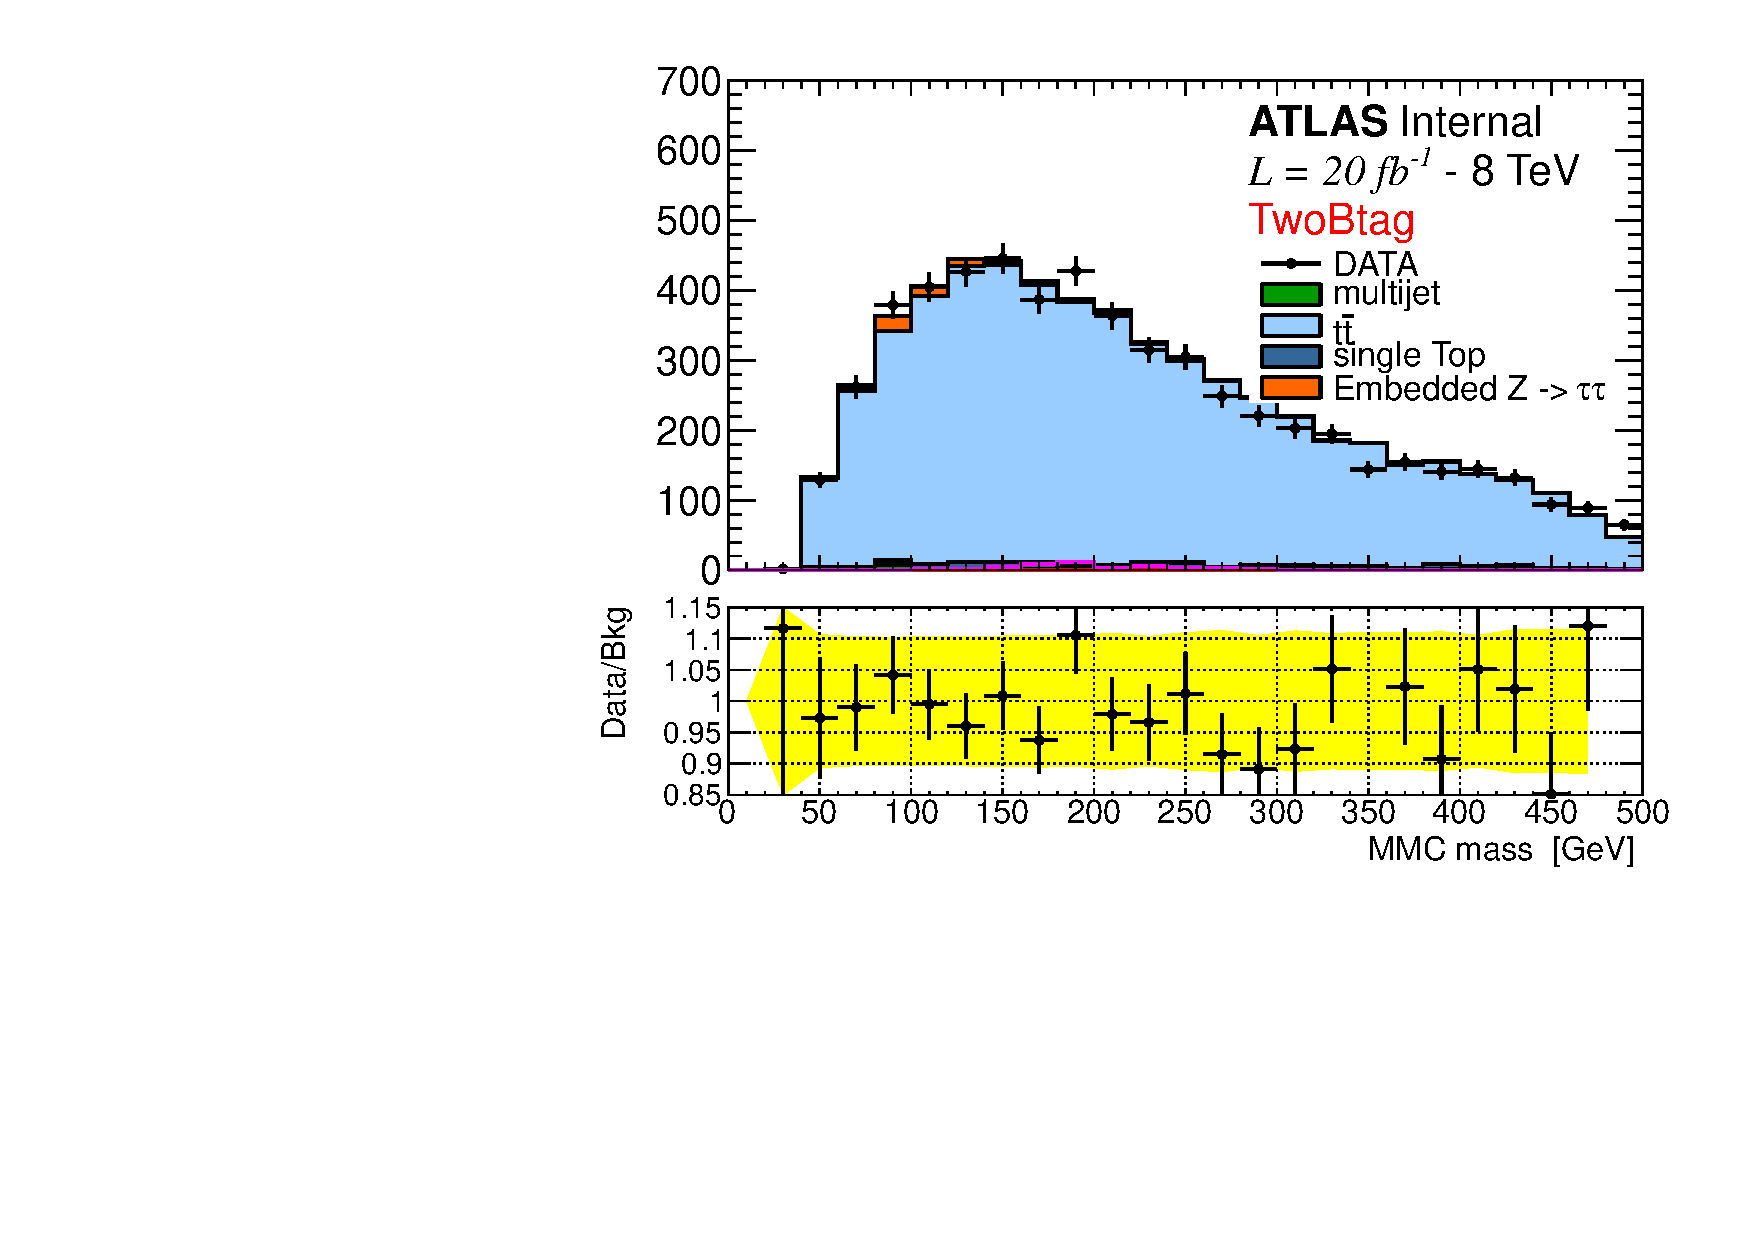
\includegraphics[page=1,width=0.45\textwidth]{figure/bg_estimation/std_plots_twoBtag.pdf}
        }
        \subfigure[]{%ele pT
           \includegraphics[page=6,width=0.45\textwidth]{figure/bg_estimation/std_plots_twoBtag.pdf}
        } 
        \subfigure[]{%Muon pt
            \includegraphics[page=8,width=0.45\textwidth]{figure/bg_estimation/std_plots_twoBtag.pdf}
        }

    \end{center}
    \caption{ Distributions  of a) the MMC mass, b) the transverse momentum of the electron $\pt(e)$ and c) the transverse momentum of the muon $\pt(\mu)$, for both data and MC in the \ttbar control region. The uncertainties on the points for the ratio plot show the statistical uncertainty on the data to background ratio, whereas the yellow band show the total systematic uncertainty on this ratio.} 
   \label{fig:kinematicsttbar}
\end{figure}


\begin{figure}[ht!]
     \begin{center}

        \subfigure[]{
            \label{fig:cuts_a} %DPhi
            \includegraphics[page=12,width=0.45\textwidth]{figure/bg_estimation/std_plots_twoBtag.pdf}
        }
        \subfigure[]{%CosDphi
            \label{fig:cuts_b}
            \includegraphics[page=13,width=0.45\textwidth]{figure/bg_estimation/std_plots_twoBtag.pdf}
        }\\
        \subfigure[]{%Ht
            \label{fig:cuts_c}
            \includegraphics[page=10,width=0.45\textwidth]{figure/bg_estimation/std_plots_twoBtag.pdf}
        }
        \subfigure[]{%Lep+Et
            \label{fig:cuts_d}
            \includegraphics[page=11,width=0.45\textwidth]{figure/bg_estimation/std_plots_twoBtag.pdf}
        }

    \end{center}
    \caption{Distributions of a) $\Delta\phi(e-\mu)$,
      b) $\sum\cos\Delta\phi$, c) \SumLtMET and d) \Ht , for both data and MC in the \ttbar control region. The uncertainty on the points for the ratio plot show the statistical uncertainty on the data to background ratio, whereas the yellow band show the total systematic uncertainty on this ratio.}
   \label{fig:cutsttbar}
\end{figure}


\subsection{Multi-jet Background}
\label{sec:qcd}

The QCD multi-jet background represents an important background, 
especially in the b-veto category, due to its high cross-section and the 
relatively low cut on lepton \pt used in this analysis. This
background is evaluated by a data-driven technique, the so-called ABCD method.
The ABCD method consists of splitting the data sample in four regions: the
 signal region (SR) and three control regions (CR), where the control
regions are mutually orthogonal and designed to be enriched in
multi-jets events. The four regions are defined by using the charge correlation
between the leptons and the isolation cuts used in the lepton preselection. 
To obtain regions rich in multi-jet background, the selections on both
the calorimetric and tracking isolation are inverted with respect to the
nominal ones described in Section~\ref{sec:eventsel}. Hence it is
possible to define four regions: opposite sign (OS) or same sign
(SS) with respectively isolated or anti-isolated leptons. Historically
the letters A-D are assigned to this regions for a quicker reference as
defined in Table~\ref{table:qcd}.

\begin{table} [ht]
\centering
\begin{tabular}{c c c }
\hline
Region & Lepton Charge & Lepton Isolation \\ [0.5ex]
\hline
A (signal region) & OS & isolated \\
B & SS & isolated \\
C & OS & anti-isolated \\
D & SS & anti-isolated \\ [1ex]
\hline
\end{tabular}
\caption{QCD background estimation control regions, defined by having leptons with opposite signs (OS) or same signs (SS) and by having the leptons either isolated or anti-isolated.}
\label{table:qcd}
\end{table}

An assumption of the ABCD method is that multi-jet backgrounds
populate the OS and SS events independently of lepton isolation
criteria and hence that the ratio of OS/SS events is uncorrelated 
with the lepton isolation selections. In this case, the number of QCD events in the signal region $A$ 
can be estimated from the yield of multijet events in the control regions $B$, $C$ and $D$, using the equation
\begin{equation} \label{eqn:qcdest}
N_{A}  = N_{B} \times \frac{N_{C}}{N_{D}} =  N_{B} \times \rqcd
\end{equation}
%Here is  assumed that the events in the control regions come solely from QCD multi-jet processes, contamination
%from electroweak (W and Z + jets, dibosons) and top processes
%($t\bar{t}$ and single top production) are  subtracted in each control region 
%using the MC prediction for their event yield.  
To obtain the multijet yields in the data CRs, the contamination
from electroweak (W+jets, Z+jets and dibosons) and top processes
($t\bar{t}$ and single top production) are  subtracted in each control region 
using the MC prediction for their event yield.  Tables~\ref{table:qcd_yield_btag}~and~\ref{table:qcd_yield_bveto}
show the event yield
% in the b-tagged and b-veto categories, respectively,
for each CR throughout the full cut-flows, along with the
predictions of non-QCD multi-jets events which are subtracted.
Signal contamination has been checked in all the three control regions for different 
mass points. For the range of $m_{A}$ and $\mathrm{tan}\beta$ considered in this analysis, the highest signal contamination 
is seen in region B for the mass point $m_{A} = 300$ GeV, where at $\mathrm{tan}\beta = 50$ a contamination 
of 0.2\% is observed. This value is mainly due to b-associated production and,
as it scales with the cross section, for $\mathrm{tan}\beta = 20$ would be an order of magnitude smaller.

Shapes of kinematic distributions for QCD events are taken from the
control region B, even though this region suffers from lower statistics than either region C or D.
This choice is made to avoid a shape bias due to the trigger:  an isolated trigger is used for electrons (as described in Section~\ref{sec:eventsel}), where the offline requirement equivalent to this trigger choice is $\ptcone20/\pt <0.1$.
Figure~\ref{fig:BvsD} shows the comparison between the electron \pt~ distributions in isolated and anti-isolated events, both for SS control regions. Here high \pt~ electrons are suppressed due to isolation requirement of the the trigger. 
Eventually the trigger isolation requirement could
bias also the ratio OS/SS - this possibility has been checked carefully
in a dedicated study and reported in Appendix \ref{appendix:qcd}.
To a good approximation, such trigger effects cancel out in the ratio
OS/SS, so no systematic is applied to the ratio because of this.

To test the ABCD method predictions an additional control region has been defined with the following selections:
\begin{itemize}
\item \MET $< 20$ GeV
\item \Ht $< 70$ GeV and \SumLtMET$ < 50$ GeV
\item $0 < \mmc < 80$ GeV  	 
\end{itemize}
%{\bf This control region is designed to enhance multi-jet background with respect to \Ztautau.}
Figure~\ref{fig:ABCD_cr} shows the \mmc distribution for this region with and without b-tagging requirements. 
Agreement between data and the background model is found in this control region within statistical and 
detector related systematics uncertainty. 

\begin{figure}[tp]
	\begin{center}
	\includegraphics[width=9cm]{figure/ABCD_regionB_Vs_regionD}
	\end{center}
	\caption{Comparison of the electron \pt~distribution in region B and region D, showing the bias due to the trigger. 
	The histograms are normalised to the same area.}
	\label{fig:BvsD}
\end{figure}
%%%%	this table is not that useful

%\begin{table} [p]
%	\caption{Contribution to the different control regions from non-QCD background, after the preselection. }
%	\centering
%	\begin{tabular}{ c c c c c c c}
%%%%%%%%%%%%%%%%%%%%%%%%%%%%%%%%%%%%%%%%%%%%%%%%%%%%%%%%
%\hline
%Region  &  \Ztautau	 & $t\bar{t}$	 & W + jets	 & $Z \rightarrow ll$ + jets & Single Top 	& Dibosons \\ [0.5ex]
%\hline
%  B 	& 341 	$\pm$ 6	&	700$\pm$ 11	&	3398$\pm$ 180	& 830 $\pm$ 58	     &	178$\pm$ 8 		&   612$\pm$ 10  \\
%  C 	& 16 	$\pm$ 2	&	719$\pm$ 12	&	409$\pm$ 50	& 17 $\pm$ 4	     &	103$\pm$ 6		& 13$\pm$ 1 \\
%  D 	& 8	$\pm$ 2	&	539$\pm$ 10	&	49$\pm$	12	& 24$\pm$  7	     &	67$\pm$	 4		& 6$\pm$ 1 \\[1ex]
%\hline
%%%%%%%%%%%%%%%%%%%%%%%%%%%%%%%%%%%%%%%%%%%%%%%%%%%%%%%
%	\end{tabular}
%	\label{table:qcd_mc}
%\end{table}


%%%%%%%%%%%%%%%%%%%%%%%%%%%%%%%%%%%%%%%%%% PUT FINAL NUMBERS!!!!!!!!!!!!!!!! %%%%%%%%%%%%%%%%%%
\begin{table} [p]
	\begin{tabular}[c]{l r c c c c}
%%%%%%%%%%%%%%%%%%%%%%%%%%%%%%%%%%%%%%%%%%%%%%%%%%%%%%
\hline 
\hline 
Selection  &  		& B & C  & D &  \rqcd \\
\hline
Preselection 	&   Data	&6189			&604628			&312901		    &	1.929 $\pm$  	0.004		\\
	        &   non-QCD	&2510 $\pm$  180  	&1090 $\pm$   30  	&730	$\pm$ 35    &				\\
\hline
B-tag	     	&   Data	&419		&44619 			&27257		    &	1.64	$\pm$	0.01	\\
	     	&   non-QCD	&215 $\pm$  10	&310 $\pm$	12	&277 	$\pm$ 13    &				\\
\hline
$\Delta\phi(e-\mu)$  &   Data		&230		&38810 			&23316		    &	1.67	$\pm$	0.01	\\
	     &   non-QCD	&104 $\pm$ 6	&200 $\pm$	10	&175	$\pm$ 7	    &				\\
\hline
$\sum\cos\Delta\phi$ &   Data & 149		&31379 			&18779		    &	1.67	$\pm$	0.02	\\
	     &   non-QCD      & 67 $\pm$ 5	&127 $\pm$	8	&114 $\pm$	6   &				\\
\hline
$\sum H_T$ &   Data	      & 83		& 27781 		&15626		    &	1.78	$\pm$	0.02	\\
	&   non-QCD	      & 23 $\pm$  4	& 25 $\pm$	3	& 22 $\pm$   3	    &				\\ 
\hline
\SumLtMET &   Data	&71		&27735 	&15590		    &	1.78	$\pm$	0.02	\\
	     &   non-QCD	 & 10 $\pm$	3	& 22  $\pm$ 3		&18	$\pm$ 2	    &			\\
\hline
$\mmc > 0.$    &  Data	& 70	& 27634 	& 15522		    			    &	1.78	$\pm$	0.02	\\
	     &   non-QCD	& 9 $\pm$ 3	& 20  $\pm$ 3		&17	$\pm$ 2	    &			\\[1ex]
\hline
\hline
%%%%%%%%%%%%%%%%%%%%%%%%%%%%%%%%%%%%%%%%%%%%%%%%%%%%%%
	\end{tabular}
	  \caption{QCD background estimation as a function of the analysis selections for the b-tagged category. The yields for the different control regions, as well as the scaling factor \rqcd, are reported. The error on the \rqcd is statistical only.}
	\centering
	\label{table:qcd_yield_btag}
\end{table}


\begin{table} [p]
	\begin{tabular}[c]{l r c c c c}
%%%%%%%%%%%%%%%%%%%%%%%%%%%%%%%%%%%%%%%%%%%%%%%%%%%%%%%
\hline
\hline 
Selection  &  		& B & C & D &  \rqcd \\ 
\hline
Preselection 	&   Data	&6189			&604628			&312901		    &	1.929 $\pm$  	0.004		\\
	        &   non-QCD	&2510 $\pm$  180  	&1090 $\pm$   30  	&730	$\pm$ 35    &				\\
\hline
B-veto	     	&   Data	&5673		  & 558217 		& 284847		    &	1.960	$\pm$	0.004	\\
	     	&   non-QCD	&2220	$\pm$ 180 & 710 $\pm$ 30	& 415 $\pm$	30	    &				\\
\hline
$\Delta\phi(e-\mu)i$  &   Data		&4610		&532583 		&271404		    	    &	1.962	$\pm$	0.005	\\
	     &   non-QCD	&1700 $\pm$170	&580 $\pm$	30	& 345 $\pm$	30	    &				\\
\hline
$\sum\cos\Delta\phi$ &   Data& 3417	&486747 		& 247712	   		    &	1.965	$\pm$	0.005 	\\
	     &   non-QCD     & 1120  $\pm$ 100	& 370 $\pm$ 	20		& 230 $\pm$	20  &				\\
\hline
$\mmc > 0.$    &  Data		& 3177		& 479967 		& 244276	    	    &	1.965	$\pm$	0.005	\\
	     &   non-QCD	& 1000 $\pm$ 100	& 300  $\pm$ 17		&190	$\pm$ 20    &			\\[1ex]
\hline
\hline
%%%%%%%%%%%%%%%%%%%%%%%%%%%%%%%%%%%%%%%%%%%%%%%%%%%%%%%
	\end{tabular}
	\caption{QCD background estimation as a function of the analysis selections for b-veto category. The yields for the different control regions, as well as the scaling factor \rqcd, are reported. The error on the \rqcd is statistical only.}
	\centering
	\label{table:qcd_yield_bveto}
\end{table}



\begin{figure}[tp]
	\begin{center}
	     
	\subfigure[]{
		\includegraphics[page=1,width=0.49\textwidth]{figure/QCD/qcd_CR_emb.pdf}
	        }
	\subfigure[]{
  	\includegraphics[page=5, width=0.49\textwidth]{figure/QCD/qcd_CR_emb.pdf}
	}
	
	\end{center}
	\caption{\mmc distribution for QCD cross check regions defined in section \ref{sec:qcd} (a) and for the same CR when in addition one b-tagged jet is required (b). }
	\label{fig:ABCD_cr}
\end{figure}


Systematic uncertainties are assigned on the scaling factor \rqcd and on the shape of
the discriminating variable \mmc to take into account any correlation between isolation and charge 
of the leptons, details on the systematic uncertainty evaluation are addressed in Section~\ref{sec:Systematics}.

\subsection{$Z \rightarrow \tau\tau$ + Jets Background}
A good understanding of the background from \Ztautau decays is vital to this
analysis. Unfortunately, for a light Higgs boson, it is impossible to completely separate \Ztautau decays 
from the signal - hence a signal free data control region cannot be defined.
However, thanks to the small Higgs coupling to muons, \Zmumu decays provide a good starting point to 
model \Ztautau events in a data-driven way. Hence a hybrid Data-MC sample, known as "Embedding" is used to model the \Ztautau background: 
$\Zmumu$ candidates are selected in data, then the two muons from the $Z$ decay are substituted with the decay 
products from simulated taus, those taus have the same kinematics as the original muons. 
Further details may be found in \cite{Embedding, SMold}.

%The selection of the \Zmumu input data requires exactly two combined, opposite charged
%muons, where the leading muon has a transverse momentum $\pt > 20 \GeV$ and 
%the subleading muon $\pt > 15\GeV$. Both muons are requited to lie within $|\eta|<2.5$ and to be isolated with 
%$\ptcone 20/\pt<0.2$ (see Section~\ref{sec:presel}). Additionally 
%the invariant mass of the two muons is required to be in the range $M_{\mu\mu} > 40$ GeV.
%Once the muon pair events are selected, all tracks and calorimeter cells associated to the muons are 
%removed from the \Zmumu data event. Finally, the calorimeter cell energy and tracks from the simulated tau decays
%are added to the data event and the event is re-reconstructed.

%A set of corrections are applied to correct for the muon trigger efficiency, the muon reconstruction efficiency and other additional effects
%related to the original \Zmumu events. Finally, as the trigger is not emulated in the embedding sample, 
%an additional correction is applied to emulate the electron and muon trigger efficiencies in the final \Ztautau embedded events. 
%For a full description of the corrections and validation see \cite{SMnew}.

The Embedding technique, which uses \Zmumu decays to 
model \Ztautau events in a data-driven way, is described in Section~\ref{sec:data_mc}. 
As there is no simulation of the trigger in the embedding samples, the event yield
is normalised to ALPGEN \Ztautau at preselection stage. Furthermore a set of corrections, as described in \cite{SMnew}, are
applied to account for the trigger and muon reconstruction efficiency in the original \Zmumu events, to emulate the trigger efficiency in the embedded \Ztautau events and to correct for the b-layer requirements that are not modelled in the embedded events.

The Embedding technique has been validated in several studies, detailed in~\cite{Embedding, SMnew}, which show a good description of 
data and \Ztautau MC by \Ztautau events from Embedding. In the context of this analysis, figures~\ref{fig:emb_vs_alp1} and \ref{fig:emb_vs_alp} show comparisons of various kinematic variables between
data, embedding and ALPGEN \Ztautau events at preselection. No significant deviation is seen between the \mmc distribution of the embedding and ALPGEN samples (here the data \mmc distribution is not shown). However other relevant variables for this analysis, such as the \MET and the number of b-jets, are slightly better described by embedding. Additional plots are reported in appendix~\ref{appendix:additionalEmb}.

\begin{figure}[tp]
     \begin{center}

            \includegraphics[page=1, width=0.6\textwidth]{figure/bg_estimation/std_plots_emb.pdf}
\end{center}
    \caption{Comparison between the embedded \Ztautau and ALPGEN for $\mmc$ distributions.}
   \label{fig:emb_vs_alp1}
\end{figure}


\begin{figure}[tp]
     \begin{center}

           \includegraphics[page=2, width=0.6\textwidth]{figure/bg_estimation/std_plots_emb.pdf}
            \includegraphics[page=3, width=0.6\textwidth]{figure/bg_estimation/std_plots_emb.pdf}

    \end{center}
    \caption{Comparison between embedded \Ztautau and ALPGEN for $\MET$ and the number of b-tagged jets distributions.
	Data are superimposed, with the contribution of non-\Ztautau are subtracted.}
   \label{fig:emb_vs_alp}
\end{figure}


%plot comparing embedding and ALPGEN Et miss and b-tagging, data -MC not Ztautau and compare data alp and emb.

As the embedding sample is based on selecting \Zmumu candidates in data, the selections assure a rather 
pure \Zmumu sample. However further selections used in this analysis, for example the b-tagging requirements, 
could enhance the contamination fraction from other processes in the embedding sample. Hence dedicated studies have been
made to estimate the $t\bar{t}$ and QCD multi-jet contamination in the embedding sample.
The \ttbar~ contamination is estimated by evaluating the embedding sample yield in a two b-tag control region,
as described in Section~\ref{sec:top_est}. These events are assumed to be solely from $t\bar{t}$
and their yield in the signal region is extrapolated using POWHEG-PYTHIA $t\bar{t}$ simulation sample.
Table~\ref{table:emb_cont_tt} shows a summary for the top contamination in embedding and this contamination is hence taken to be negligible. The multi-jet contamination can be estimated starting 
from the embedding yield of opposite sign anti-isolated events (region C).
%one should not use SS regions because embedding already requires leptons to be OS, then would be biased
Assuming all events in this CR as QCD multi-jet events, the contamination in the SR 
can be estimated using the ABCD method (see Section\ref{sec:qcd}). The \rqcd factor 
used in this case is evaluated using a mu-mu final state CR with the same kinematics selections
used in the definition of the embedding sample. Table~\ref{table:emb_cont_qcd}
shows the estimated contamination of QCD multi-jet in embedding. 
We  consider contamination effects negligible.

\begin{table} [p]
\centering
\begin{tabular}{c c c c c}
\hline
\hline
 & Embedding yield in CR & Transfer factor & Estimated events in SR & Contamination \\ [0.5ex]
\hline
b-tag & $84 \pm 9$  & $(2.6 \pm 0.1) \times 10^{-2}$ &  $2.2 \pm 0.2$&  0.5 \% \\
b-veto & $84 \pm 9$ & $(1.74 \pm 0.02) \times 10^{-1}$ & $15 \pm 2$ & 0.03 \% \\[1ex]
\hline
\end{tabular}
\caption{Evaluating embedding $t\bar{t}$ contamination using a two b-tag CR. The transfer factor is the
multiplicative factor that allows to estimate events in SR from the CR. }
\label{table:emb_cont_tt}
\end{table}

\begin{table} [tp]
\centering
\begin{tabular}{c c c c c}
\hline
\hline
 & Embedding yield in CR & Transfer factor & Estimated events in SR & Contamination \\ [0.5ex]
\hline
B-tag  & $12 \pm 3$ & $ (7 \pm 1) \times 10^{-3}$ &  $(8.4 \pm 0.3) \times 10^{-2}$ &  0.03 \% \\
B-veto & $390 \pm 20$ & $(2.5 \pm 0.1) \times 10^{-2}$ & $10.0 \pm 0.5$ & 0.02 \% \\[1ex]
\hline
\end{tabular}
\caption{Evaluating embedding contamination due to QCD multi-jet using ABCD method, 
the CR here is with OS anti-isolated events (region C). The transfer factor is the
multiplicative factor that allows to estimate events in SR from the CR, in this case is $N_{B} / N_{D}$
and is evaluated using mu-mu final state with the same kinematic selection used in the 
definition of the embedding sample. }
\label{table:emb_cont_qcd}
\end{table}


\section{Systematic Uncertainties}
\label{sec:Systematics}

This section describes the range of systematic uncertainties
that are relevant for this analysis. To account for differences in the detector responses between simulation and data a 
set of corrections are applied either at object reconstruction level, as described in section~\ref{sec:presel}, or at the event level. 
The uncertainties on such corrections are considered as detector-related systematic uncertainties and are detailed in section~\ref{sec:sys:sys_det}. Further systematic uncertainties related to data-driven methods for backgrounds estimation
are described in section~\ref{sec:sys_bg}.  For
samples which rely on MC simulation, theory-related
systematics, which include uncertainties on the cross-section and
uncertainties on the acceptance of analysis selections,  
are finally described in section~\ref{sec:sys_theory}.

Each single systematic can contribute separately to the uncertainty on the
final event yield and on the shape of the $\mmc$
distribution that is used as the discriminating variable for the limit derivation. These shape systematics are
documented in appendix~\ref{appendix:shapeNPs}. Systematic uncertainties that do not effect the
mass shape distribution and have an impact on the event yield of a samples of less than 0.5\% are 
neglected in the final limit calculations.
%hey infact do not have any significant effect on the final expected limits.


\subsection{Detector-related Systematics Uncertainties}
\label{sec:sys:sys_det}

%Here we address systematic uncertainty related to object reconstruction and event 
%corrections, those correction are based on the measure of some relevant parameter, each of those parameter correspond 
%to a "nuissance paremeter" in our probability model as described in Section~\ref{sec:ExclusionLimits}.
%
%Reciepe:
%
%Correction are measured elsewhere, those correspond to property of the object like 
%energy scale or resolution, or are related to event properties like pieleup ecc.., along with theyr mean value
%an uncertainty is evaluated,
%We variate each parameter independently (one sigma up or down) according with their uncertainty and evaluate the impact on the analysis yield for each sample. An intepolation algorithm then defines what is the impact of that nuissance parameter
%on the analysis for any value. In the following we describe in detail the uncertainties on each used correction,
%table~\ref{tab:ExpSys:btag} and~\ref{tab:ExpSys:bveto} briefly summarize the impact on the samples yield for the most significant systematic uncertainty considered. 



\paragraph{Luminosity}
The uncertainty on the integrated luminosity is taken to be 2.8\% \cite{luminosity}.

\paragraph{Pileup}
As described in Section~\ref{sec:SimSamples}, MC events are re-weighted according to reproduce the average interactions per bunch crossing, $<\mu>$, seen in data. It has been seen
that a proper description of the minimum bias vertex multiplicity is obtained if the $<\mu>$ 
value in MC is first scaled by a factor of $1.11 \pm 0.03$ before re-weighting to match data. The uncertainty
on this value is taken as a systematic uncertainty for the analysis.

\paragraph{Trigger Efficiency}
The scale factors used to correct for the differences in trigger efficiency between data and MC for the triggers considered in this analysis are described in Section~\ref{sec:presel:TriggerCorr}. The uncertainties on these scale factors are used to estimate the systematic uncertainty due to the understanding of the trigger efficiencies. 
Systematic uncertainties on both the single electron and
electron-muon trigger efficiency are considered independently, by varying the scale factors coherently by their uncertainties.
The uncertainties are aproximately 1-2\%, depending on the $\pt$ and $\eta$ of the leptons.

In the embedding sample, the trigger is emulated by applying weights to the event
topology. In addition, corrections are applied to correct for trigger efficiency in the original $\Zmumu$ events. 
These corrections are likewise varied coherently by their uncertainties to estimate the trigger systematic uncertainty 
for this background. Hence, the trigger systematic uncertainty for embedding is considered independently
from that for the other backgrounds.

\paragraph{Electrons}
Two types of uncertainty on reconstructed electron objects are considered:
the first are related to electron identification and reconstruction efficiencies, respectively. 
The second type are related to electron energy scale and resolution corrections.
The effect of the uncertainties on the reconstruction and identification is estimated by coherently varying the applied scale factors by their 
associated uncertainties. The effect on the final yield of each sample from both of the uncertainties is then 
summed in quadrature to give the overall uncertainty (referred to as "Electron SF").
The energy scale uncertainties are split into a set due to six different nuisance parameters \cite{EGammaEnergy}. 
However many of them are found to have a negligible effect on the overall yield. Only the uncertainties 
related to the $Z \rightarrow ee$ measurement ("Electron Zee") 
and due to low momentum electrons ("Electron LOWPT") are found to give a significant effect. Both of these two uncertainties affect the mmc mass distribution, in particular for 
\Ztautau samples, hence these are considered as shape systematics in the limit calculation.
We sum in quadrature all the other uncertainties related to energy scale and resolution (referred as "Electron E.").
%PUT IN APPENDIX OR HERE PLOTS OF SHAPE

\paragraph{Muons}
The uncertainty on muon identification efficiency depends on the charge and momentum of the muon.
Typically these uncertainties are of the order of a fraction of percent, and are referred as "Muon ID". 
The uncertainties on the muon momentum are considered by smearing  the inner detector and muon spectrometer \pt~ 
values and changing the \pt~ scale within their uncertainties. 
Each component is varied individually and the individual variations in event yields 
summed in quadrature. The total systematic uncertainty is referred to here as "Muon E.".

\paragraph{Taus}
Hadronic tau object are only used in the analysis as a veto. Uncertainties on both tau energy scale 
and identification efficiency have been investigated and are found to be negligible for this analysis.

\paragraph{Jets}
The systematic uncertainties on the Jet Energy Scale (JES) are split up into multiple sets of nuisance parameters, which
 hence contain a full treatment of the bin-by-bin correlations of the uncertainties. The overall uncertainty on the JES ranges 
 between 3\% and 7\%, depending on the $\pt$ and $\eta$ of the jet. The recommendation \cite{TWIKI_JETMET} to propagate each individual 
 source of uncertainty through the full analysis is followed. In this analysis the reduced set of fourteen uncertainties, know as 
 \verb=InsituJES2012_14NP=, have been considered: these include two uncertainties for eta intercalibration, four pile-up 
 uncertainties, a high-$\pt$ uncertainty and an uncertainty for MC non-closure. Of these, only the terms "JES Effective 1", 
 "JES Effective 2" and "JES Effective 3", the pileup uncertainty as a function of the number of primary vertices ("JES Pileup-NPV") and the uncertainty due to the jet area ("JES Pileup-Rho") have a significant effect on the event yields. Additionally, 
 the uncertainty related to the fraction of quark to gluon jets ("JES Flav. Comp") and on the different response to them ("JES Flav. Resp.") are considered. The additional uncertainty assigned to the b-jet energy scale, referred as "JES B", is also 
 significant to this analysis. Uncertainties related to theory and modelling ("JES EtaModelling") also contribute to this 
 analysis. Finally the effect of the jet energy resolution ("JES Resolution") is evaluated applying a smearing to the jets, the 
 resulting effect on the yield is symmetrised.

\paragraph{b-Tagging}
Uncertainties on the knowledge of both the b-tag and mistag efficiencies for the 70\% working point of the MV1 b-tagger are
 considered in this analysis. Hence both the b-tag and b-veto channels are affected. The tag and mistag efficiencies are
  considered to be totally anti-correlated. Uncertainties for b-quark, c-quark and light or gluon initiated jets, referred to as 
  "B  Eff.", "C Eff." and "L Eff." respectively, are considered. In the rare case where a hadronically decaying 
  tau is b-tagged, the uncertainty for c-quark induced jets is used.


\paragraph{Missing Transverse Energy}
In addition to propagating the effect of the energy scale
uncertainties for all the physics objects to the \met, the effect of
uncertainties on the ``soft-terms'' of the \met are
considered. Uncertainties on both the scale and resolution of the
soft-terms are independently propagated through the analysis and are
added in quadrature, this final term is referred as "MET" uncertainty.


\paragraph{Summary} A summary of the effect of the experimental and theoretical systematic uncertainties on signal and background yields for the b-tag and b-veto channels are shown in Table~\ref{tab:ExpSys:btag} and Table~\ref{tab:ExpSys:bveto}, respectively. It should 
be noted that the gluon fusion  signal sample suffers of poor statistics in the b-tag category. 
Hence, some of the yield differences reported are statistically dominated for these samples.
%	As a solution the mean value between all the sample mass point can be taken as measure of the single systematic, 
However the gluon fusion production mode has a negligible contribution in b-tag category.
	
\begin{table}[hp]
  \centering
  \begin{tabular}{lccccc}
    \hline\hline
      	      		   \multicolumn{6}{c}{ b-tag category uncertainties (\%)}  \\
     \hline
      Source             & Signal bbH & Signal ggH & \Ztautau &  Top 	& Other	 \\
    \hline
Electron SF  		 &2.3		   &2.0		     &	2.8    &	1.8	&2.0	 \\
Electron E.	  	 &0.7		   &1.2		     &0.5	     &0.5	&0.9	 \\
Electron LOWPT	  	 &0.4		   &0.0		     &0.4	     &0.1	&0.4	 \\ 
Electron Zee	  	 &0.3		   &0.6		     &0.4	     &0.6	&0.5	 \\
Muon ID 		 &0.3		   &	0.3	     &	0.3	     &	0.3	&0.3	 \\
Muon E.		  	 &0.5		   &7.7		     &0.1	     &0.1	&0.2	 \\
Trigger Single	Ele.  	 &0.7		   &0.5		     &0.5	     &0.8	&0.8	 \\
Trigger Dilepton	  	 &1.0		   &1.2		     &1.4	     &0.6	&0.6	 \\
Embedding MFS	  	 &-		   &-		     &0.0	     &-		&-	 \\
Embedding Iso.	  	 &-		   &-		     &1.3	     &-		&-	 \\
JES Effective-1   	 &0.5		   &0.0		     &-		     &3.8	&2.3	 \\
JES Effective-2   	 &0.6		   &7.8 	     &-		     &5.5	&2.5	 \\
JES Effective-3   	 &0.5		   &0.0		     &-		     &2.2	&2.0	 \\
JES EtaModelling    	 &1.1		   &0.0		     &-		     &4.0	&2.1	 \\
JES Pileup-NPV	  	 &0.5		   &0.0		     &-		     &1.2	&0.3	 \\
JES Pileup-Rho	  	 &0.8		   &7.8 	     &-		     &2.8	&2.2	 \\
JES FlavComp.	  	 &1.2		   &6.3		     &-		     &2.1	&4.5	 \\
JES FlavResp.	  	 &1.3		   &0.0		     &-		     &1.4	&1.9	 \\
JES BJet	  	 &1.2		   &0.0		     &-		     &4.2	&1.2	 \\
JER		  	 &1.4		   &6.3		     &-		     &2.9	&3.0	 \\	%Should be added in Framework	
B Eff		  	 &10.2		   &5.3		     &-		     &2.6	&5.0	 \\
C Eff		  	 &0.2		   &2.8		     &-		     &0.0	&1.2	 \\
L Eff		  	 &0.4		   &8.0		     &-		     &0.1	&1.2	 \\
Pileup			 &0.4		   &0.7		     &0.4	     &0.4	&0.9	 \\		%Should be added in Framework	
MET 		  	 &0.7		   &11.0 	     &0.2	     &1.0	&1.2	 \\
Acceptance		 &		   &		     &		     &		&	  \\
Cross Section	  	 &-		   &-		     &5.0	     &5.5	&7.1	 \\
Luminosity	  	 &2.8 		   &2.8	 	     &2.8 	     &2.8 	&2.8 	 \\

    \hline
    \hline
  \end{tabular}
  \caption{Summary of the effect of the experimental and theoretical systematic uncertainties on the yields of the different
	%samples used  in the b-tag channel. Here "Other" refers to the sum of all the remaining samples: $\Wln$, 
	%diboson, $\Zll$ and single top. The signal samples listed here are b-associated production and gluon 
	fusion with $m_{A}=120$ GeV and $\tan\beta=20$. 
	 Systematic uncertainties with a negligible effect are are listed with a value of 0.0
	 and those that lead to a  shape uncertainty are noted with the symbol (\textbf{s}). 
	Note that the same naming convention is respected for the actual nuisance parameters in the limit framework.}

  \label{tab:ExpSys:btag}
\end{table}


\begin{table}
  \centering
  \begin{tabular}{lccccc}
    \hline\hline
      	      		   \multicolumn{6}{c}{ b-veto category uncertainties (\%)}  \\
     \hline
      Source             & Signal bbH & Signal ggH & \Ztautau &  Top 	& Other	 \\
    \hline
Electron SF  		 &2.4		   &2.3		     &2.9 (\bf{s})	     &1.4	&1.6	 \\
Electron E.	  	 &0.4		   &0.5		     &0.4	     &0.5	&0.9	 \\
Electron LOWPT	  	 &0.3		   &0.5		     &0.4 (\bf{s})	     &0.0	&1.2  \\ 
Electron Zee	  	 &0.4		   &0.4		     &0.4 (\bf{s})	     &0.1	&0.3	 \\
Muon ID 		 &0.3		   &0.3		     &0.3	     &0.3	&0.3	 \\
Muon E.		  	 &0.1		   &0.1		     &0.1	     &0.5	&0.5	 \\
Trigger Single	Lep.  	 &0.6		   &0.6		     &0.5	     &0.9	&0.9	 \\
Trigger Dilep.	  	 &1.0		   &1.0		     &1.3	     &0.2	&0.3	 \\
Embedding MFS	  	 &-		   &-		     &0.1 (\bf{s})	     &-		&-	 \\
Embedding Iso.	  	 &-		   &-		     &0.0 (\bf{s})	     &-		&-	 \\
JES Effective-1   	 &0.2		   &0.2		     &-		     &0.4	&0.4	 \\
JES Effective-2   	 &0.2		   &0.3		     &-		     &0.3	&0.5	 \\
JES Effective-3   	 &0.2		   &0.2		     &-		     &0.2	&0.3	 \\
JES EtaModelling    	 &0.1		   &0.1		     &-		     &0.1	&0.3	 \\
JES Pileup-NPV	  	 &0.3		   &0.1		     &-		     &0.1	&0.3	 \\
JES Pileup-Rho	  	 &0.3		   &0.2		     &-		     &0.5	&0.5	 \\
JES FlavComp.	  	 &0.1		   &0.2		     &-		     &0.2	&0.5	 \\
JES FlavResp.	  	 &0.2		   &0.4		     &-		     &0.3	&0.6	 \\
JES BJet	  	 &0.2		   &0.0		     &-		     &0.5	&0.1	 \\
JER		  	 &0.5		   &0.3		     &-		     &0.6	&0.3	 \\	%Should be added in Framework	
B Eff		  	 &1.8		   &0.0		     &-		     &12.0	&0.8	 \\
C Eff	  		 &0.0		   &0.1		     &-		     &0.1	&0.0	 \\
L Eff	  		 &0.0		   &0.1		     &-		     &0.2 	&0.1	 \\
Pileup			 &0.5		   &0.8		     &0.4	     &0.3	&0.3	 \\	%Should be added in Framework	
MET  		  	 &0.2		   &0.8 	     &0.1	     &0.2	&0.5	 \\
Acceptance		 &		   &		     &		     &		&	  \\
Cross Section	  	 &-		   &-		     &5.0	     &5.5	&5.9	 \\
Luminosity	  	 &2.8 		   &2.8	 	     &2.8 	     &2.8 	&2.8 	 \\

    \hline
    \hline
  \end{tabular}
  \caption{Summary of the effect of the experimental and theoretical systematic uncertainties on the yields of the different
	samples used  in the b-veto channel. Here "Other" refers to the sum of all the remaining samples: 
	$\Wlnu$, diboson, $\Zll$ and single top. The signal samples listed here are b-associated production 
	and gluon fusion with $m_{A}=120$ GeV and $\tan\beta=20$. 
	 Systematic uncertainties with a negligible effect are are listed with a value of 0.0
	 and those that lead to a  shape uncertainty are noted with the symbol (\textbf{s}). 
	Note that the same naming convention is respected for the actual nuisance parameters in the limit framework.}
 \label{tab:ExpSys:bveto}
\end{table}


\subsection{Systematics for Data-Driven Background Estimation Methods} 
\label{sec:sys_bg}

\subsubsection{\Ztautau Embedding Systematics}
An important element of the embedding method is the subtraction of the 
calorimeter cells associated with the muons in the original \Zmumu event and their substitution with those from the simulated tau
decays. To make a conservative estimate of the systematic uncertainty on this procedure, the energy of the subtracted cells is scaled up or down by 30\%. The analysis is repeated with those modified samples and the relative uncertainty is referred as EMB\_MFS. The effect of this uncertainty on the \mmc distribution is shown in figure~\ref{fig:EmbeddingShapeNPs}. Hence the nuisance parameter is treated as a shape uncertainty in the limit machinery.

\begin{figure}[tp]
	\begin{center}
	\includegraphics[width=0.49\textwidth]{figure/systematics/emb_sys_BtagFull_MFS.png}
	\includegraphics[width=0.49\textwidth]{figure/systematics/emb_sys_NoBtagFull_MFS.png}
	\end{center}
	\caption{Embedding MFS systematic uncertainty impact on $\mmc$.}
	\label{fig:EMBMFS}
\end{figure}

%\begin{figure}[htp]
%     \begin{center}
%
%        \subfigure[]{%
%            \label{fig:mvis}
%            \includegraphics[width=0.45\textwidth]{figure/distributions/NP_Shape_EmbMFS_BVeto_mmc.pdf}
%	}
%	
%        \subfigure[]{%
%            \label{fig:mmc}
%            \includegraphics[width=0.45\textwidth]{figure/distributions/NP_Shape_EmbIso_BVeto_mmc.pdf}
%	}
%
%    \end{center}
%    \caption{Effect on the \mmc distribution of the embedding sample due to (a) the EMB\_MFS and (b) embedding isolation systematics. The plots are made after the full b-veto category selection.}
%   \label{fig:EmbeddingShapeNPs}
%\end{figure}

In the selection of the \Zmumu sample only a loose requirement on muon track isolation is required.
A different selection on the muon isolation may effect the selected sample by modifying the topology of the event, % since the requirement is indirectly acting also on the muon \PT, 
changing the non-\Zmumu contamination or the activity in the calorimeter. 
To estimate  the importance of these effects in our
embedding sample, the isolation selection on the muons in the original \Zmumu events is tightened to $\ptcone 40/ \PT<0.06$ and $\etcone 20/ \PT<0.04$, rather than the nominal selection of only $\ptcone 20/ \PT<0.2 $. 
A looser selection would have limited impact because of isolation requirements at trigger level.
The resulting uncertainty, referred to as EMB\_ISO, affects both the yield and the \mmc shape of the embedding samples, as shown in figure~\ref{fig:EmbeddingShapeNPs}. 

Finally, because the normalisation of the embedding sample is determined by the use of the ALPGEN sample, 
we also assign the relative cross section and luminosity uncertainties. In addition
all the detector-related systematic uncertainties relevant to the decay products of the simulated tau 
decay are propagated to the embedding sample.
 
\begin{figure}[tp]
	\begin{center}
	\includegraphics[width=0.49\textwidth]{figure/systematics/emb_sys_BtagFull_Iso.png}
	\includegraphics[width=0.49\textwidth]{figure/systematics/emb_sys_NoBtagFull_Iso.png}
	\end{center}
	\caption{Embedding Isolation systematic uncertainty impact $\mmc$.}
	\label{fig:EMBISO}
\end{figure}

\subsubsection{QCD Multi-Jet Systematics}

In this analysis the QCD multi-jet background is estimated via the ABCD method, as
described in Section~\ref{sec:qcd}. This technique relies strongly on
the assumption that the lepton isolation variables are independent from the
charge correlation between the two leptons. Systematic uncertainties
are assigned to take into account deviations from this assumption.
First we consider the correlation between \rqcd and the lepton isolation selections,
then we compare the result with an auxiliary method. 

Figure~\ref{fig:os_ss_ratio} shows the \rqcd factor, the ratio between the QCD 
yields in region C and D, as a function of the lepton isolation selections (red points).
%correlation is clearly visible. 
As described previously, the expectation from non-QCD backgrounds is subtracted from the data in regions C and D.
To estimate the uncertainty on the value of \rqcd  an additional transfer factor is defined as follows: $R_{QCD}^{iso}  = \hat{A} / \hat{B}$,
where  $\hat{A}$ and $\hat{B}$  are semi-isolated OS and SS regions defined with the lepton isolation larger than the standard requirement, 
but less than a sliding cut. Once more, the non-QCD contributions are subtracted from the data yields.
%$R_{QCD}^{iso}$ is an attempt to calculate a best estimate for the QCD transfer factor between isolated regions,
%which is in definitive the goal of the ABCD method. 
The regions $\hat{A}$ and $\hat{B}$ are chosen to be semi-isolated 
due to the high contamination of non-QCD background and possible signal in region A and B. 
Figure~\ref{fig:os_ss_ratio} shows $R_{QCD}^{iso}$ as a function of the lepton isolation selections (black points).
The difference between \rqcd and $R_{QCD}^{iso} $ in the vicinity of the standard cut value is then assigned as a systematic uncertainty on \rqcd. Using the point where the cuts on the lepton isolation are twice their standard values, a systematic uncertainty of 15\% is found.
The plot in Figure~\ref{fig:os_ss_ratio} is made at preselection level, similar plots using the full selection
for the two categories are in Appendix~\ref{appendix:qcd_additional}.

%for the definition of lepton isolations used in this analysis, the ratio is calculated in regions where the isolation requirements are reversed. Due to a high contamination of signal and non-QCD backgrounds, "semi-isolated" OS and SS regions are additionally defined, where the lepton isolation is larger than the standard requirement, but less than a sliding cut. These regions are labelled $\hat{A}$ and $\hat{B}$  for the semi-isolated OS and SS regions, respectively, and hence we can define $R_{QCD}^{iso}  = \hat{A} / \hat{B}$. The difference between \rqcd and $R_{QCD}^{iso} $ in the vicinity of our standard cut value is then assigned as a systematic uncertainty on \rqcd. Using the point where the cuts on the lepton isolation are twice their standard values, ie. the $x=100\%$ point on the graph, a systematic uncertainty of 15\% is found.

%An additional method considers calculating $\rqcd^{AB}$ as the ratio between the estimated QCD contributions in region A and B.
%These regions, however, suffers of large contribution of non-QCD background and possible signal contamination, 
%this method is then only used as a cross check. Table~\ref{table:MCsub} shows a comparison between \rqcd and  $\rqcd^{AB}$
%for the two category at an early stage of the cutflow where signal contamination is negligible, agreement is seen within statistical uncertainties.

An additional method, used as a crosscheck, considers calculating \rqcd as the ratio between the estimated QCD contributions in region A 
and B. Here the non-QCD contributions are once more subtracted from data. However the large contribution of this non-QCD background, 
along with lack of statistics and possible signal contamination, lead to this only being used as a cross check. Table~\ref{table:MCsub} shows 
a comparison between \rqcd and $\rqcd^{AB}$ for the two categories at the preselection stage of the cutflow, where signal contamination is negligible. 
Agreement is seen between \rqcd values in the two regions, within statistical uncertainties. 

%\footnote{This effect is maybe due to the use of a \PT dependent isolation variable that effects the quark-gluon fraction.}.
%Expectation for non-QCD backgrounds are subtracted as usual. 
%This effect however doesn't tell anything on the uncertainty of our
%measure of \rqcd, we want to measure instead what is the discrepancy (for each
%choosen isolation cut value) between \rqcd and the same factor calculated 
%flipping isolation requirements, i.e. using the isolated regions A and B, we call this factor $R_{QCD}^{iso}$. 
%Due to the high contamination of non-QCD backgrounds and signal in these regions we then define:
%OS and SS isolated regions $\hat{A}$ and $\hat{B}$ in wich the leptons isolation
%should be greather than the standard value but less of predefined quantity on the x axis 
%of the graph (black curve). In definitive we have $R_{QCD}^{iso}  = \hat{A} / \hat{B}$.
%We then assign as a systematics uncertainty the difference between the two curves (red and black) in the vicinity of our
%standard cut value (we use the point where the cut value is doubled, 100\% in the graph because 
%of statistical fluctuation), our estimate of the systematics uncertainty on \rqcd is then 15\%.
%The plot in Figure~\ref{fig:os_ss_ratio} is made at preselection level, similar plots using the full selection
%for the two categories are in Appendix~\ref{appendix:qcd_additional}.

%An additional method used as a crosscheck relies on the definition of "real-$\rqcd$" as the pure ratio between region A and B (non-QCD background
%estimate is subtracted from data in each regions), this would be the exact factor 
%that allows you to extrapolate yield from region B to SR, however it suffer of contamination by non-QCD backgrounds
%and lack of statistics.
%Table~\ref{table:MCsub} shows comparison between \rqcd and real-\rqcd
%for the two category at an early stage of the cutflow where signal contamination is negligible.
%Discrepancies are within statistical uncertainty and underline that an assignment of a  15\%
%uncertainty to the \rqcd factor is conservative.

 %How this is actually implemented in limits machinery
The actual implementation in the limit framework of the ABCD method follows that suggested in~\cite{ABCD}.
Here three free parameters are fitted: number of multi-jet events in region B, $N_{B}^{QCD}$, factor that extrapolates from SS region to OS regions, \rqcd, and the factor that 
extrapolates from isolated to anti-isolated regions $R_{BD}$. Neglecting signal contributions, the following 
equations can be written for the event yield of the B,C and D control regions:
%$$N_{B} = N_{B}^{BKG} + N_{B}^{QCD} $$ 
%$$N_{C} = N_{C}^{BKG} +  N_{B}^{QCD} \times \rqcd \times R_{BD} $$
%$$N_{D} =  N_{D}^{BKG} + N_{B}^{QCD} \times  R_{BD} $$
\begin{itemize}
\item[] $N_{B} = N_{B}^{BKG} + N_{B}^{QCD}$
\item[] $N_{C} = N_{C}^{BKG} +  N_{B}^{QCD} \times \rqcd \times R_{BD} $
\item[] $N_{D} =  N_{D}^{BKG} + N_{B}^{QCD} \times  R_{BD} $
\end{itemize}
where $N^{BKG}$ represent the prediction of  non-QCD background in the relative regions.
The estimate of multi-jet event yield in SR will be then $ N_{B}^{QCD} \times \rqcd $. This method is 
particularly powerful because in the best fit of \rqcd the statistical 
and systematics uncertainty for non-QCD backgrounds and data will be considered.


\begin{table} [tp]
	\begin{center}
	\begin{tabular}{l  c c c }
%%%%%%%%%%%%%%%%%%%%%%%%%%%%%%%%%%%%%%%%%%%%%%%%%%%%%%
\hline 
\hline
Selection  		&  \rqcd  			&  $\rqcd^{AB}$  		&  $R_{QCD}^{iso}$ \\ 
\hline
Preselection 		&   1.929 $\pm$     0.004	&	2.12 $\pm$ 0.17		&	2.22 $\pm$ 0.16	\\
B-veto			&  1.965   $\pm$   0.005    	& 2.10   $\pm$	0.16 		&	2.22 $\pm$ 0.16	\\
B-tag			&  1.78    $\pm$   0.02 	& 1.9   $\pm$	0.9 		&	2.0  $\pm$ 0.8	\\
\hline
\hline
%%%%%%%%%%%%%%%%%%%%%%%%%%%%%%%%%%%%%%%%%%%%%%%%%%%%%%
	\end{tabular}
	  \caption{Comparison between \rqcd, $\rqcd^{AB}$ and $R_{QCD}^{iso}$ for early stage in the cutflow, only b-tag and b-veto
	requirement are applied after preselections. Reported is statistical uncertainty only.}
	\label{table:MCsub}
	\end{center}
\end{table}


\begin{figure}[tp]
	\begin{center}
	\includegraphics[page=5,width=0.9\textwidth]{figure/QCD/qcd_plot.pdf}
	\end{center}
	\caption{OS/SS ratio as a function of lepton isolation variable selections. The selections are varied as a percentage relative to
	the standard lepton isolation cut values (0~in the plot). 
	%As an example the point at 100\% in the plot corresponds
	%to $\rqcd$ evaluated by increasing the isolation requirement by 100\% respect to the standard cut value.
	The red points show the anti-isolated scale factor $\rqcd$, i.e. the ratio between regions C and D.
	 The black points show the isolated SF, which is defined as the ratio between region $\hat{A}$ and $\hat{B}$, 
	 where the leptons have isolation values larger than the nominal value but smaller
	 than the sliding cut on X axis.
%	 taking the same example point at 100\%, than the double of the standard cut value.
	 }
	\label{fig:os_ss_ratio}
\end{figure}

The difference in \mmc shape observed between the OS and SS anti-isolated regions (C and D) is shown in Figure~\ref{fig:qcd_shape_unc}.
This effect is within the  uncertainty on \rqcd of the ABCD method, hence no correction factor is applied to the mass shape. We assume, however, that there could be the same 
shape difference in the isolated regions. Hence a shape uncertainty is assigned in the limit machinery to region B with this deviation. Further 
shape uncertainties due to non-QCD background subtraction are found to be negligible. The uncertainty due to the use of an isolation 
requirement at trigger level is discussed in Appendix~\ref{appendix:qcd} and is found to be negligible.


\begin{figure}[tp]
	\begin{center}
	\includegraphics[width=0.65\textwidth]{figure/QCD/shape_tag.png}
	\includegraphics[width=0.65\textwidth]{figure/QCD/shape_veto.png}
	\end{center}
	\caption{Shape differences for the b-tag and b-veto categories between the ABCD regions C and D.}
	\label{fig:qcd_shape_unc}
\end{figure}

\subsection{Theoretical Uncertainties}
\label{sec:sys_theory}

\subsubsection{Simulated Cross-Section Uncertainties}
Uncertainties on the cross-sections that have been used to normalise
simulation samples to data are reported in
Table~\ref{table:sys_xsec}. These
uncertainties include contributions due to parton distribution
functions (PDFs), the choice of the value of strong coupling constant,
and the renormalisation and factorisation scales.  Furthermore the
uncertainties on signal cross-section depends on $\tan\beta$, the
Higgs boson type ($A$/$h$/$H$) and mass.

\begin{table} [t]
\centering
\begin{tabular}{c c c }
\hline
\hline
Generator & Process & Uncertainty \\ [0.5ex]
\hline
ALPGEN & $Z \rightarrow \tau\tau / ee /\mu\mu$ & $\pm 5\%$ \\
POWHEG & \ttbar					& $\pm 5.5\%$\\
ALPGEN & $W  \rightarrow \tau\nu / e\nu /\mu\nu$&  $\pm  5\%$ \\
AcerMC & single top & $\pm 13 \%$ \\
HERWIG & dibosons & $\pm 6 \%$ \\
SHERPA & $bbA$/$h$/$H$  ($m_{A} \ge 120$~GeV)     & $-(<20)$\%,  $+(<9)$ \%\\
SHERPA & $bbA$/$h$/$H$  ($m_{A} =   110$~GeV)     & $-(<25)$\%,  $+(<9)$ \%\\
SHERPA & $bbA$/$h$/$H$  ($m_{A} =   100$~GeV)     & $-(<28)$\%,  $+(<9)$ \%\\
SHERPA & $bbA$/$h$/$H$  ($m_{A} =    90$~GeV)     & $-(<30)$\%,  $+(<9)$ \%\\
POWHEG & $ggA$/$h$/$H$  ($m_{A} \le 300$~GeV)     & $<$ 15\%\\  [0.5ex]
\hline \hline 
\end{tabular}
\caption{Cross-section uncertainties for background and signal samples.The reported signal samples are all for $\tan\beta = 20$.}
\label{table:sys_xsec}
\end{table}

\subsubsection{Acceptance Systematics}

The effect of systematic uncertainties due to various MC tuning
parameters, underlying event and
lepton kinematic description is considered.
Since the effect on the invariant mass distribution of the di-tau system from these systematic
uncertainties is negligible (as an example see
Figure~\ref{fig:theory_mass} ), only the variation in
acceptance is considered as systematic uncertainty.

The acceptance uncertainties for the ALPGEN Z MC, used for the normalisation of the embedded sample, 
are estimated at lepton preselection to be 4\% \cite{2010SMLLSupportNote}.
%\footnote{A bit old result, to be reviewed. Depends also on the
%embedding choice}
Since additional selections are applied directly to the embedded sample, 
no further acceptance uncertainties is considered. Acceptance systematics on
$t\bar{t}$ simulated events are still to be determined. %\textcolor{red}{still to be added}.
%evaluated
%\footnote{also here is not totally clear yet} 
%by the difference between MC@NLO and POWHEG in
%the data-driven background estimate. 
%For other, single and dibosons
%production as well as single top production a 2\% uncertainty is
%assumed.
The acceptance uncertainties on diboson and single top production are assumed to be 2\%.
%\footnote{preliminary, this is following LEP-Had note, we
%  should cite some previous result here.}.

Uncertainties on signal acceptance have been estimated
by producing samples with varied MC generator parameters and evaluating, at
truth-level, the effect of analysis selections on leptons, taus and
jets. This truth-level study is implemented within the Rivet framework
\cite{RIVET}, where additionally b-tagging is performed by identifying b-quarks and applying
a weighting according to the estimated ATLAS b-tagging
efficiencies \cite{BtaggingScaleFactors}. The variation of the acceptance
with respect to the nominal MC tune has also been considered as
a source of systematic uncertainty.
%INCOMPLETE---missing energy??? I don't remember... to ask Lorentz...

The acceptance uncertainties of the two signal production modes are
evaluated separately because of the use of different generators for each. For
b-quark associated production, generated with SHERPA,
the CKKW matching parameter $Q_{cut}$ has been varied from its default
of $\sqrt{20 ~ GeV/E_{CMS}}$ to values of $\sqrt{15 ~ GeV/E_{CMS}}$
and $\sqrt{30 ~ GeV/E_{CMS}}$. The factorisation scale was varied up
and down by a factor of two and the renormalisation scale by a factor of
10\%. Uncertainties due to the PDFs were determined by taking the RMS
of the acceptance of the 52 error sets of the CT10 PDF set.  These
effects are summarised in Table~\ref{table:sys_bba}. For a total
uncertainty, all effects are summed in quadrature giving a total
uncertainties that varies from 4\% to 30\% depending on $\mA$ and on the
analysis category.  For gluon fusion production, generated with POWHEG
and Pythia 8, the initial and final state
radiation uncertainties were varied up and down, and the
renormalisation and factorisation scales were varied simultaneously
(the renormalisation scale by 10\% and the factorisation scale by factor 2\%).
PDFs uncertainties were handled in the same way as for the $b$-quark
associated production.  These variations are summarised in Table
\ref{table:sys_gga}.  The uncertainties shown in Tables
\ref{table:sys_bba} and \ref{table:sys_gga} are based on samples with
$m_{A} = 120 \text{ GeV}$.  Results for the mass points 90, 200
and 300 GeV are shown in Appendix \ref{appendix:additional} of this note.
 

\begin{figure}[tdp]
\begin{center}
\includegraphics[width=8cm]{figure/facs_mll_bveto}
\end{center}
\caption{ Comparison of the visible mass of tau decay products after factorisation scale variation for the b-veto category on a gluon fusion signal sample.}
\label{fig:theory_mass}
\end{figure}


\begin{table}[tdp]
  \begin{center}
   \label{table:sys_bba}
   \begin{tabular}{lccccc}
\hline \hline
 Event yields       & b-tag deviation [\%]  & b-veto deviation [\%] \\
\hline
CKKW down &    $ -3.1 \pm 0.9 $ &      $ 0.4 \pm 0.4 $ \\
CKKW up &     $ -8.3 \pm 0.9 $ &      $ 2.9 \pm 0.4 $ \\
Fac. scale down &    $ 15.5 \pm 1.0 $ &   $ -4.2 \pm 0.4 $ \\
Fac. scale up &     $ -19.8 \pm 0.8 $ &    $ 5.6 \pm 0.4 $ \\
Ren. scale down &      $ 0.4 \pm 0.9 $ &     $ -0.3 \pm 0.4 $ \\
Ren. scale up &     $ 0.8 \pm 0.9 $ &      $ 0.5 \pm 0.4 $ \\
PDF &     $\pm 0.1 $ 		& $\pm 0.2 $ \\
\hline
Total  (up) &     $ 13.5 \pm 1.6$ &                    $ 6.3 \pm 0.8$ \\
Total  (down) &     $ -21.7 \pm 1.5$ &                    $ -4.2 \pm 0.6$ \\ 
\hline \hline
	\end{tabular}
   \caption{Signal acceptances for several systematic deviations of the theory parameters contributing to the b-quark associated production of Higgs bosons. The different variations are added in quadrature to a total uncertainty on the signal acceptance in the b-tag and b-veto channels.}
  \end{center}
\end{table}


\begin{table}[tdp]
  \begin{center}
   \label{table:sys_gga}
    \begin{tabular}{lccccc}
    \hline \hline
 Event yields      &   b-tag deviation [\%] &   b-veto deviation [\%] \\
\hline
ISR up & $ 20.3 \pm 8.1 $ 		& $ -1.2 \pm 0.6 $ \\
ISR down & $ 3.6 \pm 7.2 $ 		& $ 0.4 \pm 0.6 $ \\
FSR up & $ 16.6 \pm 7.8 $ 		& $ -0.2 \pm 0.6 $ \\
FSR down & $ -3.6 \pm 6.8 $	 	& $ -0.7 \pm 0.6 $ \\
Ren./Fac. scales up & $ 9.4 \pm 7.5 $ 	& $ 0.0 \pm 0.6 $ \\
Ren./Fac. scales down & $ 2.5 \pm 7.1 $ & $ -0.5 \pm 0.6$ \\
PDF &     $\pm 0.0 $ &$\pm  0.1 $ \\
\hline
Total (up) &    $ 28.2 \pm 16.9 $ &     $ 0.4 \pm 0.6$ \\
Total (down) &    $ -3.6 \pm 6.8 $ &     $ -1.5 \pm 1.2$ \\ 
\hline \hline
	\end{tabular}
   \caption{Signal acceptances for several systematic deviations of the theory parameters contributing to the Higgs boson production through gluon fusion. The different variations are added in quadrature to a total uncertainty on the signal acceptance in the b-tag and b-veto channels.}
  \end{center}
\end{table}




\section{Systematic Uncertainties}
\label{sec:Systematics}

In this section the systematic uncertainties for the measurement of this thesis are discussed.
To account for differences in the actual and simulated detector response, corrections are applied at the level of
object reconstruction  and of event selection as described in Chapter~\ref{chap:obj}. 
The detector-related systematic uncertainties due to these corrections are addressed in Section~\ref{sec:sys:sys_det}. 
For all processes whose contributions are predicted by simulation, also theoretical
uncertainties related to cross-section calculation and to the acceptance of the selection criteria 
have been taken into account as  described in section~\ref{sec:sys_theory}$\,.$
The Systematic uncertainties due to  background measurements using dedicated control data samples
are described in Sections~\ref{sec:embsys} and~\ref{sec:qcdsys}$\,.$

Each source of systematic uncertainty can contribute separately to the uncertainties in the
final event yield and in the shape of the $\mmc$
distribution which is used as final discriminating variable in the statistical interpretation of the data. Systematic uncertainties
affecting the shape of the mass distribution are
documented in Appendix~\ref{appendix:shapeNPs}. Uncertainties in the shape of the \mmc  distribution 
are found to be significant only for the embedded sample in the b-vetoed category,
for all other  backgrounds these uncertainties are found to be negligible.
Systematic uncertainties which do not affect the
shape of the mass distribution and have an impact on the event yield of less than 0.5\% for each process are 
neglected.
%hey in fact do not have any significant effect on the final expected limits.


\subsection{Detector-Related Systematic Uncertainties}
\label{sec:sys:sys_det}
Systematic uncertainties related to object reconstruction and event-by-event 
corrections are derived from the calibration measurements of the relevant parameters. These 
parameters correspond to a nuisance parameter in the probability model used for the  statistical interpretation
of the data as described in Section~\ref{sec:result}.
Each parameter is varied independently by one standard deviation  according to its measured
uncertainty, the impact on the event  yield is evaluated for each simulated signal and background sample.
In the following the detector-related uncertainties are  described in more detail.
Tables~\ref{tab:ExpSys:bveto} and~\ref{tab:ExpSys:btag}  summarize the systematic uncertainties in the 
predicted event yields. 


\paragraph{Luminosity}
The integrated luminosity recordered during 2012 by the ATLAS detector at centre-of-mass energy of 8~TeV is measured 
to be $20.3 ~ fb^{-1}$ \cite{luminosity} with an uncertainty  of  2.8\%.

\paragraph{Pileup}
Simulated events are re-weighted to reproduce the average number of interactions per bunch crossing $<\mu>$ as seen in data. 
Those event weights have an uncertainty which is propagated to each simulated sample.
%It has been seen
%that a proper description of the minimum bias vertex multiplicity is obtained if the $<\mu>$ 
%value in MC is first scaled by a factor of $1.11 \pm 0.03$ before re-weighting to match data. The uncertainty
%on this value is taken as a systematic uncertainty for the analysis.

\paragraph{The Trigger Efficiency}
is corrected in simulation to match on  average the one observed in data. The correction weights and their uncertainties 
are evaluated as a function of $\pt$ and $\eta$ of the leptons. 
Systematic uncertainties in the single-electron and the electron-plus-muon trigger efficiencies are taken into account 
independently and are in the range of 1-2\%.

For the embedded $\Ztt$ sample, the trigger is emulated by applying weights  depending on the  $\pt$ and $\eta$ of the leptons. 
These weights  have similar uncertainties as the ones described above. Trigger efficiency uncertainties for the embedded sample 
 are considered uncorrelated with the ones of other samples.

\paragraph{Electrons}
Two sources of uncertainty in the electron reconstruction are considered:
the first  related to electron identification and reconstruction efficiencies ("Electron ID") which range approximately from 1-2\%
depending on the transverse momentum of the electron, 
the second related to electron energy scale  and resolution, both in the range of 0.3-3\% depending on the pseudorapidity of the electron. 
The energy scale uncertainties are described by six nuisance parameters~\cite{eleEnergy}.
Only a few of them gives a non-negligible contribution to the systematic error. Two of them 
affect the shape of the \mmc distribution and are considered independently: one is relatd to the electron  
momentum measurement from  $Z \rightarrow ee$ data ("Electron Zee") 
and the other related to the reconstruction of low momentum electrons ("Electron LOWPT"). 
All other uncertainties related to energy scale and resolution are combined quadratically ("Electron E").

\paragraph{Muons}
The uncertainty in the  muon identification efficiency depends on the charge and momentum of the muon.
Typically these uncertainties are on the order of a fraction of percent, and are referred to as "Muon ID". 
The uncertainties in the muon energy scale and resolution are considered independently for the inner detector 
and muon spectrometer measurements and are then  added in quadrature ("Muon E").

\paragraph{$\tau$-Jets}
Jets from  hadronically decaying $\tau$ leptons are vetoed in this analysis. Uncertainties in both the $\tau$-jet energy scale 
and the identification efficiency have been investigated and were found to be negligible.

\paragraph{Jets}
The systematic uncertainties in the jet energy scale (JES) are described by multiple sets of nuisance parameters~\cite{JES}
related to different effects and jet energy components, for example  pileup effects and the flavour composition of the jets. 
The overall uncertainty in the JES ranges from  3 to 7\% depending on $\pt$ and $\eta$ of the jet. 
The overall impact of the JES uncertainty on the event yields as shown in Tables~\ref{tab:ExpSys:bveto} and~\ref{tab:ExpSys:btag}
is determined adding all contribution in quadrature, while in the statistical interpretation of data
those uncertainties are considered independently.
Systematic uncertainties due to the jet energy resolution ("Jet Resolution") are obtained by smearing the jet energy 
according to the measured  uncertainty which ranges from 10 to 20\% depending on the jet direction.
%The recommendation \cite{TWIKI_JETMET} to propagate each individual 
% source of uncertainty through the full analysis is followed. In this analysis the reduced set of fourteen uncertainties, know as 
% \verb=InsituJES2012_14NP=, have been considered: these include two uncertainties for eta inter calibration, four pile-up 
% uncertainties, a high-$\pt$ uncertainty and an uncertainty for MC non-closure. Of these, only the terms "JES Effective 1", 
% "JES Effective 2" and "JES Effective 3", the pileup uncertainty as a function of the number of primary vertices ("JES Pileup-NPV") and the uncertainty due to the jet area ("JES Pileup-Rho") have a significant effect on the event yields. Additionally, 
% the uncertainty related to the fraction of quark to gluon jets ("JES Flav. Comp") and on the different response to them ("JES Flav. Resp.") are considered. The additional uncertainty assigned to the b-jet energy scale, referred as "JES B", is also 
% significant to this analysis. Uncertainties related to theory and modelling ("JES EtaModelling") also contribute to this 
% analysis. Finally the effect of the jet energy resolution ("JES Resolution") is evaluated applying a smearing to the jets, the 
% resulting effect on the yield is symmetrised.

\paragraph{b-Tagging}  Corrections are applied to simulation
to match the b-tagging efficiency observed  in data. Uncertainties on the knowledge 
of the b-tagging efficiencies for the 70\% $\epsilon_b^{\ttbar}$ working point of the MV1 b-tagger are
considered~\cite{BtaggingScaleFactors,BtaggingScaleFactorsNew}. These uncertainties range from 5-10\%  depending on the $\pt$ of the jet. 
The effect of those uncertainties is evaluated independently for the
 b-quark, c-quark and light or gluon initiated jets and referred to respectively 
 as "B  Eff", "C Eff" and "L Eff". The tagging and mis-tagging efficiency uncertainties 
 are considered to be fully anti-correlated. 

\paragraph{Missing Transverse Energy}
The effect of the energy scale uncertainties for all  physics objects is propagated to the \met calculation.
In addition, uncertainty on the energy scale and resolution due to the remaining unassociated 
calorimeter energy deposits, the ``soft-terms'', is considered and estimated to be of the order of 10\%~\cite{ETMISS}. 
\met uncertainties are independently propagated through the analysis and are
added in quadrature, this final term is referred to as the "MET" uncertainty.


%\paragraph{Summary} A summary of the effect of the experimental and theoretical systematic uncertainties on signal and background yields for the b-tag and b-veto channels are shown in Table~\ref{tab:ExpSys:btag} and Table~\ref{tab:ExpSys:bveto}, respectively. It should 
%be noted that the gluon fusion  signal sample suffers of poor statistics in the b-tag category. 
%Hence, some of the yield differences reported are statistically dominated for these samples.
%%	As a solution the mean value between all the sample mass point can be taken as measure of the single systematic, 
%However the gluon fusion production mode has a negligible contribution in b-tag category.
\begin{table}[!htp]
  \centering
  \begin{tabular}{lccccc}
    \hline\hline
      	      		   \multicolumn{6}{c}{  Systematic uncertainties in event yields (\%), b-vetoed  category}  \\
     \hline
      Source             & Signal bbH & Signal ggH & \Ztautau &  Top 	& Other	 \\
    \hline
Electron ID  		 &2.4		   &2.3		     &2.9 (\bf{s})	     &1.4	&1.6	 \\
Electron E.	  	 &0.4		   &0.5		     &0.4	     &0.5	&0.9	 \\
Electron LOWPT	  	 &0.3		   &0.5		     &0.4 (\bf{s})	     &0.0	&1.2  \\ 
Electron Zee	  	 &0.4		   &0.4		     &0.4 (\bf{s})	     &0.1	&0.3	 \\
Muon ID 		 &0.3		   &0.3		     &0.3	     &0.3	&0.3	 \\
Muon E.		  	 &0.1		   &0.1		     &0.1	     &0.5	&0.5	 \\
Trigger Single	Ele.  	 &0.6		   &0.6		     &0.5	     &0.9	&0.9	 \\
Trigger Dilep.	  	 &1.0		   &1.0		     &1.3	     &0.2	&0.3	 \\
Embedding MFS	  	 &-		   &-		     &0.1 (\bf{s})   &-		&-	 \\
Embedding Iso.	  	 &-		   &-		     &0.0 (\bf{s})   &-		&-	 \\
JES		  	 &0.6		   &0.7		     &-		     &1.0	&1.2	 \\
Jet Resolution  	 &0.5		   &0.3		     &-		     &0.6	&0.3	 \\
B Eff		  	 &1.8		   &0.0		     &-		     &12.0	&0.8	 \\
C Eff	  		 &0.0		   &0.1		     &-		     &0.1	&0.0	 \\
L Eff	  		 &0.0		   &0.1		     &-		     &0.2 	&0.1	 \\
Pileup			 &0.5		   &0.8		     &0.4	     &0.3	&0.3	 \\
MET  		  	 &0.2		   &0.8 	     &0.1	     &0.2	&0.5	 \\
%Acceptance		 &		   &		     &		     &		&	  \\
%Cross Section	  	 &-		   &-		     &5.0	     &5.5	&5.9	 \\
Luminosity	  	 &2.8 		   &2.8	 	     &2.8 	     &2.8 	&2.8 	 \\

    \hline
    \hline
  \end{tabular}
  \caption{Experimental systematic uncertainties in the event yields of the different
	simulated samples in the b-vetoed  category. "Other" refers to the sum of all remaining background contribution from: $\Wlnu$, 
	dibosons, $\Zll$ and single top quark processes. The Signal produced in association with b-quarks  and via 
	gluon fusion is considered separately assuming $m_{A}=150$ GeV and $\tan\beta=20$ in the $m_h^{mod}$ scenario. 
	Uncertainty influencing the shape of the  \mmc distribution labelled with (\textbf{s}).} 
 \label{tab:ExpSys:bveto}
\end{table}

	
\begin{table}[tp]
  \centering
  \begin{tabular}{lccccc}
    \hline\hline
      	      		   \multicolumn{6}{c}{  Systematic uncertainties in event yields (\%), b-tagged  category}  \\
     \hline
      Source             & Signal bbH 	   & Signal ggH      & \Ztautau      &  Top 	& Other	 \\
    \hline
Electron ID  		 &2.3		   &2.6		     &	2.8          &1.8	&2.0	 \\
Electron E	  	 &0.7		   &1.2		     &0.5	     &0.5	&0.9	 \\
Electron LOWPT	  	 &0.4		   &0.0		     &0.4	     &0.1	&0.4	 \\ 
Electron Zee	  	 &0.3		   &0.6		     &0.4	     &0.6	&0.5	 \\
Muon ID 		 &0.3		   &0.3	   	     &0.3	     &0.3	&0.3	 \\
Muon E		  	 &0.5		   &0.8		     &0.1	     &0.1	&0.2	 \\
Trigger Single	Ele.  	 &0.7		   &0.5		     &0.5	     &0.8	&0.8	 \\
Trigger Dilepton  	 &1.0		   &1.2		     &1.4	     &0.6	&0.6	 \\
Embedding MFS	  	 &-		   &-		     &0.0	     &-		&-	 \\
Embedding Iso.	  	 &-		   &-		     &1.3	     &-		&-	 \\
JES		  	 &2.7		   &7.3		     &-		     &10.0	&7.0	 \\
Jet Resolution	  	 &1.4		   &6.3		     &-		     &2.9	&3.0	 \\
B Eff		  	 &10.2		   &3.1		     &-		     &2.6	&5.0	 \\
C Eff		  	 &0.2		   &4.3		     &-		     &0.0	&1.2	 \\
L Eff		  	 &0.4		   &8.0		     &-		     &0.1	&1.2	 \\
Pileup			 &0.4		   &0.7		     &0.4	     &0.4	&0.9	 \\
MET 		  	 &0.7		   &0.5 	     &0.2	     &1.0	&1.2	 \\
%Acceptance		 &		   &		     &		     &		&	  \\
%Cross Section	  	 &-		   &-		     &5.0	     &5.5	&7.1	 \\
Luminosity	  	 &2.8 		   &2.8	 	     &2.8 	     &2.8 	&2.8 	 \\

    \hline
    \hline
  \end{tabular}
  \caption{Experimental systematic uncertainties in the event yields of the different
	simulated samples in the b-tagged category. "Other" refers to the sum of all remaining background contribution from: $\Wlnu$, 
	dibosons, $\Zll$ and single top quark processes. The Signal produced in association with b-quarks  and via 
	gluon fusion is considered separately assuming $m_{A}=150$ GeV and $\tan\beta=20$ in the $m_h^{mod}$ scenario.} 

  \label{tab:ExpSys:btag}
\end{table}




\subsection{Theoretical Uncertainties}
\label{sec:sys_theory}
%\subsection{Simulated Cross-Section Uncertainties}


\begin{table} [!t]
\caption{Cross-section uncertainties for signal and background  processes assuming $\tan\beta = 20$ for all signal samples.} \vspace{3mm}
\centering
\begin{tabular}{c c c }
\hline
\hline
Process 					&  Generator		& Uncertainty (\%) \\ [0.5ex]
\hline
 $Z \rightarrow \tau\tau / ee /\mu\mu$ 		& ALPGEN		&  $\pm 5$ \\ [0.5ex]
 \ttbar						& POWHEG		&  $\pm 5.5$\\ [0.5ex]
 $W  \rightarrow \tau\nu / e\nu /\mu\nu$	& ALPGEN		&  $\pm  5$ \\ [0.5ex]
 single top 					& MC@NLO / AcerMC	&  $\pm 7 ~ / ~\pm 13 $ \\ [0.5ex]
 dibosons 					& HERWIG		&  $\pm 6 $ 		\\ [0.8ex]
 $bbA$/$h$/$H$  ($m_{A} \ge 120$~GeV)     	& SHERPA		&  $_{-20}^{+9}$	\\ [0.8ex]
 $bbA$/$h$/$H$  ($m_{A} =   110$~GeV)     	& SHERPA		&  $_{-25}^{+9}$	\\ [0.8ex]
 $bbA$/$h$/$H$  ($m_{A} =   100$~GeV)     	& SHERPA		&  $_{-28}^{+9}$	\\ [0.8ex]
 $bbA$/$h$/$H$  ($m_{A} =    90$~GeV)     	& SHERPA		&  $_{-30}^{+9}$	\\ [0.8ex]
 $ggA$/$h$/$H$  ($m_{A} \le 300$~GeV)     	& POWHEG		&  $\pm 15$		\\[0.5ex]
\hline \hline 
\end{tabular}
\label{table:sys_xsec}
\end{table}


Uncertainties on the cross-sections that have been used to normalize
the contribution of simulated samples to the integrated luminosity of analyzed data are reported in
Table~\ref{table:sys_xsec}. These
uncertainties include contributions due to parton distribution
functions (PDFs), the choice of the value of the strong coupling constant,
the renormalisation and factorisation scales.  Furthermore, the
uncertainties on the signal cross-section depend on the  $\tan\beta$ value, the type of  
Higgs boson ($A$/$h$/$H$) and its mass.

The  systematic uncertainties due to Monte Carlo tuning
parameters for the description of the  underlying event,
of lepton kinematical properties and parton density functions have been studied.
Since the distribution of the invariant mass of all visible $\tau$ lepton decay 
products is found not to be affected by these systematic uncertainties,
% as an example see
%Figure~\ref{fig:theory_mass}, 
only the impact on the acceptance is considered.
The acceptance uncertainties for the simulated ALPGEN $\Ztautau$  sample, which is 
used for the normalization of the embedded sample, 
are estimated at the common selection stage to be 4\% \cite{2010SMLLSupportNote}.
%\footnote{A bit old result, to be reviewed. Depends also on the
%embedding choice}
Since additional selection criteria  are applied directly to the embedded sample, 
no further acceptance uncertainties are considered. Acceptance uncertainties in the yield of 
simulated $t\bar{t}$ events are estimated to be  2\%~\cite{ttbaremu}. %\textcolor{red}{still to be added}.
%evaluated
%\footnote{also here is not totally clear yet} 
%by the difference between MC@NLO and POWHEG in
%the data-driven background estimate. 
%For other, single and dibosons
%production as well as single top production a 2\% uncertainty is
%assumed.
The acceptance uncertainties in diboson and single top quark production are estimated to be 2\%~\cite{2010SMLLSupportNote}.
%\footnote{preliminary, this is following LEP-Had note, we
%  should cite some previous result here.}.

Uncertainties in the signal acceptance have been estimated using signal 
samples simulated with different generator parameters. The impact on the selection
 of leptons, $\tau$-jets  and jets is evaluated at the particle level, prior to 
simulation of the detector response. This truth-level study is implemented within the Rivet framework
\cite{RIVET}, where the b-tagging is performed by identifying the b-quarks and applying
 weights according to the measured ATLAS b-tagging
efficiencies \cite{BtaggingScaleFactors}. The variation of the acceptance
with respect to the nominal Monte Carlo tune has  been considered as
a source of systematic uncertainty. The total signal acceptance 
uncertainty varies from 4\% to 30\% depending on $\mA$, on the production process 
and event category.

%The acceptance uncertainties of the two signal production modes are
%evaluated separately because of the use of different generators for each. For
%b-quark associated production, generated with SHERPA,
%the CKKW matching parameter $Q_{cut}$ has been varied from its default
%of $\sqrt{20 ~ GeV/E_{CMS}}$ to values of $\sqrt{15 ~ GeV/E_{CMS}}$
%and $\sqrt{30 ~ GeV/E_{CMS}}$. The factorisation scale was varied up
%and down by a factor of two and the renormalisation scale by a factor of
%10\%. Uncertainties due to the PDFs were determined by taking the RMS
%of the acceptance of the 52 error sets of the CT10 PDF set.  These
%effects are summarized in Table~\ref{table:sys_bba}. For a total
%uncertainty, all effects are summed in quadrature giving a total
%uncertainties that varies from 4\% to 30\% depending on $\mA$ and on the
%analysis category.  For gluon fusion production, generated with POWHEG
%and Pythia 8, the initial and final state
%radiation uncertainties were varied up and down, and the
%renormalisation and factorisation scales were varied simultaneously
%(the renormalisation scale by 10\% and the factorisation scale by factor 2\%).
%PDFs uncertainties were handled in the same way as for the $b$-quark
%associated production.  These variations are summarized in Table
%\ref{table:sys_gga}.  The uncertainties shown in Tables
%\ref{table:sys_bba} and \ref{table:sys_gga} are based on samples with
%$m_{A} = 120 \text{ GeV}$.  Results for the mass points 90, 200
%and 300 GeV are shown in Appendix \ref{appendix:additional} of this note.
 


%\begin{table}[tdp]
%  \begin{center}
%   \label{table:sys_bba}
%   \begin{tabular}{lccccc}
%\hline \hline
% Event yields       & b-tag deviation [\%]  & b-veto deviation [\%] \\
%\hline
%CKKW down &    $ -3.1 \pm 0.9 $ &      $ 0.4 \pm 0.4 $ \\
%CKKW up &     $ -8.3 \pm 0.9 $ &      $ 2.9 \pm 0.4 $ \\
%Fac. scale down &    $ 15.5 \pm 1.0 $ &   $ -4.2 \pm 0.4 $ \\
%Fac. scale up &     $ -19.8 \pm 0.8 $ &    $ 5.6 \pm 0.4 $ \\
%Ren. scale down &      $ 0.4 \pm 0.9 $ &     $ -0.3 \pm 0.4 $ \\
%Ren. scale up &     $ 0.8 \pm 0.9 $ &      $ 0.5 \pm 0.4 $ \\
%PDF &     $\pm 0.1 $ 		& $\pm 0.2 $ \\
%\hline
%Total  (up) &     $ 13.5 \pm 1.6$ &                    $ 6.3 \pm 0.8$ \\
%Total  (down) &     $ -21.7 \pm 1.5$ &                    $ -4.2 \pm 0.6$ \\ 
%\hline \hline
%	\end{tabular}
%   \caption{Signal acceptances for several systematic deviations of the theory parameters contributing to the b-quark associated production of Higgs bosons. The different variations are added in quadrature to a total uncertainty on the signal acceptance in the b-tag and b-veto channels.}
%  \end{center}
%\end{table}
%
%
%\begin{table}[tdp]
%  \begin{center}
%   \label{table:sys_gga}
%    \begin{tabular}{lccccc}
 %   \hline \hline
% Event yields      &   b-tag deviation [\%] &   b-veto deviation [\%] \\
%\hline
%ISR up & $ 20.3 \pm 8.1 $ 		& $ -1.2 \pm 0.6 $ \\
%ISR down & $ 3.6 \pm 7.2 $ 		& $ 0.4 \pm 0.6 $ \\
%FSR up & $ 16.6 \pm 7.8 $ 		& $ -0.2 \pm 0.6 $ \\
%FSR down & $ -3.6 \pm 6.8 $	 	& $ -0.7 \pm 0.6 $ \\
%Ren./Fac. scales up & $ 9.4 \pm 7.5 $ 	& $ 0.0 \pm 0.6 $ \\
%Ren./Fac. scales down & $ 2.5 \pm 7.1 $ & $ -0.5 \pm 0.6$ \\
%PDF &     $\pm 0.0 $ &$\pm  0.1 $ \\
%\hline
%Total (up) &    $ 28.2 \pm 16.9 $ &     $ 0.4 \pm 0.6$ \\
%Total (down) &    $ -3.6 \pm 6.8 $ &     $ -1.5 \pm 1.2$ \\ 
%\hline \hline
%	\end{tabular}
%   \caption{Signal acceptances for several systematic deviations of the theory parameters contributing to the Higgs boson production through gluon fusion. The different variations are added in quadrature to a total uncertainty on the signal acceptance in the b-tag and b-veto channels.}
%  \end{center}
%\end{table}


%%%%%%%%%%%%%%%%%%%%%%%%%%Figure Lorentz%%%%%%%%%%%%%%%%%%%%%%
%\begin{figure}[tp]
%\begin{center}
%\includegraphics[width=0.65\textwidth]{figure/facs_mll_bveto2}
%\end{center}
%\caption{ Distribution of the invariant mass of all visible $\tau$-lepton decay products 
%for different choices of the factorisation scale. The shown distribution is 
%for gluon fusion produced signal in the b-vetoed event category.}
%\label{fig:theory_mass}
%\end{figure}
%


\subsection{Systematic Uncertainties of  \Ztautau Embedded Sample}\label{sec:embsys}

An important element of the embedding method is the subtraction of the 
calorimeter cells associated with the muons in the original \Zmumu event and their substitution with those from the simulated $\tau$ lepton
decays. To make a conservative estimate of the systematic uncertainty on this procedure, 
the energy of the subtracted cells is scaled up or down by 30\%. The analysis is repeated with those modified 
samples and the relative uncertainty is referred as "EMB\_MFS". This uncertainty affects mainly the shape of the \mmc mass 
distribution, shown in Figure~\ref{fig:EMBMFS}.


\begin{figure}[tp]
	\begin{center}
	\includegraphics[width=0.49\textwidth]{figure/systematics/emb_sys_veto_MFS.pdf}
	\includegraphics[width=0.49\textwidth]{figure/systematics/emb_sys_veto_iso.pdf}
	\end{center}
	\caption{Impact of EMB\_MFS (left) and EMB\_ISO (right) systematic uncertainties on the $\mmc$ mass distribution for in the  embedded sample.
	Significant impact is observed only in the b-vetoed event category.}
	\label{fig:EMBMFS}
\end{figure}

%\begin{figure}[htp]
%     \begin{center}
%
%        \subfigure[]{%
%            \label{fig:mvis}
%            \includegraphics[width=0.45\textwidth]{figure/distributions/NP_Shape_EmbMFS_BVeto_mmc.pdf}
%	}
%	
%        \subfigure[]{%
%            \label{fig:mmc}
%            \includegraphics[width=0.45\textwidth]{figure/distributions/NP_Shape_EmbIso_BVeto_mmc.pdf}
%	}
%
%    \end{center}
%    \caption{Effect on the \mmc distribution of the embedding sample due to (a) the EMB\_MFS and (b) embedding isolation systematics. The plots are made after the full b-veto category selection.}
%   \label{fig:embeddingShapeNPs}
%\end{figure}

In the sample of  \Zmumu candidates used for the embedding,  only a loose requirement on the  muon track isolation is applied.
A different  muon isolation requirement may affect the selected sample by modifying the topology of the event, 
% since the requirement is indirectly acting also on the muon \PT, 
changing the contamination with other processes or the activity in the calorimeter. 
To estimate  the importance of these effects in the
embedded sample, the muon isolation criteria used in  the original \Zmumu sample are tightened,
while an even 
%to $\ptcone 40/ \PT<0.06$ 
%and $\etcone 20/ \PT<0.04$, rather than the nominal selection of only $\ptcone 20/ \PT<0.2 $. 
looser selection would have a rather small impact due to  isolation requirements at the trigger level.
The resulting uncertainty, referred to as "EMB\_ISO", affects both the event yield and the shape of 
the \mmc mass distribution in the embedded sample, as shown in Figure~\ref{fig:EMBMFS}. 

Finally, because the normalization of the embedded sample is determined from the simulated ALPGEN sample, 
the uncertainties related to the cross section and to luminosity are assigned. In addition
all detector-related systematic uncertainties relevant to the decay products of the simulated $\tau$ lepton 
decay are propagated to the embedded sample.
 
%\begin{figure}[tp]
%	\begin{center}
%	\includegraphics[width=0.49\textwidth]{figure/systematics/emb_sys_BtagFull_Iso.png}
%	\end{center}
%	\caption{embedding Isolation systematic uncertainty impact $\mmc$.}
%	\label{fig:EMBISO}
%\end{figure}

\subsection{QCD Multi-Jet Systematic Uncertainties}\label{sec:qcdsys}
\begin{table} [!tp]
	\begin{center}
	\begin{tabular}{l  c c c }
%%%%%%%%%%%%%%%%%%%%%%%%%%%%%%%%%%%%%%%%%%%%%%%%%%%%%%
\hline 
\hline
Selection  		&  \rqcd  			&  $\rqcd^{AB}$  		&  $R_{QCD}^{iso}$ \\ 
\hline
common selection 		&   1.929 $\pm$     0.004	&	2.12 $\pm$ 0.17		&	2.22 $\pm$ 0.16	\\
No b-tagged jets		&  1.965   $\pm$   0.005    	& 2.10   $\pm$	0.16 		&	2.22 $\pm$ 0.16	\\
Exactly one b-tagged jet	&  1.78    $\pm$   0.02 	& 1.9   $\pm$	0.9 		&	2.0  $\pm$ 0.8	\\
\hline
\hline
%%%%%%%%%%%%%%%%%%%%%%%%%%%%%%%%%%%%%%%%%%%%%%%%%%%%%%
	\end{tabular}
	  \caption{Comparison between \rqcd, $\rqcd^{AB}$ and $R_{QCD}^{iso}$ after the common selection stage and after requiring
	or vetoing the presence of b-tagged jets. Only the statistical uncertainty is reported here.
	The value of $\rqcd^{iso}$ is reported for for the lepton isolation threshold which is twice the nominal value,
	while  for  $\rqcd^{AB}$ and \rqcd the nominal values are reported. }
	\label{table:MCsub}
	\end{center}
\end{table}

The QCD multi-jet background is estimated via the ABCD method, as
described in Section~\ref{sec:qcd}. This technique relies strongly on
the assumption that the lepton isolation variables are uncorrelated to the relative
charge of the two leptons. Systematic uncertainties
are assigned to take into account possible deviations from this assumption.
First the correlation between the ratio  \rqcd and the lepton isolation criteria is considered,
then the result is compared with an auxiliary measurement. 

Figure~\ref{fig:os_ss_ratio} shows the \rqcd factor, i.e. the ratio between the QCD 
yields in data samples C and D, as a function of a sliding lepton isolation threshold relative to the 
nominal analysis selection (red points).
%correlation is clearly visible. 
As described previously, the expected contamination of  non-QCD background processes is subtracted from the data in samples C and D.
To estimate the uncertainty on the value of \rqcd  an additional transfer factor is defined: $R_{QCD}^{iso}  = N_{\hat{A}} / N_{\hat{B}}$,
where  $\hat{A}$ and $\hat{B}$  are semi-isolated OS and SS samples defined by requiring the lepton isolation to be  larger 
than the nominal one, 
but smaller than a given sliding threshold value (defined by the $X$-axis of the plot). Also here the non-QCD contributions are subtracted from the data yields.
%$R_{QCD}^{iso}$ is an attempt to calculate a best estimate for the QCD transfer factor between isolated samples,
%which is in definitive the goal of the ABCD method. 
The semi-isolated samples $\hat{A}$ and $\hat{B}$ are chosen  
given the high contamination with non-QCD background processes and with possible signal in data samples A and B. 
Figure~\ref{fig:os_ss_ratio} shows $R_{QCD}^{iso}$ as a function of the relative lepton isolation threshold (black points).
The difference between \rqcd and $R_{QCD}^{iso} $ in the vicinity of the nominal isolation threshold
is then assigned as a systematic uncertainty on \rqcd. For the lepton isolation threshold which is 
twice the nominal value, a systematic uncertainty of 15\% is found.
The result shown  in Figure~\ref{fig:os_ss_ratio} are obtained  after common selection. Similar results after the full analysis selection
in the two event categories are shown in Appendix~\ref{appendix:qcd_additional}.

%for the definition of lepton isolations used in this analysis, the ratio is calculated in samples where the isolation requirements are reversed. Due to a high contamination of signal and non-QCD backgrounds, "semi-isolated" OS and SS samples are additionally defined, where the lepton isolation is larger than the standard requirement, but less than a sliding cut. These samples are labelled $\hat{A}$ and $\hat{B}$  for the semi-isolated OS and SS samples, respectively, and hence we can define $R_{QCD}^{iso}  = \hat{A} / \hat{B}$. The difference between \rqcd and $R_{QCD}^{iso} $ in the vicinity of our standard cut value is then assigned as a systematic uncertainty on \rqcd. Using the point where the cuts on the lepton isolation are twice their standard values, i.e.. the $x=100\%$ point on the graph, a systematic uncertainty of 15\% is found.

%An additional method considers calculating $\rqcd^{AB}$ as the ratio between the estimated QCD contributions in sample A and B.
%These samples, however, suffers of large contribution of non-QCD background and possible signal contamination, 
%this method is then only used as a cross check. Table~\ref{table:MCsub} shows a comparison between \rqcd and  $\rqcd^{AB}$
%for the two category at an early stage of the cut-flow where signal contamination is negligible, agreement is seen within statistical uncertainties.

As a test of the result described above an additional measurement is performed.
The $\rqcd^{AB}$ is calculated as the ratio between the estimated QCD multi-jet contributions in samples A 
and B instead of C and D. The non-QCD contributions are subtracted from data. Due to the large contribution of this non-QCD background, 
along with small numbers of observed events and possible signal contamination, this measurement is only used for cross check. Table~\ref{table:MCsub} shows 
a comparison between \rqcd, $\rqcd^{iso}$ and $\rqcd^{AB}$ after the common selection stage and after requiring
or vetoing the presence of b-tagged jets,  at these selection stages the signal contamination is negligible. 
Good agreement is seen between the results of these methods. 

%\footnote{This effect is maybe due to the use of a \PT dependent isolation variable that effects the quark-gluon fraction.}.
%Expectation for non-QCD backgrounds are subtracted as usual. 
%This effect however doesn't tell anything on the uncertainty of our
%measure of \rqcd, we want to measure instead what is the discrepancy (for each
%chosen isolation cut value) between \rqcd and the same factor calculated 
%flipping isolation requirements, i.e. using the isolated samples A and B, we call this factor $R_{QCD}^{iso}$. 
%Due to the high contamination of non-QCD backgrounds and signal in these samples we then define:
%OS and SS isolated samples $\hat{A}$ and $\hat{B}$ in which the leptons isolation
%should be greater than the standard value but less of predefined quantity on the x axis 
%of the graph (black curve). In definitive we have $R_{QCD}^{iso}  = \hat{A} / \hat{B}$.
%We then assign as a systematics uncertainty the difference between the two curves (red and black) in the vicinity of our
%standard cut value (we use the point where the cut value is doubled, 100\% in the graph because 
%of statistical fluctuation), our estimate of the systematics uncertainty on \rqcd is then 15\%.
%The plot in Figure~\ref{fig:os_ss_ratio} is made at common selection level, similar plots using the full selection
%for the two categories are in Appendix~\ref{appendix:qcd_additional}.

%An additional method used as a crosscheck relies on the definition of "real-$\rqcd$" as the pure ratio between sample A and B (non-QCD background
%estimate is subtracted from data in each samples), this would be the exact factor 
%that allows you to extrapolate yield from sample B to SR, however it suffer of contamination by non-QCD backgrounds
%and lack of statistics.
%Table~\ref{table:MCsub} shows comparison between \rqcd and real-\rqcd
%for the two category at an early stage of the cut-flow where signal contamination is negligible.
%Discrepancies are within statistical uncertainty and underline that an assignment of a  15\%
%uncertainty to the \rqcd factor is conservative.


The shape of the \mmc mass distribution differs between the OS and SS in 
anti-isolated samples (C and D) as shown in Figure~\ref{fig:qcd_shape_unc}.
The size of this effect is within the above \rqcd uncertainty for the  relevant mass range of the QCD multi-jet background (QCD multi-jet background
contribution is negligible for $\mmc  > 150$ GeV) and hence no correction factor is applied to the mass shape of sample B. 
It is assumed, however, that there could be the same 
shape difference in the isolated samples and thus a shape uncertainty is  assigned to the mass distribution in 
sample B to account for this  deviation. Further 
shape uncertainties due to non-QCD background subtraction are found to be negligible. The uncertainty due to the use of an isolation 
requirement at the trigger level is discussed in Appendix~\ref{appendix:qcd} and is found to be negligible.



\begin{figure}[ht]
	\begin{center}
	\includegraphics[width=0.60\textwidth]{figure/systematics/QCD_presel_SYS.pdf}
	\end{center}
	\caption{Transfer factors \rqcd and $R_{QCD}^{iso}$  (see text) as a function of the sliding lepton isolation 
	thresholds. The thresholds are varied in percentages relative to the nominal lepton isolation threshold (value of zero on the plot).
	The common selection are applied.
	%As an example the point at 100\% in the plot corresponds
	%to $\rqcd$ evaluated by increasing the isolation requirement by 100\% respect to the standard cut value.
%	The red points show the anti-isolated scale factor $\rqcd$, i.e. the ratio between samples C and D.
%	 The black points show the isolated scale factor, which is defined as the ratio between sample $\hat{A}$ and $\hat{B}$, 
%	 where the leptons have isolation values larger than the nominal value but smaller
%	 than the sliding cut on X axis.
%	 taking the same example point at 100\%, than the double of the standard cut value.
	 }
	\label{fig:os_ss_ratio}
\end{figure}

\begin{figure}[h]
	\begin{center}
	\includegraphics[width=0.47\textwidth]{figure/systematics/qcd_shape_tag.pdf}
	\includegraphics[width=0.47\textwidth]{figure/systematics/qcd_shape_veto.pdf}
	\end{center}
	\caption{Differences in the shape of the invariant \mmc mass distribution in data samples  C and D shown 
	separately for the b-taged  and b-vetoed event categories. The data samples C and D are normalised to the same 
	number of events.}
	\label{fig:qcd_shape_unc}
\end{figure}








\section{Results}
\label{sec:result}

\subsection{Statistical Interpretation of the Data}
\label{sec:limits}
The statistical interpretation of data is based on the profiled likelihood ratio test statistic as 
for the SM Higgs boson searches~\cite{lhclimits}. The statistical procedures described in the 
following are implemented in the software packages described in~\cite{roofit,roostat,histfactory} used for this analysis.

\subsubsection{The Likelihood Function}
The compatibility of \textit{background only}  and \textit{signal-plus-background}  hypotheses with the observed data is evaluated.  
%Statistical tests are used to quantify the significance of an observation or to set an exclusion limits, 
%in a search for new phenomena, hypothesis testing is performed by means of two hypothesis: 
%the \textit{background only} $H_0$ and and the \textit{signal-plus-background} $H_1$ hypothesis.  
The \emph{test statistic} defined below is based on a binned likelihood function for the data set $\mathcal{D}$:
\begin{multline}\label{likelihood}
\mathcal{L}(\mathcal{D}\,|\,\mu, \boldsymbol{\theta}) =  \prod_{i} \text{Pois(} n_i\, |\, \mu \cdot s_i(\boldsymbol{\theta}) 
	+ b_i(\boldsymbol{\theta})) \cdot \Gamma(\theta^{stat}_i \,| \,\beta_i) 
	 \cdot \prod_{j}\mathcal{G}(\theta_j^{sys} \, |\, 0, 1) ~ 
\end{multline}
describing how likely is a certain hypothesis given the observation of the data set $\mathcal{D}$.
The signal strength parameter $\mu$ allows for reproducing a continuous set of signal hypotheses with 
different cross-section. The value  $\mu= 0$ corresponds to the background-only hypothesis. 
The vector $\boldsymbol{\theta}$ represents the set of \emph{nuisance} parameters  corresponding to
the statistical ($\theta^{stat}_i$) and systematic ($\theta_j^{sys}$) uncertainties in  the signal and background. 
The functions $s_i(\boldsymbol{\theta})$ and  $b_i(\boldsymbol{\theta})$
represent the expected yield of signal and background  for the bin $i$ of the \mmc distribution histograms.
The function $\mathcal{G}(\theta_j^{sys} ~ | ~ 0, 1)$
is the  Gaussian\footnote{Evaluation of systematic uncertainties is obtained from auxiliary measurements. From Bayes theorem,
	assuming a flat prior and a Gaussian distribution for the measured parameter a Gaussian posterior is obtained.	
}
probability density function (p.d.f.) for the nuisance parameter $\theta_j^{sys}$ with mean~=~0 and $\sigma = 1$.  
The impact of the corresponding systematic uncertainty
on the  signal and backgrounds yields and on the shape of the \mmc invariant mass distributions
 is evaluated separately as described in Section~\ref{sec:Systematics}.
The function  $\Gamma(\theta^{stat}_i | \beta_i)$ is an extended gamma function\footnote{The posterior of a
	Poisson distribution assuming a flat prior is a gamma function}
providing the p.d.f. for the nuisance parameter $\theta^{stat}_i$ associated
to the statistical uncertainty $ \beta_i$ in  bin $i$ of the \mmc distribution.
The values of the nuisance parameter set $\boldsymbol{\theta}$ are associated with  variations of the predicted
signal and background event yields with respect to the nominal prediction.
%are evaluated represent
%the uncertainties on the signal and background yields,  or mass shape of the analysis, those uncertainties 
%are usually measured by auxiliary measure to the analysis, like JES for example, or come from theory uncertainty,
%the single p.d.f. of the parameter $\theta_i$ is assumed Gaussian distributed 
%where and it is only function of the parameter $\mu$ and of the
%nuisance parameter $\boldsymbol{\theta}$. If the hypothesis under test is unlikely to happen with the given dataset the value of 
%$\mathcal{L}$ is decreasing,
%one can define which is the best value of a parameter that describes the data via maximising the likelihood,
%obtaining a so called maximum likelihood estimator. 
The Poisson distributions in equation~\eqref{likelihood} give the probability to observe $n_i$ events in the bin \textit{i} of the \mmc 
distribution histogram:
$$
 \text{Pois(}n_i ~ | ~ \mu \cdot s_i(\boldsymbol{\theta}) + b_i(\boldsymbol{\theta})) =  \frac{(\mu s_i(\boldsymbol{\theta}) 
	+b_i(\boldsymbol{\theta}))^{n_i}}{n_i!} ~ e^{-\mu s_i(\boldsymbol{\theta})  -b_i(\boldsymbol{\theta})} \,.
$$
The \mmc distributions in the b-tagged and b-vetoed categories are analysed separately.
The  implementation of the ABCD method in the likelihood function is based on~\cite{ABCD}
and is described in more detail in Appendix~\ref{appendix:limit}.

\subsubsection{Statistical Combination of Results}
Complementary event categories of a search channel (like the b-tagged and b-vetoed categories) 
can be combined in order to increase the signal sensitivity.
If there are no shared events between the categoriesv the combined likelihood functions is simply the product
of the likelihood of the individual categories. The  convention described in~\cite{lhclimits} is used
to take into account correlations of uncertainties in the two combined categories.
The systematic uncertainties are considered either as fully correlated, which means that the same nuisance parameter
describes the corresponding  systematic effect in both categories,  or as fully uncorrelated, in which case different nuisance parameters are
employed for the two categories. Partially correlated uncertainties are either split into components which are 
(un)correlated or they are defined  to be either fully correlated or uncorrelated, depending on which assumption is the most conservative.



\subsubsection{Exclusion Limit Computation}
To compute the compatibility of the data with a given hypothesis, the \emph{profiled likelihood ratio}~\cite{Asympt} 
\begin{equation}
\tilde{q_{\mu}} ~ = ~ -2 \text{ln} ~ \frac{\mathcal{L}(\mathcal{D}~|~\mu, \hat{\boldsymbol{\theta}}_{\mu})}{\mathcal{L}(\mathcal{D} ~| ~ 
\hat{\mu}, \hat{\boldsymbol{\theta}})}
\quad \text{with the constraint} \quad 0 \leq \hat{\mu} \leq \mu
\end{equation}
is used as test statistic with the likelihood function $\mathcal{L}$ defined in equation~\eqref{likelihood}. $\hat{\mu}$ and $\hat{\boldsymbol{\theta}}$ 
are the global maximum likelihood estimators for $\mu$ and $\boldsymbol{\theta}$ from fit to the dataset $\mathcal{D}$, 
whereas $\hat{\boldsymbol{\theta}}_{\mu}$ is the maximum likelihood estimator of $\boldsymbol{\theta}$ from the fit  with
a fixed signal strength $\mu$. $\tilde{q_{\mu}}$ is increasing with 
increasing disagreement between data and the given $\mu$ hypothesis.
Upper limits on the signal cross-section are then defined as follows:
\begin{enumerate}
%	\item The signal hypothesis with signal strength $\mu$ is assumed, under this assumption a set of MC 
%	\textit{pseudo-data} is generated for different values of $\mu$.
%
%	\item  $\tilde{q_{\mu}}$ is calculated for each of the \textit{pseudo-dataset} and each signal hypothesis generating
%	the expected probability density function for $\tilde{q_{\mu}}$ given $\mu$, 
%	$\text{f}(\tilde{q_{\mu}} ~| ~ \mu, \hat{\boldsymbol{\theta}}_{\mu},H_1)$.
%
%	\item The same procedure is repeated for the null hypothesis: pseudo-data are generated with the distribution 
%	of background only and 	obtain  the $\text{f}(\tilde{q_{\mu}} ~ | ~ \mu = 0, \hat{\boldsymbol{\theta}}_{0}, H_0)$.
%
	\item The probability density functions $P(\tilde{q_{\mu}} \,| \, \text{H}_i)$ of $\tilde{q_{\mu}}$ are determined  under the background-only ($H_0$) and 
	the  signal-plus-background ($H_{\mu}$) hypotheses for  given values of $\mu$.
	Since the determination of these functions by means of Monte Carlo simulation of pseudo-dataset ($\mathcal{D}$)	demands large computing resources,
	the asymptotic approximation formulae described in~\cite{Asympt} are employed.
	

	\item Once the p.d.f. for the background-only and signal-plus-background hypothesis are obtained, 
	it is possible to define for a given dataset $\mathcal{D}$ two probability values (p-values) for  given value of $\mu$.
	These are the probabilities to obtain data less compatible with the considered hypothesis than the 
	actual observation:
	$$
	p_{s+b} = P(\tilde{q_{\mu}} > \tilde{q_{\mu}}^{observed} ~ | ~ H_{\mu})  
	$$
	$$ 
	p_{b} = P(\tilde{q_{\mu}} > \tilde{q_{\mu}}^{observed} ~ | ~ H_0)
	$$
%	The ratio of this two probabilities defines the quantity $CL_{s} = p_{s+b} / p_{b}$ \cite{cls1,cls2}.

	\item If the ratio $CL_{s} = p_{s+b} / p_{b}$~\cite{cls1,cls2} of the two p-values is less than a given value $\alpha$,
	the signal-plus-background hypothesis with the corresponding $\mu$ is said to be excluded at  (1 - $\alpha$) $CL_{s}$ confidence level. 
	The 95\% confidence level upper limit on $\mu$,
	denoted as $\mu^{95}$, is  the smallest value of $\mu$ for which the  $CL_{s} \le 0.05$\,.

\end{enumerate}
%This is a quite complicated prescription, however 
%its interpretation is not so different from the usual Neyman Construction~\cite{} of confidence intervals:
%for each $\mu$ is possible to define $\tilde{q_{\mu}}^{95}$ for which the probability 
%P$(\tilde{q_{\mu}} \geq \tilde{q_{\mu}}^{95} ~ |~ \mu, ~ H_1$) = 5\%, this means that if $H_1$ is true one expects 
%$\tilde{q_{\mu}} \geq \tilde{q_{\mu}}^{95}$ in 5\% of the cases. With this definition $\mu^{95}$ would be the value of $\mu$
%that for the observed data gives $\tilde{q_{\mu}} = \tilde{q_{\mu}}^{95}$, or in other words a p-value of 5\%.
By construction, rejecting all values of $\mu > \mu^{95}$, the signal-plus-background hypothesis will be 
rejected when it is true at most 5\% of the time.
%given the fact that $\tilde{q_{\mu}}$ is increasing with increasing discrepancy of the hypothesis with data.
The $CL_{s}$ limits are considered conservative and  protected against downward  fluctuations of the data.
% For each pseudo-data sample one can calculate then $\mu^{95}$, which is the biggest value of $\mu$ which gives $\tilde{q_{\mu}} > \tilde{q_{\mu}}^{95}$
%
% Generate a large set of pseudo-data under the hypothesis $H_{0}$ and calculate  $\mu^{95}$ for each of them, by construction one would have
%	that if $H_1$ is true for $\mu > \mu^{95}$ one has $\tilde{q_{\mu}} > \tilde{q_{\mu}}^{95}$ only 5\% of the cases.
%	
%So one it is said that the $\mu > \mu^{95}$ are excluded by data under the hypothesis $H_1$ at 95\% of Confidence Level, meaning that 
%for value of $\mu > \mu^{95}$  one would reject the $H_1$ when is true at most 5\% of the time. 
%
The expected median upper-limit and its error are evaluated with the asymptotic approximation formulae under the background-only hypothesis.
The results have been cross-checked using generated pseudo-data instead of the asymptotic approximation formulae for the determination
of the  probability density functions of $\tilde{q_{\mu}}$. 


\subsubsection{Significance Test of the Background Only Hypothesis}
In case an excess of event is observed  in a given mass range with respect to the background model predictions,
the presence of a signal is quantified by the background only p-value,
 i.e. the probability for the background only to fluctuate
and give rise to an excess of event at least as large as the observend one.

To evaluate the significance of an excess the following  test statistic $q_0$ is chosen:
\begin{equation}
q_0 ~ = ~  -2 \text{ln} ~ \frac{\mathcal{L}(\mathcal{D}~|~0, \hat{\boldsymbol{\theta}}_{0})}{\mathcal{L}(\mathcal{D} ~| ~ \hat{\mu}, \hat{\boldsymbol{\theta}})}
 ~ ~ \text{with} ~  \hat{\mu} \ge 0\,.
\end{equation}
The test statistic is defined for a given set of signal hypothesis. To determine the \emph{local} p-value,
the probability density function of $q_0$ is evaluated under the background only hypothesis for a specific signal mass.  
Since the test of the background only hypothesis is made for many different signal masses, the chance to obtain in the full
mass range a p-value smaller than a predetermined value increases, this is called \emph{look elsewhere effect}~\cite{LEE}
and has to be accounted for in local p-value computation. This is done by counting the number of p-value upper fluctuation over
a defined treshold and downgrading the maximum local p-value by this effect, for more detail see~\cite{lhclimits,LEE}.

To convert the p-value into a significance $Z$, the convention of one sided Gaussian tail is adopted:
\begin{equation}
\text{p-value} = \int_Z^\infty \, \frac{1}{\sqrt{2\pi}} e^{-x^2/2} \, dx \,.
\end{equation}
The 5$\sigma$ significance ($Z = 5$) value which  commonly characterize a discovery corresponds to an 
extremely  small $\text{p-value}\,=\, 2.8 \times 10^{-7}\,.$



\subsection{Exclusion Limits on the Signal Production}

\begin{figure}[!t]
     \begin{center}
%    \subfigure[]{		
            \includegraphics[page=8, width=0.47\textwidth]{figure/final_plots/BTag_fulll.pdf}
%	    \label{fullbtag2}	
    	%\caption{\footnotesize full b-taggedged.}
 %    }
  %   \subfigure[]{		
            \includegraphics[page=11,width=0.47\textwidth]{figure/final_plots/Bveto_final.pdf}
%	    \label{fullveto2}	
    	%\caption{\footnotesize full b-vetoeded.}
   %  }	

    \end{center}
    \caption{ Observed and expected distribution of the \mmc for (left) the b-tagged  category and (right) the b-vetoed category after
        the full event selections. In the ratio, the yellow and red band represents the systematic and statistical uncertainty in the background model prediction, 
	respectively,  while the error bars respresent the statistical uncertainty of data (see text).}
   \label{fig:mmc_categories}
\end{figure}

The statistical procedure described in section~\ref{sec:limits} is  the general one used for the SM Higgs
boson search at the LHC where only the Higgs boson mass determines the signal properties. For the MSSM a complication
arise since  there are three neutral Higgs bosons contributing to the signal yield,
in a particular scenario their masses and production cross sections are defined 
by the two parameters $\tan \beta$ and $m_A$. Thus, the  procedure described above
 has to be repeated for each point in the $\tan \beta - m_A$ plane. 
%For a given scenario, 
%a point in the  $\tan \beta - m_A$ plane is excluded with 95\% $CL_{s}$ confidence level if $\mu^{95} \leq 1$ for that point. 
%Only a limited number of $\tan \beta - m_A$ points are generated, 
%a linear interpolation is used to determine the $\tan \beta$ excluded for a given $m_A$.
Exclusion limits at $95\%$ CLs confidence level in the $m_h^{mod}$ scenario  
are derived in the $\tan \beta - m_A$ plane based on the production cross section times branching ratio for
the neutral MSSM Higgs bosons ($A/h/H$) produced via $gg\rightarrow A/h/H$ and $pp\rightarrow b(b)A/h/H$
 and in decays $A$/$H$/$h\to\tau\tau\to \mu e + 4\nu$. 
A grid has been setup in the $\tan \beta - m_A$ plane with 15 tan$\beta$ values\footnote{
			The set of  tan$\beta$ values used
			is 5, 8, 10, 13, 16, 20, 23, 26, 30, 35, 40, 45, 50, 55, 60}  
in the range between 5 and 60 and 12 $m_A$ values\footnote{ The set of $m_A$ values used is: 90, 100, 110, 120, 125, 130,
                        140, 150, 170, 200, 250 and 300 GeV}
in the range 90 to 300 GeV. A point in the  $\tan \beta - m_A$ plane is excluded if $\mu^{95} \leq 1$,
a linear interpolation is used to determine the excluded $\tan \beta$ for a given $m_A$.


\begin{table} [!t]
\caption{Expected and observed  event yields in the b-tagged and b-vetoed event categories after the full event 
selection. The expected signal and background and  event yields are normalized to the integrated luminosity of 20.3 $fb^{-1}$.
The uncertainties include the statistical (first) and the systematic (second) errors. } \vspace{3mm}
\centering
%\begin{small}
\renewcommand{\arraystretch}{1.5}
\begin{tabular}{c p{0.5cm} r l l p{1cm} r l l }
\hline
\hline
Sample 	&	& \multicolumn{3}{c}{b-tag category} 		   	 &	& \multicolumn{3}{c}{b-veto category} 		\\
		&	&  N(event)	&	Stat.	&Syst. 	 & 	&  N(event)	&  Stat.& Syst.		\\ 
\hline
\Ztautau        &     	&       418  	&    $\pm$ 6	&$^{+27}_{-27}$  	&       & 54680	& $\pm$ 60  &$^{+3500}_{-3500}$ \\
\ttbar          &       &       330   	&    $\pm$ 10	& $^{+37}_{-35}$ &       & 2159	& $\pm$ 25  &$^{+280}_{-300}$ \\ 
Multijet        &       &       101	&    $\pm$ 15	& $^{+15}_{-15}$  &       & 3930	& $\pm$ 330 &$^{+590}_{-590}$ \\ 
Other	 	&	&	114	&    $\pm $ 9	&$^{+12}_{-12}$  	&	& 4450	& $\pm$ 110 &$^{+250}_{-250}$ \\
Total           &       &       963     &    $\pm$ 21 	&$^{+50}_{-50}$        &       & 65220	& $\pm$ 360 &$^{+3600}_{-3600}$ \\
\hline
Signal  	&	&	144	&    $\pm$ 7	&$^{+24}_{-33}$		&	& 2028  & $\pm$ 27 & $^{+150}_{-100}$	\\
\hline
Data	        &	& 	904	&  		& 		& 	&65917	&	&		\\
\hline
\hline

\end{tabular}
%\end{small}
\label{table:final_numbers}
\end{table}

Expected and observed event yields are compared in bins of the \mmc mass distribution. The bin sizes are
chosen such that the number of events per bin is high enough to justify the use of the 
asymptotic approximation,  Figure \ref{fig:mmc_categories} shows the \mmc  distributions and Table~\ref{table:final_numbers} compares the expected 
and the observed event yields  after the full selection in both categories.
The prediction of the  background model are evaluated as decribed in Section~\ref{sec:BackgroundEstimation}, the notation 
``Other'' stands for the electroweak processes $\Wlnu$, $\Zll$, diboson and single top quark production and 
the signal contribution is evaluated in the  $m_{H}^{mod}$ scenario for values of $m_A=150$ GeV and $\tan \beta =20$ considering the production 
of $A$, $h$ and $H$ via  $gg\rightarrow A/h/H$ and $pp\rightarrow b(b)A/h/H$. Figure~\ref{fig:somefinaldistro1} and~\ref{fig:somefinaldistro2} shows
the distribution for different kinematical variables after the full selection in the b-tagged and b-vetoed category, respectively, 
additional distribution can be found in Appendix~\ref{appendix:result}.


%\begin{table} [t]
%\centering
%\begin{tabular}{c p{0.5cm} r l l p{1cm} r l l }
%\hline
%\hline
%Sample 	&	& \multicolumn{3}{c}{b-tagged category} 		&	& \multicolumn{3}{c}{b-vetoed category} 		\\ 	[0.5ex]
%		&	&  N(event)	&	Stat.	&Syst.  & 	&  N(event)	&  Stat.	& Syst.		\\ [0.5ex]	
%\hline
%\Ztautau        &     	&       418  	&    $\pm$ 6	&	&       & 54680		& $\pm$ 60	&  		\\   [0.5ex]
%\ttbar          &       &       330   	&    $\pm$ 10	&       &       & 2228		& $\pm$ 25	&	  	\\  [0.5ex]
%Multi-jet        &       &       100	&    $\pm$ 15	&       &       & 3940		& $\pm$ 330	&	  	\\  [0.5ex]
%\Wlnu           &       &       10      &    $\pm$ 6    &       &       & 650		& $\pm$ 100	&	  	\\  [0.5ex]
%Dibosons         &       &       13.1    &    $\pm$ 1.8  &       &       & 2921		& $\pm$ 27	&	  	\\  [0.5ex]
%Single Top      &       &       90	&    $\pm$ 6    &       &       & 443		& $\pm$ 15	&	  	\\  [0.5ex]
%\Zll            &       &       0.9     &    $\pm$ 0.8  &       &       & 430		& $\pm$ 40	&	  	\\  [0.5ex]
%Total           &       &       962     &    $\pm$ 16 	&       &       & 65290		& $\pm$ 180	&	  	\\  [0.5ex]
%\hline
%Signal  	&	&		& 		&	&	&		&		&		\\	[0.5ex]
%\hline
%Data	        &	& -		& - 		& -	& 	&	-	&	-	&	-	\\	[0.5ex]
%\hline
%\hline
%
%\end{tabular}
%\caption{Comparison between yield in data and the one expected from the background model, 
%	b-tagged and b-vetoed category are reported separately. }
%\label{table:final_numbers}
%\end{table}
\begin{figure}[!t]
  \centering
  \includegraphics[width=0.7\textwidth]{figure/limits/mhmod_comb.pdf}
  \caption{Expected and observed  exclusion limits at the $95\%$ $CL_s$ confidence-level for MSSM Higgs bosons production 
   interpreted in the  $m_A - \tan\beta$ parameter space of the $m_h^{mod}$ scenario. 
	Combined result of the  b-tagged and b-vetoed category is shown.}
\label{fig:limit_extract_combined}
\end{figure}

The exclusion limit in the $m_A - \tan\beta$ parameter space  of the MSSM  $m_{h}^{mod}$ benchmark scenario
are  shown in Figure~\ref{fig:limit_extract_combined} for the combination of b-tagged and b-vetoed category, while Figure~\ref{fig:limit_extract_combined2}
shows the limits for the  b-tagged and b-vetoed category separately. 
The expected and observed exclusion limits at $95\%$ $CL_s$  confidence level 
are shown as dashed and solid black lines respectively. The green 
and yellow bands correspond to the $1\sigma$ and $2\sigma$ error bands on the expected exclusion limit. 
No significant excess over the expected SM background prediction is observed, $\tan\beta \geq 10$ in 
the mass range $90<m_A<200$~GeV is excluded with 95\% confidence level.  
The highest local p-value of 2.9\%  is observed in the mass rage $250< m_A <300$~GeV 
which  corresponds to a $1.9\,\sigma$ excess  after the look elsewere effect is considered. 
This small excess is driven by a fluctuation of the data in the b-vetoed category as can be seen from Figure~\ref{fig:mmc_categories},
the excess is not confirmed by the other search channels.
An attempt to interpret the excess as a scalar boson with a mass of 250~GeV is shown in Figure~\ref{fig:excess}, 
the signal is assumed produced via gluon fusion and its cross section is scaled to the observed upper limit for this mass.
Further cross checks on this excess of events can be found in Appendix~\ref{appendix:limit}.

\begin{figure}[tp]
  \centering
            \includegraphics[page=5, width=0.47\textwidth]{figure/final_plots/Bveto_final.pdf}
            \includegraphics[page=12, width=0.47\textwidth]{figure/final_plots/Bveto_final.pdf}
    \caption{ Observed and expected distribution of the \mmc in the mass range $150 < \mmc < 400 $~GeV, a scalar boson 
	of a mass 250~GeV produced via gluon fusion is assumed and  superimposed to the background prediction (left) 
	or scaled by a factor five to better appreciate the mass resolution (right), the production cross section considered is the one excluded
	by the observed limits for this mass (see text).}
	
\label{fig:excess}
\end{figure}



\begin{figure}[tp]
  \centering
  \includegraphics[width=0.6\textwidth]{figure/limits/mhmod_tag.pdf}
  \includegraphics[width=0.6\textwidth]{figure/limits/mhmod_veto.pdf}
  \caption{Expected and observed  exclusion limits at the $95\%$ $CL_s$ confidence-level for MSSM Higgs bosons production 
   interpreted in the  $m_A - \tan\beta$ parameter space of the $m_h^{mod}$ scenario in the   b-tagged (top) and b-vetoed (bottom) category.}
\label{fig:limit_extract_combined2}
\end{figure}


The outcome of the search is also interpreted in a model-independent way, by setting  limits
on the production cross-section of a scalar boson via
$pp \rightarrow gg \rightarrow \phi$ or $pp \rightarrow bb\phi$  and decaying into $\tau$ lepton pair.
The corresponding expected and observed $95\%$ $CL_s$ confidence level  limits are shown in Figure~\ref{fig:limit_xs}.
The limits for production in association with b-quarks and via gluon fusion are shown separately.
More information on the limit setting procedure and its validation can be found in Appendix~\ref{appendix:limit}.

\begin{figure}[tp]
  \centering
 \includegraphics[width=0.6\textwidth]{figure/limits_tesi/limit_Xsec_bbA_comb.pdf}
 \includegraphics[width=0.6\textwidth]{figure/limits_tesi/limit_Xsec_ggA_comb.pdf}
  \caption{95\% confidence level upper limits on the production cross section via gluon fusion  (top) and 
	in association with b quarks (bottom) of a scalar boson decaying into  $\tau$ lepton pair,  the b-tagged and b-vetoed category 
	are combined.}
\label{fig:limit_xs}
\end{figure}



\subsection{Combination with Other Search Channels}
The result of the presented seach are combined with the other neutral MSSM Higgs boson search channels 
$A/h/H\rightarrow \tau_h \tau_{\ell}$ and $A/h/H\rightarrow \tau_h \tau_h$, which are caracterized by the presence of one and two hadronically decaying 
$\tau$ leptons in the final state, respectively.
The search for $\tau_h \tau_{\ell}$ has the highest sensitivity to the signal and is split into two categories as a function of the Higgs mass,
a low-mass category $90 < m_A < 200$~GeV and a high-mass category for $200 < m_A < 1000$~GeV, which employs different background estimation
technique. 
The $\tau_h \tau_{\ell}$ is combined with the $\tau_{\ell} \tau_{\ell}$ in the low-mass category  while in the high-mass category is combined with 
the $\tau_h\tau_h$. There is no simultaneus combination of the trhee search channel since is demostrated to not bring any further 
improvement in the signal sensitivity. 
A comparison between the expected and observed limits for the different search channels is shown in Figure~\ref{fig:comp1} in the $m_h^{max}$ scenario. 
Figure~\ref{fig:mhmod_all} shows the combined upper limit for the $m_h^{mod}$ scenario,  the vertical dashed line at 200~GeV 
indicates the transition point between low and high mass categories,
while a comparison with the precedent CMS result for the same search~\cite{CMSLimit} in the $m_h^{max}$ scenario
is shown in Figure~\ref{fig:limitcomparisons}.
Limits for additional benchmark scenarios can be found in Appendix~\ref{appendix:result}.

\begin{figure}[!t]
     \begin{center}
            \includegraphics[ width=0.47\textwidth]{figure/paper/limit_comb_2d_all.pdf}
    \end{center}

  \caption{ Expected (dashed line) and observed (solid line with markers) 95\% confidence level upper limits on $\tan\beta$ as a function of $m_A$
	for the different search channels shown separately~\cite{yuppy}.}
\label{fig:comp1}
\end{figure}

\begin{figure}[!t]
     \begin{center}
	\subfigure[$m_h^{mod}$]{
            \includegraphics[width=0.60\textwidth]{figure/paper/limit_comb_2d_mhmodp.pdf}
	}
    \subfigure[$pp \rightarrow b(b)\phi$]{		
            \includegraphics[width=0.47\textwidth]{figure/paper/limit_comb_xs_bbA.pdf}
	}
    \subfigure[$gg \rightarrow\phi$]{		
            \includegraphics[ width=0.47\textwidth]{figure/paper/limit_comb_xs_ggA.pdf}
	}
     \end{center}
  \caption{ Expected (dashed line) and observed (solid line with markers) 95\% confidence level upper limits on (a) $\tan\beta$ as a function of $m_A$
	in the $m_h^{mod}$ scenario and on the cross section for the production of a scalar boson via (b) $pp \rightarrow b(b)\phi$ and
	(c) $gg \rightarrow\phi$ decaying into a $\tau$ lepton pair. 
	The upper limits are shown  for the  combination of all channels. The vertical dashed line at 200 GeV indicates 
	the transition point between low and high mass categories~\cite{yuppy}.}
\label{fig:mhmod_all}
\end{figure}


\begin{figure}[!hp]
     \begin{center}
	
    \subfigure[]{		
            \includegraphics[ width=0.6\textwidth]{figure/paper/limit_comb_2d.pdf}
	}
    \subfigure[]{		
            \includegraphics[width=0.6\textwidth]{figure/limits/CSM.pdf}
	}
    \end{center}
    \caption{Comparison of expected and observed limits for the search for the neutral MSSM Higgs boson performed at (a) ATLAS~\cite{yuppy} 
	and (b) CMS~\cite{CMSLimit} in the $m_h^{max}$ scenario.} 
   \label{fig:limitcomparisons}
\end{figure}





\begin{figure}[!hp]
     \begin{center}
	
    \subfigure[]{		
            \includegraphics[page=3, width=0.47\textwidth]{figure/final_plots/BTag_fulll.pdf}
	}
    \subfigure[]{		
            \includegraphics[page=8, width=0.47\textwidth]{figure/final_plots/BTag_fulll.pdf}
	}
    \subfigure[]{		
            \includegraphics[page=6, width=0.47\textwidth]{figure/final_plots/BTag_fulll.pdf}
	}
    \subfigure[]{		
            \includegraphics[page=4, width=0.47\textwidth]{figure/final_plots/BTag_fulll.pdf}
	}
    \end{center}
    \caption{ Observed and expected distribution for (a) electron and (b) muon $\pt$, (c) invariant mass of electron and muon, (d) missing transverse energy
	after full selection of the b-tagged category.
	 In the ratio, the yellow and red band represents the systematic and statistical uncertainty in the background model prediction, 
	respectively,  while the error bars respresent the statistical uncertainty of data (see text).}
   \label{fig:somefinaldistro1}
\end{figure}

\begin{figure}[!hp]
     \begin{center}
	
    \subfigure[]{		
            \includegraphics[page=7, width=0.47\textwidth]{figure/final_plots/Bveto_final.pdf}
	}
    \subfigure[]{		
            \includegraphics[page=1, width=0.47\textwidth]{figure/final_plots/Bveto_final.pdf}
	}
    \subfigure[]{		
            \includegraphics[page=2, width=0.47\textwidth]{figure/final_plots/Bveto_final.pdf}
	}
    \subfigure[]{		
            \includegraphics[page=8, width=0.47\textwidth]{figure/final_plots/Bveto_final.pdf}
	}
    \end{center}
    \caption{ Observed and expected distribution for (a) electron and (b) muon $\pt$, (c) invariant mass of electron and muon, (d) missing transverse energy
	after full selection of the b-tagged category.
	 In the ratio, the yellow and red band represents the systematic and statistical uncertainty in the background model prediction, 
	respectively,  while the error bars respresent the statistical uncertainty of data (see text).}
   \label{fig:somefinaldistro2}
\end{figure}


%trackjets
\chapter{Prospects for Neutral MSSM Higgs Search Improvement}

The neutral MSSM Higgs search, described in the previous chapter, 
suffers strongly of poor jet reconstruction efficiency and  b-tagging performance due to the particular phase space
required, this bound the potential of this search, improoving b-tagging
would result in a major improvement of the search sensitivity. 
This chapter investigates an alternative to the commonly used calorimeter jets in ATLAS, 
which is trackjets b-tagging. 
The prospects for successfully use trackjets b-tagging in the future neutral MSSM Higgs searches are reported,
b-tagging on trackjets was never attempted before.
Section\ref{bla} describes this and that...


\clearpage

\section{Introduction to Trackjets}
% reasonable intro + ++ 
This problematic has two sources:
- The ATLAS calorimeter is not a sampling calorimeter, this means that responses differently 
for Hadrons and for leptons, has different responses to electromagnetic and hadronic shower.
The Calorimeter cells are calibrated in energy using response to electromagnetic showers, to 
know the energy of the original parton that initiated the jet there are different procedure 
to calibrate the Jets offline which are called in short Jet Energy Scale (JES) corrections \cite{}, 
which make use of MC simulation.
Due to the high amount of pileup and ambient energy density in the events, jets are calibrated % also other problems: underlying event ecc..
from 20 GeV in $\pt$, this means that currently is not possible with calorimeter jets to access the
low transverse momentum phase space.

\begin{figure}[tp]
     \begin{center}

            \includegraphics[width=0.49\textwidth]{figure/trackjet/bbA_pt.png}
            \includegraphics[width=0.49\textwidth]{figure/trackjet/top_pt.png}

    \end{center}
    \caption{Cormparison of simulated b-hadron distribution for signal b-associated production events (left) and $\ttbar$ events (right).
	The red line in the figure shows the acceptance region due to calibrated jet $\pt$ requirements.}
   \label{fig:bjetDistro}
\end{figure}

The neutral MSSM Higgs search, as described in chapter~\ref{chap:anal}, splits the dataset in two category
by means of the presence or the absence of a b-tagged jet, the b-tagged category is optimized for the b-associated production 
mechanism, in which the Higgs is produced in association with two b-jets. Figure~\ref{fig:bjetDistro} shows a comparison 
between $\pt$ spectrum of simulated b-hadron in b-associated Higgs  and $\ttbar$ events, the signal prefers b-hadron with 
relatively low transverse momentum,  jet calibration invoqe jet $\pt > 20$ GeV removing a large fraction of possible
signal candidate, many of the b-associated production signal events falls in fact in the b-veto category, making 
the separation not so effective.
The low $\pt$ spectrum is actually quite challenging, jet reconstruction efficiency and calibration set then a lower limit
to the signal sensitivity in the b-tag category.
Another challenge to this search are the poor b-tagging performance at low transverse momentum, for the a fixed tagging point of the 
MV1 tagger the b-tagging efficiency drops, in fact,  rapidly  with jet $\pt$ reacing a minimum of 50\% at 20 GeV \cite{BtaggingScaleFactors,BtaggingScaleFactorsNew}
(using as tagging point the 70\% point).

A solution to the jet reconstruction efficiency is to use, instead of calorimetric jets (calo-jet), track-jet , which are as well
anti-kt object (see chapter\ref{chap:detector}) but constructed using inner detector tracks as building blocks, not calorimeter cells.
Jets in the ATLAS reconstruction software are reconstructed by clustering foru vector objects (calorimeter energy cluster, tracks, 
truth particle, etc.) in the $\eta - \phi$ plane. In the case of clustering tracks, however, it is possible to take advantege of
the longitudinal (\emph{z}) impact parameter information provided by the inner detector and build track-jets in three dimensions 
$\eta - \phi - z$. Track-jets will then contains only tracks originating from the same interaction point (reconstructed vertex).
Even thoug for calorimeter jet is possible to use the JVF, track-jets result to be more resistant to decrease in performance in the
presence of pile-up, thus particolarly important in b-tagging, which depends on the determination of the jet-axis. 
B-tagging has been never tested before on track-jets, in the following, the first study of b-tagging over track-jets performances is reported. 



%as shown if figure~\ref{





%\subsection{Motivation}
%\subsection{Definition of Trackjet}
\section{Trackjet Performance}
\subsection{B-tagging Performance}
\subsection{Comparison Calo-jet Track-jet}
\subsection{Impact of Trackjet to the Analysis} % A new Hope
\subsection{B-Discriminant} % variable to enhance low pT b-tagging

\section{Systematic Uncertainties on Trackjets}
\subsection{General discussion}
\subsection{Track Subtraction Method} %general description of the method
\subsection{Track Subtraction Validation} %confermo che l'effetto di Ex material e' solo efficiency
\subsection{Track Subtraction Results}





%\section{Acknowledgements}

%%%%%%%%%%%%%%%%%%%%%%%%%%%%%%%%%%%%%%%%%%%%%%%%%%%%%%%%%%%%%%%%%%%%%%%%%%%%%%%
% Bibliography
%%%%%%%%%%%%%%%%%%%%%%%%%%%%%%%%%%%%%%%%%%%%%%%%%%%%%%%%%%%%%%%%%%%%%%%%%%%%%%
%\clearpage
\bibliography{tesi}

%%%%%%%%%%%%%%%%%%%%%%%%%%%%%%%%%%%%%%%%%%%%%%%%%%%%%%%%%%%%%%%%%%%%%%%%%%%%%%%
% Technical Aspects
%%%%%%%%%%%%%%%%%%%%%%%%%%%%%%%%%%%%%%%%%%%%%%%%%%%%%%%%%%%%%%%%%%%%%%%%%%%%%%%

\newpage
\appendix
\chapter{Additional QCD Studies}\label{appendix:qcd}

\section{Trigger Bias}

The single electron trigger (\verb=EF_e24vhi_medium1=) used in this analysis includes the following isolation cut: $\ptcone20 / \PT < 0.1$.
This means that the kinematical distributions in the anti-isolated ABCD regions will biased due to a reduced efficiency for high \pt~ electrons. This unwanted feature may potentially effect the \rqcd factor, as the OS/SS ratio may differ due to different \PT~ spectrum. 
To check the effect on \rqcd the ABCD method has been repeated using the \verb=EF_e24vh_medium1= trigger, which doesn't include isolation and hence is prescaled in 2012 8 TeV data. The prescale of a factor around 100 has been taken in consideration using trigger information stored in D3PD. Figure \ref{fig:prescale} shows 
\ptcone distribution for the standard and test triggers. The comparable event yields in the region $\ptcone20 / \PT < 0.1$ show that the prescale normalisation for the test trigger has been correctly accounted for.

Figure \ref{fig:trigRatio} shows the behaviour of \rqcd factor as a function of isolation variable for the two triggers under test.
As the deviations are within statistical uncertainty,  we conclude that the isolation requirement used at trigger level does not influence
the OS/SS ratio. Hence no further systematic uncertainty is assigned.



\begin{figure}[t]
\begin{center}
\includegraphics[width=9cm]{figure/appendix/trigger_comp.png}
\end{center}
\caption{\ptcone / \PT distribution for the analysis standard trigger and  its corrispective without isolation requirement,
this second trigger is rescaled according to prescales information.} 
\label{fig:prescale}
\end{figure}

\begin{figure}[t]
\begin{center}
\includegraphics[width=0.49\textwidth]{figure/appendix/trig_comp_ptcone3.png}
\includegraphics[width=0.49\textwidth]{figure/appendix/trig_comp_etcone3.png}
\end{center}
\caption{\rqcd  as a function of (a) \ptcone / \PT and (b) \etcone /PT for the electron triggers with and without isolation requirement.} 
\label{fig:trigRatio}
\end{figure}

\clearpage

\section{QCD Additional Plots}
\label{appendix:qcd_additional}

\begin{figure}[h!]
\begin{center}
\subfigure[]{
\includegraphics[width=0.45\textwidth]{figure/QCD/qcd_plot_1.pdf}
}
\subfigure[]{
\includegraphics[width=0.45\textwidth]{figure/QCD/qcd_plot_2.pdf}
}
\subfigure[]{
\includegraphics[width=0.45\textwidth]{figure/QCD/qcd_plot_4.pdf}
}
\subfigure[]{
\includegraphics[width=0.45\textwidth]{figure/QCD/qcd_plot_3.pdf}
}
\end{center}
	\caption{OS/SS ratio as a function of lepton isolation variable selections after the requirement of (a) zero b-jets, (b) the full b-veto category selection, 
	(c) of a b-jet, (d) the full b-tag category selections. The isolation selections are varied as a percentage relative to
	the standard lepton isolation cut values (0~in the plot). 
	%As an example the point at 100\% in the plot corresponds
	%to $\rqcd$ evaluated by increasing the isolation requirement by 100\% respect to the standard cut value.
	The red points show the anti-isolated scale factor $\rqcd$, i.e. the ratio between regions C and D.
	 The black points show the isolated SF, which is defined as the ratio between region $\hat{A}$ and $\hat{B}$, 
	 where the leptons have isolation values larger than the nominal value but smaller
	 than the sliding cut.
%	 taking the same example point at 100\%, than the double of the standard cut value.
	 }
\end{figure}




\chapter{Additional Plots and Results}\label{appendix:result}

\begin{figure}[!h]
  \centering
  \includegraphics[width=0.7\textwidth]{figure/limits/comb_reg_spin.pdf}
  \caption{Expected and observed  exclusion limits at the $95\%$ $CL_s$ confidence-level for MSSM Higgs bosons production 
   interpreted in the  $m_A - \tan\beta$ parameter space of the $m_h^{max}$ scenario. 
	Combined result of the  b-tagged and b-vetoed category is shown.}
\end{figure}

\begin{figure}[tp]
  \centering
  \includegraphics[width=0.6\textwidth]{figure/limits/tag_final.pdf}
  \includegraphics[width=0.6\textwidth]{figure/limits/veto_reg_spin.pdf}
  \caption{Expected and observed  exclusion limits at the $95\%$ $CL_s$ confidence-level for MSSM Higgs bosons production 
   interpreted in the  $m_A - \tan\beta$ parameter space of the $m_h^{max}$ scenario in the   b-tagged (top) and b-vetoed (bottom) category.}
\label{fig:limit_extract_combined2}
\end{figure}

\begin{figure}[!hp]
     \begin{center}
	
    \subfigure[]{		
            \includegraphics[ width=0.6\textwidth]{figure/paper/limit_comb_2d_lightstau.pdf}
	}
    \subfigure[]{		
            \includegraphics[ width=0.6\textwidth]{figure/paper/limit_comb_2d_tauphobic.pdf}
	}
    \end{center}
    \caption{Expected (dashed line) and observed (solid line with markers) 95\% CL upper limits on $\tan\beta$ as a function of $m_A$. 
	The upper limits are shown in for the statistical combination of all channels in (top) the light stau and (bottom) the tauphobic
	MSSM benchmark scenarios (see Section~\ref{sec:benchmark}). 
	The vertical dashed line at 200 GeV indicates the transition point between low and high mass categories~\cite{yuppy}.} 

\end{figure}





\begin{figure}[!h]
     \begin{center}
	
            \includegraphics[page=3, width=0.47\textwidth]{figure/final_plots/Bveto_final.pdf}
            \includegraphics[page=4, width=0.47\textwidth]{figure/final_plots/Bveto_final.pdf}
            \includegraphics[page=6, width=0.47\textwidth]{figure/final_plots/Bveto_final.pdf}
            \includegraphics[page=9, width=0.47\textwidth]{figure/final_plots/Bveto_final.pdf}
    \end{center}
    \caption{ Observed and expected distribution for different kinematical variables after full selection of the b-tagged category.
	 In the ratio, the yellow and red band represents the systematic and statistical uncertainty in the background model prediction, 
	respectively,  while the error bars respresent the statistical uncertainty of data.}
\end{figure}

\begin{figure}[!p]
     \begin{center}
	
            \includegraphics[page=9, width=0.47\textwidth]{figure/final_plots/BTag_fulll.pdf}
            \includegraphics[page=1, width=0.47\textwidth]{figure/final_plots/BTag_fulll.pdf}
            \includegraphics[page=2, width=0.47\textwidth]{figure/final_plots/BTag_fulll.pdf}
            \includegraphics[page=6, width=0.47\textwidth]{figure/final_plots/BTag_fulll.pdf}
    \end{center}
    \caption{ Observed and expected distribution fori different kinematical variables after full selection of the b-tagged category.
	 In the ratio, the yellow and red band represents the systematic and statistical uncertainty in the background model prediction, 
	respectively,  while the error bars respresent the statistical uncertainty of data.}
\end{figure}


\clearpage

\chapter{Further Details on Limit}
\label{appendix:limit}

\section{The ABCD Method }
%How ABCD  is actually implemented in limits machinery
The actual implementation in the limit framework of the ABCD method follows that suggested in~\cite{ABCD}.
The control data samples B,C and D are considered as additional channels to be statistically combined
to two the signal event category. Three free parameters are fitted in B,C and D channels which are: the 
number of multi-jet events in the data sample B, $N_{B}^{QCD}$, the factor \rqcd 
and the factor that extrapolates from isolated to anti-isolated data control samples $R_{BD}$. Neglecting signal contributions, 
the following equations can be written for the event yield of the B,C and D control data samples:
%$$N_{B} = N_{B}^{BKG} + N_{B}^{QCD} $$ 
%$$N_{C} = N_{C}^{BKG} +  N_{B}^{QCD} \times \rqcd \times R_{BD} $$
%$$N_{D} =  N_{D}^{BKG} + N_{B}^{QCD} \times  R_{BD} $$
\begin{itemize}
\item[] $N_{B} = N_{B}^{BKG} + N_{B}^{QCD}$
\item[] $N_{C} = N_{C}^{BKG} +  N_{B}^{QCD} \times \rqcd \times R_{BD} $
\item[] $N_{D} =  N_{D}^{BKG} + N_{B}^{QCD} \times  R_{BD} $
\end{itemize}
where $N^{BKG}$ represent the prediction of  non-QCD background in the relative data samples.
The estimate of multi-jet event yield in the signal sample will be then $ N_{B}^{QCD} \times \rqcd $. This method is 
particularly powerful because in the best fit of \rqcd the statistical 
and systematics uncertainty for non-QCD backgrounds and data are considered.

\clearpage

\section{Shape Systematics} \label{appendix:shapeNPs}

\begin{figure}[!h]
     \begin{center}
	\subfigure[]{	
            \includegraphics[width=0.47\textwidth]{figure/distributions/NP_Shape_ElecSF_BVeto_mmc.pdf}
	}
	\subfigure[]{	
            \includegraphics[width=0.47\textwidth]{figure/distributions/NP_Shape_ElecLowPt_BVeto_mmc.pdf}
	}
	\subfigure[]{	
            \includegraphics[width=0.47\textwidth]{figure/distributions/NP_Shape_ElecZee_BVeto_mmc.pdf}
	}
    \end{center}
    \caption{Effect on the \mmc distribution of the embedding sample due to the (a) the electron reconstruction and identification systematics, (b) the electron low \pt~ energy scale systematic and (c) the electron Zee energy scale systematic. The plots are made after the full b-veto category selection. Plots 
	provided by Matthew Backingham.}
\end{figure}

\clearpage

\section{Additional Limit Checks}
During the limit derivation, the systematic uncertainties (translated in term of nuisance parameter) are fitted to the data,
several checks are have been performed to ensure the quality of our statistical model.
If some of the nuisance parameters are significantly different from their nominal value 
(ie before fit), it can be symptomatic of an important mis-modelling and must be carefully scrutinised.
Also the correlation between the nuisance parameter and the signal strength (which reflects the degeneracy of the fit) 
is an important element to keep under control, in fact it reflects how well the data can constraint the nuisance parameters.
Finally, to have a feeling of the behaviour of the likelihood at its minimum one can check 
the negative log likelihood profile in each nuisance parameter direction. 
We performed all this checks using the package NuisanceCheck-00-00-05 described in \cite{NPcheck}.

The signal and background model with the signal normalisation free (unconditional fit) is fitted to the data,
in the following example plots the signal is assumed for the mass point mA~=~120 GeV, tan$\beta$~=~20,  
The difference between the post fit and pre-fit value of the nuisance parameter along with their errors is shown in Figure~\ref{fig:np_pull_comb}
for the combination between the two categories.
Figure~\ref{fig:np_correlation_comb} shows the correlation matrix between the nuisance parameters for the combination between the two channels.
Figure~\ref{fig:llh_1}-\ref{fig:llh_3} shows the behaviour of the likelihood at its minimum for 
each of the nuisance parameters (while a nuisance parameter is investigated the other are kept constant) for the combination between the channels.
%%%%%%%%%%%%%%%%%%%%%%%%%%%%%%%%%%%%%%%%%%%%%%% PULLS %%%%%%%%%%%%%%%%%%%%%%%%%%%%%%%%%%%%%%%%%%%%%%%%%%%%%%%%%%

\begin{figure}[htp]
     \begin{center}

            \includegraphics[width=\textwidth]{figure/np_check/120_comb_pulls.pdf}
            %\includegraphics[width=\textwidth]{figure/np_check/pulls_combined.pdf}
    \end{center}
    \caption{ Pulls for nuisance parameter considered in the fit,  mA = 120 GeV, tan$\beta$ = 20, combination between the two channel. These pulls are obtained with
	NuissanceCheck package, using asymptotic approximation.} 
    \label{fig:np_pull_comb}
\end{figure}
%%%%%%%%%%%%%%%%%%%%%%%%%%%%%%%%%%%%%%%%%%%%%%%  %%%%%%%%%%%%%%%%%%%%%%%%%%%%%%%%%%%%%%%%%%%%%%%%%%%%%%%%%%

%%%%%%%%%%%%%%%%%%%%%%%%%%%%%%%%%%%%%%%%%%%%%%% CORRELATION MATRIX %%%%%%%%%%%%%%%%%%%%%%%%%%%%%%%%%%%%%%%%%%%%%%%%%%%%%%%%%%
\begin{figure}[htp]
     \begin{center}

           \includegraphics[width=1.1\textwidth]{figure/np_check/matrix_comb_120.pdf}
           %\includegraphics[width=1.1\textwidth]{figure/np_check/matrix_combined.pdf}
    \end{center}
    \caption{ Correlation matrix for nuisance parameters considered in the fit.  The point mA = 120 GeV and tan$\beta$ = 20 is 
	considered for the combination of the b-tag and b-veto channels. This correlation matrix is obtained with 
	NuissanceCheck package, using asymptotic approximation.} 
    \label{fig:np_correlation_comb}
\end{figure}
%%%%%%%%%%%%%%%%%%%%%%%%%%%%%%%%%%%%%%%%%%%%%%%  %%%%%%%%%%%%%%%%%%%%%%%%%%%%%%%%%%%%%%%%%%%%%%%%%%%%%%%%%%

%%%%%%%%%%%%%%%%%%%%%%%%%%%%%%%%%%%%%%%%%%%%%%% llh SCANS %%%%%%%%%%%%%%%%%%%%%%%%%%%%%%%%%%%%%%%%%%%%%%%%%%%%%%%%%%

\begin{figure}[htp]
     \begin{center}

            \includegraphics[page=8,width=0.3\textwidth]{figure/np_check/comb_LLHscan_f.pdf}
            \includegraphics[page=9,width=0.3\textwidth]{figure/np_check/comb_LLHscan_f.pdf}
            \includegraphics[page=10,width=0.3\textwidth]{figure/np_check/comb_LLHscan_f.pdf}\\
            \includegraphics[page=11,width=0.3\textwidth]{figure/np_check/comb_LLHscan_f.pdf}
            \includegraphics[page=12,width=0.3\textwidth]{figure/np_check/comb_LLHscan_f.pdf}
            \includegraphics[page=13,width=0.3\textwidth]{figure/np_check/comb_LLHscan_f.pdf}\\
            \includegraphics[page=14,width=0.3\textwidth]{figure/np_check/comb_LLHscan_f.pdf}
            \includegraphics[page=15,width=0.3\textwidth]{figure/np_check/comb_LLHscan_f.pdf}
            \includegraphics[page=16,width=0.3\textwidth]{figure/np_check/comb_LLHscan_f.pdf}\\
            \includegraphics[page=17,width=0.3\textwidth]{figure/np_check/comb_LLHscan_f.pdf}
            \includegraphics[page=18,width=0.3\textwidth]{figure/np_check/comb_LLHscan_f.pdf}
            \includegraphics[page=19,width=0.3\textwidth]{figure/np_check/comb_LLHscan_f.pdf}\\
            \includegraphics[page=20,width=0.3\textwidth]{figure/np_check/comb_LLHscan_f.pdf}
            \includegraphics[page=21,width=0.3\textwidth]{figure/np_check/comb_LLHscan_f.pdf}
            \includegraphics[page=22,width=0.3\textwidth]{figure/np_check/comb_LLHscan_f.pdf}\\

    \end{center}
    \caption{ Likelihood scans for nuisance parameter considered in the fit, mA = 120 GeV, tan$\beta$ = 20, combination between the two channel.} 
    \label{fig:llh_1}
\end{figure}

\begin{figure}[htp]
     \begin{center}

            \includegraphics[page=23,width=0.3\textwidth]{figure/np_check/comb_LLHscan_f.pdf}
            \includegraphics[page=24,width=0.3\textwidth]{figure/np_check/comb_LLHscan_f.pdf}
            \includegraphics[page=25,width=0.3\textwidth]{figure/np_check/comb_LLHscan_f.pdf}\\
            \includegraphics[page=26,width=0.3\textwidth]{figure/np_check/comb_LLHscan_f.pdf}
            \includegraphics[page=27,width=0.3\textwidth]{figure/np_check/comb_LLHscan_f.pdf}
            \includegraphics[page=28,width=0.3\textwidth]{figure/np_check/comb_LLHscan_f.pdf}\\
            \includegraphics[page=29,width=0.3\textwidth]{figure/np_check/comb_LLHscan_f.pdf}
            \includegraphics[page=30,width=0.3\textwidth]{figure/np_check/comb_LLHscan_f.pdf}
            \includegraphics[page=31,width=0.3\textwidth]{figure/np_check/comb_LLHscan_f.pdf}\\
            \includegraphics[page=32,width=0.3\textwidth]{figure/np_check/comb_LLHscan_f.pdf}
            \includegraphics[page=33,width=0.3\textwidth]{figure/np_check/comb_LLHscan_f.pdf}
            \includegraphics[page=34,width=0.3\textwidth]{figure/np_check/comb_LLHscan_f.pdf}\\
            \includegraphics[page=35,width=0.3\textwidth]{figure/np_check/comb_LLHscan_f.pdf}
            \includegraphics[page=36,width=0.3\textwidth]{figure/np_check/comb_LLHscan_f.pdf}
            \includegraphics[page=37,width=0.3\textwidth]{figure/np_check/comb_LLHscan_f.pdf}\\

    \end{center}
    \caption{ Likelihood scans for nuisance parameter considered in the fit,  mA = 120 GeV, tan$\beta$ = 20, combination between the two channel.} 
    \label{fig:llh_2}
\end{figure}


\begin{figure}[htp]
     \begin{center}

            \includegraphics[page=38,width=0.3\textwidth]{figure/np_check/comb_LLHscan_f.pdf}
            \includegraphics[page=39,width=0.3\textwidth]{figure/np_check/comb_LLHscan_f.pdf}
            \includegraphics[page=40,width=0.3\textwidth]{figure/np_check/comb_LLHscan_f.pdf}\\
            \includegraphics[page=41,width=0.3\textwidth]{figure/np_check/comb_LLHscan_f.pdf}
            \includegraphics[page=42,width=0.3\textwidth]{figure/np_check/comb_LLHscan_f.pdf}
            \includegraphics[page=43,width=0.3\textwidth]{figure/np_check/comb_LLHscan_f.pdf}\\
            \includegraphics[page=44,width=0.3\textwidth]{figure/np_check/comb_LLHscan_f.pdf}
            \includegraphics[page=45,width=0.3\textwidth]{figure/np_check/comb_LLHscan_f.pdf}
            \includegraphics[page=46,width=0.3\textwidth]{figure/np_check/comb_LLHscan_f.pdf}\\
            \includegraphics[page=47,width=0.3\textwidth]{figure/np_check/comb_LLHscan_f.pdf}
            \includegraphics[page=48,width=0.3\textwidth]{figure/np_check/comb_LLHscan_f.pdf}
            \includegraphics[page=49,width=0.3\textwidth]{figure/np_check/comb_LLHscan_f.pdf}\\
            \includegraphics[page=50,width=0.3\textwidth]{figure/np_check/comb_LLHscan_f.pdf}
            \includegraphics[page=51,width=0.3\textwidth]{figure/np_check/comb_LLHscan_f.pdf}
            \includegraphics[page=52,width=0.3\textwidth]{figure/np_check/comb_LLHscan_f.pdf}\\

    \end{center}
    \caption{ Likelihood scans for nuisance parameter considered in the fit,  mA = 120 GeV, tan$\beta$ = 20, combination between the two channel.} 
    \label{fig:llh_3}
\end{figure}

\clearpage
\subsection{Regularization of Signal Samples}

In the b-tag channel of this analysis, it is observed that the MC prediction of the signal yield has a relatively large statistical uncertainty. This, in turn, 
leads to statistical fluctuations on the expected limits derived from the b-tag channel. To counteract this effect, the signal yield at each mass 
point is rescaled using a fourth order polynomial fitted to the uncorrected signal yields as a function of the mass $\mathrm{m_A}$. The rescaled yeilds ar then used for both the cross section independent limits and those interpreted within the MSSM. Figure~\ref{fig:regularizzation} shows 
the uncorrected event yields as a function of $\mathrm{m_A}$, normalised using a cross section of 1~pb.  The red line shows the result of the fourth order polynomial fit 
to the signal yields. While the fit to the b-associated production signal yield leads to a smoothly varying function, the fit to the gluon fusion production 
yields is less so. However, since events from this production mode only have a small contribution to the total expected signal in the b-tag channel, the shape of this correction as a function of mA does not affect the final limits.


%In the b-tag category the signal histograms have a relatively large statistical uncertainty on their total yield,
%statistical fluctuation in the signal acceptance for different mass points has a sirius impact on the 
%expected limits. There is no reason to belive that two signal samples for the same production process
%and with very close mass should have drastically different acceptances. We rescale a signal sample representing a
% given mass point with the value obtained via a fit with a 4th grade
%polinom of the signal acceptance as a function of the mass points, this method reduces considerably 
%statistical fluctiation. In Figure~\ref{fig:regularizzation} the event yield for different mass point is fitted
%with a 4th grade polinom, the yield of each sample is evaluated considering for each of them a cross section of one pb.

\begin{figure}[!hb]
  \centering
  \includegraphics[width=0.47\textwidth]{figure/limits/bbA_regularizzation.pdf}
  \includegraphics[width=0.47\textwidth]{figure/limits/ggH_regularizzation.pdf}
  \caption{Fit of the uncorrected event yield for different mass points for the signal produced via b-associate production (top)
and gluon-fusion (bottom) for the b-tag category. Each mass point is normalised using a signal cross section of 1~pb.}
\label{fig:regularizzation}
\end{figure}

\clearpage
\subsection{Pre Fit and Post Fit MMC mass Plots}

\begin{figure}[!hb]
  \centering
  \includegraphics[width=0.6\textwidth]{figure/limits/post_fit_250.pdf}
  \includegraphics[width=0.6\textwidth]{figure/limits/post_fit_ma300.pdf}
  \caption{Post-fit \mmc mass distribution for the veto category final selections. A signal is injected with 
	$m_A=250$ (top) and  $m_A=300$ (bottom) for $\tan\beta=20$ assuming $m_h^{max}$ scenario. The 1$\sigma$ bands 
	represent the statistical and systematic uncertainties.  }

\end{figure}

\begin{figure}[!hb]
  \centering
  \includegraphics[width=0.7\textwidth]{figure/limits/pulls_250.pdf}
  \caption{Pulls for unconditional fit for the b-veto category. A signal is injected with 
	$m_A=250$ and  $\tan\beta=20$ assuming $m_h^{max}$ scenario. The pulls are obtained with NuissanceCheck package.  }

\end{figure}

\begin{figure}[!hb]
  \centering
  \includegraphics[width=0.7\textwidth]{figure/limits/matrix_250.pdf}
  \caption{Correlation matrix for unconditional fit for the b-veto category. A signal is injected with 
	$m_A=250$ and  $\tan\beta=20$ assuming $m_h^{max}$ scenario. The pulls are obtained with NuissanceCheck package.  }

\end{figure}

\begin{figure}[!hb]
  \centering
  \includegraphics[width=0.7\textwidth]{figure/limits/pulls_300.pdf}
  \caption{Pulls for unconditional fit for the b-veto category. A signal is injected with 
	$m_A=300$ and  $\tan\beta=20$ assuming $m_h^{max}$ scenario. The pulls are obtained with NuissanceCheck package.  }

\end{figure}

\begin{figure}[!hb]
  \centering
  \includegraphics[width=0.7\textwidth]{figure/limits/matrix_300.pdf}
  \caption{Correlation matrix for unconditional fit for the b-veto category. A signal is injected with 
	$m_A=300$ and  $\tan\beta=20$ assuming $m_h^{max}$ scenario. The pulls are obtained with NuissanceCheck package.  }

\end{figure}


\clearpage
\subsection{Checks in Mass range 230-300 GeV}
\begin{figure}[!hb]
  \centering
  \includegraphics[page=1,width=0.47\textwidth]{figure/limits/vetoM230_300.pdf}
  \includegraphics[page=2,width=0.47\textwidth]{figure/limits/vetoM230_300.pdf}
  \caption{Pre-fit distribution of \mmc mass for the veto category final selections. A mass vindow selection is applied 
	selecting only the mass range $230 < \mmc < 300 $~GeV. The case of muon or electron being the leading lepton are shown separately.
	A signal is injected assiuming gluon fusion production of a scalar boson $\phi$ with mass $m_{\phi} = 250$~GeV, its cross section
	is normalized to $2.4\times5~pb$. Since electron fakes are more likely than muon fakes, in case of $W$ boson mismodeling an
	excess is expected in the distribution of leading muon events.}

\end{figure}

\begin{figure}[!hb]
  \centering
  \includegraphics[page=3,width=0.47\textwidth]{figure/limits/vetoM230_300.pdf}
  \includegraphics[page=4,width=0.47\textwidth]{figure/limits/vetoM230_300.pdf}
  \includegraphics[page=5,width=0.47\textwidth]{figure/limits/vetoM230_300.pdf}
  \caption{Pre-fit distribution of different kinematic variables for the veto category final selections. A mass vindow selection is applied 
	selecting only the mass range $230 < \mmc < 300 $~GeV. 
	A signal is injected assiuming gluon fusion production of a scalar boson $\phi$ with mass $m_{\phi} = 250$~GeV, its cross section
	is normalized to $2.4\times5~pb$.}

\end{figure}
\clearpage


%\clearpage
\chapter{Additional plots with b-tag and b-veto requirements}
\label{appendix:add_btag_bveto}

\begin{figure}[htp]
     \begin{center}

           \includegraphics[page=1, width=0.49\textwidth]{figure/appendix/std_plots_Bveto.pdf}
            \includegraphics[page=2, width=0.49\textwidth]{figure/appendix/std_plots_Bveto.pdf}
            \includegraphics[page=3, width=0.49\textwidth]{figure/appendix/std_plots_Bveto.pdf}
            \includegraphics[page=4, width=0.49\textwidth]{figure/appendix/std_plots_Bveto.pdf}

    \end{center}
    \caption{Kinematics and selection plots after the requirement of a b-jet veto.}
\end{figure}

\begin{figure}[htp]
     \begin{center}

           \includegraphics[page=1, width=0.49\textwidth]{figure/appendix/std_plots_Btag.pdf}
            \includegraphics[page=2, width=0.49\textwidth]{figure/appendix/std_plots_Btag.pdf}
            \includegraphics[page=3, width=0.49\textwidth]{figure/appendix/std_plots_Btag.pdf}
            \includegraphics[page=4, width=0.49\textwidth]{figure/appendix/std_plots_Btag.pdf}

    \end{center}
    \caption{Kinematics and selection plots after the requirement of a b-jet tag.}
\end{figure}

\clearpage

\section{Additional plots for embedding comparison}
\label{appendix:additionalEmb}

\begin{figure}[htp]
     \begin{center}

           \includegraphics[page=4, width=0.49\textwidth]{figure/bg_estimation/std_plots_emb.pdf}
            \includegraphics[page=4, width=0.49\textwidth]{figure/bg_estimation/std_plots_emb.pdf}
            \includegraphics[page=5, width=0.49\textwidth]{figure/bg_estimation/std_plots_emb.pdf}
            \includegraphics[page=6, width=0.49\textwidth]{figure/bg_estimation/std_plots_emb.pdf}

    \end{center}
    \caption{Comparison between embedded \Ztautau and ALPGEN for various kinematics distribution.
	Data are superimposed and contribution of non-\Ztautau are subtracted from it.}
\end{figure}


\begin{figure}[htp]
     \begin{center}

            \includegraphics[page=7, width=0.49\textwidth]{figure/bg_estimation/std_plots_emb.pdf}
            \includegraphics[page=8, width=0.49\textwidth]{figure/bg_estimation/std_plots_emb.pdf}
     \end{center}
     \caption{Comparison between embedded \Ztautau and ALPGEN for various kinematics distribution.
        Data are superimposed and contribution of non-\Ztautau are subtracted from it.}
\end{figure}

\begin{figure}[htp]
     \begin{center}

            \includegraphics[page=9, width=0.49\textwidth]{figure/bg_estimation/std_plots_emb.pdf}
            \includegraphics[page=10, width=0.49\textwidth]{figure/bg_estimation/std_plots_emb.pdf}
     \end{center}
     \caption{Comparison between embedded \Ztautau and ALPGEN.}
\end{figure}


\clearpage




\section{Shape Systematics}
\label{appendix:shapeNPs}


\begin{figure}[htp]
     \begin{center}

        \subfigure[]{%
            \label{fig:mvis}
            \includegraphics[width=0.45\textwidth]{figure/distributions/NP_Shape_ElecSF_BVeto_mmc.pdf}
	}
	
        \subfigure[]{%
            \label{fig:mmc}
            \includegraphics[width=0.45\textwidth]{figure/distributions/NP_Shape_ElecLowPt_BVeto_mmc.pdf}
	}

        \subfigure[]{%
            \label{fig:mmc}
            \includegraphics[width=0.45\textwidth]{figure/distributions/NP_Shape_ElecZee_BVeto_mmc.pdf}
	}

    \end{center}
    \caption{Effect on the \mmc distribution of the embedding sample due to the (a) the electron reconstruction and identification systematics, (b) the electron low \pt~ energy scale systematic and (c) the electron Zee energy scale systematic. The plots are made after the full b-veto category selection.}
   \label{fig:ElecShapeNPs}
\end{figure}


%\input{appendix_mcuncertainties}
%%\input{appendix_OSSS}
%%\input{appendix_jetbins}
%%\input{appendix_mass_shift}
%
%%\input{appendix_optimisation}
%%\input{appendix_embedding_validation}
%%\input{appendix_detail_bg_estimation}
%%\input{appendix_detail_bg_estimation2}
%%\input{appendix_detail_stat_limit}

\end{document}
